\documentclass[%
  fontsize=10pt,
%  BCOR5mm,
%  paper=a4,
%draft,
  abstractoff,
  bibliography=totoc,
  cleardoublepage=empty,
  fleqn,
  footinclude,
  headinclude,
  index=totoc,
  listof=totoc,
  numbers=noenddot,
  open=right,
  titlepage,
  twoside
]{scrbook}
            
\usepackage[german,english]{babel}
\usepackage[numbers]{natbib}
\usepackage{classicthesis-ldpkg} 
%*******************************************************
% Options for classicthesis.sty:
% tocaligned eulerchapternumbers drafting linedheaders listsseparated
% subfig nochapters beramono eulermath parts minionpro pdfspacing
\usepackage[eulerchapternumbers,pdfspacing,listsseparated,%drafting,
            subfig,beramono,parts]{classicthesis}

\usepackage{thm-autoref}

\hypersetup{%
  bookmarksnumbered,
  bookmarksopen=true,
  bookmarksopenlevel=0,
  breaklinks=true,
%  citecolor=black,
%  colorlinks=true,
  hypertexnames=true,
%  linkcolor=black,
  linktocpage=true,
  pageanchor=true,
  pdfauthor={Niels Lohmann},
  pdfhighlight=/O,
  pdfpagemode=UseOutlines,
  pdfstartview=FitV,
  pdfsubject={PhD Thesis},
  pdftitle={Correctness of services and their composition},
  plainpages=false,
  pdfkeywords={service, composition, choreography, correctness, controllability, realizability, compatibility, responsiveness, service automata, operating guidelines, WS-BPEL, BPMN, validation, selection, restriction, diagnosis, completion, correction, verification, realization, Wendy, Fiona, LoLA, Rachel, Rebecca, BPEL2oWFN, correctness by construction, correctness by verfication, formalization, SOA, SOC}
%  urlcolor=black
}

%    urlcolor=webbrown, linkcolor=RoyalBlue, citecolor=webgreen}

% Befehl um Text zu Beginn eines Kapitels zu schreiben
\newcommand{\chapintro}[1]{
\begin{flushright}
{\small\slshape #1}
\end{flushright}
\vspace{1em}}

\usepackage{amsmath, amsthm, amssymb}

% Anpassung der enumerate-Umgebung
\usepackage{enumerate}
\usepackage{enumitem}
\setitemize{leftmargin=1em}
\setenumerate{leftmargin=1.3em}
\renewcommand{\labelitemi}{--}

\newenvironment{myitemize}
{
\begin{itemize}
  \setlength{\itemsep}{0em}
  \setlength{\parskip}{0pt}
  \setlength{\parsep}{0pt}}
{\end{itemize}}

\newenvironment{niceitemize}
{
\begin{list}{\labelitemi}{\leftmargin=0em}}
{\end{list}}

\newcounter{nicecount}
\newenvironment{niceenumerate}
{
\begin{list}{\arabic{nicecount}.}{\usecounter{nicecount}\leftmargin=0em\itemsep=0em\topsep=0.5em}}
{\end{list}}

\newenvironment{myenumerate}
{
\begin{enumerate}
  \setlength{\itemsep}{0em}
  \setlength{\parskip}{0pt}
  \setlength{\parsep}{0pt}}
{\end{enumerate}}



\newcommand{\Bags}{\mathop{Bags}}
\newcommand{\E}{\ensuremath\mathds{E}}
%\newcommand{\Lab}{\mathop{Lab}}
\newcommand{\Match}{\mathop{Match}}
\newcommand{\M}{\ensuremath\mathds{M}}
\newcommand{\Strat}{\mathop{Strat}}
\newcommand{\TS}{\mathit{T\!S}}
\renewcommand{\acronym}[1]{\mbox{\large\MakeTextLowercase{\scshape #1}}}
\newcommand{\acronymit}[1]{{{\small #1}}}
\newcommand{\bl}{{\mathop{bl}}}
\newcommand{\bpelchor}{\acronym{BPEL}$4$Chor{}}
\newcommand{\bpelowfn}{\acronym{BPEL}$2$oWFN{}}
\newcommand{\bpel}[1]{\texttt{#1}}
\newcommand{\mset}[1]{[#1]}
\newcommand{\closed}{\ensuremath\oblong}
\newcommand{\closure}{\mathop{closure}}
\newcommand{\project}{\mathop{project}}
\newcommand{\define}[1]{\textsl{#1}}
\newcommand{\emptymset}{\ensuremath[\,]}
\newcommand{\final}{\mathit{final}}
\newcommand{\lab}{\mathop{lab}}
\newcommand{\open}{\ensuremath\sqcup}
\newcommand{\OG}{\mathop{OG}}
\newcommand{\Prov}{\mathit{Prov}}
\newcommand{\Req}{\mathit{Req}}
\newcommand{\send}{!}
\newcommand{\sync}{!\!\textsl{?}}
\newcommand{\wrt}{w.\,r.\,t.\xspace}

\usepackage{thm-autoref}

% the inner of a definition
\newtheoremstyle{mydef}{0em}{0em}{}{}{\bfseries\upshape}{}{ }{}

\theoremstyle{mydef}
\newtheorem{defi}{Definition}[chapter]
%\newtheorem{them}{Theorem}[chapter]
\newtheorem{lem}{Lemma}[chapter]
\newtheorem{prop}{Proposition}[chapter]
\newtheorem{coro}{Corollary}[chapter]

\usepackage{pifont}

\usepackage{framed}
\definecolor{shadecolor}{gray}{0.9} %es gibt auch leftbar!

\newenvironment{definition}[1]{\begin{shaded}\begin{defi}{\upshape\textbf{(#1).}}\newline\parindent0em
\parskip0.5em}{\end{defi}\end{shaded}}

%\newenvironment{theorem}[1]{\begin{shaded}\begin{them}{\upshape\textbf{\!\!: #1}}$\empty$\newline\parindent0em
%\parskip0.5em}{\end{them}\end{shaded}}

\newenvironment{corollary}[1]{\begin{shaded}\begin{coro}{\upshape\textbf{(#1).}}$\empty$\newline\parindent0em
\parskip0.5em}{\end{coro}\end{shaded}}

\newenvironment{proposition}[1]{\begin{shaded}\begin{prop}{\upshape\textbf{(#1).}}$\empty$\newline\parindent0em
\parskip0.5em}{\end{prop}\end{shaded}}

\newenvironment{lemma}[1]{\begin{shaded}\begin{lem}{\upshape\textbf{(#1).}}$\empty$\newline\parindent0em
\parskip0.5em}{\end{lem}\end{shaded}}



% ======================================================
% \Autoref is for the beginning of the sentence
%http://www.latex-community.org/forum/viewtopic.php?f=4&t=334
\let\orgautoref\autoref
\providecommand{\Autoref}[1]
{%
\def\algorithmautorefname{Algorithm}%
\def\defiautorefname{Definition}%
\def\equationautorefname{Equation}%
\def\figureautorefname{Figure}%
\def\lemautorefname{Lemma}%
\def\propautorefname{Proposition}%
\def\coroautorefname{Corollary}%
\def\chapterautorefname{Chapter}%
\def\sectionautorefname{Section}%
\def\subfigureautorefname{Figure}%
\def\tableautorefname{Table}%
%\def\themautorefname{Theorem}%
\orgautoref{#1}%
}

\renewcommand{\autoref}[1]
{%
\def\algorithmautorefname{Alg.}%
\def\defiautorefname{Def.}%
\def\equationautorefname{Eq.}%
\def\figureautorefname{Fig.}%
\def\lemautorefname{Lem.}%
\def\chapterautorefname{Chap.}%
\def\propautorefname{Prop.}%
\def\coroautorefname{Cor.}%
\def\sectionautorefname{Sect.}%
\def\subfigureautorefname{Fig.}%
\def\tableautorefname{Tab.}%
%\def\themautorefname{Thm.}%
\orgautoref{#1}%
}
% ====================================================


% needed to edit /usr/local/texlive/2008/texmf-dist/tex/latex/eco/T1cmor.fd
\usepackage{eco}
\usepackage{dsfont}
\usepackage{makeidx}
\usepackage{multicol}
\usepackage{soul}
\usepackage[bottom]{footmisc}
\usepackage{url}
\usepackage{stmaryrd}
\usepackage{supertabular}
\usepackage{lettrine}
\renewcommand{\LettrineFontHook}{\fontseries{bx}\color{halfgray}} 

\usepackage{algorithm2e,caption}
\restylealgo{ruled}\linesnumbered

%\usepackage[noend]{algorithmic}
%\usepackage{algorithm}
%\renewcommand{\algorithmicrequire}{\textbf{Input:}}
%\renewcommand{\algorithmicensure}{\textbf{Output:}}

\usepackage{graphicx}
\graphicspath{{figs/}}
\newcommand{\subfigureautorefname}{\figureautorefname}
\Setnlsty{textbf}{\tiny$}{$}





%% LAYOUT FOR EINDHOVEN !
%% to be used only for the printing office!
%\usepackage[dvips,
%            papersize={170mm,240mm},
%            twoside,
%            headheight=1cm,                         % some high enough number to contain header
%            headsep=8mm,                            % distance between header and text
%%            top=31mm,                               % number when test print was made
%            top=29mm,                               % total height to text (incl. space for header)
%            height=185mm,heightrounded,             % height of text; rounded to a natural number of lines
%            footskip=\baselineskip+\headsep+1mm,    % should be sum of footer height and \headsep
%            inner=21mm,%outer=25mm,
%%            centering,
%            textwidth=124mm,                       % computed from boundaries
%%            showframe%
%           ]{geometry}

\usepackage[twoside, papersize={170mm, 240mm}, inner=15mm, outer=25mm, top=25mm, vmarginratio=2:3]{geometry}
%\usepackage[twoside, papersize={170mm, 240mm}, inner=15mm, outer=25mm, vcentering]{geometry}
%\usepackage[twoside, papersize={170mm, 240mm}, textwidth=124mm, outer=18mm, top=18mm, vmarginratio=2:3]{geometry}

%\usepackage[papersize={170mm,240mm}, twoside, headheight=1cm, headsep=8mm, top=29mm, height=185mm, heightrounded, inner=21mm, textwidth=124mm]{geometry}


% No space between bibtex entries
\let\oldthebibliography=\thebibliography
  \let\endoldthebibliography=\endthebibliography
  \renewenvironment{thebibliography}[1]{%

    \begin{oldthebibliography}{#1}%
        \setlength{\parskip}{0ex}%
%      \small
     \footnotesize
       \setlength{\itemsep}{0.5ex}%
  }%
  {%
    \end{oldthebibliography}%
\bigskip
\bigskip
  All links were last followed on \today.
  }


\def\hyph{-\penalty0\hskip0pt\relax} 
\hyphenpenalty=400

%\frenchspacing


\usepackage[intoc]{nomencl}
%\let\abbrev\nomenclature
\renewcommand{\nomname}{Glossary}
\setlength{\nomlabelwidth}{.2\hsize}
\renewcommand{\nomlabel}[1]{#1 \dotfill}
\setlength{\nomitemsep}{-\parsep}
%\renewcommand{\nomgroup}[1]{\medskip}

\makenomenclature

\nomenclature[WS-BPEL]{\acronym{WS-BPEL}}{Web Service Business Process Execution Language~\cite{standard_bpel}}%
\nomenclature[BPMN]{\acronym{BPMN}}{Business Process Modeling Notation~\cite{standard_bpmn}}%
\nomenclature[iBPMN]{i\acronym{BPMN}}{\acronym{BPMN} extension for interaction modeling~\cite{DeckerB_2007_bpmw}}%
\nomenclature[WS-CDL]{\acronym{WS-CDL}}{Web Service Choreography Description Language~\cite{standard_wscdl}}%
\nomenclature[MSC]{\acronym{MSC}}{Message Sequence Chart~\cite{standard_msc}}%
\nomenclature[BPEL4Chor]{\bpelchor}{\acronym{WS-BPEL} extension for choreography modeling~\cite{DeckerKLW_2007_icws}}%
\nomenclature[UML]{\acronym{UML}}{Unified Modeling Language~\cite{standard_uml}}%
\nomenclature[WSDL]{\acronym{WSDL}}{Web Service Description Language~\cite{standard_wsdl}}%
\nomenclature[CCS]{\acronym{CCS}}{Calculus of Communicating Systems~\cite{Milner_1980_ccs}}
\nomenclature[SOC]{\acronym{SOC}}{service-oriented computing~\cite{Papazoglou_2001_cacm}}%
\nomenclature[SOA]{\acronym{SOA}}{service-oriented architecture~\cite{Gottschalk00}}%

\hyphenation{in-fra-struc-ture back-and-forth lem-ma Lem-ma}


%\SetExpansion[context=sloppy, stretch=0, shrink=200, step=5] { encoding = {OT1,T1,TS1} } { }

\makeindex

%%%%%%%%%%%%%%%%%%%%%%%%%%%%%%%%%%%%%%%%%%%%%%%%%%%%%%%%%%%%%%%%%%%%%

\begin{document}

%%%%%%%%%%%%%%%%%%%%%%%%%%%%%%%%%%%%%%%%%%%%%%%%%%%%%%%%%%%%%%%%%%%%%%%%%%%
\begin{titlepage}
    \begin{center}
        \large

        \hfill

        \vfill

        \begingroup
   \spacedallcaps{\Large Correctness of services and~their~composition} \\ \bigskip
        \endgroup

%        \spacedlowsmallcaps{A Thesis by}\\
        \spacedlowsmallcaps{Niels Lohmann}

        \vfill

        \vfill

    \end{center}
\end{titlepage}
%%%%%%%%%%%%%%%%%%%%%%%%%%%%%%%%%%%%%%%%%%%%%%%%%%%%%%%%%%%%%%%%%%%%%%%%%%%

%%%%%%%%%%%%%%%%%%%%%%%%%%%%%%%%%%%%%%%%%%%%%%%%%%%%%%%%%%%%%%%%%%%%%%%%%%%
\thispagestyle{empty}
\small

${}$\vfill

\begin{center}
  \centering
  
\includegraphics[height=2.5em]{title/cc}\\Copyright \copyright{} 2010 by Niels Lohmann. Some rights reserved.
\end{center}
\vspace{-0.5em}
\noindent This thesis is licensed under the Creative Commons Attribution-Noncommercial-Share\break Alike 3.0 Unported License. To view a copy of this license, visit \href{http://creativecommons.org/licenses/by-nc-sa/3.0}{http:/\!/creativecommons.org/ licenses/by-nc-sa/3.0} or send a letter to Creative Commons, 171 Second Street, Suite 300, San Francisco, California, 94105,~{\footnotesize USA}.

\vspace{3em}

%\noindent{\footnotesize CIP-DATA LIBRARY TECHNISCHE UNIVERSITEIT EINDHOVEN}\bigskip
\noindent A library record is available from the Eindhoven University of Technology Library.\bigskip

\noindent Lohmann, Niels\medskip

\noindent Correctness of services and their composition / by Niels Lohmann

\noindent -- Eindhoven: Technische Universiteit Eindhoven, 2010. -- Proefschrift. --\medskip

\noindent ISBN 978-90-386-2318-4\\
NUR 993

\vspace{2em}

\begin{center}
  \centering
  
\includegraphics[height=3em]{title/siks}\\\acronym{SIKS} Dissertation Series No.\ 2010-37
\end{center}
\vspace{-0.5em}
\noindent The research reported in this thesis has been carried out under the auspices of {\footnotesize SIKS}, the Dutch Research School for Information and Knowledge Systems.

\vspace{3em}

\begin{center}
  \centering
  $\empty$\hfill
  
\includegraphics[height=2em]{title/dfg}\hfill
  
\includegraphics[height=3em]{title/bmbf}\hfill$\empty$
\end{center}
\vspace{-0.5em}
\noindent The research reported in this theses has been partially supported by the \acronym{DFG} within grant ``Operating Guidelines for Services'' (WO 1466/8-1) and by the \acronym{BMBF}, project ``Tools4BPEL'', project number 01ISE08.

\vspace{3em}

\noindent Printed by University Press Facilities, Eindhoven.\\
\noindent Cover Design by Paul Verspaget.

%%%%%%%%%%%%%%%%%%%%%%%%%%%%%%%%%%%%%%%%%%%%%%%%%%%%%%%%%%%%%%%%%%%%%%%%%%%

\normalsize
\cleardoublepage


%%%%%%%%%%%%%%%%%%%%%%%%%%%%%%%%%%%%%%%%%%%%%%%%%%%%%%%%%%%%%%%%%%%%%%%%%%%
\thispagestyle{empty}
\normalsize
\cleardoublepage
\thispagestyle{empty}

\begin{center}
${}$
\vspace{3em}

\spacedallcaps{\Large Correctness of services}\\\vspace{0.3em}
\spacedallcaps{\Large and their composition}

\vspace{3em}
\large
\spacedallcaps{Proefschrift}

\vspace{3em}

ter verkrijging van de graad van doctor aan de\\
Technische Universiteit Eindhoven, op gezag van de\\
rector magnificus, prof.dr.ir.\ C.J.\ van Duijn, voor een\\
commissie aangewezen door het College voor\\
Promoties in het openbaar te verdedigen op\\
maandag 27 september 2010 om 14.00 uur

\vspace{3em}

door

\vspace{3em}

Niels Lohmann

\vspace{3em}

geboren te Bonn, Duitsland
\end{center}
\pagebreak
\thispagestyle{empty}

\noindent Dit proefschrift is goedgekeurd door de promotoren:\vspace{3em}


\noindent prof.dr.ir.\ W.M.P.\ van der Aalst\\
en\\
Prof.Dr.\ K.\ Wolf

%%%%%%%%%%%%%%%%%%%%%%%%%%%%%%%%%%%%%%%%%%%%%%%%%%%%%%%%%%%%%%%%%%%%%%%%%%%


%%%%%%%%%%%%%%%%%%%%%%%%%%%%%%%%%%%%%%%%%%%%%%%%%%%%%%%%%%%%%%%%%%%%%%%%%%%
\thispagestyle{empty}
\normalsize
\cleardoublepage
\thispagestyle{empty}

\begin{center}
${}$
\vspace{3em}

\spacedallcaps{\Large Correctness of services}\\\vspace{0.3em}
\spacedallcaps{\Large and their composition}

\vspace{3em}
\large
\spacedallcaps{Dissertation}

\vspace{3em}

zur\\
Erlangung des akademischen Grades\\
Doktor-Ingenieur (Dr.-Ing.)\\
der Faktult\"at f\"ur Informatik und Elektrotechnik\\
der Universit\"at Rostock

\vspace{3em}

\noindent vorgelegt von\\\bigskip

\noindent Niels Lohmann, geboren am 10.\ Mai 1981 in Bonn\\
\noindent aus Rostock

\vspace{1em}

\noindent Rostock, 4.\ Mai 2010
\end{center}
\pagebreak
\thispagestyle{empty}


\noindent Gutachter:
\begin{enumerate}
\item Prof.\ Dr.\ Karsten Wolf\\Universit\"at Rostock

\item prof.dr.ir.\ Wil M.\,P.\, van der Aalst\\Technische Universiteit Eindhoven

\item Prof.\ Dr.\ Mathias Weske\\Hasso-Plattner-Institut an der Universit\"at Potsdam
\end{enumerate}

\vspace{3em}
\noindent Datum der Verteidigung: Montag, 27.\ September 2010%, 14:00 Uhr im Collegezaal 5 des Auditoriums der Technischen Universit\"at Eindhoven

%%%%%%%%%%%%%%%%%%%%%%%%%%%%%%%%%%%%%%%%%%%%%%%%%%%%%%%%%%%%%%%%%%%%%%%%%%%

\normalsize
\cleardoublepage


%\frontmatter%%%%%%%%%%%%%%%%%%%%%%%%%%%%%%%%%%%%%%%%%%%%%%%%%%%%%%%%%%

\selectlanguage{english}
\chapter*{Correctness of services and their composition}
\section*{Abstract}

Service-oriented computing (\acronym{SOC}) is an emerging paradigm of system design and aims at replacing complex monolithic systems by a composition of interacting systems, called \emph{services}. A service encapsulates self-contained functionality and offers it over a well-defined, standardized interface.

This modularization may reduce both complexity and cost. At the same time, new challenges arise with the distributed execution of services in dynamic compositions. In particular, the \emph{correctness} of a service composition depends not only on the local correctness of each participating service, but also on the correct interaction between them. Unlike in a centralized monolithic system, services may change and are not completely controlled by a single party.

We study correctness of services and their composition and investigate how the design of correct service compositions can be systematically supported. We thereby focus on the communication protocol of the service and approach these questions using formal methods and make contributions to three scenarios of \acronym{SOC}.

The correctness of a service composition depends on the correctness of the participating services. To this end, we (1) study correctness criteria which can be expressed and checked with respect to a single service. We validate services against behavioral specifications and verify their satisfaction in any possible service composition. In case a service is incorrect, we provide diagnostic information to locate and fix the error.

In case every participating service of a service composition is correct, their interaction can still introduce problems. We (2) automatically verify correctness of service compositions. We further support the design phase of service compositions and present algorithms to automatically complete partially specified compositions and to fix incorrect compositions.

A service composition can also be derived from a specification, called \emph{choreography}. A choreography globally specifies the observable behavior of a composition. We~(3) present an algorithm to deduce local service descriptions from the choreography which\,---\,by design\,---\,conforms to the specification.

All results have been expressed in terms of a unifying formal model. This not only allows to formally prove correctness, but also makes results independent of the specifics of concrete service description languages. Furthermore, all presented algorithms have been prototypically implemented and validated in experiments based on case studies involving industrial services.


\newpage



\selectlanguage{german}

\section*{Kurzfassung}

Service-oriented Computing (\acronym{SOC}) ist ein Paradigma des Systementwurfes mit dem Ziel, komplexe monolithische Systeme durch eine Komposition von interagierenden Systemen zu ersetzen. Diese interagierenden Systeme werden \emph{Services} genannt und kapseln in sich abgeschlossene Funktionen, die sie \"uber eine wohldefinierte und standardisierte Schnittstelle anbieten.

Diese Modularisierung vermag Komplexit\"at und Kosten zu senken. Gleichzeitig f\"uhrt die verteilte Ausf\"uhrung von Services in dynamischen Kompositionen zu neuen Herausforderungen. Dabei spielt \emph{Korrektheit} eine zentrale Rolle, da sie nicht nur von der lokalen Korrektheit der teilnehmenden Services, sondern auch von der Interaktion zwischen den Services abh\"angt. Weiterhin k\"onnen sich Services im Gegensatz zu monolithischen Systemen ver\"andern und werden nicht von einem einzelnen Teilnehmer kontrolliert.

Wir studieren die Korrektheit von Services und Servicekompositionen und untersuchen, wie der Entwurf von korrekten Servicekompositionen systematisch unterst\"utzt werden kann. Wir legen dabei den Fokus auf das Kommunikationsprotokoll der Services. Mithilfe von formalen Methoden tragen wir zu drei Szenarien von \acronym{SOC} bei.

Die Korrektheit einer Servicekomposition h\"angt von der Korrektheit der teilnehmenden Services ab. Aus diesem Grund (1) studieren wir Korrektheitseigenschaften, die im Bezug auf einen einzelnen Service ausgedr\"uckt und \"uberpr\"uft werden k\"onnen. Wir validieren Services gegen Verhaltensspezifikationen und verifizieren ihre G\"ultigkeit in jeder m\"oglichen Servicekomposition. Falls ein Service inkorrekt ist, erarbeiten wir Diagnoseinformationen mit deren Hilfe Fehler lokalisiert und repariert werden k\"onnen.

Falls alle teilnehmenden Services einer Servicekomposition korrekt sind, kann ihre Interaktion zu Problemen f\"uhren. Wir (2) verifizieren automatisch die Korrektheit von Servicekompositionen. Weiterhin unterst\"utzen wir die Entwurfsphase von Servicekompositionen und stellen Algorithmen vor, mit denen teilweise spezifizierte Kompositionen automatisch vervollst\"andigt und mit denen inkorrekte Kompositionen automatisch korrigiert werden k\"onnen.

Eine Servicekomposition kann weiterhin von einer Spezifikation (\emph{Choreographie} genannt) abgeleitet werden. Eine Choreographie spezifiziert den Nachrichtenaustausch in einer Servicekomposition. Wir (3) erarbeiten einen Algorithmus, mit dem lokale Servicebeschreibungen aus einer Choreographie abgeleitet werden k\"onnen, die per Konstruktion der Spezifikation gen\"ugen.

Alle Resultate wurden in einem einheitlichen formalen Modell ausgedr\"uckt. Dies erm\"oglicht nicht nur formale Beweise, sondern macht die Resultate von konkreten Spezifikationssprachen unabh\"angig. Weiterhin wurden alle vorgestellten Algorithmen prototypisch implementiert und anhand von industriellen Fallstudien validiert.

\selectlanguage{english}


{
\setcounter{tocdepth}{1}
\pagestyle{myheadings}
\markleft{\spacedlowsmallcaps{Contents}}
\markright{\spacedlowsmallcaps{Contents}}
\tableofcontents
}
%\pagestyle{normal}

%\mainmatter%%%%%%%%%%%%%%%%%%%%%%%%%%%%%%%%%%%%%%%%%%%%%%%%%%%%%%%%%%%

\chapter{Introduction}

\lettrine[findent=.1em,lines=2,nindent=0em]{S}{oftware} and hardware systems are becoming more and more complex. At the same time, such systems are increasingly used by nonexperts\,---\,albeit consciously or unconsciously. With the growing influence of computerized systems on nearly every aspect of today's life, \emph{correctness} is of paramount importance in such ubiquitous environments. Incorrect systems, which expose bugs and undefined or unpredictable behavior, do not just affect technical systems any more, but may threaten life in safety-critical systems or compromise the reputation or economical situation of individuals, companies, or governments. A cost analysis from 2002~\cite{nist_2002} estimates software bugs to cost alone the \acronym{U.S.}~economy nearly 60 billion \acronym{U.S.}~dollars a year. This number is growing as a survey from 2008~\cite{idc_2008} already reports annual debugging costs for single North American companies of up to 22 million \acronym{U.S.}~dollars.

Although postulated for several decades, especially \emph{software systems are not yet designed and implemented in an engineering fashion}. Hence, complex systems usually contain design flaws. This may be because of faster production cycles, benefit-cost analyses, or the sheer size of systems. To still ensure correctness, different approaches have been proposed in the previous decades. From a conceptual point of view, domain-specific languages have been introduced to ease the complexity of specifying systems. They aim at abstracting from specifics (\eg, assembly language or gate-level descriptions) and allow to specify the desired behavior at a human-understandable level of detail, for instance using high-level programming languages such as Java or \acronym{VHDL}. Such languages allow for an intuitive and brief implementation of a system and can help to prevent design flaws in the first place.

As the choice of language does not guarantee correctness alone, bugs often need to be detected in already running systems. As it is undesirable to discover these bugs when the system is operational, \emph{extensive testing is needed}. Testing is an empirical method observing the system's output on given inputs and comparing this output to expected results. This technique is especially effective for software systems or any other system whose behavior can be simulated. The flexibility and nonmaterial nature of software further allows to fix already running systems once a design flaw is detected. Whereas this approach is reasonably cheap and fairly acceptable in noncritical environments, it does not guarantee correctness but just the absence of concrete design flaws in the test runs of the system\,---\,testing inherently can only detect the presence of bugs, but not their absence. Notwithstanding, the integration of testing into the development process (called test-driven development) can detect and fix many design flaws in an early stage which in turn may dramatically reduce overall development costs~\cite{Moody_2005_dke}.

The only way to guarantee the correctness of a system is to use \emph{formal methods}. Instead of investigating a given concrete system or its outputs, it is translated into a mathematical model on which correctness can be proven. Of course, the model must cover all important aspects of the concrete system that are relevant for the property that needs to be verified. If the model abstracts from important details, it may be proved correct, whereas the implementation still contains errors. For these reasons, formal methods are, compared with testing, expensive and time-consuming, but the only possibility to verify every aspect of life-critical or economically vital systems. However, a formal correctness proof has the disadvantage to be complex and hard to automate. Even worse, proofs tend not to scale with the size of the system under consideration.

To automate verification without losing rigor, \emph{model checking}~\cite{ClarkeGD_1999_book} has been introduced. Model checking treats the verification problem as a search problem in which undesired states (\ie,~bugs) are searched in a graph which models the system's behavior. Even though this state graph usually underlies exponential growth in case the number of components is increased, modern techniques allow for model checking of large industrial systems such as hardware circuits, communication protocols, or software drivers. These techniques include abstraction (\ie,~irrelevant properties of the system are not modeled or verified), compact representation (\eg, a symbolic representation of the state graph using binary decision diagrams~\cite{Bryant_1986_tc}), and compositionally (\ie,~deducing the system's correctness from the correctness of its components). Nevertheless, these techniques do not yet scale to large software programs such as operating systems and enterprise systems.

Nowadays, the usage of model checking tools and the formalization of systems and properties are much easier than conducting formal proofs. Additionally, model checking techniques usually return a counterexample which points out a situation in which the model does not meet a specification. A counterexample can help the modeler understand and locate a flaw in the original system where it can be fixed. By iterating model checking and error removal, correctness can be eventually proved\,---\,assuming the system is realizable. The approach to achieve correctness this way is called \emph{correctness by verification}.

A different approach to achieve correctness is \emph{correctness by construction}. In this realm, a system or model is constructed from a specification and the correctness immediately follows from the correctness of the construction algorithm. Such completion, recommendation, or correction algorithms focus on the design phase of a system and aim at avoiding design flaws as early as possible. To this end, correctness by construction combines the rigor of verification and the simplicity of test-driven development. However, such constructed models usually need to be refined manually toward actual implementations.

To conclude, different approaches exist to ensure the correctness of systems. They differ in the degrees of maturity and applicability to real-life systems. A close integration of verification techniques into the design process enables the cost-efficient development of correct systems and is a step toward engineering of systems.

\bigskip

%%%%%%%%%%%%%%%%%%%%%%%%%%%%%%%%%%%%%%%%%%%%%%%%%%%%%%%%%%%%%%%%%%%%%%%%%%%%%%
\begin{figure}
\centering
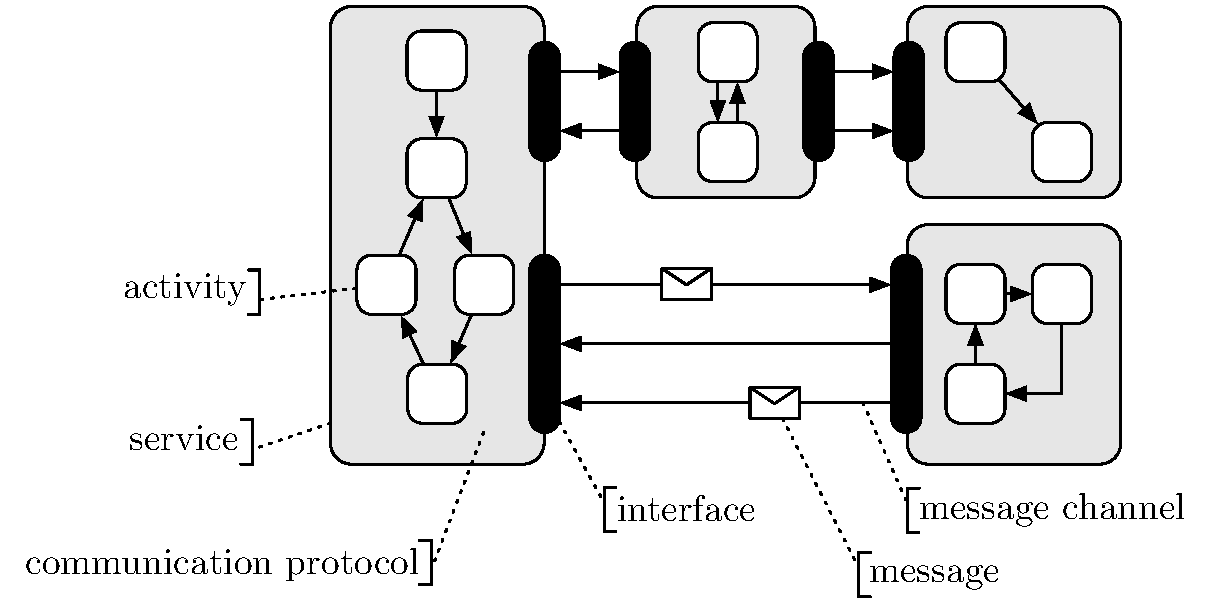
\includegraphics[scale=0.4]{introduction/overview}\hspace{4em}
\caption{A service composition.}
\label{fig:overview}
\end{figure}
%%%%%%%%%%%%%%%%%%%%%%%%%%%%%%%%%%%%%%%%%%%%%%%%%%%%%%%%%%%%%%%%%%%%%%%%%%%%%%

\noindent\emph{Service-oriented computing} (\acronym{SOC})~\cite{Papazoglou_2001_cacm} is an emerging paradigm of interorganizational cooperation. It aims at breaking complex monolithic systems into a composition of several simpler and self-contained, yet logically or geographically distributed components, called \emph{services}. A service has an identifier and offers an encapsulated functionality through a well-defined interface; see \autoref{fig:overview} for an illustration of the concepts. Services are open systems and are designed for being invoked by other services or for invoking other services themselves, and are typically not executed in isolation. Conceptually, \acronym{SOC} revives old ideas from component-based design~\cite{Mcilroy_1969_sect,Szyperski_1998_book} or from programming-in-the-large~\cite{DeRemerK_1976_tse}, for instance.

A simple realization of \acronym{SOC} is the encapsulation of classical computer programs which calculate an output from given inputs as \emph{remote procedure calls} or \emph{stateless services}. Such services only exchange pairs of request/response messages and are capable of implementing simple systems such as stock or weather information systems. This approach is insufficient to implement real-world business scenarios, which do not only calculate an output from given inputs, but in which messages are constantly sent back and forth. Examples for such \emph{stateful} conversations are price negotiations, auctioning, or scenarios in which exception handling is necessary. In this setting, more complex interactions need to be considered and a service needs to implement a \emph{communication protocol} (also called \emph{business protocol}~\cite{Papazoglou_2007_book}) which specifies the order in which the service's activities are executed and which may distinguish arbitrary states of the interaction with other services. The most prominent class of services are \emph{Web services}~\cite{AlonsoCKM_2003}. Here, the Internet and several Web-related standards are used to realize \acronym{SOC}. This makes services virtually independent of their geographical location and technological context and allows to entirely focus on the functions a service offers.

%%%%%%%%%%%%%%%%%%%%%%%%%%%%%%%%%%%%%%%%%%%%%%%%%%%%%%%%%%%%%%%%%%%%%%%%%%%%%%
\begin{figure}
\centering
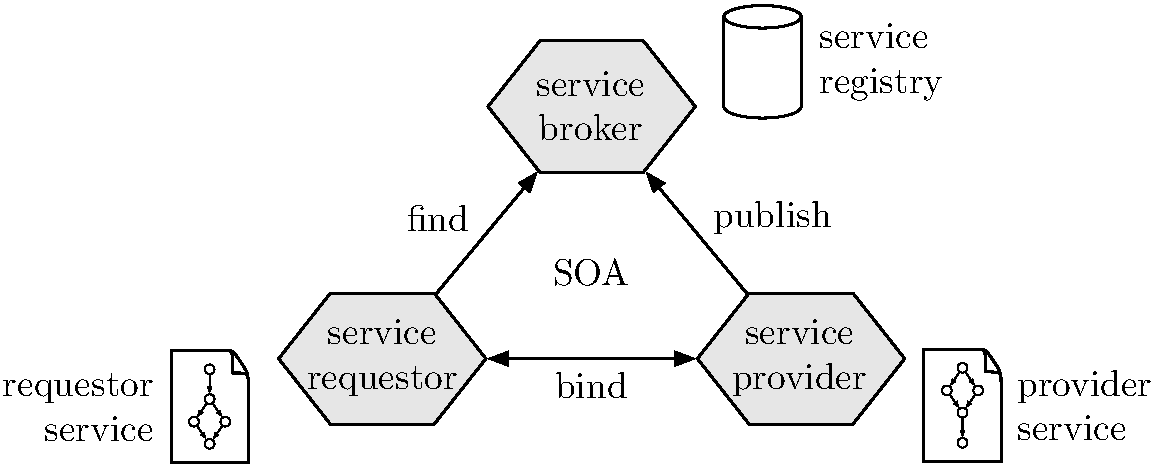
\includegraphics[scale=0.4]{introduction/soa-triangle}
\caption{The \acronym{SOA} triangle.}
\label{fig:soatriangle}
\end{figure}
%%%%%%%%%%%%%%%%%%%%%%%%%%%%%%%%%%%%%%%%%%%%%%%%%%%%%%%%%%%%%%%%%%%%%%%%%%%%%%

The idea of abstracting from underlying technologies and implementations makes it possible to compare services and to replace one service by another service which is, for instance faster, cheaper, compliant with new legal regulations, or more reliable. To this end, \acronym{SOC} allows to effortlessly replace, outsource, and optimize functionalities. This flexible binding is described as a \emph{service-oriented architecture} (\acronym{SOA})~\cite{Gottschalk00}. A \acronym{SOA} provides a general framework for service interaction. This framework\,---\,often called the \acronym{SOA} triangle\,---\,distinguishes three roles of services (as shown in \autoref{fig:soatriangle}). A \emph{service provider} publishes information about his service to a public registry. A \emph{service broker} manages the registry and allows a \emph{service requester} to find an adequate published service. Then, the provider and the requester may bind their services and start interaction.

%%%%%%%%%%%%%%%%%%%%%%%%%%%%%%%%%%%%%%%%%%%%%%%%%%%%%%%%%%%%%%%%%%%%%%%%%%%%%%
\begin{figure}
\centering
\hfill
\subfigure[service orchestration\label{fig:intro:orch}]{\includegraphics[scale=0.4]{introduction/orchestrator}}\hfill
\subfigure[service choreography\label{fig:intro:chor}]{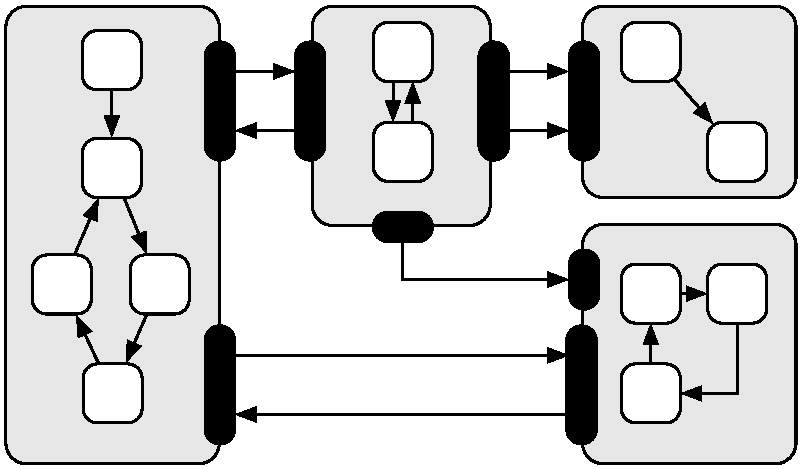
\includegraphics[scale=0.4]{introduction/choreography}} \hfill${}$
\caption{Service orchestration versus service choreography.}
\end{figure}
%%%%%%%%%%%%%%%%%%%%%%%%%%%%%%%%%%%%%%%%%%%%%%%%%%%%%%%%%%%%%%%%%%%%%%%%%%%%%%

In a \emph{service orchestration}, the flexibility to bind formerly unknown providers is employed to offer higher-value added services. It takes the viewpoint of a single participant in the service composition (the \emph{orchestrator}) and abstracts from the internal behavior of other participants. The orchestrator only considers the interfaces of the other participants rather than their concrete behavior or any interaction between third parties (see \autoref{fig:intro:orch}). Service orchestrations are well-suited to describe a business process whose activities are executed by other services.

Services can be also used to specify and implement an entire interorganizational business process. Such a business process is specified by several parties and explicitly or implicitly describes the behavior of each participant from a global perspective (see~\autoref{fig:intro:chor}). From this public description (also called \emph{contract} or \emph{service choreography}), each party derives its share and implements it as a service.

Services received much attention in industry and academia. This is reflected by many standardization efforts for several aspects of services. For instance, there exist various specification and programming languages for services orchestrations (\eg, \acronym{WS-BPEL}~\cite{standard_bpel} or \acronym{BPMN}~\cite{standard_bpmn}) and choreographies (\eg, \bpelchor~\cite{DeckerKLW_2007_icws}, \acronym{WS-CDL}~\cite{standard_wsdl}, i\acronym{BPMN}~\cite{DeckerB_2007_bpmw}, or \acronym{BPMN} 2.0 choreographies~\cite{standard_bpmn2}).





%%%%%%%%%%%%%%%%%%%%%%%%%%%%%%%%%%%%%%%%%%%%%%%%%%%%%%%%%%%%%%%%%%%%%%%%%%%%%%%
\section{Research goal}
%%%%%%%%%%%%%%%%%%%%%%%%%%%%%%%%%%%%%%%%%%%%%%%%%%%%%%%%%%%%%%%%%%%%%%%%%%%%%%%

Service-orientation allows to construct large distributed systems by composing several heterogenous and decentralized services. This modularization may reduce complexity and cost. At the same time, new challenges arise with the distributed execution of independent services in flexible compositions. In particular, the correctness of a service composition depends on the local correctness of each participating service \emph{and} the correct interaction between them. Unlike in a centralized monolithic system, parts of the system may change and are not completely controlled by a single party. Furthermore, a global state of the system and transitions between states are replaced by local states and local state transitions in addition to message transfer between parties.

Although services have been around for many years and several scientific communities focus on service-related topics, there do not exist widely accepted correctness criteria which are specific to services. From a practical point of view, a system composed of several services can be considered correct if it behaves just as well as a monolithic system. In particular, \emph{the participants should not be aware that the system consists of several decentrally executed components which implement a complex communication protocol and that have been bound without revealing specific implementation details}.

This brings us to the central research question which is investigated in this thesis:

%%%%%%%%%%%%%%%%%%%%%%%%%%%%%%%%%%%%%%%%%%%%%%%%%%%%%%%%%%%%%%%%%%%%%%%%%%%%%%
\begin{framed}
\noindent How can the design of correct services and service compositions be systematically supported?
\end{framed}
%%%%%%%%%%%%%%%%%%%%%%%%%%%%%%%%%%%%%%%%%%%%%%%%%%%%%%%%%%%%%%%%%%%%%%%%%%%%%%

This question touches upon several challenges:
\begin{niceitemize}
\item \emph{Formalization and verification of correctness.} How to formalize service behavior and correctness notions for services? Can correctness be automatically verified using model checking techniques?
\item \emph{Error detection and correction.} In case an error is detected, which participating services are responsible for this error? How can the overall system be fixed toward correct execution?
\item \emph{Compositional verification.} Can services be verified in isolation; that is, can local correctness of the participating services be used to derive global correctness of a service composition?
\item \emph{Correctness by construction.} Can the design of correct service compositions be supported in a systematic manner? Can errors be avoided in the first place rather than be detected a posteriori? Can service compositions be automatically derived from choreography specifications?
\item \emph{Applicability of correctness techniques.} Can the formal methods be applied to industrial services? Do the verification algorithms scale to models of industrial size?
\end{niceitemize}

As research goal of this thesis, we want to investigate these challenges on a behavioral level. That said, \emph{we only consider the communication protocol of services and service compositions and abstract from any other aspect which is not immediately related to behavior such as nonfunctional properties, semantics (\ie, ontologies), or instance life cycles}. Our approach complements those aspects: For instance, a proper treatment of semantic discrepancies between services is a prerequisite of our approach, but does not replace the necessity to send and receive messages in a suitable order. Policies and nonfunctional criteria can be integrated into our approach as far as they can be reduced to behavioral constraints. Nonfunctional properties are, however, not the focus of this thesis.





%%%%%%%%%%%%%%%%%%%%%%%%%%%%%%%%%%%%%%%%%%%%%%%%%%%%%%%%%%%%%%%%%%%%%%%%%%%%%%
\section{Contributions}
%%%%%%%%%%%%%%%%%%%%%%%%%%%%%%%%%%%%%%%%%%%%%%%%%%%%%%%%%%%%%%%%%%%%%%%%%%%%%%

The contributions of this thesis are all centered around correctness of services and their composition. Parts of the results of this thesis have been published in earlier papers~\cite{LohmannMW_2007_bpm,Lohmann_2008_wsfm,LohmannKLR_2007_wsfm,Lohmann_2008_bpm,LohmannW_2009_wsfm}. This thesis summarizes and extends these results. The work presented can be grouped into the following five categories.




%%%%%%%%%%%%%%%%%%%%%%%%%%%%%%%%%%%%%%%%%%%%%%%%%%%%%%%%%%%%%%%%%%%%%%%%%%%%%%
\subsection*{Contribution $\mathnormal{1}$: Formal foundation}

As motivated earlier, formal verification techniques require a formal model of the system under consideration. This thesis investigates correctness in a variety of settings of \acronym{SOC}. As a first contribution, we formalize the aspects sketched in \autoref{fig:overview} and define with \emph{service automata} a uniform formal model that is able to specify the behavior of single services, service compositions, and service choreographies. Using service automata, we define the correctness notions we shall investigate in the remainder of this thesis:

\begin{niceitemize}
\item \emph{Compatibility}. A service composition is \emph{compatible} iff (1) its execution only terminates in desired final states, (2) message channels are bounded, and (3)~nonterminating executions do not exclude a service. We are aware that there exist more sophisticated correctness criteria in literature, for instance, absence of livelocks as an additional requirement. However, our setting is certainly basic enough to be part of any other reasonable concept of correctness of service compositions. Therefore, it can be seen as an intermediate step toward more sophisticated settings.

\item \emph{Controllability}. A service is \emph{controllable}~\cite{Wolf_2008_topnoc} iff there exists another service such that their composition is compatible. Controllability is an extension of compatibility to single services and can be seen as a fundamental sanity property for services.

\item \emph{Realizability}. A choreography specification is \emph{realizable}~\cite{FuBS_2004_tcs,AlurEY_2003_tse} iff there exists a compatible service composition which exactly implements the specified interactions. Realizable choreography specifications follow a top-down modeling approach of service compositions which are compatible by design.
\end{niceitemize}

The employment of a single formalism throughout this thesis allows us to simplify theory, combine results, and to reuse algorithms and tools. In addition, the results of this thesis can be immediately applied to domain-specific service description languages as soon as a translation into service automata is available. In this thesis, we shall present such translations from \acronym{WS-BPEL} and \bpelchor{} into service automata.




%%%%%%%%%%%%%%%%%%%%%%%%%%%%%%%%%%%%%%%%%%%%%%%%%%%%%%%%%%%%%%%%%%%%%%%%%%%%%%
\subsection*{Contribution $\mathnormal{2}$: Correctness of services}

Compatibility can only be checked for complete service compositions. At design time of single services, such a complete composition is usually not available. To still make a statement on the correctness of a single service, its share of compatibility in \emph{any} possible composition can be analyzed using the notion of controllability. This thesis extends controllability in two aspects:

\begin{niceitemize}
\item \emph{Validation and selection}. In earlier work \cite{LohmannMW_2007_bpm}, we focused on the verification of services. We refined the notion of controllability with the help of behavioral constraints. These constraints can be seen as a specification of desired interactions a service can be checked against. If the specification is satisfied by the service, we can synthesize communication partners with the specified communication protocol. Furthermore, we show how a specification can be used to restrict a set of controllable services to only those which additionally satisfy a given specification.

\item \emph{Diagnosis}. Not every service is controllable. Unfortunately, the classical analysis algorithm to decide controllability~\cite{Wolf_2008_topnoc} lacks the possibility to provide counterexamples in case a service is uncontrollable. We studied this issue in \cite{Lohmann_2008_wsfm} and presented an algorithm to diagnose uncontrollable services. This diagnosis information (\ie, a counterexample for controllability) can help to understand the reasons which led to uncontrollability and proposes actions to fix them.
\end{niceitemize}




%%%%%%%%%%%%%%%%%%%%%%%%%%%%%%%%%%%%%%%%%%%%%%%%%%%%%%%%%%%%%%%%%%%%%%%%%%%%%%
\subsection*{Contribution $\mathnormal{3}$: Correctness of service compositions}

As described earlier, the composition of logically and geographically distributed services to a compatible overall system can be a challenging task. In this thesis, we propose the following techniques to ease the design of correct service compositions:

\begin{niceitemize}
\item \emph{Verification and completion}. Compatibility of \acronym{WS-BPEL} services and compositions of \acronym{WS-BPEL} services were analyzed in \cite{LohmannKLR_2007_wsfm}. We provide formal semantics for \bpelchor{} choreographies, which enables the application of existing formal methods to industrial service languages. This includes verification of compositions with respect to compatibility and the completion of partially specified service compositions.

\item \emph{Correction}. In case a service composition is not compatible, verification techniques usually provide a counterexample which describes a trace from the initial state to an error state. This trace usually spans over several services of the composition and gives little detail on how to fix the composition. To this end, we defined in \cite{Lohmann_2008_bpm} an algorithm to suggest changes of a service to achieve overall compatibility.
\end{niceitemize}




%%%%%%%%%%%%%%%%%%%%%%%%%%%%%%%%%%%%%%%%%%%%%%%%%%%%%%%%%%%%%%%%%%%%%%%%%%%%%%
\subsection*{Contribution $\mathnormal{4}$: Correctness of service choreographies}

A service composition can be built by composing several existing services. A different paradigm follows a top-down approach and globally specifies the interaction protocol, which should be implemented by the service composition. In case this choreography specification is realizable, it can be projected to several services whose composition is compatible and satisfies the specification by design. Our contribution to this topic is as follows.

\begin{niceitemize}
\item \emph{Realization}.
In \cite{LohmannW_2009_wsfm}, we studied the specification phase of service compositions. We refine existing realizability notions and link the problems related to choreographies to controllability. This allows us to apply all techniques we described so far to the area of choreographies.
\end{niceitemize}




%%%%%%%%%%%%%%%%%%%%%%%%%%%%%%%%%%%%%%%%%%%%%%%%%%%%%%%%%%%%%%%%%%%%%%%%%%%%%%
\subsection*{Contribution $\mathnormal{5}$: Tool support and experimental results}

All algorithms presented in this thesis are implemented in several open source free software tools which are available for download at \href{http://service-technology.org/tools}{http:/\!/service-technology.org/tools}. In particular, the following tools were developed in the course of this thesis.

\begin{niceitemize}
\item \emph{Wendy}~\cite{LohmannW_2009_wendy} synthesizes partners for services and implements the decision and diagnosis algorithm for controllability.
\item \emph{Rachel}~\cite{rachel} provides correction information and recommendations to fix an incompatible service composition toward compatibility.
\item \emph{Rebecca}~\cite{rebecca} analyzes choreography specifications for realizability and synthesizes realizing services.
\end{niceitemize}

We further used the tools \emph{LoLA}~\cite{Wolf_2007_icatpn} and \emph{Fiona}~\cite{MassutheW_2008_awpn} to support additional scenarios investigated in this thesis. In addition, we use the compiler \emph{BPEL$\mathit{2}$oWFN}~\cite{Lohmann_2007_hubtr212} to translate industrial services into formal models. Although all tools are proof of concept implementations, experimental results demonstrate the principal feasibility of the approaches. Where possible, we used realistic models translated from \acronym{WS-BPEL} services provided by industrial project partners.





%%%%%%%%%%%%%%%%%%%%%%%%%%%%%%%%%%%%%%%%%%%%%%%%%%%%%%%%%%%%%%%%%%%%%%%%%%%%%%%
\section{Outline}
%%%%%%%%%%%%%%%%%%%%%%%%%%%%%%%%%%%%%%%%%%%%%%%%%%%%%%%%%%%%%%%%%%%%%%%%%%%%%%%

The aforementioned list of results sketches an outline for the remainder of this thesis which is illustrated in \autoref{fig:parts}.

\medskip

%%%%%%%%%%%%%%%%%%%%%%%%%%%%%%%%%%%%%%%%%%%%%%%%%%%%%%%%%%%%%%%%%%%%%%%%%%%%%%
\begin{figure}
\centering
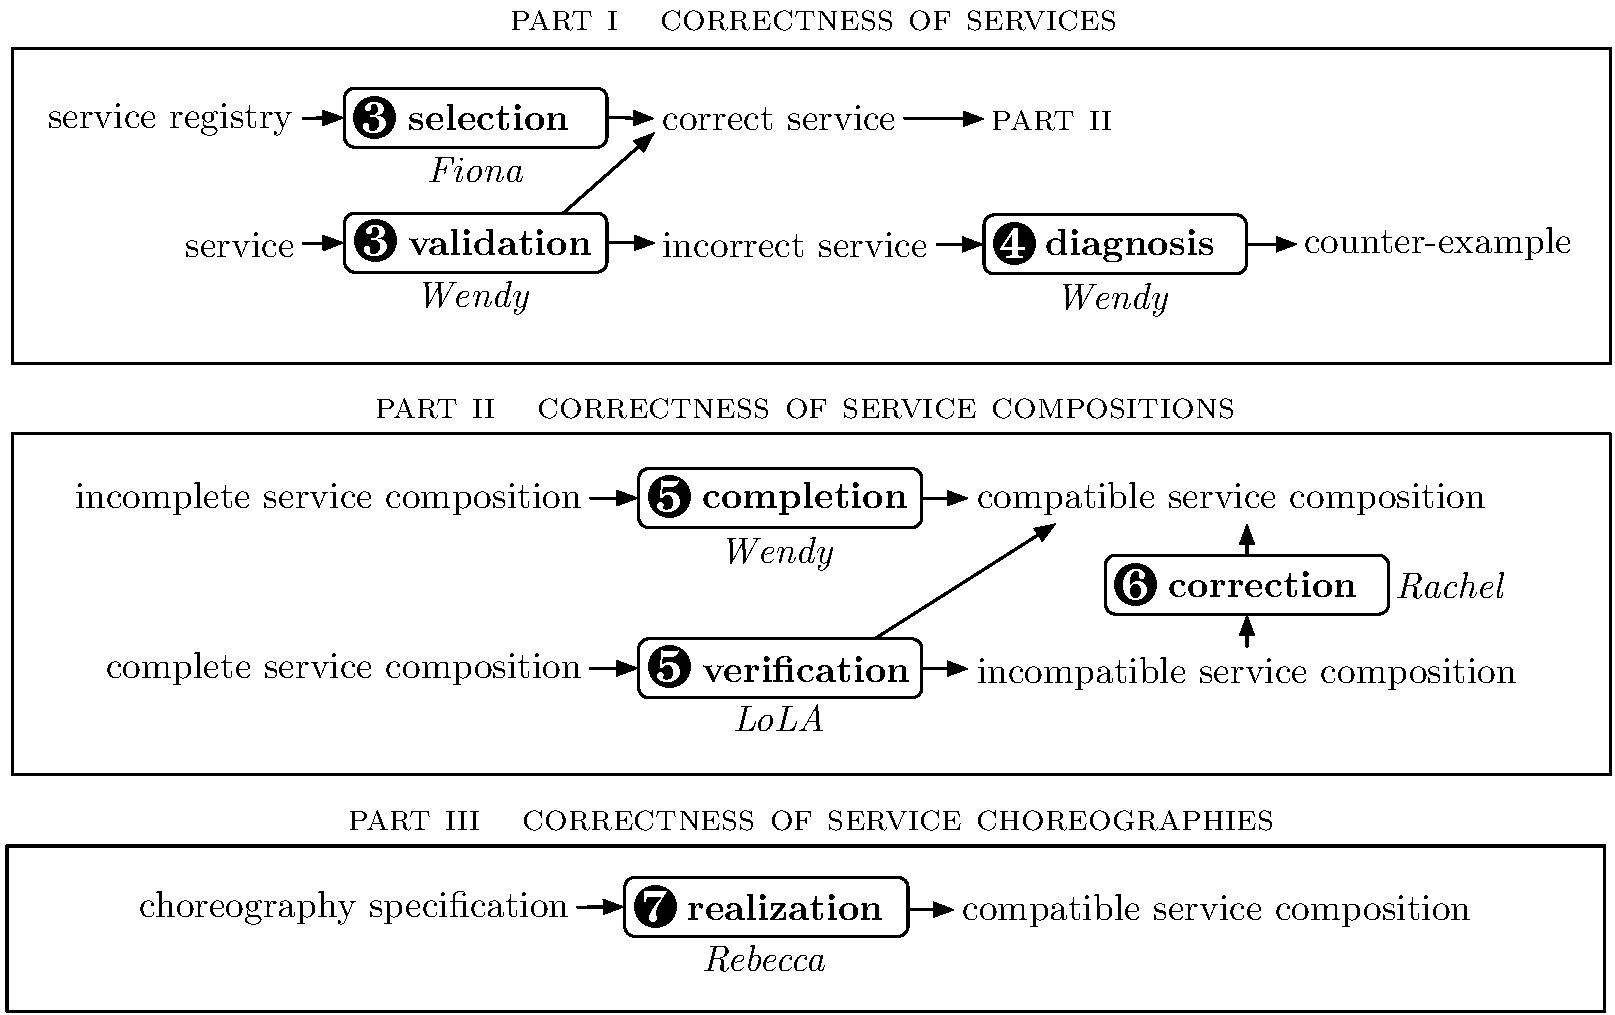
\includegraphics[scale=0.4]{introduction/parts}
\caption{Interrelation of the \textbf{results}, \ding{183} chapters, and \emph{tools}.}\label{fig:parts}
\end{figure}
%%%%%%%%%%%%%%%%%%%%%%%%%%%%%%%%%%%%%%%%%%%%%%%%%%%%%%%%%%%%%%%%%%%%%%%%%%%%%%

The next chapter provides the basic definitions and notions we employ throughout the thesis. It introduces the formal framework we use to model services and service compositions. Furthermore, the correctness criteria introduced informally in this chapter are defined in terms of the formal model. Finally, existing concepts to represent the set of partners of a service are briefly recapitulated.

\medskip

The remainder of the thesis is divided into three parts, each studying a service-oriented system from a different point of view. We present the software tools used and experimental results obtained within the context of the respective chapters.

\begin{niceitemize}
\item \spacedlowsmallcaps{Part I}.\quad The first part is dedicated to correctness criteria which can be expressed and checked with respect to a single service. The refinement of the controllability notion to validate  services is described in \autoref{chap:validation}, together with various application scenarios of this notion, for instance the selection of services from a service registry. \Autoref{chap:diagnosis} focuses on diagnostic information (viz.\ the construction of counterexamples) in case a service is uncontrollable.

\item \spacedlowsmallcaps{Part II}.\quad In the second part, we go one step further and consider the correctness of service compositions. In \autoref{chap:verification}, we show how compatibility of industrial service compositions defined in \bpelchor{} can be verified and how a completion algorithm can support the construction of compatible compositions. \Autoref{chap:correction} shows how correction proposals for incorrect service compositions can be automatically derived.

\item \spacedlowsmallcaps{Part III}.\quad In the last part of the thesis, we study a correctness-by-construction approach for service compositions. Given a choreography specification, we investigate whether this global specification can be realized by several services. \Autoref{chap:realizability} shows how the realizability problem of services can be approached in terms of controllability. This link makes all results of the previous chapters applicable to service choreographies.
\end{niceitemize}

\medskip

\Autoref{chap:conclusion} concludes the thesis and summarizes the contributions and the remaining open problems. Furthermore, it sketches directions for future extensions of the presented results.

\chapter{Formal models for services}
\label{chap:formal}

\lettrine[findent=.2em,lines=2,nindent=0pt]{I}{n} this chapter, we introduce the basic concepts used in the remainder of this thesis. In particular, we introduce \emph{service automata} as a uniform formalism to define the behavior of a service and a service composition. Based on service automata, we define the correctness notions we investigate in the subsequent chapters. We continue by recalling algorithms to construct and characterize correct service automata. We conclude the chapter with a discussion on the choice of service automata as our formal model.





%%%%%%%%%%%%%%%%%%%%%%%%%%%%%%%%%%%%%%%%%%%%%%%%%%%%%%%%%%%%%%%%%%%%%%%%%%%%%%%
\section{Preliminaries}
%%%%%%%%%%%%%%%%%%%%%%%%%%%%%%%%%%%%%%%%%%%%%%%%%%%%%%%%%%%%%%%%%%%%%%%%%%%%%%%

We first recall basic mathematical notions and define several fundamental concepts from computer science.


\paragraph{Sets}
\nomenclature[2M]{$2^M$}{the powerset of $M$}%
\nomenclature[N1]{$\mathds{N}$}{the set of natural numbers (including $0$)}%
\nomenclature[N1+]{$\mathds{N}^+$}{the set of positive natural numbers (excluding $0$)}%

For a set $M$, we denote its cardinality with $|M|$ and its powerset with \smash{$2^M$}. We denote the set of natural numbers (including~$0$) with $\mathds{N}$ and the set of positive natural numbers (excluding~$0$) with~$\mathds{N}^{+}$.


\paragraph{Multisets}
\nomenclature[B]{$\mathcal{B}$}{a multiset}%
\nomenclature[BagsM]{$\Bags(M)$}{the set of all multisets over the set $M$}%
\nomenclature[BagsM]{$\Bags_{k}(M)$}{the set of all $k$-bounded multisets over the set $M$}%
\nomenclature{$\emptymset$}{the empty multiset}%

We denote the set of all multisets over a set $M$ with $\Bags(M)$. We use the list notation for multisets and, for example, write $[x,y,y]$ for the multiset $\{x\mapsto 1, y\mapsto 2, z\mapsto 0\}$ over $\{x,y,z\}$; $\emptymset$ denotes the empty multiset. Addition of multisets $\mathcal{B}_{1},\mathcal{B}_{2}\in\Bags(M)$ is defined pointwise: $(\mathcal{B}_{1}+\mathcal{B}_{2})(x):=\mathcal{B}_{1}(x)+\mathcal{B}_{2}(x)$, for all $x\in M$. For $k\in\mathds{N}$, we denote with $\Bags_{k}(M)$ the set of multisets such that $\mathcal{B}\in\Bags_{k}(M)$ implies $\mathcal{B}(x)\leq k$, for all $x\in M$.


\paragraph{Labeled transition systems}
\nomenclature[q]{$q$}{a state ($q\in Q$)}%
\nomenclature[Q]{$Q$}{a set of states}%
\nomenclature[q0]{$q_{0}$}{the initial state ($q_{0}\in Q$)}%
\nomenclature{$\shortrightarrow$}{a transition relation}%

In this thesis, we distinguish visible (\ie, communicating) and invisible (\ie, internal) actions, yielding an extended definition of labeled transition systems: A \define{labeled transition system} $T=[Q,q_{0},\Sigma,\Sigma^{\tau},{\shortrightarrow}]$ consists of a set of states~$Q$, an initial state~$q_{0}\in Q$, a~set of visible labels~$\Sigma$, a set of \emph{discriminable invisible} labels~$\Sigma^{\tau}$ with $\Sigma\cap\Sigma^{\tau}=\emptyset$, and a~labeled transition relation~${\shortrightarrow}\subseteq Q\times(\Sigma\cup\Sigma^{\tau})\times Q$. For $[q,x,q']\in{\shortrightarrow}$, we shall write~\smash{$q\xrightarrow{x}q'$}. If not clear from the context, we add indices to the constituents of $T$ and refer to its states by $Q_{T}$, for instance.

A state $q'\in Q$ is \define{reachable from a state $q\in Q$}, denoted \smash{$q\xrightarrow{*}q'$}, iff there exists a (possibly empty) sequence of transitions originating in $q$ and ending in $q'$. A state is \define{reachable} iff it is reachable from the initial state~$q_{0}$. If $q$ has no outgoing transitions, we also write $q\not\xrightarrow{}{}$. We define the set $\tau(q)$ of \define{internally reachable states} for a state $q\in Q$ inductively as follows: (base) $q\in \tau(q)$ and (step) if $q'\in \tau(q)$ and \smash{$q'\xrightarrow{x}q''$} with $x\in\Sigma^{\tau}$, then $q''\in \tau(q)$.

For a state $q\in Q$, we define \smash{$\lab(q):=\{x\in\Sigma\mid \exists q'\in Q: q\xrightarrow{x}q'\}$} and $\lab^*(q):=$\break \smash{$\bigcup_{q'\in \tau(q)} \lab(q')$}. A transition system $T$ is \define{complete} iff $\lab(q)=\Sigma$ for each reachable state $q\in Q$. $T$ is \define{deterministic} iff  \smash{$q\xrightarrow{x}q'$} and \smash{$q\xrightarrow{x}q''$} implies $q'=q''$ for each reachable state $q\in Q$. $T$ is \define{$\tau$-free}, if \smash{$q\xrightarrow{x}q'$} implies $x\in\Sigma$ for each reachable state $q\in Q$. $T$ is a \define{finite state} transition system, iff the number of reachable states is finite.

A \define{strongly connected component} (\acronym{SCC}) of $T$ is a maximal set of states $Q'\subseteq Q$ such that $q,q'\in Q'$ implies \smash{$q\xrightarrow{*}q'$}. An \acronym{SCC} $Q'$ is a \define{terminal strongly connected component} iff, for all $q\in Q'$, $q\xrightarrow{*}q'$ implies $q'\in Q'$.


\paragraph{Simulation and structural matching}\label{def:smatching}
\nomenclature[rho]{$\rho$}{a simulation or structural matching relation}%

Let $T$ and $U$ be labeled transition systems. A relation $\varrho\subseteq Q_{T}\times Q_{U}$ is a \define{simulation relation}, iff $[q_{0_{T}},q_{0_{U}}]\in\varrho$ and for all states $q_{T},q'_{T}\in Q_{T}$, all states $q_{U}\in Q_{U}$, and for all labels $x\in\Sigma\cup\Sigma^\tau$ holds: if $[q_{T},q_{U}]\in\varrho$ and \smash{$q_{T}\xrightarrow{x}_{T}q_{T}'$}, then there exists a state $q_{U}'\in Q_{U}$ such that \smash{$q_{U}\xrightarrow{x}_{U}q_{U}'$} and $[q_{T}',q_{U}']\in\varrho$.

We use the distinction between visible and invisible labels to define another relation between states of two transition systems: A relation $\varrho\subseteq Q_{T}\times Q_{U}$ is a \define{structural matching relation}, iff $[q_{0_{T}},q_{0_{U}}]\in\varrho$ and for all states $q_{T},q_{T}'\in Q_{T}$, all states $q_{U}\in Q_{U}$, and for all labels $x\in\Sigma\cup\Sigma^\tau$ holds: if $[q_{T},q_{U}]\in\varrho$ and \smash{$q_{T}\xrightarrow{x}_{T}q_{T}'$}, then (1)~there exists a state $q_{U}'\in Q_{U}$ with \smash{$q_{U}\xrightarrow{x}_{U}q_{U}'$} and $[q_{T}',q_{U}']\in\varrho$ or (2) $x\in\Sigma^{\tau}$ and $[q_{T}',q_{U}]\in\varrho$. The first requirement is the same as for a simulation relation. The second requirement allows the transition system~$T$ to take an arbitrary number of invisible transitions. This makes a structural matching relation similar to a weak simulation relation or a stuttering simulation relation~\cite{BrowneCG_1988_tcs}, but stuttering is only allowed in the labeled transition system $T$.

%%%%%%%%%%%%%%%%%%%%%%%%%%%%%%%%%%%%%%%%%%%%%%%%%%%%%%%%%%%%%%%%%%%%%%%%%%%%%%
\begin{figure}[tb]
\centering
\subfigure[simulation relation]{\makebox[0.49\textwidth]{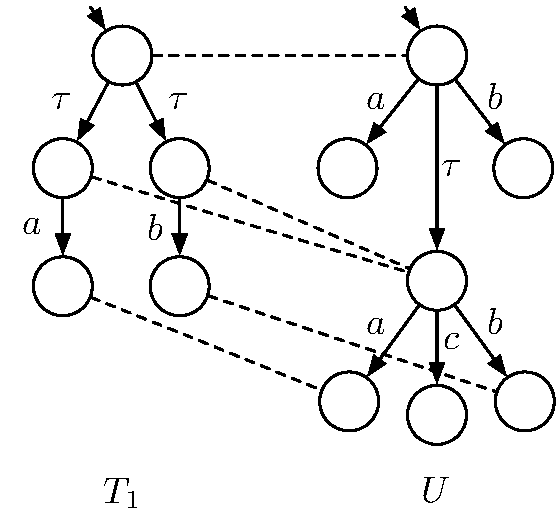
\includegraphics[scale=0.4]{background/simulation}}}\hfill
\subfigure[structural matching relation]{\makebox[0.49\textwidth]{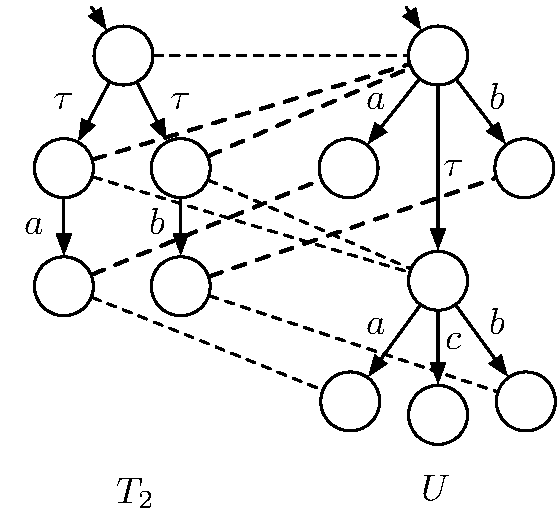
\includegraphics[scale=0.4]{background/matching}}}
\caption{Simulation and structural matching.}
\label{fig:simulationmatching}
\end{figure}
%%%%%%%%%%%%%%%%%%%%%%%%%%%%%%%%%%%%%%%%%%%%%%%%%%%%%%%%%%%%%%%%%%%%%%%%%%%%%%%

A transition system $U$ \define{simulates} (\define{structurally matches}) a transition system $T$ iff there exists a simulation relation (a structural matching relation) $\varrho\subseteq Q_{T}\times Q_{U}$. If the transition systems $T$ and $U$ are not clear from the context, we shall add indices and write $\varrho_{(T,U)}$. \Autoref{fig:simulationmatching} illustrates the simulation and structural matching relation.






%%%%%%%%%%%%%%%%%%%%%%%%%%%%%%%%%%%%%%%%%%%%%%%%%%%%%%%%%%%%%%%%%%%%%%%%%%%%%%%
\section{Modeling services and their composition}
%%%%%%%%%%%%%%%%%%%%%%%%%%%%%%%%%%%%%%%%%%%%%%%%%%%%%%%%%%%%%%%%%%%%%%%%%%%%%%%

%\enlargethispage*{\baselineskip}

In this section, we elaborate the core definitions for services and service compositions. We shall introduce the concept of \emph{ports} to model the (purely syntactic) \emph{interface} of a service. To specify the actual behavior of a service (\ie,~the order in which messages are sent or received), we employ \emph{service automata}.

\medskip

\nomenclature[M-]{$\M$}{the set of all message channels}%
\nomenclature[M-as]{$\M_{s}$}{the set of all synchronous message channels}%
\nomenclature[M-a]{$\M_{a}$}{the set of all asynchronous message channels}%
\nomenclature[E?]{$\E$}{the set of all message events}%
\nomenclature[E?a]{$\send\E$}{the set of all asynchronous send message events}%
\nomenclature[E?b]{$?\E$}{the set of all asynchronous receive message events}%
\nomenclature[E?c]{$\sync\E$}{the set of all synchronous message events}%
\nomenclature[tau]{$\tau$}{a noncommunicating event ($\tau\notin\E$)}%
\nomenclature[M-e]{$\M(e)$}{the message channel of an event $e\in \E$}%
Throughout this thesis, we fix a finite set of message channels $\M$ that is partitioned into asynchronous message channels $\M_{a}$ and synchronous message channels $\M_{s}$. From $\M$, we derive a set of message events $\E$ that is partitioned into asynchronous send events ${!\E}:=\{!m\mid m\in \M_{a}\}$, asynchronous receive events ${?\E}:=\{?m\mid m\in \M_{a}\}$, and synchronous events ${\sync\E}:=\{\sync m\mid m\in \M_{s}\}$. Furthermore, we distinguish a noncommunicating event $\tau\notin \E$. For an event $e\in\{!m, ?m, \sync m\}$, define its message channel as $\M(e):=m$.

In the following definition, we give message channels a direction and group them into \emph{ports} from which we build \emph{interfaces}. An interface lists the ``open'' message channels that are exposed to the environment; that is, to other services. Interfaces can be composed by connecting open message channels. This yields ``closed'' message channels that cannot be used by other services. In this thesis, such closed message channels still belong to the interface. They can be seen as the ``composition history'' of the respective service automaton that implements the interface. This simplifies subsequent definitions and allows for a unified formal model throughout this thesis.

%%%%%%%%%%%%%%%%%%%%%%%%%%%%%%%%%%%%%%%%%%%%%%%%%%%%%%%%%%%%%%%%%%%%%%%%%%%%%%%
\begin{definition}{Port, interface, closed interface}%
\label{def:interface}%
\nomenclature[I]{$I$}{the input message channel of a port $P=[I,O]$}%
\nomenclature[O]{$O$}{the output message channel of a port $P=[I,O]$}%
\nomenclature[Ep]{$\E_{P}$}{the events of a port $P$}%
\nomenclature[M-P]{$\M^{\closed}_{\mathcal{P}}$}{the closed message channels of an interface $\mathcal{P}$}%
\nomenclature[M-P]{$\M^{\open}_{\mathcal{P}}$}{the open message channels of an interface $\mathcal{P}$}%
\nomenclature[EPtau]{$\E^{\tau}_{\mathcal{P}}$}{the internal events of an interface $\mathcal{P}$}%
\nomenclature[EPex]{$\E_{\mathcal{P}}$}{the external events of an interface $\mathcal{P}$}%
%
A pair $P=[I,O]$ is a \define{port} iff $I\cup O\subseteq\M$ and $I\cap O=\emptyset$. $I$ and $O$ are the \define{input message channels} and \define{output message channels} of port $P$, respectively. For $P$, define its events as $\E_{P}:=\{{?m}\mid m\in I\cap \M_{a}\}\cup \{{!m}\mid m\in O\cap \M_{a}\} \cup \,\{{\sync m}\mid m\in (I\cup O)\cap \M_{s}\}$.

Let, for $n\in\mathds{N}$, $\mathcal{P}=\{P_{1},\ldots,P_{n}\}$ be a set of ports with $P_{i}=[I_{i},O_{i}]$ for $i\in\{1,\ldots,n\}$. $\mathcal{P}$ is an \define{interface} iff $I_{i}\cap I_{j}=\emptyset$ for all $i\neq j$ and $O_{i}\cap O_{j}=\emptyset$ for all $i\neq j$. Interface $\mathcal{P}$ is  \define{closed} iff $\bigcup_{i=1}^n I_{i}=\bigcup_{i=1}^n O_{i}$.

From $\mathcal{P}$, derive the set of \define{closed message channels} $\M^{\closed}_{\mathcal{P}}:=(\bigcup_{i=1}^n I_{i})\cap(\bigcup_{i=1}^n O_{i})$, the set of \define{open message channels} $\M^{\open}_{\mathcal{P}}:=(\bigcup_{i=1}^n(I_{i}\cup O_{i}))\setminus\M^{\closed}_{\mathcal{P}}$, the set of \define{internal events} $\E^{\tau}_{\mathcal{P}}:=\{e\in\bigcup_{i=1}^n\E_{P_{i}}\mid \M(e)\in\M^{\closed}_{\mathcal{P}}\}\cup\{\tau\}$, and the set of \define{external events} $\E_{\mathcal{P}}:=\{e\in\bigcup_{i=1}^n\E_{P_{i}}\mid \M(e)\in\M^{\open}_{\mathcal{P}}\}$.
\end{definition}
%%%%%%%%%%%%%%%%%%%%%%%%%%%%%%%%%%%%%%%%%%%%%%%%%%%%%%%%%%%%%%%%%%%%%%%%%%%%%%%

In a port, each message channel has a direction and is either an input message channel or an output message channel. This is natural for asynchronous communication where sending and receiving of messages is decoupled. In contrast, synchronous communication is usually undirected. The classification into input and output is of technical nature and can be compared to the complementary labels $a$ and $\overline{a}$ in \acronym{CCS}~\cite{Milner_1980_ccs}. Nevertheless, the semantics of a message on a finer level of abstraction may induce a natural initiator. For instance, an asynchronous handshake between two parties (\eg,~a pair of a request and an acknowledge message) can be abstracted to an atomic synchronization event.

An interface consists of a set of ports such that communication is bilateral. \emph{A message channel can be used by at most one port as input message channel and by at most one port as output message channel.} If a message channel is used by two ports that way, it is closed and not accessible by other ports any more. This corresponds to \emph{hiding} in process algebra~\cite{Baeten_2005_tcs}. From the message channels of a port and their direction, potential events can be derived. These events can be partitioned into internal events (including~$\tau$) and external events depending on whether the respective message channel is open or closed.

Depending on the context, an interface can be interpreted differently: for a single service, open message channels are exposed to the environment which can invoke the service. An interface with more than one port can be used to model a service orchestrator that interacts with several services simultaneously. In \acronym{WS-BPEL}~\cite{standard_bpel}, the term \emph{partner link} has been coined for such a partition of an interface. Finally, a closed interface describes a choreography of services (cf.~\autoref{chap:realizability}). In this scenario, no message channel is exposed to the environment: the sender and receiver of each message is specified. This \emph{closed world assumption} is common in choreography description languages such as \bpelchor~\cite{DeckerKLW_2007_icws} or \acronym{WS-CDL}~\cite{standard_wscdl}.

Ports and interfaces only describe the syntactic signature of a service consisting of an alphabet of possible events. The behavior itself (\ie,~the order in which messages exchange occurs and when a service terminates) is modeled by \emph{service automata}. A service automaton is a state machine whose transitions are labeled with events derived from a given interface.

%%%%%%%%%%%%%%%%%%%%%%%%%%%%%%%%%%%%%%%%%%%%%%%%%%%%%%%%%%%%%%%%%%%%%%%%%%%%%%%
\begin{definition}{Service automaton}%
\label{def:sa}%
\nomenclature[A]{$A$}{a service automaton}%
\nomenclature[W]{$\Omega$}{a set of final states ($\Omega\subseteq Q$)}%
\nomenclature[P]{$\mathcal{P}$}{an interface}%
A tuple $A=[Q,q_{0},{\shortrightarrow},\Omega,\mathcal{P}]$ is a \define{service automaton} iff
\begin{myitemize}
\item $\mathcal{P}$ is an interface,
\item $[Q,q_{0},\E_{\mathcal{P}},\E_{\mathcal{P}}^{\tau},{\shortrightarrow}]$ is a labeled transition system, and
\item $\Omega\subseteq Q$ is a set of final states.
\end{myitemize}
$A$ is a \define{single-port service automaton}, iff $|\mathcal{P}|=1$; otherwise, $A$ is a \define{multi-port service automaton}. $A$ is \define{closed}, iff $\mathcal{P}$ is a closed interface; otherwise, $A$ is \define{open}.
\end{definition}
%%%%%%%%%%%%%%%%%%%%%%%%%%%%%%%%%%%%%%%%%%%%%%%%%%%%%%%%%%%%%%%%%%%%%%%%%%%%%%%

A service automaton \emph{implements} the ports of its interface by labeling its state transitions with events. If a service automaton implements more than one port, message channels can be closed and the respective events are internal. Whereas internal events can occur independently of the service's environment, external message events can only be realized together with other services. This interplay with other services is defined in terms of the \emph{composition} of service automata.

%%%%%%%%%%%%%%%%%%%%%%%%%%%%%%%%%%%%%%%%%%%%%%%%%%%%%%%%%%%%%%%%%%%%%%%%%%%%%%%
\begin{definition}{Composition of service automata}
\label{def:composition}%
\nomenclature{$\oplus$}{composition of service automata}%
Two service automata $A$ and $B$ are \define{composable} iff $\mathcal{P}_{A}\cap\mathcal{P}_{B}=\emptyset$ and $\mathcal{P}_{A}\cup\mathcal{P}_{B}$ is an interface.

The \define{composition} of two composable service automata $A$ and $B$ is the service automaton $A\oplus B=[Q,q_{0},{\shortrightarrow},\Omega,\mathcal{P}]$ consisting of
\begin{myitemize}
\item $Q:=Q_{A}\times Q_{B}\times \Bags(\M_{a})$,
\item $q_{0}:=[q_{0_{A}},q_{0_{B}}, \emptymset]$,
\item $\Omega:={\Omega_{A}\times \Omega_{B}\times \{\emptymset\}}$,
\item $\mathcal{P}:=\mathcal{P}_{A}\cup\mathcal{P}_{B}$, and
\item ${\shortrightarrow}$ containing exactly the following elements:
\begin{enumerate}
\item for all $m\in\M_{\mathcal{P}_{A}}^{\open} \cap \M_{\mathcal{P}_{B}}^{\open}$ (shared open message channels) and $\mathcal{B}\in\Bags(\M_{a})$,
\begin{myitemize}
\item $[q_{A},q_{B},\mathcal{B}] \xrightarrow{!m} [q_{A}',q_{B},\mathcal{B}+[m]]$, iff $q_{A}\xrightarrow{!m}_{A} q_{A}'$,
\item $[q_{A},q_{B},\mathcal{B}] \xrightarrow{!m} [q_{A},q_{B}',\mathcal{B}+[m]]$, iff $q_{B}\xrightarrow{!m}_{B} q_{B}'$,
\item $[q_{A},q_{B},\mathcal{B}+[m]] \xrightarrow{?m} [q_{A}',q_{B},\mathcal{B}]$, iff $q_{A}\xrightarrow{?m}_{A} q_{A}'$,
\item $[q_{A},q_{B},\mathcal{B}+[m]] \xrightarrow{?m} [q_{A},q_{B}',\mathcal{B}]$, iff  $q_{B}\xrightarrow{?m}_{B} q_{B}'$,
\item $[q_{A},q_{B},\mathcal{B}] \xrightarrow{\sync m} [q_{A}',q_{B}',\mathcal{B}]$, iff $q_{A}\xrightarrow{\sync m}_{A} q_{A}'$ and $q_{B}\xrightarrow{\sync m}_{B} q_{B}'$;
\end{myitemize}
\item for $e\in\E_{\mathcal{P}_{A}}^{\tau}\cup\E_{\mathcal{P}_{B}}^{\tau}$ (internal events) or $e\in\E_{\mathcal{P}}$ (external events) and $\mathcal{B}\in\Bags(\M_{a})$,
\begin{myitemize}
\item $[q_{A},q_{B},\mathcal{B}] \xrightarrow{e} [q_{A}',q_{B},\mathcal{B}]$, iff $q_{A}\xrightarrow{e}_{A} q_{A}'$,
\item $[q_{A},q_{B},\mathcal{B}] \xrightarrow{e} [q_{A},q_{B}',\mathcal{B}]$, iff $q_{B}\xrightarrow{e}_{B} q_{B}'$.
\end{myitemize}
\end{enumerate}
\end{myitemize}
\end{definition}
%%%%%%%%%%%%%%%%%%%%%%%%%%%%%%%%%%%%%%%%%%%%%%%%%%%%%%%%%%%%%%%%%%%%%%%%%%%%%%%

The composability criteria require that the two services must not share a port (\ie,~each port is implemented by exactly one service automaton) and that their union still has the interface property of unidirectional and bilateral communication. Here, keeping closed message channels in the interface is important to keep track of the ``composition history'' of a service.

The composition of two service automata implements the union of their ports. For the state transitions, we distinguish two cases: (1)~communication events between the composed services and (2)~other events that are either internal to one of the composed services or external to the composition. Shared message events do not only influence a service's state, but may also add messages to or remove messages from an asynchronous message channel. To this end, each state of the composition contains a multiset of asynchronously sent messages that have not yet been received and that are pending on the message channel. This represents lossless asynchronous message passing under the assumption that messages can overtake each other. Synchronization between two services does not influence the pending messages. The message buffer is defined to be empty in the initial state and is required to be empty in the final states. The latter requirement rules out interactions that terminate without considering pending messages.

As notational convention, we identify the states of a composition of more than two services by a combination of the participating services' states and a sum of the pending asynchronous messages. For example, we do not identify a state of the composition $(A\oplus B)\oplus C$ with $[ [q_{A},q_{B},\mathcal{B}_{(A\oplus B)}], q_{C}, \mathcal{B}_{(A\oplus B)\oplus C} ]$, but with $[q,\mathcal{B}]$ for $q:=[q_{A},q_{B},q_{C}]$ and $\mathcal{B}:=\mathcal{B}_{A\oplus B}+\mathcal{B}_{(A\oplus B)\oplus C}$. Due to the requirement of bilateral communication and the retainment of closed ports, the composition is\,---\,up to isomorphism\,---\,commutative and associative. Hence, we may treat composition as a partial operation and write $A\oplus B\oplus C$ instead of $(A\oplus B)\oplus C$.


\paragraph{Example.}

As running example for this chapter, consider the service automaton depicted in \autoref{fig:Abuy}. It models a buyer service that receives offers ($o$) from a client and decides whether to accept~($a$) or to reject ($r$) the offer. This decision is modeled by internal $\tau$-steps and is nondeterministic. In case the offer got rejected, the service returns to its initial state ($q_{0}$) and waits for another offer. In case the offer got accepted, the service eventually receives an invoice ($i$) and reaches the final state ($q_{5}$). As it can be seen from the graphical representation, the message channels $a$, $r$, and $i$ are asynchronous, whereas $o$ is a synchronous channel.

\Autoref{fig:Asell} depicts a composable service automaton modeling a seller service. It sends offers until one gets accepted. The composition of the buyer and the seller service yields the closed service automaton in \autoref{fig:composition}. Throughout this thesis, we shall never depict unreachable states.


%%%%%%%%%%%%%%%%%%%%%%%%%%%%%%%%%%%%%%%%%%%%%%%%%%%%%%%%%%%%%%%%%%%%%%%%%%%%%%
\begin{figure}
\centering
\hfill
\subfigure[$A_\text{Buy}$\label{fig:Abuy}]{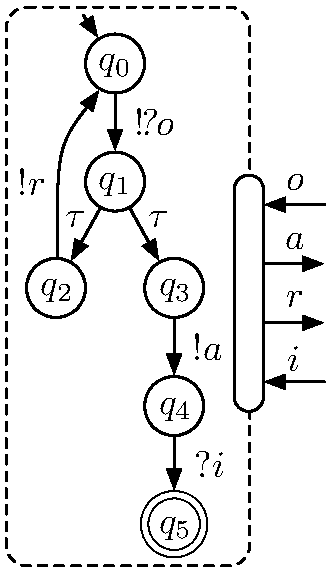
\includegraphics[scale=0.45]{background/running_sa}}\hfill
\subfigure[$A_\text{Sell}$\label{fig:Asell}]{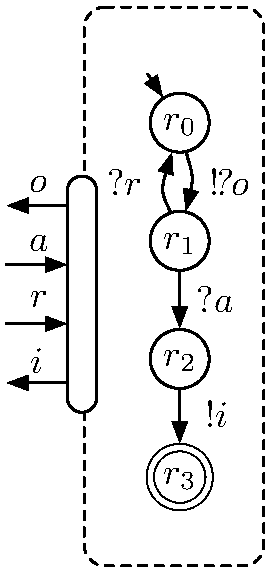
\includegraphics[scale=0.45]{background/running_client}}\hfill
\subfigure[$A_\text{Buy}\oplus A_\text{Sell}$\label{fig:composition}]{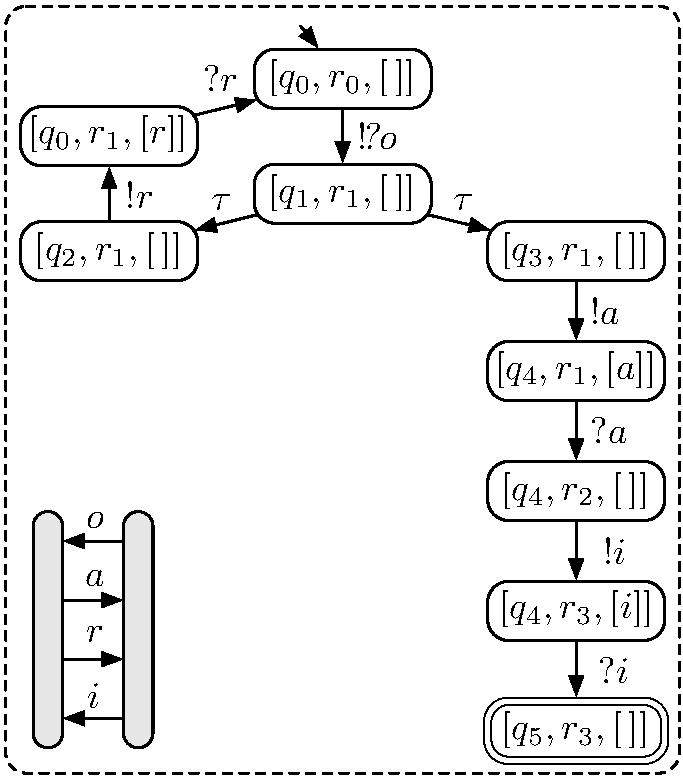
\includegraphics[scale=0.45]{background/running_composition}}\hfill{}
\caption{A buyer service $A_\text{Buy}$ (a) and a seller service $A_\text{Sell}$ (b) modeled as service automata. These automata are composable and (c) depicts their composition $A_\text{Buy}\oplus A_\text{Sell}$.}
\end{figure}
%%%%%%%%%%%%%%%%%%%%%%%%%%%%%%%%%%%%%%%%%%%%%%%%%%%%%%%%%%%%%%%%%%%%%%%%%%%%%%





%%%%%%%%%%%%%%%%%%%%%%%%%%%%%%%%%%%%%%%%%%%%%%%%%%%%%%%%%%%%%%%%%%%%%%%%%%%%%%%
\section{Correctness notions for services}
\label{sect:correctness}
%%%%%%%%%%%%%%%%%%%%%%%%%%%%%%%%%%%%%%%%%%%%%%%%%%%%%%%%%%%%%%%%%%%%%%%%%%%%%%%

Services are not executed in isolation, but are designed to communicate with other services. To this end, reasoning about a service's behavior only makes sense if it is part of a closed composition; that is, all message channels are closed and all events are internal. The behavior of a closed composition can then be defined with the concept of \emph{runs}.

\enlargethispage*{\baselineskip}

%%%%%%%%%%%%%%%%%%%%%%%%%%%%%%%%%%%%%%%%%%%%%%%%%%%%%%%%%%%%%%%%%%%%%%%%%%%%%%%
\begin{definition}{Run, terminating run, deadlocking run}
\label{def:run}%
For a closed service automaton $A=[Q,q_{0},{\shortrightarrow},\Omega,\mathcal{P}]$, a finite or infinite sequence of states $q_{0}q_{1}\cdots$ is a \define{run} of $A$ iff there exists an event $e_{i}$ with \smash{$q_{i}\xrightarrow{e_{i}} q_{i+1}$} for all $i\geq 0$. A~finite run $q_{0}\cdots q_{n}$ is \define{maximal} iff there exists no state $q_{n+1}\in Q$ with \smash{$q_{n}\xrightarrow{*} q_{n+1}$} and $q_{n+1}\neq q_n$. A~maximal run $q_{0}\cdots q_{n}$ \define{terminates} iff $q_{n}\in \Omega$ and \define{deadlocks} iff $q_{n}\notin \Omega$.
\end{definition}
%%%%%%%%%%%%%%%%%%%%%%%%%%%%%%%%%%%%%%%%%%%%%%%%%%%%%%%%%%%%%%%%%%%%%%%%%%%%%%%

With the set of final states we can distinguish desired terminal states, which model the successful completion of a service composition, on the one hand from design errors or undesired deadlocks, on the other hand. We refer to the absence of deadlocks in a composition as \emph{deadlock freedom}. By definition of the composition of service automata, asynchronous message channels must be empty in a final state.

\emph{In this thesis, we do not require every run be extensible to a terminating run} (a property that is usually called \emph{livelock freedom} or \emph{weak termination}). We do allow infinite runs even if no final states are reachable as long as no port is excluded from communication. A service with this property is called \emph{responsive}.

%%%%%%%%%%%%%%%%%%%%%%%%%%%%%%%%%%%%%%%%%%%%%%%%%%%%%%%%%%%%%%%%%%%%%%%%%%%%%%%
\begin{definition}{Responsiveness}
A service automaton $A=[Q,q_{0},{\shortrightarrow},\Omega,\mathcal{P}]$ is \define{responsive} iff for every terminal strongly connected component $Q'$ of $Q$ holds: (1) $Q'\cap\Omega\neq\emptyset$, or (2) for every port $P\in\mathcal{P}$ there exists a state $q\in Q'$ with an outgoing transition that is labeled with an event $e\in\E_{P}$.
\end{definition}
%%%%%%%%%%%%%%%%%%%%%%%%%%%%%%%%%%%%%%%%%%%%%%%%%%%%%%%%%%%%%%%%%%%%%%%%%%%%%%%

If a closed composition of services is responsive, then every infinite run can reach a final state or contains communication events from every port.

As final requirement, communication must not yield an unbounded number of messages pending on asynchronous message channels. The preceded properties are combined in the concept of \emph{compatibility}, which is the core correctness criterion we investigate in this thesis.

%%%%%%%%%%%%%%%%%%%%%%%%%%%%%%%%%%%%%%%%%%%%%%%%%%%%%%%%%%%%%%%%%%%%%%%%%%%%%%%
\begin{definition}{Message bound, \boldmath$k$-compatibility}
\nomenclature[k]{$k$}{a message bound ($k\in\mathds{N}$)}%
\label{def:compatibility}%
Let $A=A_{1}\oplus\cdots\oplus A_{n}$ be a closed service automaton. For a \define{message bound} $k\in\mathds{N}^+$, $A$ is \define{$k$-compatible} iff
\begin{myenumerate}
\item every maximal run of $A$ terminates,
\item $\mathcal{B}(m)\leq k$ for every reachable state $[q,\mathcal{B}]$ of $A$ and $m\in\M_{a}$, and
\item $A$ is responsive.
\end{myenumerate}
\end{definition}
%%%%%%%%%%%%%%%%%%%%%%%%%%%%%%%%%%%%%%%%%%%%%%%%%%%%%%%%%%%%%%%%%%%%%%%%%%%%%%%

A closed composition of services is $k$-compatible iff (1) finite interactions always reach a desired final state in which all message channels are empty, (2) during communication, no asynchronous message channel will ever need to store more than $k$ pending messages, and (3) infinite runs have the possibility to terminate or span all participating ports. A finite and fixed message bound $k$ is motivated by the middleware that realizes the communication of services in reality. The value of $k$ is either known in advance, is derived using capacity considerations or static analysis techniques, or is chosen sufficiently large. In this thesis, we use several models derived from real \acronym{WS-BPEL} processes in which there are hardly any message channels where more than a single pending message made sense. We usually use the term ``compatibility'' without mentioning a specific message bound if the value itself is not of interest or is clear from the context.

Compatibility is a fundamental correctness criterion for closed service compositions. We are aware of more sophisticated criteria, for instance livelock freedom, exclusion of dead activities, or satisfaction of certain temporal logic formulae. Nevertheless, deadlock freedom, bounded communication, and responsiveness would be certainly part of any refined correctness notion. We shall present a refinement of the compatibility notion in \autoref{chap:validation}.

The notion of compatibility can be extended to an open service, yielding the concept of \emph{controllability}.

%%%%%%%%%%%%%%%%%%%%%%%%%%%%%%%%%%%%%%%%%%%%%%%%%%%%%%%%%%%%%%%%%%%%%%%%%%%%%%%
\begin{definition}{\boldmath$k$-controllability, \boldmath$k$-strategy}
\nomenclature[Strat]{$\Strat_{k}(A)$}{the set of all $k$-strategies of a service automaton $A$}%
\label{def:controllability}%
For a message bound $k\in\mathds{N}^+$, a service automaton $A$ is \define{$k$-controllable} iff there exists a service automaton $A'$ such that the composition $A\oplus A'$ is $k$-compatible. We call $A'$ a \define{$k$-strategy} for $A$ and denote the set of all $k$-strategies of $A$ with $\Strat_{k}(A)$.
\end{definition}
%%%%%%%%%%%%%%%%%%%%%%%%%%%%%%%%%%%%%%%%%%%%%%%%%%%%%%%%%%%%%%%%%%%%%%%%%%%%%%%

The term ``strategy'' originates from control theory~\cite{Cassandras99,Ramadge87}: We may see $A'$ as a controller for $A$ imposing compatibility on $A\oplus A'$.

Controllability allows us to reason about a single service while taking its communicational behavior (\ie, the service's local contribution to overall compatibility) into account. It is a fundamental correctness criterion for open services, because a service that cannot interact deadlock freely, bounded, and responsively with \emph{any} other service is certainly ill-designed. In \autoref{chap:diagnosis}, we shall present an algorithm to diagnose the reasons for uncontrollability. From a practical point of view, a $k$-strategy of a service $A$ does not only prove its $k$-controllability, but is also a valuable tool to validate, test, or document the service $A$. Furthermore, a synthesized strategy can be used as a \emph{communication proxy}, which can be implemented (\ie, refined) toward an executable service that is by design compatible to the original service.





%%%%%%%%%%%%%%%%%%%%%%%%%%%%%%%%%%%%%%%%%%%%%%%%%%%%%%%%%%%%%%%%%%%%%%%%%%%%%%%
\section{Construction of strategies}
\label{sect:strategy}
%%%%%%%%%%%%%%%%%%%%%%%%%%%%%%%%%%%%%%%%%%%%%%%%%%%%%%%%%%%%%%%%%%%%%%%%%%%%%%%

In this section, we briefly describe an algorithm from \citet{Wolf_2008_topnoc} to construct a $k$-strategy for service automaton if one exists. The approach is limited to finite state service automata. For infinite state services, a related controllability notion is undecidable~\cite{MassutheSSW_2008_ipl}.

To construct a strategy for a finite state service automaton $A$, we first overapproximate the behavior of \emph{any} service automaton that is composable to $A$. As the internal state of $A$ is not observable, we can only make assumptions based on the messages sent to and received from $A$, respectively. These assumptions and the uncertainty about the exact state can be modeled by a \emph{set} of states the service can assume at a certain point of interaction. These sets of states also include pending asynchronous messages.

%%%%%%%%%%%%%%%%%%%%%%%%%%%%%%%%%%%%%%%%%%%%%%%%%%%%%%%%%%%%%%%%%%%%%%%%%%%%%%%
\begin{definition}{Closure}
\label{def:closure}%
\nomenclature[closure]{$\closure(X)$}{the closure of a set $X$ of states}%
Let $A=[Q,q_{0},{\shortrightarrow},\Omega,\mathcal{P}]$ be a service automaton. For a set $X\subseteq (Q\times \Bags(\M_{A}))$, we define the set $\closure_{A}(X)\subseteq (Q\times \Bags(\M_{a}))$ to be the smallest set satisfying:
\begin{myenumerate}
\item $X\subseteq \closure_{A}(X)$.
\item If $[q,\mathcal{B}]\in \closure_{A}(X)$ and $q\xrightarrow{e}q'$ with $e\in\E^\tau_{\mathcal{P}}$,\\then $[q',\mathcal{B}]\in \closure_{A}(X)$.
\item If $[q,\mathcal{B}]\in \closure_{A}(X)$ and $q\xrightarrow{!m}q'$ with ${!m}\in\E_{\mathcal{P}}$,\\then $[q',\mathcal{B}+[m]]\in \closure_{A}(X)$.
\item If $[q,\mathcal{B}+[m]]\in \closure_{A}(X)$ and $q\xrightarrow{?m}q'$ with ${?m}\in\E_{\mathcal{P}}$,\\then $[q',\mathcal{B}]\in \closure_{A}(X)$.
\end{myenumerate}
\end{definition}
%%%%%%%%%%%%%%%%%%%%%%%%%%%%%%%%%%%%%%%%%%%%%%%%%%%%%%%%%%%%%%%%%%%%%%%%%%%%%%%

The closure of a set of states contains all states that can be reached in~$A$ without requiring any actions of the environment. That is, it contains those states that are reachable by internal events, by receiving already pending asynchronous messages, and by sending asynchronous messages. Synchronous message events are not considered, because synchronization would involve the environment.

Given an open responsive finite state service automaton $A$, the following definition constructs a composable service automaton $\TS^{0}(A)$ that overapproximates the behavior of any service automaton that is composable to $A$. The states of $\TS^{0}(A)$ consist of sets of states of $A$ together with a multiset of pending asynchronous messages. In subsequent steps, those states of $\TS^{0}(A)$ are removed which either violate a given message bound $k$ or deadlock freedom. If the resulting automaton $\TS_{k}(A)$ has a nonempty set of states, $A$ is $k$-controllable and $\TS_{k}(A)$ is a strategy for~$A$.

%%%%%%%%%%%%%%%%%%%%%%%%%%%%%%%%%%%%%%%%%%%%%%%%%%%%%%%%%%%%%%%%%%%%%%%%%%%%%%%
\begin{definition}{Strategy synthesis}
\label{def:synthesis}%
Let $A=[Q_{A},q_{0_{A}},{\shortrightarrow}_{A},\Omega_{A},\mathcal{P}_{A}]$ be an open responsive finite state service automaton with $\mathcal{P}_{A}=\{[I_{1},O_{1}],\ldots,[I_{n},O_{n}]\}$. We define the open service automaton $\TS^{0}(A)=[Q,q_{0},{\shortrightarrow},\Omega,\mathcal{P}]$ with $\mathcal{P}=\{[O,I]\mid [I,O]�\in \mathcal{P}_{A} \cap ( \M_{\mathcal{P}_{A}}^\open\times \M_{\mathcal{P}_{A}}^\open )\}$ and $Q$, $q_{0}$, ${\shortrightarrow}$, and $\Omega$ inductively as follows:
\begin{myitemize}
\item Base: Let $q_{0}:=\closure_{A}(\{[q_{0_{A}},\emptymset]\})$. Then $q_{0}\in Q$.
\item Step: For all $q\in Q$ and $m\in\M$:
\begin{enumerate}
\item If $!m\in \E_{\mathcal{P}}$, let $q':=\closure_{A}(\{ [q_{A},\mathcal{B}+[m]] \mid [q_{A},\mathcal{B}] \in q \})$.\\Then $q'\in Q$ and $q\xrightarrow{!m}q'$.
\item If $?m\in \E_{\mathcal{P}}$, let $q':=\closure_{A}(\{ [q_{A},\mathcal{B}] \mid [q_{A},\mathcal{B}+[m]] \in q \})$.\\ Then $q'\in Q$ and $q\xrightarrow{?m}q'$.
\item If $\sync m\in \E_{\mathcal{P}}$, let $q':=\closure_{A}(\{ [q_{A}',\mathcal{B}] \mid [q_{A},\mathcal{B}] \in q$ $\wedge$ \mbox{$q_{A}\xrightarrow{\sync m}_{A}q_{A}'$}$\})$.\\ Then $q'\in Q$ and $q\xrightarrow{\sync m}q'$.
\end{enumerate}
\item We define $\Omega:=\{ q \in Q�\mid q \cap (\Omega_{A}\times\{\emptymset\}) \neq \emptyset \}$.
\end{myitemize}
For a message bound $k\in\mathds{N}^+$, let \smash{$\TS^{1}_k(A)$} be the service automaton that is obtained from $\TS^{0}(A)$ by removing each state $q\in Q$ that contains a state $[q^*,\mathcal{B}]$ with $\mathcal{B}(m)>k$ for an asynchronous message channel $m\in \M_{a}$.

Given $\TS^{i}_{k}(A)$ ($i\geq 1$), the service automaton $\TS^{i+1}_{k}(A)$ is obtained by removing state $q\in Q_{i}$ if there exists a $[q_{A},\mathcal{B}]\in q$ such that the state~$[q,q_{A},\mathcal{B}]$ of the composition~$\TS_{k}^{i}(A)\oplus A$ is neither final nor has a successor in~$\TS_{k}^{i}(A)\oplus A$. Thereby, the removal of a state includes the removal of its adjacent arcs and all states that become unreachable from the initial state $q_{0}$.

Let $\TS_{k}(A)$ be $\TS^{j}_{k}(A)$ for the smallest $j$ with $\TS_{k}^{j}(A)=\TS_{k}^{j+1}(A)$.
\end{definition}
%%%%%%%%%%%%%%%%%%%%%%%%%%%%%%%%%%%%%%%%%%%%%%%%%%%%%%%%%%%%%%%%%%%%%%%%%%%%%%%

The first overapproximaton $\TS^{0}(A)$ is usually an infinite state service automaton that interacts arbitrarily with $A$. As mentioned earlier, the states $\TS^{0}(A)$ consist of sets of states of the service automaton $A$. If such a state contains a state in which the message bound $k$ is exceeded, it is removed. This yields the finite state service automaton $\TS^{1}_{k}(A)$. In subsequent steps, any deadlocking states are removed until a greatest fixed point, $\TS_{k}(A)$, is reached. The synthesized service automaton is by design responsive, because it does not contain noncommunicating actions.

This algorithm is correct as it was shown by~\citet{Wolf_2008_topnoc}.

%%%%%%%%%%%%%%%%%%%%%%%%%%%%%%%%%%%%%%%%%%%%%%%%%%%%%%%%%%%%%%%%%%%%%%%%%%%%%%%
\begin{proposition}{Synthesis is a strategy~\cite{Wolf_2008_topnoc}}
\label{thm:strategy}%
$A$ is $k$-controllable iff $Q_{\TS_{k}(A)}\neq\emptyset$.
\end{proposition}
%%%%%%%%%%%%%%%%%%%%%%%%%%%%%%%%%%%%%%%%%%%%%%%%%%%%%%%%%%%%%%%%%%%%%%%%%%%%%%%

\citet{Wolf_2008_topnoc} uses a slightly different notion of responsiveness, but the difference does not harm. By definition, $\TS_{k}(A)$ closes all open ports of $A$. \citet{Wolf_2008_topnoc} introduced additional controllability notions that take the partition of message channels over ports into account. We shall introduce these notions in \autoref{chap:realizability} in the context of choreographies.

\paragraph{Example.} \Autoref{fig:mpp} depicts the result of \autoref{def:synthesis} for the buyer service. Due to asynchronous communication, there are two remarkable details:
First, it is also possible to send an invoice message ($i$) in the initial state. This message keeps pending on the message channel until the selling service is able to receive it.
Second, the synthesized strategy also contains an empty state ($q=\emptyset$). This state and its adjacent arcs model behavior that may be present in a strategy, but will be unreachable in the composition with $A$. For instance, a service that not only places an order ($o$), but is also ready to receive an acceptance message ($a$) in the initial state is a valid strategy of the buyer service as long it is also ready to receive $a$ later.

\begin{figure}
\centering
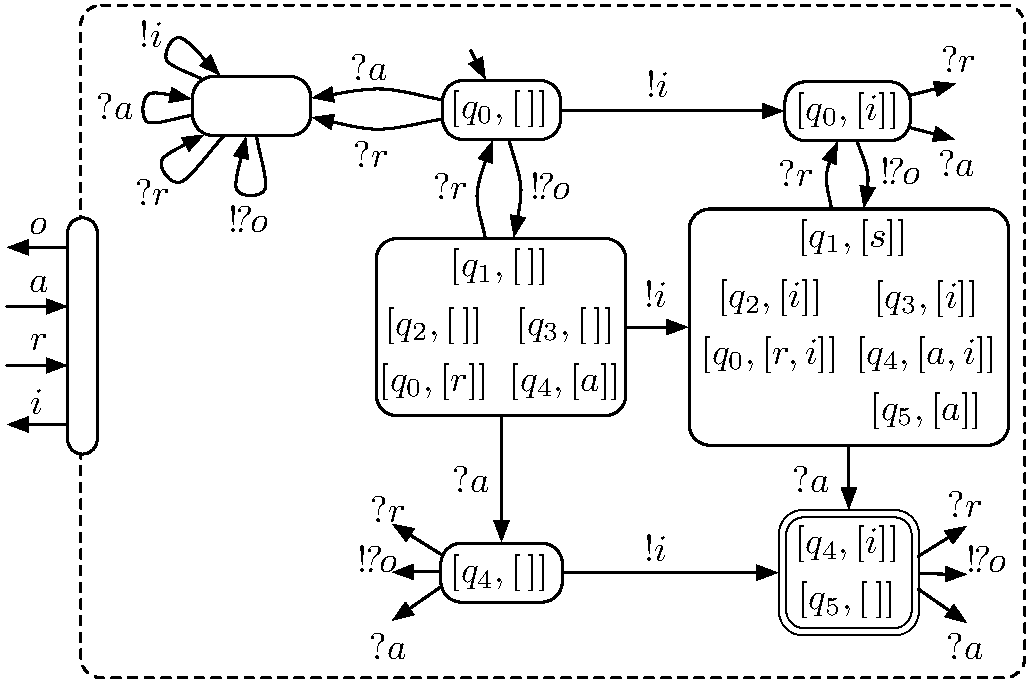
\includegraphics[scale=0.45]{background/running_mpp}
\caption{The synthesized strategy $\TS_{1}(A_\text{Buy})$ of the buyer service $A_\text{Buy}$ from \autoref{fig:Abuy} for $k=1$. Transitions without target states are assumed to have the state $\emptyset\in 2^{Q\times\Bags(\M_{a})}$ as target.}
\label{fig:mpp}
\end{figure}





%%%%%%%%%%%%%%%%%%%%%%%%%%%%%%%%%%%%%%%%%%%%%%%%%%%%%%%%%%%%%%%%%%%%%%%%%%%%%%%
\section{Finite characterization of strategies}
%%%%%%%%%%%%%%%%%%%%%%%%%%%%%%%%%%%%%%%%%%%%%%%%%%%%%%%%%%%%%%%%%%%%%%%%%%%%%%%

In this section, we summarize results from Massuthe and Wolf~\cite{LohmannMW_2007_atpn,Massuthe_2009_phd} to finitely characterize the possibly infinite set of strategies of a service. As a first observation, strategies can be compared with each other with respect to their behavior. In particular, some strategies permit ``more behavior'' than others.

%%%%%%%%%%%%%%%%%%%%%%%%%%%%%%%%%%%%%%%%%%%%%%%%%%%%%%%%%%%%%%%%%%%%%%%%%%%%%%%
\begin{definition}{\boldmath$k$-most-permissive strategy}
\label{def:mps}%
A strategy $B^*\in\Strat_{k}(A)$ of a service automaton $A$ is \define{$k$-most-permissive} iff $B^*$ structurally matches any other $k$-strategy of~$A$.
\end{definition}
%%%%%%%%%%%%%%%%%%%%%%%%%%%%%%%%%%%%%%%%%%%%%%%%%%%%%%%%%%%%%%%%%%%%%%%%%%%%%%%

Thereby, the structural matching relation between service automata is defined on their underlying labeled transition systems. A most-permissive strategy can be seen as a top element in a preorder of service behaviors. This preorder~\cite{Massuthe_2009_phd} is out of scope of this thesis. The strategy synthesized by the algorithm of~\autoref{def:synthesis} is a most-permissive strategy.

%%%%%%%%%%%%%%%%%%%%%%%%%%%%%%%%%%%%%%%%%%%%%%%%%%%%%%%%%%%%%%%%%%%%%%%%%%%%%%%
\begin{proposition}{Synthesis is most-permissive~\cite{Wolf_2008_topnoc}}
Let $A$ be a $k$-controllable service automaton.\\ Then $\TS_{k}(A)$ is a $k$-most-permissive strategy of $A$.\label{prop:mostpermissivestrategy}
\end{proposition}
%%%%%%%%%%%%%%%%%%%%%%%%%%%%%%%%%%%%%%%%%%%%%%%%%%%%%%%%%%%%%%%%%%%%%%%%%%%%%%%

The proof~\cite{LohmannMW_2007_atpn,Wolf_2008_topnoc,Massuthe_2009_phd} is based on \autoref{thm:strategy} and exploits that the composition with any service automaton with ``more'' behavior would not be compatible.

By definition, a $k$-most-permissive strategy $B^*$ of a $k$-controllable service $A$ structurally matches any other $k$-strategy of $A$. The converse does, however, not hold: there exist service automata $C\notin\Strat_{k}(A)$ which are structurally matched by $B^*$. Such services can be ruled out by adding Boolean annotations to the states of a $B^*$.

%%%%%%%%%%%%%%%%%%%%%%%%%%%%%%%%%%%%%%%%%%%%%%%%%%%%%%%%%%%%%%%%%%%%%%%%%%%%%%%
\begin{definition}{Annotated automaton}
\nomenclature[BPhi]{$B^{\varphi}=[B,\varphi]$}{an annotated automaton}%
\nomenclature[final]{$\final$}{proposition that evaluates to true in a final state}%
\nomenclature{$\wedge$}{Boolean conjunction}%
\nomenclature{$\vee$}{Boolean disjunction}%
\nomenclature{$\neg$}{Boolean negation}%
The tuple $B^{\varphi}=[B,\varphi]$ is an \define{annotated automaton} iff $B=[Q,q_{0},{\shortrightarrow},\{P\}]$ is a deterministic $\tau$-free single-port service automaton without final states, and $\varphi$ is an annotation that assigns a Boolean formula to every state $q\in Q$. The formulae are built on $\E_{P}$, an additional proposition $\final$, and the Boolean operators $\wedge$, $\vee$, and $\neg$.
\end{definition}
%%%%%%%%%%%%%%%%%%%%%%%%%%%%%%%%%%%%%%%%%%%%%%%%%%%%%%%%%%%%%%%%%%%%%%%%%%%%%%%

Annotated automata have been introduced by \citet{WombacherFMN_2004_ijwsr} to represent sets of automata. In our context, the Boolean formulae are used to refine the structural matching relation by adding constraints on the edges that leave a state of a service automaton that is structurally matched by a most-permissive partner. Annotated automata have no final states; whether a state of a represented automaton needs to be final is expressed by the proposition $\final$. The truth value of an annotated formula is evaluated by an assignment function.

%%%%%%%%%%%%%%%%%%%%%%%%%%%%%%%%%%%%%%%%%%%%%%%%%%%%%%%%%%%%%%%%%%%%%%%%%%%%%%%
\begin{definition}{Assignment, model}
\nomenclature[b]{$\beta$, $\beta'$}{assignment functions}%
\nomenclature[p]{$\varphi$}{a Boolean formula}%
\label{def:assignment}%
Let $A=[Q,q_{0},{\shortrightarrow},\Omega,\mathcal{P}]$ be a service automaton. We define the \define{assignment} $\beta:Q\times(\E\cup\{\final\})\rightarrow\{\mathit{true},\mathit{false}\}$ as follows:
$$\beta(q,p):=\begin{cases}
\mathit{true}\text{,}&\text{if $p\in \lab^*(q)$,}\\
\mathit{true}\text{,}&\text{if $p=\final$ and $\tau(q)\cap \Omega\neq\emptyset$,}\\
\mathit{false}\text{,}&\text{otherwise}.
\end{cases}$$
A state $q\in Q$ \define{models} a formula $\varphi$ (denoted $q\models\varphi$) iff $\varphi$ evaluates to $\mathit{true}$ under the assignment $\beta(q,\varphi)$. We thereby assume the standard semantics for the Boolean operators $\wedge$, $\vee$, and $\neg$.
\end{definition}
%%%%%%%%%%%%%%%%%%%%%%%%%%%%%%%%%%%%%%%%%%%%%%%%%%%%%%%%%%%%%%%%%%%%%%%%%%%%%%%

An atomic proposition of a formula is true in a state of a service automaton if that state has a respective outgoing edge, possibly reached by a sequence of internal steps. The proposition $\final$ is evaluated to true exactly in final states. The following definition of \emph{matching} combines structural matching and formulae evaluation.

%%%%%%%%%%%%%%%%%%%%%%%%%%%%%%%%%%%%%%%%%%%%%%%%%%%%%%%%%%%%%%%%%%%%%%%%%%%%%%%
\begin{definition}{Matching}\label{def:matching}%
\nomenclature[Match]{$\Match(B^{\varphi})$}{the set of service automata that match with $B^{\varphi}$}%
A service automaton $A$ \define{matches} with an annotated automaton $B^{\varphi}$ iff:
\begin{myenumerate}
\item there exists a structural matching relation $\varrho\subseteq Q_{A}\times Q_{B}$ and
\item for all $[q_{A},q_{B}]\in\varrho$: $q_{A} \models \varphi(q_{B})$.
\end{myenumerate}
Let $\Match(B^{\varphi})$ denote the set of service automata that match with~$B^{\varphi}$.
\end{definition}
%%%%%%%%%%%%%%%%%%%%%%%%%%%%%%%%%%%%%%%%%%%%%%%%%%%%%%%%%%%%%%%%%%%%%%%%%%%%%%%

The first requirement states that a service automaton matches with an annotated automaton only if there exists a structural matching relation. If such a relation exists, it consists of pairs of states for which the formulae must be satisfied in the second step. With this matching predicate, an annotated automaton implicitly defines a (possibly infinite) set of service automata. In particular, we are interested in annotated  automata that exactly characterize the set of $k$-strategies of a service.

%%%%%%%%%%%%%%%%%%%%%%%%%%%%%%%%%%%%%%%%%%%%%%%%%%%%%%%%%%%%%%%%%%%%%%%%%%%%%%%
\begin{definition}{\boldmath$k$-operating guideline}%
\nomenclature[OGkA]{$\OG^k_{A}$}{a $k$-operating guideline of $A$}%
A \define{$k$-operating guideline} for a service automaton $A$ is an annotated automaton\break $\OG^k_{A}=B^\varphi$ such that $\Match(\OG^k_{A})=\Strat_{k}(A)$.
\end{definition}
%%%%%%%%%%%%%%%%%%%%%%%%%%%%%%%%%%%%%%%%%%%%%%%%%%%%%%%%%%%%%%%%%%%%%%%%%%%%%%%

Every $k$-controllable service has a $k$-operating guideline; Masuthe et~al.~\cite{LohmannMW_2007_atpn,Massuthe_2009_phd} provide detailed proofs and a construction algorithm. The core idea is to use a $k$-most-permissive strategy and to annotate each state with a formula that is satisfiable iff those events are present that resolve any deadlock within the associated closure of states while still respecting the message bound.

Beside the aforementioned finiteness, Massuthe and Wolf~\cite{LohmannMW_2007_atpn,Massuthe_2009_phd} further emphasize the following properties that operating guidelines enjoy. These properties are essential for the results we present in subsequent chapters.
\begin{niceitemize}
\item Matching is only defined in terms of structurally matching and formula evaluation. In particular, it does not take the states of the closure (cf.~\autoref{def:closure}) into account. This not only allow for a compact representation (\ie,~only the structure of a most-permissive partner needs to be stored), but also avoids an explicit exposure of the service's internal structure which might be subject to trade secrets.
\item The formulae of an operating guideline can be transformed into positive formulae (\ie,~formulae without negations)~\cite{LohmannW_2009_acsd}. This increases the efficiency of formula evaluation during matching.
\item Having a most-permissive strategy as structure, operating guidelines are operational; that is, $k$-compatible service automata can be easily derived from operating guidelines.
\end{niceitemize}

\medskip

Operating guidelines defined in~\cite{LohmannMW_2007_atpn,Massuthe_2009_phd} base on a compatibility notion that does not include responsiveness. To this end, operating guidelines also characterize services that ``control'' other services by performing an infinite sequence of noncommunicating actions (\eg, $\tau$-loops). Even if the interaction with such unresponsive services is deadlock free and bounded, these services can hardly be used to construct compatible service compositions. Therefore, Defs.~\ref{def:synthesis}--\ref{def:matching} have been adjusted to be applicable in the context of our compatibility criterion.

\paragraph{Example.} \Autoref{fig:og} depicts an operating guideline of the seller service. It has the structure of the most-permissive strategy of \autoref{fig:mpp} and each state is annotated with a Boolean formulae. These formulae constrain the behavior of matching services. For instance, formula ${?a}\wedge{?r}$ demands that a matching service must be able to receive an acceptance~($a$) \emph{and} a rejection ($r$) message. The state modeling unreachable behavior is annotated with \emph{true}: we pose no constraints on unreachable behavior. Note that the events that lead to this \emph{true}-annotated state (\eg, $?a$ and~$?r$ in the initial state) are not mentioned in the formulae.

%%%%%%%%%%%%%%%%%%%%%%%%%%%%%%%%%%%%%%%%%%%%%%%%%%%%%%%%%%%%%%%%%%%%%%%%%%%%%%
\begin{figure}
\centering
\subfigure[$\OG^{1}_{A_\text{Buy}}$\label{fig:og}]{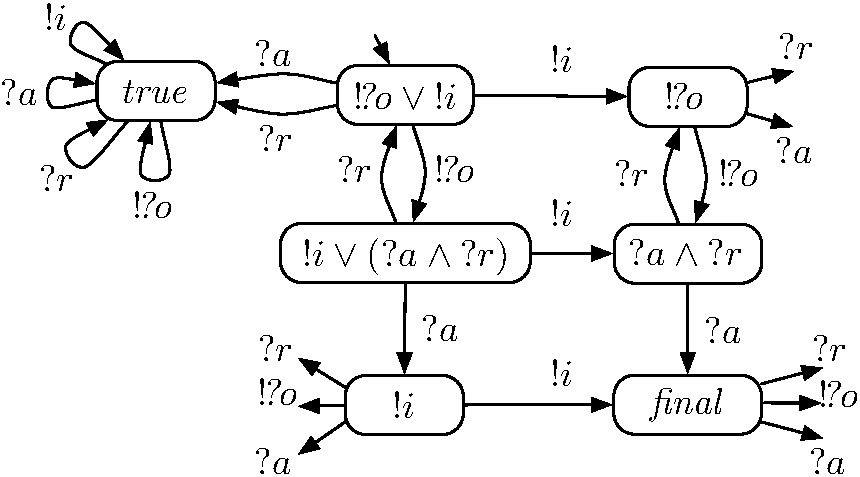
\includegraphics[scale=0.45]{background/running_og}}\hfill
\subfigure[matching with $\OG^{1}_{A_\text{Buy}}$\label{fig:match}]{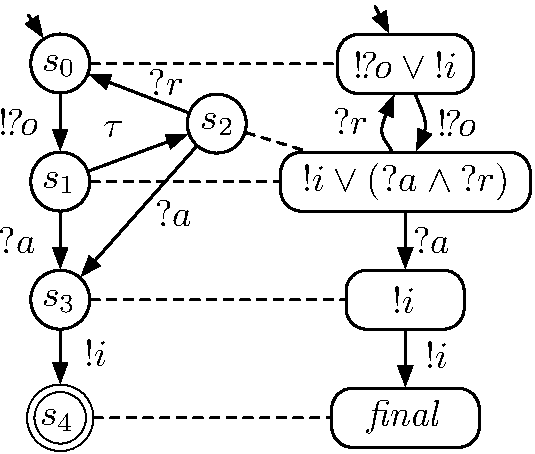
\includegraphics[scale=0.45]{background/running_matching}}
\caption{The operating guideline $\OG^{1}_{A_\text{Buy}}$ (a) of the buyer service $A_\text{Buy}$. Transitions without target states are assumed to have the state with the ``\emph{true}'' annotation as target. A matching service automaton together with the structural matching relation is depicted in (b).}
\end{figure}
%%%%%%%%%%%%%%%%%%%%%%%%%%%%%%%%%%%%%%%%%%%%%%%%%%%%%%%%%%%%%%%%%%%%%%%%%%%%%%

\Autoref{fig:match} depicts an example for a matching service. The dashed lines connect states that are in a structural matching relation between a seller service and a fraction of $\OG^{1}_{A_\text{Buy}}$. The states $s_{1}$ and $s_{2}$ are connected by a $\tau$-annotated edge and match with the same state in the operating guideline. State $s_{1}$ satisfies the formula ${!i}\vee({?a}\wedge{?r})$, because the state $s_{2}$ has both an edge labeled with ${?a}$ and ${?r}$, and this state is internally reachable from $s_{1}$.





%%%%%%%%%%%%%%%%%%%%%%%%%%%%%%%%%%%%%%%%%%%%%%%%%%%%%%%%%%%%%%%%%%%%%%%%%%%%%%%
\section{Experimental Results}\label{sect:background:experiment}
%%%%%%%%%%%%%%%%%%%%%%%%%%%%%%%%%%%%%%%%%%%%%%%%%%%%%%%%%%%%%%%%%%%%%%%%%%%%%%%

Both the strategy synthesis algorithm~\cite{Wolf_2008_topnoc} (cf.\ \autoref{def:synthesis}) and the algorithm to calculate an operating guideline for a service~\cite{LohmannMW_2007_atpn,Massuthe_2009_phd} have been implemented in the tool Wendy~\cite{LohmannW_2009_wendy}. These two algorithms were originally implemented in the tool Fiona~\cite{MassutheW_2008_awpn}. The design goal of Fiona was the combination of several analysis and synthesis algorithms for service behavior. This is reflected by a flexible architecture that aims at the reusability of data structures and algorithms. Although this design facilitated the quick integration and validation of new algorithms, the growing complexity made optimizations more and more complicated.

To overcome these efficiency problems, Wendy is a reimplementation of the two synthesis algorithms as compact single-purpose tool. This reimplementation incorporates the experiments made by analyzing performance bottlenecks through improved data structures and memory management, validation of experimental results which gave a deeper understanding of the parameters of the models that affect scalability, and theoretical observations on regularities of synthesized strategies and operating guidelines.

As a proof of concept, we calculated operating guidelines of several \acronym{WS-BPEL} services from a consulting company. Each process consists around 40 \acronym{WS-BPEL} activities and models communication protocols and business processes of different industrial sectors. To apply the algorithms of this chapter, we first translated the \acronym{WS-BPEL} processes into service automata using the compiler \bpelowfn{}~\cite{Lohmann_2007_hubtr212} implementing the formal semantics we shall discuss in \autoref{chap:verification}.

%%%%%%%%%%%%%%%%%%%%%%%%%%%%%%%%%%%%%%%%%%%%%%%%%%%%%%%%%%%%%%%%%%%%%%%%%%%%%%
\begin{table}
\centering
\caption{Experimental results for strategy synthesis using Wendy.}
\medskip
\label{tab:synthesis}
\footnotesize
\begin{tabular*}{\textwidth}{@{\extracolsep{\fill}}lrrcrrr}
\toprule
& \multicolumn{3}{c}{analyzed service automaton} & \multicolumn{3}{c}{synthesis result} \\ 
service & \multicolumn{1}{c}{$|Q|$} & \multicolumn{1}{c}{$|{\shortrightarrow}|$} & $|\E_{\mathcal{P}}|$ & \multicolumn{1}{c}{$|Q_{\TS}|$} & \multicolumn{1}{c}{$|{\shortrightarrow}_{\TS}|$} & \multicolumn{1}{c}{time (sec)} \\ \midrule
Quotation &            $602$ &      $1{,}141$ & $19$ & $11{,}264$ & $145{,}811$ &   $0$ \\
Deliver goods &       $4{,}148$ & $13{,}832$ & $14$ &  $1{,}376$ &  $13{,}838$ &   $2$ \\ %daniela
{\scriptsize SMTP} protocol &     $8{,}345$ & $34{,}941$ & $12$ & $20{,}818$ & $144{,}940$ &  $29$ \\ %-m3
Car analysis &     $11{,}381$ & $39{,}865$ & $15$ &  $1{,}448$ &  $13{,}863$ &  $49$ \\ %daniela
Identity card &      $14{,}569$ & $71{,}332$  & $11$ &  $1{,}536$ &  $15{,}115$ & $82$ \\
Product order &     $14{,}990$ & $50{,}193$ & $16$ & $57{,}996$ & $691{,}414$ & $294$ \\ %-m2
\bottomrule
\end{tabular*}
\end{table}
%%%%%%%%%%%%%%%%%%%%%%%%%%%%%%%%%%%%%%%%%%%%%%%%%%%%%%%%%%%%%%%%%%%%%%%%%%%%%%

\Autoref{tab:synthesis} lists details on the processes as well as the experimental results. We see that the service automata derived from the \acronym{WS-BPEL} processes have up to 14{,}990 states. These large sizes can be explained by the fact that both the positive as well as the negative control flow (\ie, fault and compensation handling) are modeled. The interfaces consist of up to 19 \acronym{WSDL}~\cite{standard_wsdl} operations.

%%%%%%%%%%%%%%%%%%%%%%%%%%%%%%%%%%%%%%%%%%%%%%%%%%%%%%%%%%%%%%%%%%%%%%%%%%%%%%
\begin{figure}[t!]
\centering
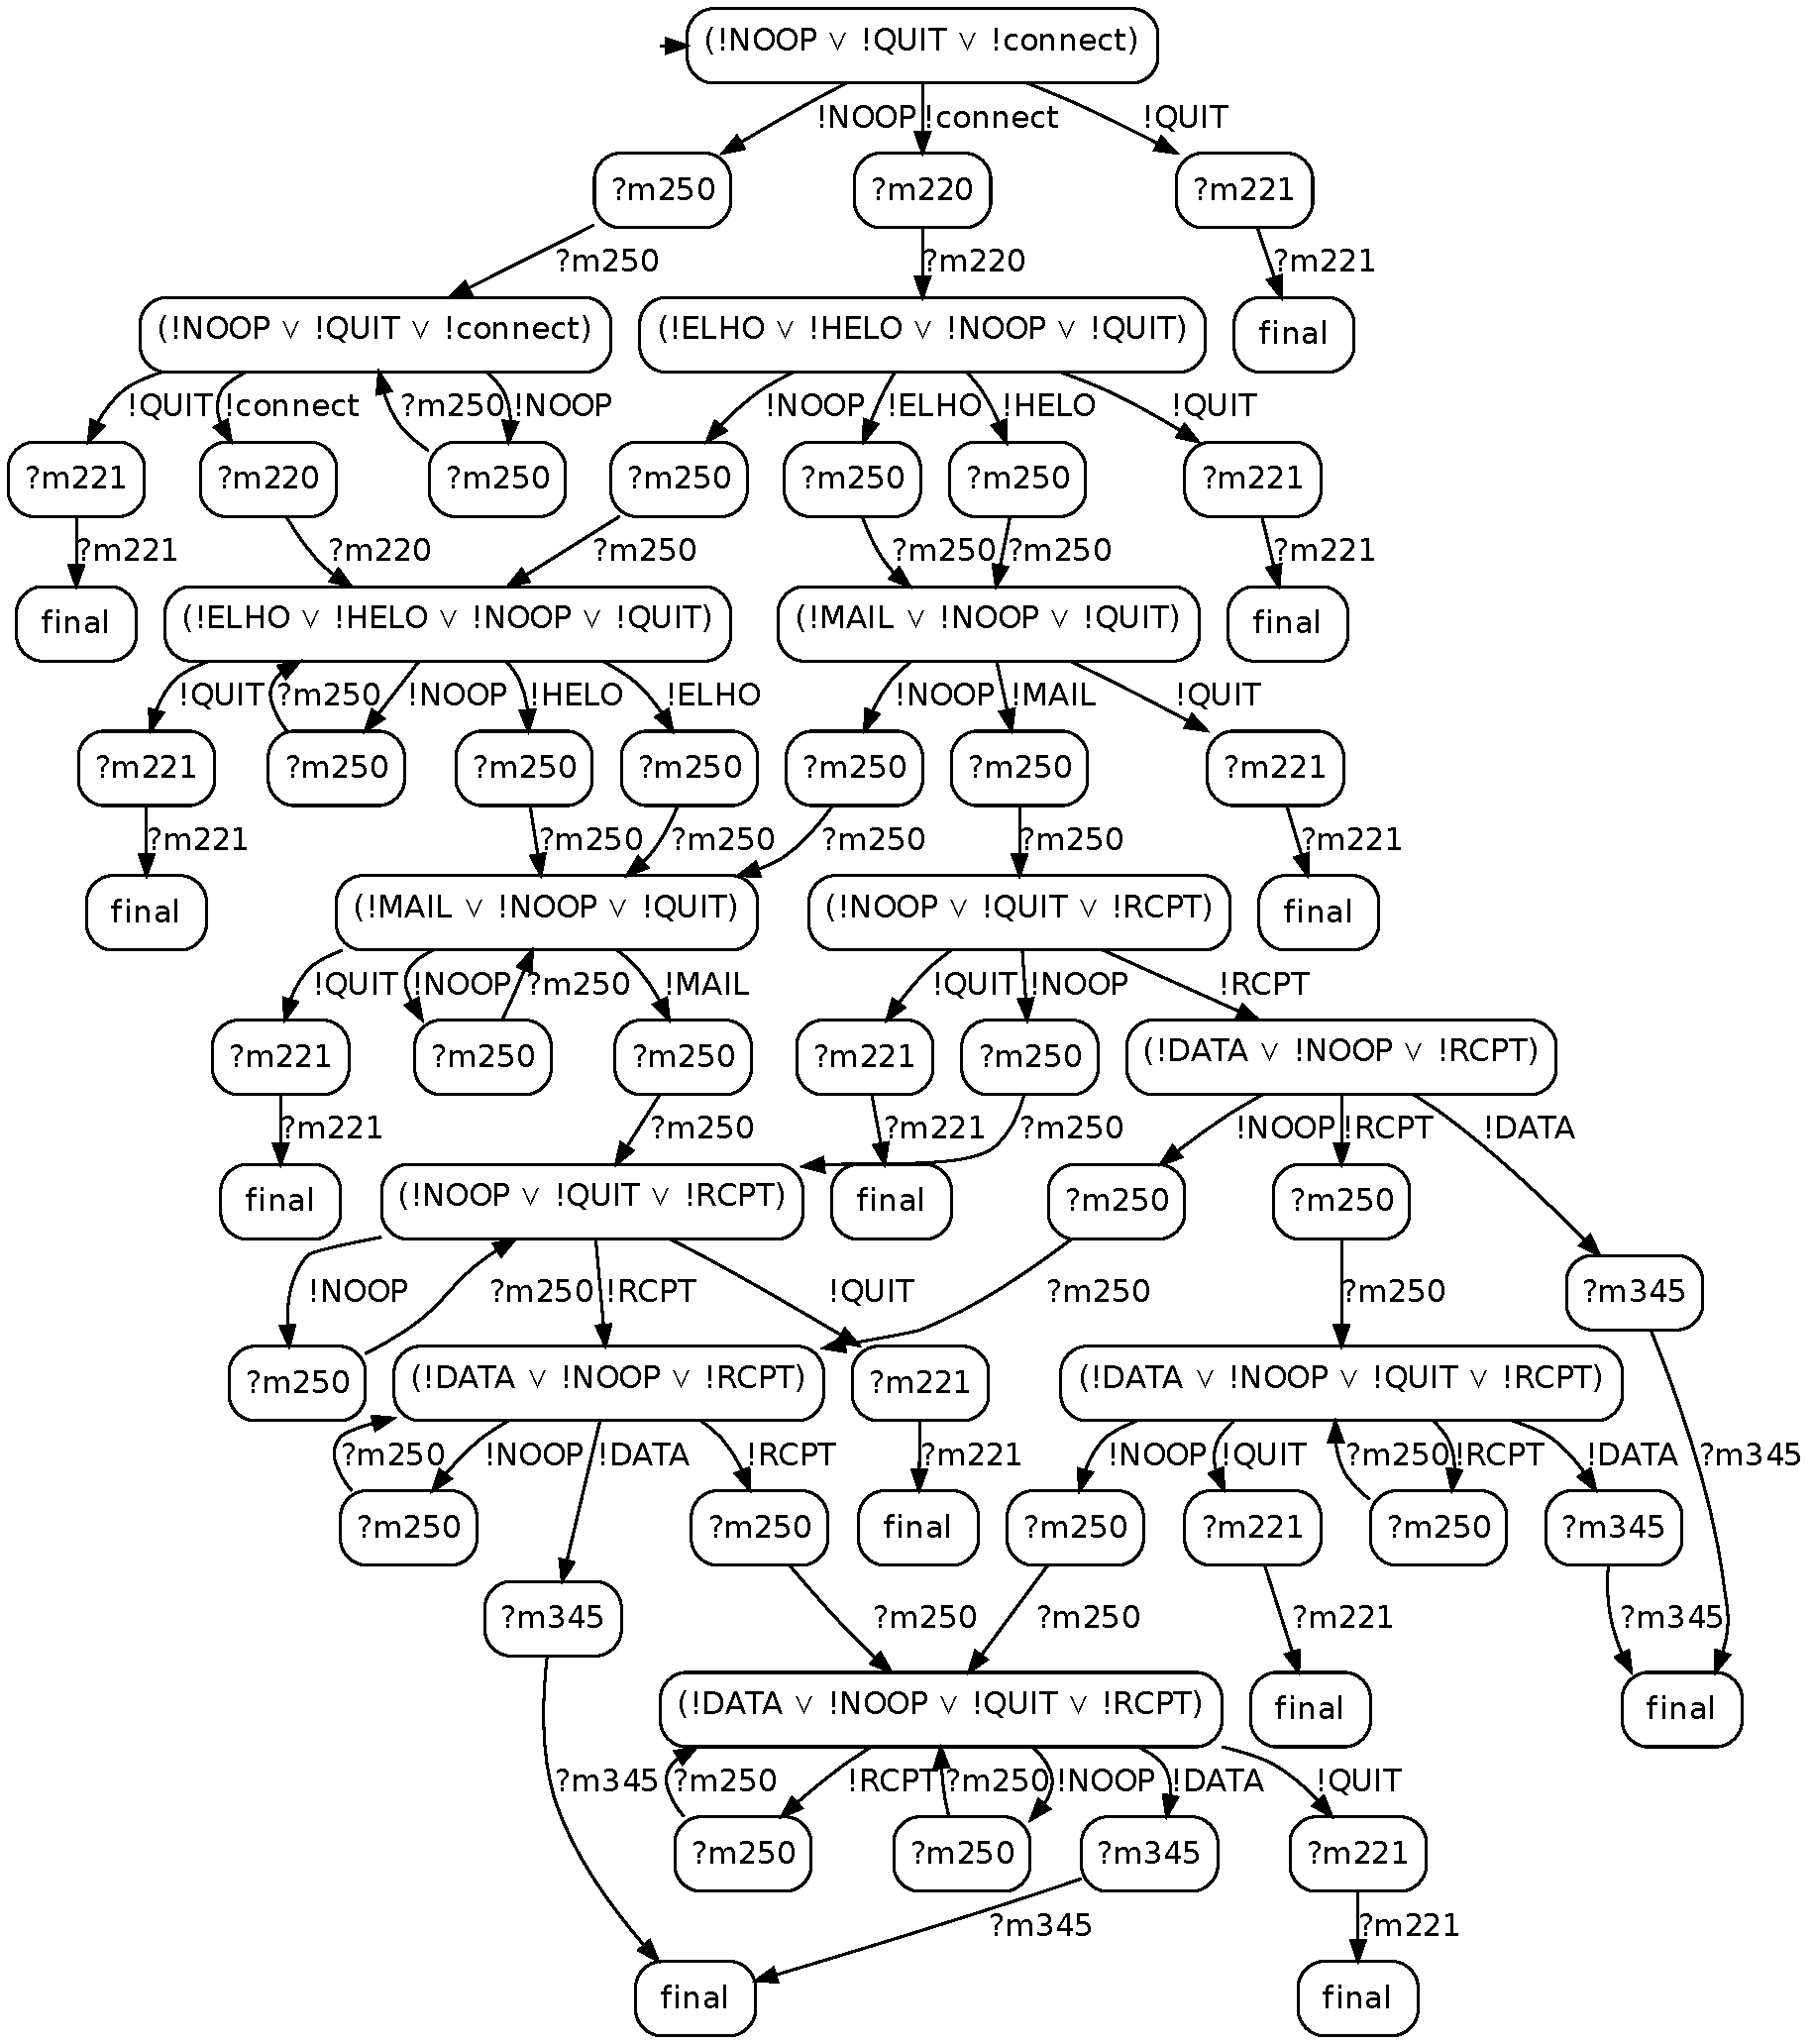
\includegraphics[width=0.9\textwidth]{background/smtp}
\caption{Operating guideline for the \acronym{SMTP} protocol (reduced version) as calculated by the tool Wendy.}\label{fig:smtp}
\end{figure}
%%%%%%%%%%%%%%%%%%%%%%%%%%%%%%%%%%%%%%%%%%%%%%%%%%%%%%%%%%%%%%%%%%%%%%%%%%%%%%


The number of states of the operating guidelines (\ie, the most-permissive strategy) are sometimes much larger than the original service. The number of transitions grows even faster. From these transitions, about the moiety have the empty node $q=\emptyset$ as target state. The analysis takes up to 294 seconds on a 3 \acronym{GH}z computer. This is acceptable, because operating guidelines are usually calculated to be used by the service broker many times. \citet{Massuthe_2009_phd} reports an experiment where the compatibility of two services $A$ and $B$ is verified by model checking the composition $A\oplus B$ on the one hand and calculating the operating guideline $\OG_{A}$ and checking whether $B\in\Match(\OG_{A})$ on the other hand. As result, Massuthe reports that using operating guidelines outperforms model checking in case more than seven checks are made.

In comparison, Fiona could only analyze three of the six services without exceeding 2 \acronym{GB} of memory. For the other models, the analysis was between 5 and 70 times slower than Wendy. To conclude, Wendy allows for the synthesis of strategies and the calculation of operating guidelines of industrial Web services. To give an example of the structure of such strategies, \autoref{fig:smtp} shows an operating guideline of a smaller version of the \acronym{SMTP} protocol.






%%%%%%%%%%%%%%%%%%%%%%%%%%%%%%%%%%%%%%%%%%%%%%%%%%%%%%%%%%%%%%%%%%%%%%%%%%%%%%%
\section{Discussion}
\label{chap:background:discussion}
%%%%%%%%%%%%%%%%%%%%%%%%%%%%%%%%%%%%%%%%%%%%%%%%%%%%%%%%%%%%%%%%%%%%%%%%%%%%%%%

The original contribution of this chapter is the definition of \emph{service automata as a unified formalism to define and reason about services and service compositions that communicate synchronously or asynchronously}. We conclude this chapter with a discussion and a classification of service automata. A discussion of controllability and operating guidelines is beyond the scope of this theses, and we refer the interested reader to the work of Massuthe et al.~\cite{LohmannMW_2007_atpn,Wolf_2008_topnoc,Massuthe_2009_phd}.

\medskip

Communication protocols have been studied and formalized long before the advent of service orientation~\cite{Merlin_1979_ieeesoc,BochmannS_1980_ieeetoc}. Such a formalization must on the one hand specify the protocol or \emph{control flow} itself (\ie,~the order in which messages are exchanged) and the underlying \emph{communication model} (\ie,~the way messages are transfered) on the other hand. Prominent control flow models are finite automata~\cite{HopcroftMU_1979}, Petri nets~\cite{Reisig_1985}, and process algebras~\cite{Baeten_2005_tcs}. As communication model, usually a choice is made between either synchronous or asynchronous message transfer.

We first justify our choice for an automaton-based model for the control flow. This choice is motivated by the correctness criteria that are studied in this thesis: compatibility, controllability, and realizability (cf.~\autoref{chap:realizability}) are \emph{behavioral} criteria defined in terms of states and runs of services and their composition rather than on their structure. Structural approaches, which avoid a state space exploration, are usually defined for special subclasses (\eg,~soundness checks for free-choice Petri nets~\cite{VerbeekBA_2001_tcj}), or allow only for the definition of either necessary \emph{or} sufficient criteria (\eg,~compatibility criteria derived from the state equation~\cite{OaneaW_2009_zeus}). Furthermore, the algorithms to synthesize strategies and operating guidelines are based on states. To this end, we decided to use a formalism with an explicit notion of states rather than models with an implicit notion of states, such as Petri nets or process algebras. This decision also takes into account that none of the algorithms presented in this thesis currently exploits the ability of Petri nets and process algebras to explicitly express concurrency. Nevertheless, Petri~nets can be later used to compactly represent service automata and operating guidelines~\cite{LohmannW_2009_acsd}.

Service automata are introduced as a uniform instrument to \emph{reason} about correctness of services rather than to \emph{model} services. To create models of services, domain-specific languages, such as \acronym{BPMN} or \acronym{WS-BPEL}, and graphical formalisms, such as Petri nets or \acronym{MSC}s, are far more accessible to domain experts. Such models can, however, be easily translated into service automata:  \citet{Massuthe_2009_phd} presents a bidirectional translation between open nets and service automata, and there exists a variety of translations~\cite{BreugelK2006,LohmannVOSA_2009_ijbpim,LohmannVD_2008_topnoc} of service description languages into Petri nets and other formalisms related to automata.

\citet{KazhamiakinPS_2006_www} compare the expressiveness of different communication models with respect to their ability to detect errors in service compositions. They define a parametrized \emph{state transition system with channels}. Depending on the parameters on numbers, sizes, and ordering abilities of the channels, they constitute a hierarchy of communication models and discuss the tradeoff between expressiveness and analysis performance.

The most restricted communication model is synchronous communication. It allows for simple models and efficient verification, but makes strong assumptions on the underlying infrastructure implementing the message exchange between the services. In particular, the whole message transfer is considered to be instantaneous. Formalisms using synchronous communications include service automata, \emph{I/O automata}~\cite{Lynch_1996}, \emph{interface automata}~\cite{AlfaroH_2001_fse}, the ``Roman Model''~\cite{BerardiCGLM_2003_icsoc}, and \emph{message exchanging finite state automata}~\cite{BaldoniBMP_2006_icsoc}. Synchronous communication is also  common in interaction models, for instance \emph{interaction Petri nets}~\cite{DeckerW_2007_bpm}. \citet{Wolf_2007_sa} and \citet{Wolf_2008_topnoc} study Petri net models in which multiple synchronous events may occur simultaneously. This extension has an impact on compatibility and controllability, because a set of simultaneously occurring synchronous events can reach different states than an arbitrary interleaving of these events. Due to increased verification complexity and little practical relevance, we decided not to extend our communication model this way.

A more general communication model decouples the sending and the receiving of a message, but still assumes that the order of sending messages implies an order in which these messages are received; that is, messages are not reordered during communication. This is typically modeled by \acronym{FIFO} queues. Decidability issues in the context of unbounded queues were studied with \emph{communicating finite state machines}~\cite{BrandZ_1983_jacm}, and recent work employing \acronym{FIFO} queues usually assume a finite bound~\cite{FuBS_2004_www,FuBS_2005_tse}, sometimes even fixed to the size of one~\cite{BalbianiCF_2008_ieeeservice,BerardiCGHM_2005_vldb}.

Finally, the most general communication model assumes unordered message buffers which can be modeled using multisets. Beside service automata, \emph{concurrent automata}~\cite{AlurEY_2003_tse} and \emph{open nets}~\cite{KindlerMR_2000_bpm,Kindler_1997_atpn,Martens_2003_phd,ReisigSS_2005_ife,MassutheRS_2005_amct} follow this approach in which no assumptions are made about the infrastructure other than messages not to get lost.

\citet{BultanFHS_2003_www} stress that the verification of asynchronous communication is more complex than synchronous communication. To this end, \citet{FuBS_2005_tse} examine under which conditions asynchronous communication can be safely abstracted to synchronous communication. They provide sufficient conditions which include the strong requirement that at most one message event is activated in every reachable state of a composition. We investigated the impact of communication models to controllability~\cite{Lohmann_2010_zeus} and showed that small variations in the communication model (\eg, changing the message bound) can make controllable services uncontrollable, and vice versa.

\medskip

To conclude, service automata support \emph{both} synchronous and (unordered) asynchronous communication and hence cover the entire range of the communication model hierarchy~\cite{KazhamiakinPS_2006_www}. The ability to mix synchronous and asynchronous communication (similar to \cite{Wolf_2007_sa,BultanF_2008_soca,Wolf_2008_topnoc}) allows us to faithfully represent and reason about service models at different levels of abstraction.


\part{Correctness of Services}\label{part1}
\chapter{Validation and selection}%
\label{chap:validation}%
\chapintro{This chapter is based on results published in~\cite{LohmannMW_2007_bpm}.}


\lettrine[findent=.2em,lines=2,nindent=0pt]{I}{n} this chapter, we investigate the set of strategies of a controllable service. Although each strategy models a correct interaction, not every strategy is \emph{intended} in practice. We shall provide means to express intended and unintended behavior as \emph{behavioral constraints}. With such constraints, the set of strategies can be ``filtered'', and the remaining strategies can be used in several applications from service validation to service discovery. In \autoref{sect:validation_sa} and \autoref{sect:validation_og}, we show how constraints can be applied to service automata and operating guidelines, respectively. First experiences with implementations of behavioral constraints are reported in \autoref{sect:validation_implementation}. Finally, we discuss related work and give a conclusion.

\nomenclature[Prov]{$\Prov$}{a provider service}%
\nomenclature[Req]{$\Req$}{a requestor service}%
We motivate, define, and discuss behavioral constraints in the context of service-oriented architectures (\acronym{SOA}). To explain the different scenarios, we distinguish a service provider with a service $\Prov$, a service requestor with a service $\Req$, and a service broker, which maintains a registry of several provider services (cf.~\autoref{fig:soatriangle}). The definitions of this chapter are, however, independent of these roles and are applicable to any setting in which services communicate.





%%%%%%%%%%%%%%%%%%%%%%%%%%%%%%%%%%%%%%%%%%%%%%%%%%%%%%%%%%%%%%%%%%%%%%%%%%%%%%%
\section{Intended and unintended behavior}
%%%%%%%%%%%%%%%%%%%%%%%%%%%%%%%%%%%%%%%%%%%%%%%%%%%%%%%%%%%%%%%%%%%%%%%%%%%%%%%

In \autoref{chap:formal}, we introduced the notion of controllability as a fundamental correctness criterion for services. A controllable provider service $\Prov$ is correct in the sense that there exists at least one strategy (\ie, a requestor service $\Req$) such that their composition is compatible. With operating guidelines, the set of all strategies (\ie, all requestor services) can be characterized. In addition, compatible requestor service automata can be generated from this operating guideline.

In practice, the sole existence of an arbitrary strategy may be a too coarse correctness notion, because there usually exist \emph{intended} and \emph{unintended} strategies. Consider for example the buyer service from the previous chapter. After an update of its functionality, it might introduce the possibility to cancel ($c$) the negotiation at any time. \Autoref{valdiation:fig:running} depicts this updated buyer service and \autoref{valdiation:fig:runningog} shows the operating guideline of this service. To increase legibility, we refrained from drawing the empty node $q=\emptyset$. The operating guideline now also characterizes sellers that cancel after each step of the negotiation. These interactions with canceling sellers (cf.~\autoref{validation:fig:unintended}) are still compatible. However, the owner of the buyer service is rather interested whether it is still possible to actually buy goods. A filtered operating guideline that only characterizes selling\,---\,and hence intended\,---\,customers would be helpful in this setting.

%%%%%%%%%%%%%%%%%%%%%%%%%%%%%%%%%%%%%%%%%%%%%%%%%%%%%%%%%%%%%%%%%%%%%%%%%%%%%%
\begin{figure}
\centering
{}\hfill
\subfigure[$A_{\text{Buy}}^{*}$\label{valdiation:fig:running}]{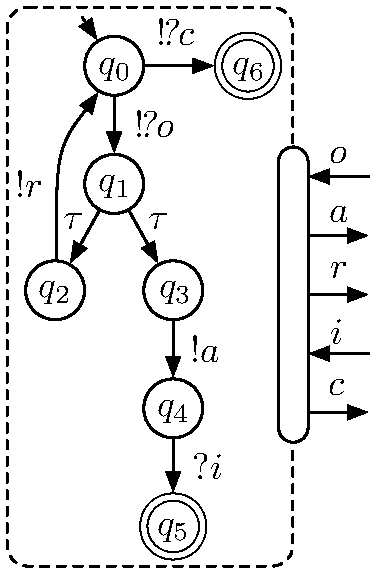
\includegraphics[scale=0.45]{validation/running-cancel}}\hfill
\subfigure[$A_{\text{Cancel}}$\label{validation:fig:unintended}]{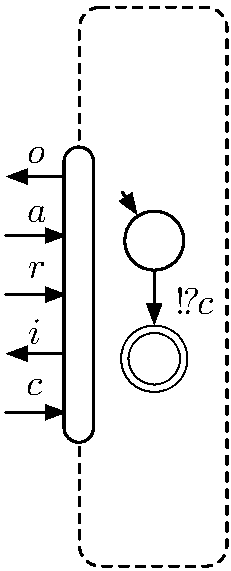
\includegraphics[scale=0.45]{validation/running-bad}}\hfill ${}$
\subfigure[$\OG^{1}_{A_{\text{Buy}}^{*}}$\label{valdiation:fig:runningog}]{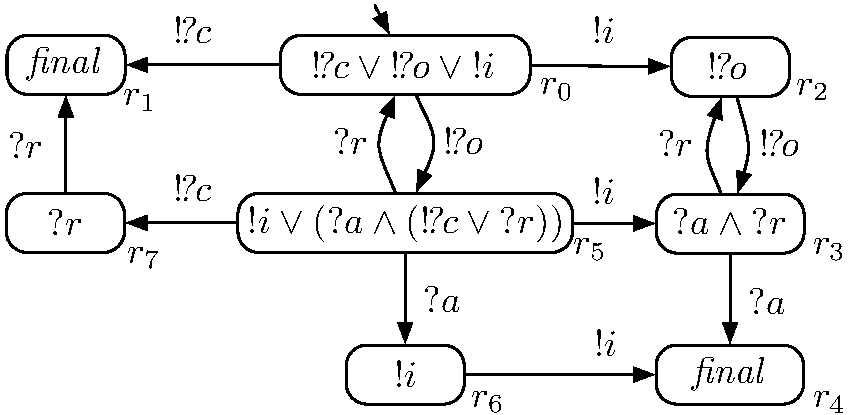
\includegraphics[scale=0.45]{validation/running-cancel-og}}
\caption{Adjusted buyer service (a) with operating guideline (c) and compatible seller service that always cancels (b).}
\label{validation:fig:buyer2}
\end{figure}
%%%%%%%%%%%%%%%%%%%%%%%%%%%%%%%%%%%%%%%%%%%%%%%%%%%%%%%%%%%%%%%%%%%%%%%%%%%%%%

Another evaluation of strategies may stem from the owner of a service registry: A service broker might classify provider services as intended or unintended. For example, he may want to ensure certain features for registered services, such as payment only with certain credit cards. Finally, a client requesting the registry might be interested in services implementing a certain protocol. For instance, he could prefer arranged communication such that certain actions occur in a given order (\emph{first} accepting terms of payment and \emph{then} sending a booking confirmation, for instance).

In the remainder of this chapter, we study \emph{behavioral constraints} (constraints for short) that have to be satisfied in addition to compatibility. We provide a formal approach for steering the communication with a service $\Prov$ into a desired direction and also constrain operating guidelines. A~constrained operating guideline of a service $\Prov$ characterizes all those services $\Req$ such that $\Req\oplus \Prov$ is compatible \emph{and} satisfies a given constraint. Technically, a behavioral constraint expresses a criterion that is used to restrict the set $\Strat(\Prov)$ of strategies of the service $\Prov$.

We identify four scenarios involving behavioral constraints.

\begin{niceenumerate}
\item \emph{Validation}. Before deploying a service $\Prov$ or publishing it to a service registry, the designer wants to check whether an intended feature of that service can be used or whether an unintended communication scenario is excluded.

\item \emph{Selection}. A service requestor queries the broker's registry for a provider service that matches with the requestor service $\Req$ and satisfies a given constraint.

\item \emph{Restriction}. A specialized registry might require a particular constraint to be satisfied by published services. To add a service $\Prov$ to this registry, its behavior might have to be restricted to satisfy the constraint.

\item \emph{Construction}. A requester does not have a service yet, but expresses desired features as a constraint. The broker returns all operating guidelines of services providing these features. With this operational description, the requester service can then be constructed.
\end{niceenumerate}

In the first two scenarios, the operational description\,---\,in this thesis given as a service automaton\,---\,of the service $\Prov$ is available. This has the advantage that constraints are not restricted to communication actions, but may involve particular (possibly internal) transitions of the service. That way, a service can, for instance, be customized to legal requirements (publish, for example, an operating guideline where only those strategies are characterized, for which the internal action ``add added value tax'' has been executed). In contrast, in the previous two scenarios, a constrained operating guideline is computed from a given operating guideline of $\Prov$, without having access to an operational description of $\Prov$ itself. This setting is natural in case of a service registry, which does not store the services itself, but only information the external behavior of the services. As a consequence, only communication events can be constrained.

%%%%%%%%%%%%%%%%%%%%%%%%%%%%%%%%%%%%%%%%%%%%%%%%%%%%%%%%%%%%%%%%%%%%%%%%%%%%%%
\begin{figure}
\centering
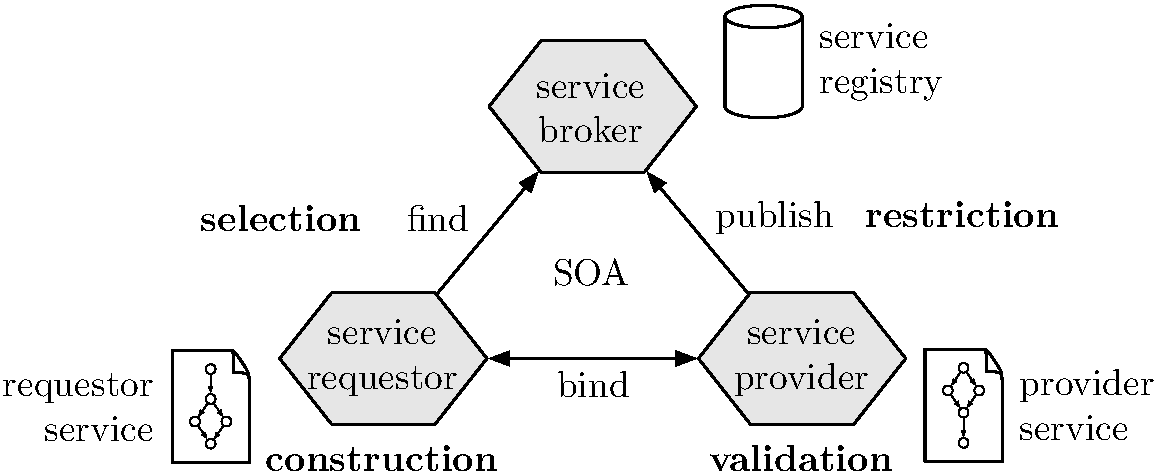
\includegraphics[scale=0.45]{validation/soa-triangle-scenarios}
\caption{Scenarios of behavioral constraints in an \acronym{SOA}.}
\label{fig:3_scenarios}
\end{figure}
%%%%%%%%%%%%%%%%%%%%%%%%%%%%%%%%%%%%%%%%%%%%%%%%%%%%%%%%%%%%%%%%%%%%%%%%%%%%%%

\Autoref{fig:3_scenarios} shows how these application scenarios of behavioral constraints  can be assigned to the roles and operations of an \acronym{SOA}.





%%%%%%%%%%%%%%%%%%%%%%%%%%%%%%%%%%%%%%%%%%%%%%%%%%%%%%%%%%%%%%%%%%%%%%%%%%%%%%%
\section{Adding constraints to service automata}
\label{sect:validation_sa}
%%%%%%%%%%%%%%%%%%%%%%%%%%%%%%%%%%%%%%%%%%%%%%%%%%%%%%%%%%%%%%%%%%%%%%%%%%%%%%%

The goal of behavioral constraints is to enforce or to exclude certain behavior in the interaction of a service with its environment while maintaining compatiblity. Hence, behavioral constraints are a refinement of compatibility and its derived concept of controllability. One requirement of compatibility is that all maximal runs of a closed composition terminate in a final state (cf.~\autoref{def:compatibility}). A behavioral constraint restricts these maximal runs by only considering a subset as terminating, whereas other maximal runs are treated as deadlocking. Thereby, a behavioral constraint also restricts the set of strategies of a service. At design time of a service, however, the set of strategies and hence the set of maximal runs of the compositions with the strategies are not known. To this end, we define behavioral constraints in terms of a given service and implicitly change the runs of a composition by explicitly changing transitions of the given service. We model behavioral constraints with \emph{constraint automata}.

%%%%%%%%%%%%%%%%%%%%%%%%%%%%%%%%%%%%%%%%%%%%%%%%%%%%%%%%%%%%%%%%%%%%%%%%%%%%%%%
\begin{definition}{Constraint automaton}
\nomenclature[C]{$C$}{a constraint automaton}%
\label{def:constraint}%
Let $A=[Q_{A},q_{0_{A}},{\shortrightarrow}_{A},\Omega_{A},\mathcal{P}_{A}]$ be a service automaton. The tuple $C=[Q,q_{0},{\shortrightarrow},\Omega]$ is a \define{constraint automaton} for $A$, iff
\begin{myenumerate}
\item $Q$ is a finite set of states,
\item $q_{0}\in Q$ is an initial state,
\item ${\shortrightarrow}\subseteq Q\times (2^{{\shortrightarrow}_{A}}\setminus\{\emptyset\}) \times Q$ is a transition relation, and
\item $\Omega\subseteq Q$ is a set of final states.
\end{myenumerate}
\end{definition}
%%%%%%%%%%%%%%%%%%%%%%%%%%%%%%%%%%%%%%%%%%%%%%%%%%%%%%%%%%%%%%%%%%%%%%%%%%%%%%%

A constraint automaton for a service automaton $A$ is a finite state automaton whose transitions are labeled with nonempty sets of transitions of $A$. Using these labels, a constraint automaton synchronizes with $A$. As for service automata, final states are used to model desired terminating states. The synchronization is defined as follows.

\enlargethispage*{\baselineskip}

%%%%%%%%%%%%%%%%%%%%%%%%%%%%%%%%%%%%%%%%%%%%%%%%%%%%%%%%%%%%%%%%%%%%%%%%%%%%%%%
\begin{definition}{Product with constraint automaton}%
\nomenclature{$\otimes$}{product with constraint(-annotated) automaton}%
\label{def:product1}%
Let $A=[Q_{A},q_{0_{A}},{\shortrightarrow}_{A},\Omega_{A},\mathcal{P}_{A}]$ be a service automaton and $C=[Q_{C},q_{0_{C}},{\shortrightarrow}_{C},\Omega_{C}]$ a constraint automaton for $A$. The \define{product} of $A$ and $C$ is the service automaton $A\otimes C=[Q,q_{0},{\shortrightarrow},\Omega,\mathcal{P}_{A}]$ consisting of
\begin{myitemize}
\item $Q:=Q_{A}\times Q_{C}$,
\item $q_{0}:=[q_{0_{A}},q_{0_{C}}]$,
\item $\Omega:=\Omega_{A}\times\Omega_{C}$, and
\item $\shortrightarrow$ containing exactly the following elements: $[q_{A},q_{C}]\xrightarrow{e}[q_{A}',q_{C}']$ iff
\begin{myenumerate}
\item $q_{A}\xrightarrow{e}_{A}q_{A}'$, \smash{$q_{C}\xrightarrow{X}_{C} q_{C}'$}, and $[q_{A},e,q_{A}']\in X$ or
\item $q_{A}\xrightarrow{e}_{A}q_{A}'$, $q_{C}=q_{C}'$, and \smash{$[q_{A},e,q_{A}']\notin \bigcup_{q_{C}''\in Q_{C}}\{X\mid q_{C}\xrightarrow{X}_{C}q_{C}''\}$}.
\end{myenumerate}
\end{myitemize}
\end{definition}
%%%%%%%%%%%%%%%%%%%%%%%%%%%%%%%%%%%%%%%%%%%%%%%%%%%%%%%%%%%%%%%%%%%%%%%%%%%%%%%

The product of a service automaton $A$ and a constraint automaton~$C$ yields a service automaton with the same interface as $A$. A state of the product is a pair of a state of $A$ and a state of $C$, and the product reaches a final state iff both $A$ and $C$ reach a final state. A state transition of~$A$ either occurs synchronized with a state transition of $C$ if the former transition is part of the label of the latter transition. In case such synchronization is not possible, $A$ changes its state without synchronization, leaving $C$ in the same state; that is, $C$ \emph{stutters}.

Our product definition is similar to \emph{stuttering synchronization} which is used, for instance, in \acronym{LTL} model checking. \citet{EsparzaH_2008_unfoldings} introduced stuttering synchronization to avoid state space explosion by only synchronizing with ``relevant'' actions of a system. \emph{Our motivation of stuttering is that the constraint automaton must not restrict the behavior of~$A$, but only restricts its set of strategies.} In particular, the product must not disable transitions of $A$. This requirement was not stated explicitly in the original paper on behavioral constraints~\cite{LohmannMW_2007_bpm}. \citet{Wolf_2008_topnoc} gave a semantical definition of this \emph{monitor property} in terms of the product of a constraint with a service automaton. In this thesis, we chose a stuttering synchronization to achieve this monitor property, because this type of synchronization changes the shape of $A$ to express a particular constraint and also allows for the efficient analysis of constrained services: \Autoref{sect:validation_implementation} is devoted to implementation details.

As a result, the product of a service automaton with a constraint automaton restricts the set of strategies.

%%%%%%%%%%%%%%%%%%%%%%%%%%%%%%%%%%%%%%%%%%%%%%%%%%%%%%%%%%%%%%%%%%%%%%%%%%%%%%%
\begin{lemma}{Product constrains the set of strategies}
Let $A$ be a service automaton and $C$ a constraint automaton for $A$.\\ Then $\Strat_{k}(A\otimes C)\subseteq\Strat_{k}(A)$.
\end{lemma}
%%%%%%%%%%%%%%%%%%%%%%%%%%%%%%%%%%%%%%%%%%%%%%%%%%%%%%%%%%%%%%%%%%%%%%%%%%%%%%%

\begin{proof}
Follows directly from \autoref{def:constraint} and \autoref{def:product1}.
\end{proof}

In a finite-state compatible composition of two services $A$ and $B$, the set of terminating runs forms a regular language. A constraint automaton~$C$ for $A$ specifies a regular language over transitions of $A$. In the composition $(A\otimes C)\oplus B$, these regular languages are synchronized, yielding a subset of terminating runs. Regular languages allow to express a variety of relevant scenarios, including:
\begin{niceitemize}
\item enforcement of events (\eg, to consider only those strategies in which a delivery notification is sent),
\item exclusion of events (\eg, to exclude those strategies in which an error message is received),
\item ordering constraints (\eg, to focus on those strategies in which an invoice is never sent \emph{before} a shipping confirmation was received), and
\item numbering constraints (\eg, to check whether there exists a strategy that can order an item by sending less than two login messages).
\end{niceitemize}
Furthermore, any combinations are possible, allowing to express complex behavioral constraints.

The presented approach is, however, not applicable to nonregular languages. For instance, a constraint requiring that a terminating run must have an equal number of $a$ and $b$ events or that $a$ and $b$ events must be properly balanced (Dyck languages) cannot be expressed with a finite-state constraint automaton. Hence, $(A\otimes C)\oplus B$ could not be expressed as finite state service automaton. Similarly, constraints that affect infinite runs (\eg, certain \acronym{LTL} formulae~\cite{MannaP_1992_ltl}) cannot be expressed.

In the remainder of this section, we describe the first two applications of behavioral constraints and how they can support the service provider to validate and restrict his service $\Prov$.




%%%%%%%%%%%%%%%%%%%%%%%%%%%%%%%%%%%%%%%%%%%%%%%%%%%%%%%%%%%%%%%%%%%%%%%%%%%%%%%
\subsection*{First application scenario: Validation}

If both services $\Req$ and $\Prov$ are given, the satisfaction of a behavioral constraint (\ie, the presence or absence of certain behavior) can be verified on the composition $\Req\oplus \Prov$ using standard model checking techniques~\cite{ClarkeGD_1999_book}. However\,---\,coming back to the scenarios described in the introduction\,---\,when a service provider wants to validate his service $\Prov$ at design time, there is no fixed requestor service $\Req$.

In the validation scenario, a service provider wants to make sure that for all strategies $\Req$ of $\Prov$ the composition $\Req \oplus\Prov$ satisfies certain constraints. An example would be that payments will always be made, or that no errors occur. We suggest to describe the constraint as a constraint automaton~$C$. Then, we can analyze the product $\Prov \otimes C$ of $\Prov$ and~$C$. The operating guideline of this product characterizes all strategies $\Req$ for $\Prov$ such that $\Req \oplus \Prov$ satisfies~$C$. The benefit of this approach is that, instead of calculating all strategies $\Req$ and checking whether $\Req \oplus \Prov$ satisfies the constraint~$C$, it is possible to characterize \emph{all} $C$-satisfying strategies $\Req$. To this end, we can use the same algorithm to calculate the operating guidelines, because the product is a regular service automaton.

Formally, the validation scenario is as follows: given the provider service $\Prov$ and a constraint automaton $C$, check if $\Strat(\Prov\otimes C)\neq\emptyset$.

\enlargethispage*{\baselineskip}


%%%%%%%%%%%%%%%%%%%%%%%%%%%%%%%%%%%%%%%%%%%%%%%%%%%%%%%%%%%%%%%%%%%%%%%%%%%%%%%
\subsection*{Second application scenario: Selection}

In the selection scenario, we assume that the service registry already contains several provider services. The requestor queries this service registry to find a provider service $\Prov$ that matches with his service $\Req$ and additionally satisfies a given constraint. Similar to the validation scenario, the service requestor is not interested in checking for each matching provider service $\Prov$ whether $\Req\oplus \Prov$ satisfies this constraint. We assume that the constraint is given as constraint automaton $C$. Now, the requestor can calculate the product $\Req\otimes C$ and use this product to query the registry for matching services. That way, the consideration of constraints refines the ``find'' operation of an \acronym{SOA}: Instead of returning \emph{any} provider service $\Prov$ such that the composition with a requester service $\Req$ is compatible, only the subset of providers $\Prov$ for which $\Req \oplus \Prov$ satisfies the constraint $C$ is returned. Formally, the selection scenario is considering the question whether $(\Req\otimes C)\in\Strat(\Prov)$.

%%%%%%%%%%%%%%%%%%%%%%%%%%%%%%%%%%%%%%%%%%%%%%%%%%%%%%%%%%%%%%%%%%%%%%%%%%%%%%
\begin{figure}[t]
\centering
\subfigure[$C_{1}$\label{validation:fig:constraint5}]{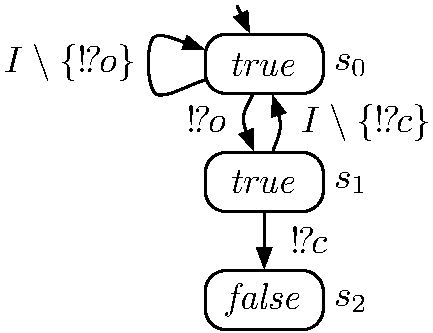
\includegraphics[scale=0.45]{validation/constraint_5}}\hspace{4em}
\subfigure[$\OG^1_{A_{\text{Buy}}\otimes C_{1}}$\label{validation:fig:product1}]{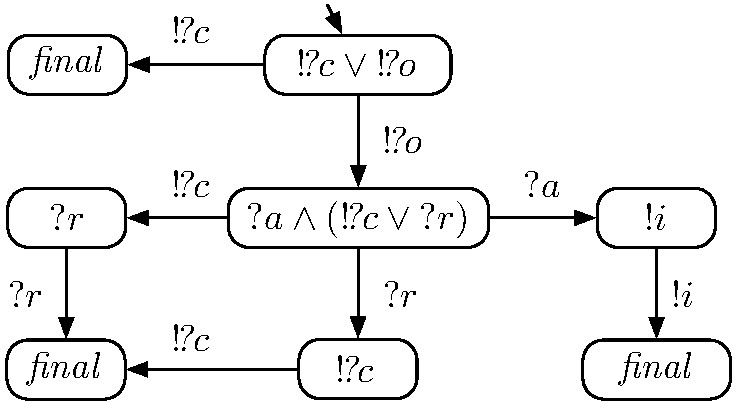
\includegraphics[scale=0.45]{validation/product_3}} 
\subfigure[$A_\text{Buy}^*\otimes C_{1}$\label{validation:fig:product2}]{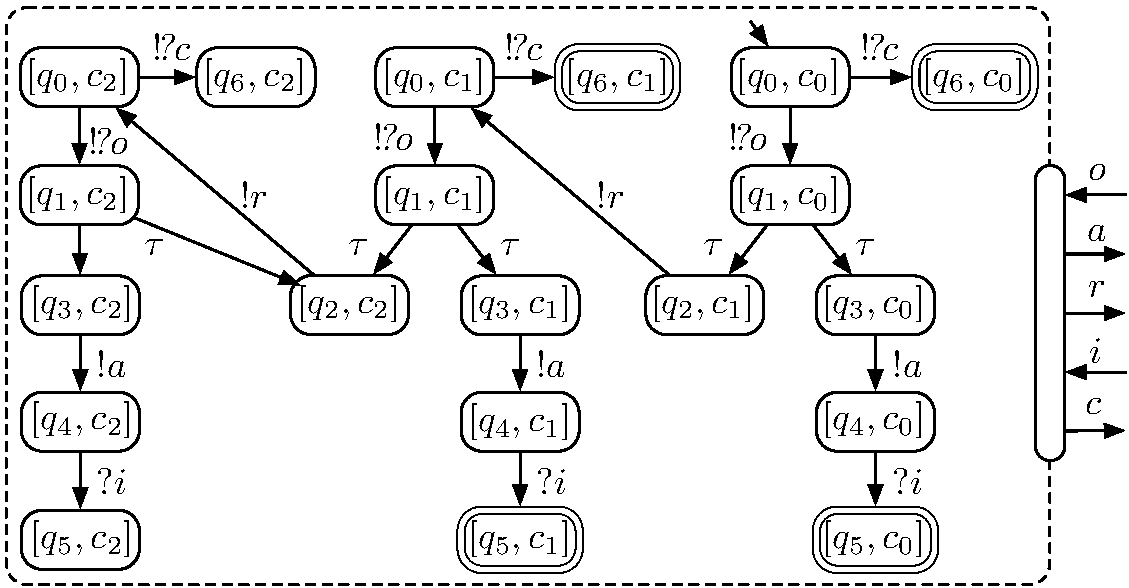
\includegraphics[scale=0.45]{validation/product_2}}
\caption{A constraint automaton expressing that at most two offers are rejected (a), the product of this constraint and the modified buyer service (c), and an operating guideline of this product~(b).}
\label{validation:fig:example1}
\end{figure}
%%%%%%%%%%%%%%%%%%%%%%%%%%%%%%%%%%%%%%%%%%%%%%%%%%%%%%%%%%%%%%%%%%%%%%%%%%%%%%

\medskip


\paragraph{Example.}

Consider again the updated buyer service in \autoref{validation:fig:buyer2}. Assume that the provider is only interested in interactions with sellers that reject at most two offers. He can formulate this requirement in a behavioral constraint. \Autoref{validation:fig:constraint5} depicts a constraint automaton, which expresses that at most two offers are rejected. \Autoref{validation:fig:product2} depicts the constrained buyer service. This product also contains two deadlocks, namely $[q_6,c_2]$ and $[q_5,c_2]$.





%%%%%%%%%%%%%%%%%%%%%%%%%%%%%%%%%%%%%%%%%%%%%%%%%%%%%%%%%%%%%%%%%%%%%%%%%%%%%%%
\section{Adding constraints to operating guidelines}\label{sect:validation_og}
%%%%%%%%%%%%%%%%%%%%%%%%%%%%%%%%%%%%%%%%%%%%%%%%%%%%%%%%%%%%%%%%%%%%%%%%%%%%%%%

The previous section was devoted to support the service provider to validate his service and the service requestor to query a service registry. The desired behavioral restriction was formulated as constraint automaton. In both scenarios, an operational description of the service (\ie, a service automaton) was available.

In case such an operational description is not accessible, constraint automata cannot be used any more. This excludes the service broker who usually has no access to an operational model, but rather stores service descriptions, such as operating guidelines. However, the service broker plays a central role in the \acronym{SOA} paradigm, comparable to a search engine in the World Wide Web. Thus, the question arises whether it is still possible to satisfy a given constraint \emph{after} having published the service $\Prov$; that is, only an operating guideline is accessible. In this section, we extend our operating guideline approach to this regard. We show that it is possible to describe a constraint as an annotated automaton~$C^\varphi$, called \emph{constraint-annotated automaton}, and apply it by building the product of $C^\varphi$ and the operating guideline $\OG_\Prov$. The resulting constrained operating guideline guideline $C^\varphi \otimes \OG_\Prov$ shall describe the set of all requester services $\Req$ such that $\Req \oplus \Prov$ satisfies the constraint.

An advantage of this setting is that we do not need the original service automaton model of $\Prov$, but can apply constraints directly to the operating guideline $\OG_\Prov$. This operating guideline contains no trade secrets and is assumed to be public to the service broker. A drawback, however, is that for the same reason we are not able to enforce, exclude, or order concrete transitions of the service automaton any more: $C^\varphi$ may only constrain send or receive actions as such. For example, if two or more transitions send a message $a$, then a constraint $C^\varphi$ excluding $a$ means that all the original transitions are excluded.

A constraint-annotated automaton for a service automaton $A$ is an annotated automaton with the same interface as $A$.

%%%%%%%%%%%%%%%%%%%%%%%%%%%%%%%%%%%%%%%%%%%%%%%%%%%%%%%%%%%%%%%%%%%%%%%%%%%%%%%
\begin{definition}{Constraint-annotated automaton}
Let $A$ be a single-port service automaton. An annotated automaton $C^\varphi$ is a \define{\mbox{constraint}-annotated automaton for $A$} iff $A$ and $C^\varphi$ have the same interface.
\end{definition}
%%%%%%%%%%%%%%%%%%%%%%%%%%%%%%%%%%%%%%%%%%%%%%%%%%%%%%%%%%%%%%%%%%%%%%%%%%%%%%%

Both the operating guideline to be constrained and the constraint-annotated automaton characterize a set of matching services with the same interface. To apply the constraint to the operating guideline, we again synchronize the automata and construct a product.

%%%%%%%%%%%%%%%%%%%%%%%%%%%%%%%%%%%%%%%%%%%%%%%%%%%%%%%%%%%%%%%%%%%%%%%%%%%%%%%
\begin{definition}{Product of annotated automata}
\label{def:product_og}%
The product of two annotated automata $A^{\varphi}$ and $B^{\psi}$ with the same interface $\mathcal{P}$ is the annotated automaton $A^{\varphi}\otimes B^{\psi}=\bigl[[Q,q_{0},{\shortrightarrow},\mathcal{P}],\zeta\bigr]$ consisting of:
\begin{myitemize}
\item $Q:=Q_{A}\times Q_{B}$,
\item $q_{0}:=[q_{0_{A}},q_{0_{B}}]$,
\item $[q_{A},q_{B}]\xrightarrow{e}[q_{A}',q_{B}']$ iff $q_{A}\xrightarrow{e}_{A} q_{A}'$ and $q_{B}\xrightarrow{e}_{B}q_{B}'$, and
\item $\zeta([q_{A},q_{B}]):=\varphi(q_{A})\wedge\psi(q_{B})$.
\end{myitemize}
\end{definition}
%%%%%%%%%%%%%%%%%%%%%%%%%%%%%%%%%%%%%%%%%%%%%%%%%%%%%%%%%%%%%%%%%%%%%%%%%%%%%%%

Structurally, the previous definition is a standard product operation of finite automata which is used to describe the intersection of regular languages~\cite{HopcroftMU_1979}. We can observe the following relation between two services and their product.

%%%%%%%%%%%%%%%%%%%%%%%%%%%%%%%%%%%%%%%%%%%%%%%%%%%%%%%%%%%%%%%%%%%%%%%%%%%%%%%
\begin{corollary}{Services simulate their product}
\label{cor:simulationproduct}%
Let $A^{\varphi}$ and $B^{\psi}$ be annotated automata and $A^{\varphi}\otimes B^{\psi}$ their product.\\ Then $A^{\varphi}$ simulates $A^{\varphi}\otimes B^{\psi}$ and $B^{\psi}$ simulates $A^{\varphi}\otimes B^{\psi}$.
\end{corollary}
%%%%%%%%%%%%%%%%%%%%%%%%%%%%%%%%%%%%%%%%%%%%%%%%%%%%%%%%%%%%%%%%%%%%%%%%%%%%%%%

%%%%%%%%%%%%%%%%%%%%%%%%%%%%%%%%%%%%%%%%%%%%%%%%%%%%%%%%%%%%%%%%%%%%%%%%%%%%%%
\begin{proof}
The existence of the simulation relations $\varrho_{(A^{\varphi}\otimes B^{\psi},A^{\varphi})}$ and $\varrho_{(A^{\varphi}\otimes B^{\psi},B^{\psi})}$ follows directly from \autoref{def:product_og}. In particular, for any reachable state $[q_{A},q_{B}]$ of $A^{\varphi}\otimes B^{\psi}$ we have $[[q_{A},q_{B}],q_{A}]\in\varrho_{(A^{\varphi}\otimes B^{\psi},A^{\varphi})}$ and $[[q_{A},q_{B}],q_{B}]\in\varrho_{(A^{\varphi}\otimes B^{\psi},B^{\psi})}$.
\end{proof}
%%%%%%%%%%%%%%%%%%%%%%%%%%%%%%%%%%%%%%%%%%%%%%%%%%%%%%%%%%%%%%%%%%%%%%%%%%%%%%

In addition, \autoref{def:product_og} also considers the annotated formulae. These formulae are conjuncted, which yields an intersection of the characterized services:

%%%%%%%%%%%%%%%%%%%%%%%%%%%%%%%%%%%%%%%%%%%%%%%%%%%%%%%%%%%%%%%%%%%%%%%%%%%%%%%
\begin{lemma}{Product yields intersection}\label{lemma:productintersection}%
Let $A^{\varphi}$ and $B^{\psi}$ be annotated automata.\\ Then $\Match(A^{\varphi}\otimes B^{\psi})=\Match(A^{\varphi})\cap\Match(B^{\psi})$.
\end{lemma}
%%%%%%%%%%%%%%%%%%%%%%%%%%%%%%%%%%%%%%%%%%%%%%%%%%%%%%%%%%%%%%%%%%%%%%%%%%%%%%%


%%%%%%%%%%%%%%%%%%%%%%%%%%%%%%%%%%%%%%%%%%%%%%%%%%%%%%%%%%%%%%%%%%%%%%%%%%%%%%%
\begin{proof} We prove the lemma by showing that $S\in\Match(A^{\varphi}\otimes B^{\psi})$ iff $S\in\Match(A^{\varphi})$ and $S\in\Match(B^{\psi})$.

\begin{labeling}{($\subseteq$)}
\item[($\Rightarrow$)]
By assumption $S\in\Match(A^{\varphi}\otimes B^{\psi})$, so there exists a structural matching relation $\varrho_{(S,A^{\varphi}\otimes B^{\psi})}$. By \autoref{cor:simulationproduct}, there exists a simulation relation $\varrho_{(A^{\varphi}\otimes B^{\psi},A^{\varphi})}$. We define the relation $\varrho_{(S,A^{\varphi})}\subseteq Q_{S}\times Q_{A^{\varphi}}$ as follows: $[q_{S},q_{A}]\in\varrho_{(S,A^{\varphi})}$ iff $[q_{S},[q_{A},q_{B}]]\in\varrho_{(S,A^{\varphi}\otimes B^{\psi})}$ and $[[q_{A},q_{B}],q_{A}]\in\varrho_{(A^{\varphi}\otimes B^{\psi},A^{\varphi})}$. The relation $\varrho_{(S,A^{\varphi})}$ is a structural matching relation between $S$ and $A^{\varphi}$.

Let $[q_{S},q_{A}]\in\varrho_{(S,A^{\varphi})}$ be arbitrary. By assumption, $q_{S}\models \varphi(q_{A})\wedge \psi(q_{B})$. Hence $q_{S}\models \varphi(q_{A})$ and $S\in\Match(A^{\varphi})$. The arguments for $S\in\Match(B^{\psi})$ are analogous.

\item[($\Leftarrow $)] Let $S\in\Match(A^{\varphi})$ and $S\in\Match(B^{\psi})$. Let $q_{S}$ be an arbitrary state of $S$, and let $q_A$ and $q_B$ be corresponding states with $[q_{S},q_{A}]\in \varrho_{({S}, A)}$ and $[q_{S},q_{B}]\in\varrho_{({S}, B)}$, respectively. Then, the state $[q_A, q_B]$ is reachable in $A^\varphi \otimes B^\psi$ and $[q_{S}, [q_A, q_B]] \in \varrho_{(S, A^\varphi \otimes B^\psi)}$. Hence, $S$ matches with $A^\varphi \otimes B^\psi$. Finally, as the assignment $\beta(q_{S})$ satisfies the annotation $\varphi(q_A)$ and the annotation $\psi(q_B)$ of matching states in $A$ or $S$, $\beta(q_{S})$ satisfies their conjunction $\varphi(q_A)\wedge \psi(q_B)$ as well.
\end{labeling}\vspace{-1em}
\end{proof}
%%%%%%%%%%%%%%%%%%%%%%%%%%%%%%%%%%%%%%%%%%%%%%%%%%%%%%%%%%%%%%%%%%%%%%%%%%%%%%%

\Autoref{lemma:productintersection} allows us to restrict the set of strategies of a provider service that do not satisfy a given constraint by calculating a product: The set $\Match(\OG_{\Prov})\cap \Match(C^{\varphi})$ is characterized by $\OG_{\Prov\otimes C^{\varphi}}$. With this result, we are able to realize the last two scenarios described in the introduction of this section. As already seen in our example, in these scenarios the constraint is modeled as a constraint-annotated automaton~$C^\varphi$. This constraint characterizes the set of accepted behaviors and can be formulated without knowing the structure of the operating guideline needed later on. Only the interface (\ie, the set of input and output message channels of the corresponding service automaton) must be known.




%%%%%%%%%%%%%%%%%%%%%%%%%%%%%%%%%%%%%%%%%%%%%%%%%%%%%%%%%%%%%%%%%%%%%%%%%%%%%%%
\subsection*{Third application scenario: Restriction}

In this scenario, the service broker wants to ensure that certain constraints are satisfied by the services in his repository. We assume that the service provider formulates his requirements as a constraint-annotated automaton $C^{\varphi}$. For each operating guideline stored in the service registry, the service broker can now calculate the product of this operating guideline and the constraint. That is, the restriction scenario can be formalized as considering $\Match(\OG_\Prov\otimes C^{\varphi})$. In case the resulting operating guidelines characterizes a nonempty set of strategies, the constraint is satisfiable. Otherwise, the operating guideline can be removed from the registry; \citet{Massuthe_2009_phd} provides an algorithm to check whether an operating guideline characterizes a nonempty set of strategies. For new provider services to be registered, the service broker has the choice to either calculate the product himself or to publish his constraint. In the latter case, the service provider applies the constraint and publishes $\OG_{\Prov \otimes C}$ in the service registry.

The service $\Prov$, however, can remain unchanged. This is an advantage as\,---\,in\-stead of adjusting, reimplementing, and maintaining several versions of $\Prov$ for each registry and constraint\,---\,only a single service $\Prov$ has to be deployed. From this service the constrained operating guidelines are constructed and published. If, for example, $\Prov$ supports credit card payment and cash on delivery, then only the strategies using credit card payments would be published to the registry mentioned before. Although there exist strategies $\Req$ for $\Prov$ using cash on delivery, those requesters would not match with the published operating guideline.




%%%%%%%%%%%%%%%%%%%%%%%%%%%%%%%%%%%%%%%%%%%%%%%%%%%%%%%%%%%%%%%%%%%%%%%%%%%%%%%
\subsection*{Fourth application scenario: Construction}

In the fourth scenario, the requester service $\Req$ is yet to be constructed. Therefore, the desired features of $\Req$ are described as a constraint-annotated automaton. For example, consider a requester who wants to book a flight paying with credit card. If these features are expressed as a constraint automaton $C^\varphi$, it can be sent to the broker who may return operating guidelines of all provider services $\Prov$ offering these features (\ie, where the product of $\OG_\Prov$ with $C^\varphi$ is not empty). From such an operational descriptions, the service $\Req$ can easily be constructed. Formally, $\Req\in\Match(\OG_\Prov\otimes C^{\varphi})$.

An important aspect of this construction scenario is that the constraint does not need to explicitly specify intermediate steps. This allows the requestor to coarsely describe his desired goals (\eg, receive a plane ticket and pay with credit card) without caring about other protocol steps (\eg, logging in or confirming the terms of payment). These intermediate steps can be specified as ``wildcards'' in the constraint.

%%%%%%%%%%%%%%%%%%%%%%%%%%%%%%%%%%%%%%%%%%%%%%%%%%%%%%%%%%%%%%%%%%%%%%%%%%%%%%
\begin{figure}
\centering
\subfigure[$C_{2}^{\varphi}$\label{validation:fig:false}]{\makebox[0.3\textwidth]{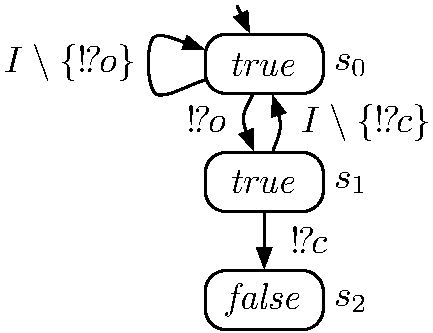
\includegraphics[scale=0.45]{validation/constraint_4}}}\hfill
\subfigure[$\OG_{A_\text{Buy}^{*}}^{1}\otimes C_{2}^{\varphi}$]{\makebox[0.6\textwidth]{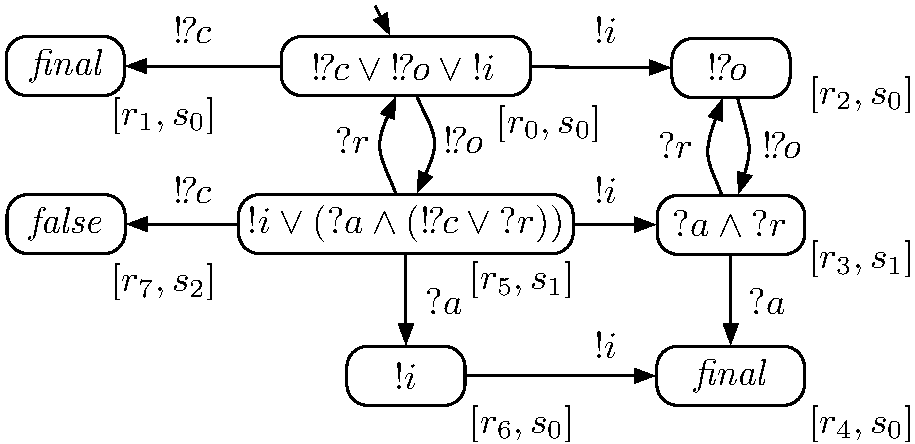
\includegraphics[scale=0.45]{validation/product_1}}}
\caption{A constraint-annotated automaton (a) expressing behavior that excludes offers that are immediately canceled and the product with the operating guideline of the buyer service (b).}
\label{validation:fig:example2}
\end{figure}
%%%%%%%%%%%%%%%%%%%%%%%%%%%%%%%%%%%%%%%%%%%%%%%%%%%%%%%%%%%%%%%%%%%%%%%%%%%%%%

\medskip


\paragraph{Example.}

In a restriction scenario, a service broker might want to exclude those services that allow to place offers and immediately cancel the negotiation afterward. \Autoref{validation:fig:example2} depicts a constraint-annotated automaton characterizing all strategies in which an order ($o$) is never directly followed by a cancellation ($c$). In the figure, edges annotated with sets are a shortcut notation for several edges, each labeled with a single element of the set. Such annotations, for instance $I\setminus \{\sync c\}$, can be seen as wildcards that match any label but $\sync c$.





%%%%%%%%%%%%%%%%%%%%%%%%%%%%%%%%%%%%%%%%%%%%%%%%%%%%%%%%%%%%%%%%%%%%%%%%%%%%%%%
\section{Implementation and experimental results}
\label{sect:validation_implementation}
%%%%%%%%%%%%%%%%%%%%%%%%%%%%%%%%%%%%%%%%%%%%%%%%%%%%%%%%%%%%%%%%%%%%%%%%%%%%%%%

The product operations on service automata and operating guidelines presented in this chapter have been prototypically implemented.

A constraint automaton usually introduces deadlocks, as for instance state $[q_{6},c_{2}]$ in \autoref{validation:fig:product2}. Consequently, a maximal terminating run in $A\oplus B$ might reach a deadlock in $(A\otimes C)\oplus B$. The tool Wendy~\cite{LohmannW_2009_wendy}, which synthesizes strategies and calculates operating guidelines, also implements \emph{early deadlock detection}. It analyzes the state space of a given open net (which coincides with a service automaton) and marks states from which a deadlock will eventually be reached. If such an ``inevitable deadlock'' is reached during the strategy synthesis, the algorithm does not generate successor states, because the current state will eventually deadlock and hence will not be part of a strategy. This dramatically prunes the state space and still synthesizes most-permissive strategies and operating guidelines. Therefore, an increased size of the product does not necessarily result in longer runtime of subsequent strategy synthesis or the calculation of the operating guidelines.



%%%%%%%%%%%%%%%%%%%%%%%%%%%%%%%%%%%%%%%%%%%%%%%%%%%%%%%%%%%%%%%%%%%%%%%%%%%%%%
\begin{table}
\centering
\caption{Experimental results for the validation scenario using Wendy.}
\medskip
\label{tab:synthesisvalidation}
\footnotesize
\begin{tabular*}{\textwidth}{@{\extracolsep{\fill}}lrrrrrr}
\toprule
& \multicolumn{3}{c}{analyzed service automaton} & \multicolumn{3}{c}{synthesis result} \\ 
constraint & \multicolumn{1}{c}{$|Q_{\otimes}|$} & \multicolumn{1}{c}{$|{\shortrightarrow}_{\otimes}|$} & \multicolumn{1}{c}{\hspace{-1em}deadlocks} & \multicolumn{1}{c}{$|Q_{\TS}|$} & \multicolumn{1}{c}{$|{\shortrightarrow}_{\TS}|$} & \multicolumn{1}{c}{\hspace{-1em}time (sec)} \\ \midrule
no constraint &     $8{,}345$ & $34{,}941$ & $0$ & $20{,}818$ & $144{,}940$ &  $29$ \\ %-m3
numbering constraint &     $26{,}667$ & $110{,}064$ & $102$ & $1{,}972$ & $11{,}686$ &  $7$ \\ %-m3
enforcement constraint &     $15{,}531$ & $66{,}625$ & $37$ & $23{,}164$ & $156{,}796$ &  $36$ \\ %-m3
exclusion constraint &     $20{,}531$ & $85{,}053$ & $125$ & $22{,}880$ & $155{,}390$ &  $36$ \\ %-m3
ordering constraint &     $9{,}110$ & $37{,}616$ & $24$ & $20{,}786$ & $144{,}796$ &  $29$ \\ %-m3
\bottomrule
\end{tabular*}
\end{table}
%%%%%%%%%%%%%%%%%%%%%%%%%%%%%%%%%%%%%%%%%%%%%%%%%%%%%%%%%%%%%%%%%%%%%%%%%%%%%%

\Autoref{tab:synthesisvalidation} lists experimental results for the validation scenario. We applied several behavioral constraints to a service automaton model (``\acronym{SMTP} protocol'' in \autoref{tab:synthesis}) translated from a \acronym{WS-BPEL} process. For the different constraints, the size of the product (columns ``$|Q_{\otimes}|$'' and ``$|{\shortrightarrow}_{\otimes}|$'') is up to three times larger than the original service. At the same time, the runtime of the synthesis of a most-permissive strategy hardly increases, because of the early detection of the deadlocks that are introduced by the product. We refer the interested reader to~\cite{LohmannW_2009_wendy}.

The calculation of the product of two annotated automata has been implemented in the tool Fiona~\cite{MassutheW_2008_awpn,Massuthe_2009_phd}. First, the product of the underlying service automata is built by performing a coordinated depth-first search. This search avoids the calculation of unreachable states. In case one annotated automaton is an operating guideline (as motivated in the third and fourth scenario), this product calculation is very efficient, because operating guidelines are deterministic by construction. During this calculation, also the product's states are annotated with the conjunction of the individual service's formulae. In a final step, each state with an unsatisfiable formulae (\eg, resulting a conjunction with \emph{false}) is deleted together with its adjacent arcs. This is repeated until a fixed point is reached. While this pruning of the constrained operating guideline does not change the characterized set of strategies, it may dramatically reduce the size of the underlying service automaton and thereby speed up subsequent matching.





%%%%%%%%%%%%%%%%%%%%%%%%%%%%%%%%%%%%%%%%%%%%%%%%%%%%%%%%%%%%%%%%%%%%%%%%%%%%%%%
\section{Discussion and related work}
\label{sect:validation_related}
%%%%%%%%%%%%%%%%%%%%%%%%%%%%%%%%%%%%%%%%%%%%%%%%%%%%%%%%%%%%%%%%%%%%%%%%%%%%%%%

In the area of model checking, it is a common technique to specify desired or undesired behavior (\eg, traces that satisfy or violate a temporal logic formulae) using automata (\eg, B\"uchi automata in case of \acronym{LTL}) and to calculate the intersection of the actual and the desired behavior using the product of this automaton and the system to check. Therefore, the presented approach to use behavioral constraints to refine the set of strategies of a service is related to several approaches in the area of computer-aided verification.


\paragraph{Supervisory control, Module checking, ATL}

In these problem in-\break stances, an open system with controllable and uncontrollable actions as well as a formula (\acronym{LTL} or \acronym{CTL}) are given. Supervisory control~\cite{Ramadge87,Ramadge89} asks whether an environment \emph{exists} which controls the controllable actions such that the system satisfies the given formula. Module checking~\cite{KupfermanV_1996_cav,KupfermanVW_2001_ic, KupfermanV_2006_book} checks whether the system satisfies the formula in \emph{all possible} environments. In this setting, deadlock-freedom is a prerequisite for the composition with the environments. That is, supervisory control quantifies the environment existentially and module checking quantifies the environment universally. Alternating-time temporal logic (\acronym{ATL})~\cite{AlurHK_2002_jacm} allows to selectively quantify the environment. This approach is closest to our approach to use an operating guideline to characterize the set of all environments (\ie, strategies) such that the composition satisfies a given constraint. Admittedly, we do not consider classical temporal logics, but only simple regular constraints. However, with operating guidelines we are able to characterize all constraint-satisfying strategies\,---\,a concept that is not yet known in the field of \acronym{ATL} or \acronym{LTL} synthesis~\cite{PnueliR_1998_popl}.


\paragraph{Model checking}

The idea to constrain the behavior of a system by composing it with an automaton is also used in the area of model checking. When a component of a distributed system is analyzed in isolation, it might reach states that are unreachable in the original (composed) system. To avoid these states, \citet{GrafS90_CAV} introduce an \emph{interface specification} to constrain the global communication behavior, which is composed to the considered component and mimics the interface behavior of the original system. \citet{Valmari00_MOVEP} adds \emph{cut states} to the interface specification, which are not allowed to be reached in the composition. These states are similar to deadlocks in a constraint automaton (cf.~state $c_{2}$ in \autoref{validation:fig:constraint5}) or states of a constraint-annotated automaton with annotation \emph{false} (cf.~\autoref{validation:fig:false}).


\paragraph{Services}

There is a lot of research being done to enforce constraints in services. The originality of behavioral constraints as presented in this chapter lies in the application of constraints to the communication between a requester and a provider service (see \autoref{fig:3_scenarios}). Furthermore, the presented model of constraints allows us to refine ``find'' operation in an \acronym{SOA}.

\citet{DavulcuKR04_WWW} describe services with a logic, allowing the enforcement of constraints by logical composition of a service specification with a constraint specification. Similarly, several protocol operators, including an intersection operator are introduced by \citet{BenatallahCT06_DKE}. Although these approaches only consider synchronous communication, they are similar to our product definition (cf. \autoref{def:product1})

An approach to describe services and desired (functional or nonfunctional) requirements by \emph{symbolic labeled transition systems} is proposed by \citet{PathakBH06_ICSOC}. An algorithm then selects services such that their composition satisfies the given requirements. However, the requirements have to be very specific; that is, the behavior of the desired service has to be specified in detail. In our presented approach, the desired behavior can be described by a constraint instead of a specific workflow. However, the discovery of a composition of several services that satisfies a required constraint is subject of future work. Other approaches presented by \citet{BerardiCGM05} and recently by \citet{GiacomoP_2009_wsfm} assume a specification of a \emph{target service} which is then realized by composing available services from a registry. Again, this approach is based on synchronous communication. Furthermore, it requires the target service to be completely specified, including all intermediate steps. In contrast, the construction approach of \autoref{sect:validation_og} does not require a complete specification, but services can also be discovered using a partial specification.


\paragraph{Operating guidelines}

Both constraint automata and constraint-annotated automata allow to specify the enforcement of desired behavior and the exclusion of undesired behavior. These constraints are implicitly universally quantified. That is, a constraint requires a certain behavior to occur in \emph{all} terminating runs or in \emph{no} terminating run. Such constraints cannot express existential quantification. For instance, a requirement that it should be \emph{possible} to receive a certain message cannot be specified. \citet{StahlW_2008_bpm} fill this gap by introducing \emph{cover constraints}. These constraints can only be expressed by \emph{extended operating guidelines}, which require a global formula in addition to the formulae that are annotated to each state.

In this thesis, we already showed how set inclusion (cf.~\autoref{def:matching}) and intersection (cf.~\autoref{lemma:productintersection}) can be expressed in terms of operating guidelines. To define a union operation or negation, \citet{KaschnerW_2009_bpm} present another extension of operating guidelines with a global formula, which allows to implement a complete set algebra on operating guidelines. While these extensions increase the complexity of the set operations, especially the possibility to join sets of strategies allows to speed up the ``find'' operation of an \acronym{SOA}.

Other reasons to discard strategies might stem from the semantics of messages and causalities between messages. These aspects go beyond the protocol level. For instance, a message modeling an acknowledgment might be sent by a participant \emph{before} actually having received a request. While such an interaction might still be compatible, it is not realizable in practice. To this end, \citet{Wolf_2008_awpn,Wolf_2008_topnoc} shows how the strategy synthesis can be adjusted to respect semantics or causalities of messages.





%%%%%%%%%%%%%%%%%%%%%%%%%%%%%%%%%%%%%%%%%%%%%%%%%%%%%%%%%%%%%%%%%%%%%%%%%%%%%%%
\section{Conclusion}
\label{sect:validation_conclusion}
%%%%%%%%%%%%%%%%%%%%%%%%%%%%%%%%%%%%%%%%%%%%%%%%%%%%%%%%%%%%%%%%%%%%%%%%%%%%%%%

In this chapter, we introduced behavioral constraints as means to restrict the set of strategies to enforce or to exclude desired and undesired behavior, respectively. Behavioral constraints can be either applied to service automata or to operating guidelines. This flexibility makes behavioral constraints a valuable tool in different scenarios of an \acronym{SOA}.

These different applications of behavioral constraints contribute to the topic of this thesis\,---\,correctness of services and their composition\,---\,as follows.
\begin{niceitemize}
\item The validation scenario allows to check a service at design time. The satisfaction of a behavioral constraint can be checked with respect to \emph{any} possible communication partner of the given service. This allows to detect unintended strategies well before implementing, deploying, and publishing the service.

\item In the selection and restriction scenarios, the focus lies on correctness by construction. The composition with any service that is returned by the service broker is not only compatible, but also satisfies a given constraint. The construction scenario further supports the design of new services by declaratively querying the service registry for desired behavior.
\end{niceitemize}

We deliberately restricted the expressiveness of the behavioral constraints to regular languages. As discussed in the previous section, covering constraints or properties of infinite runs cannot be expressed. First results show that an increased expressiveness of constraints also yields in more complex characterizations of the set of strategies of a service. To this end, we decided to make the application of behavioral constraints transparent to the concept of operating guidelines~\cite{StahlW_2008_bpm,KaschnerW_2009_bpm}. As a consequence, existing tools and algorithms remain applicable. With the aforementioned translations~\cite{LohmannMSW_2006_bpm,Lohmann_2007_wsfm} from \acronym{WS-BPEL} to service automata, behavioral constraints can be applied to industrial service description languages. First case studies showed that there are hardly any runtime penalties when considering constraints while constructing a service's operating guideline.

We consider an extension of the construction scenario as a promising direction for future work. With the presented techniques, the service registry can be queried for services that satisfy a given constraint. If the constraint models complex behavior (\eg, reserving a hotel and booking a flight), it might not be satisfied by a single service. Instead, several simpler constraints could be formulated, which return several services which need to be orchestrated to achieve the composite behavior. The automatic construction of such an orchestrator could greatly facilitate the construction of new requestor services while improving the reuse of provider services.

\chapter{Diagnosis}%
\label{chap:diagnosis}%
\chapintro{This chapter is based on results published in~\cite{Lohmann_2008_wsfm}.}


\lettrine[findent=.2em,lines=2,nindent=-0.4em]{W}{e} introduced controllability as a fundamental correctness criterion for interacting service models. In the previous chapter, we presented behavioral constraints as a means to restrict the set of strategies to refine the analysis of a service. Controllability and the satisfaction of behavioral constraints can be automatically decided. The decision algorithm (cf.~\autoref{def:synthesis}) is constructive: If a strategy for a service exists, it can be synthesized and serves as a witness for controllability. If, however, the service is uncontrollable, no strategy exists and the algorithm neither returns a service nor any diagnosis information. In this chapter, we introduce a \emph{diagnosis framework for uncontrollable services}. In the next section, we present the various reasons which may make a service uncontrollable. In~\autoref{sect:diagnosis:counterexamples} and \autoref{sect:diagnosis:reduction}, we informally sketch how counterexamples for controllability (or witnesses for uncontrollability) may be presented to service modelers. \Autoref{diagnosis:sect:blacklists} is devoted to a formalization of the problem. The diagnosis algorithm is finally defined in \autoref{diagnosis:sect:algorithm} where we also discuss its implementation. \Autoref{sect:diagnosis:conclusion} concludes the chapter.





%%%%%%%%%%%%%%%%%%%%%%%%%%%%%%%%%%%%%%%%%%%%%%%%%%%%%%%%%%%%%%%%%%%%%%%%%%%%%%%
\section{Reasons for uncontrollability}\label{sect:diagnosis:reasons}
%%%%%%%%%%%%%%%%%%%%%%%%%%%%%%%%%%%%%%%%%%%%%%%%%%%%%%%%%%%%%%%%%%%%%%%%%%%%%%%

The presence of strategies (\ie,~clients, partner services, requestors, customers, etc.) is crucial for a service. To this end, controllability is a fundamental sanity check for services, and any other (behavioral) correctness criterion (\eg, stronger notions which also require the absence of livelocks in the composition) would likely further refine the set of strategies of a service. Controllability is defined as an extension of compatibility to open services, and we shall consider the requirements for compatibility when we reason about uncontrollability. A service is uncontrollable if there does not exist a composable service such that
\begin{niceenumerate}
\item every maximal run of the composition terminates in a final state,
\item the asynchronous message channels are bounded, and
\item the composition is responsive (\ie, no port is excluded from communication on infinite runs).
\end{niceenumerate}
An uncontrollable service has no strategy. Hence, we cannot analyze a concrete composition for the reasons which led to incompatible behavior. Therefore, we need to explain the absence of strategies by considering the service itself. In particular, we have to investigate the service's share of the incompatibility of the composition with \emph{any other} service. In the remainder of this section, we give examples how errors and design flaws of a single service can result in uncontrollability. We group these issues according to the three preceding requirements.




%%%%%%%%%%%%%%%%%%%%%%%%%%%%%%%%%%%%%%%%%%%%%%%%%%%%%%%%%%%%%%%%%%%%%%%%%%%%%%%
\subsection{Deadlocking run}

The algorithm suggested by \autoref{def:synthesis} removes all nodes which contain a deadlocking state; that is, a state which is neither final nor has a successor state in the composition of the service and the strategy overapproximation. Thereby, a state $[q,\mathcal{B}]$ has two components: state~$q$ representing the internal state of the service and a multiset~$\mathcal{B}$ modeling the pending asynchronous messages. These components help classify deadlocks.


\paragraph{Internal deadlock.}

First, the state $q$ of the service may be a deadlock itself; that is, $q$ is a nonfinal state without successors. We call such a state an \emph{internal deadlock}, because this deadlock is independent of a communication event. There are different reasons why a service may contain an internal deadlock:

\begin{niceitemize}
\item \emph{Design flaw.} An obvious reason for an internal deadlock is a classical design flaw. Although languages, such as \acronym{WS-BPEL}, have syntactical requirements to avoid modeling potential deadlocks, in graph-based languages, such as \acronym{BPMN}, it is possible to introduce deadlocks, for instance because of mismatching gateways. Such design flaws affect the control flow of a service and can be detected without taking the interaction into account. Classical control flow-oriented correctness notions such as soundness~\cite{Aalst_1998_jcsc} are, however, neither sufficient nor necessary for controllability of a service. We shall discuss this in \autoref{sect:diagnosis:counterexamples}.

\Autoref{diagnosis:fig:deadlock1} shows a service automaton, which contains an internal deadlock. The service nondeterministically decides whether to send an $a$-message or a $b$-message. The environment can only observe, but not influence this decision. As the deadlock cannot be avoided, the service is uncontrollable.

\item \emph{Service choreography.} Not every internal deadlock is the result of a modeling error. Another source of internal deadlocks can be the composition of several services in a service choreography. There, it is possible that the behavior of two participants is mutually exclusive leading to an internal deadlock.

\Autoref{diagnosis:fig:deadlock2} depicts two services whose composition has the same behavior as the service automaton in \autoref{diagnosis:fig:deadlock1}. The internal deadlock occurs, because the left service waits for a $d$-message and the right service waits for an $e$-message.

%%%%%%%%%%%%%%%%%%%%%%%%%%%%%%%%%%%%%%%%%%%%%%%%%%%%%%%%%%%%%%%%%%%%%%%%%%%%%%
\begin{figure}
\centering
\hfill
\subfigure[design flaw\label{diagnosis:fig:deadlock1}]{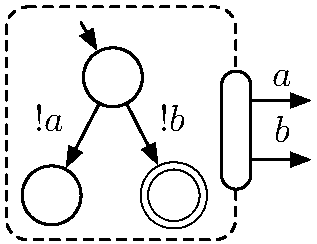
\includegraphics[scale=0.45]{diagnosis/deadlock1}} \hfill\hfill
\subfigure[deadlocking composition\label{diagnosis:fig:deadlock2}]{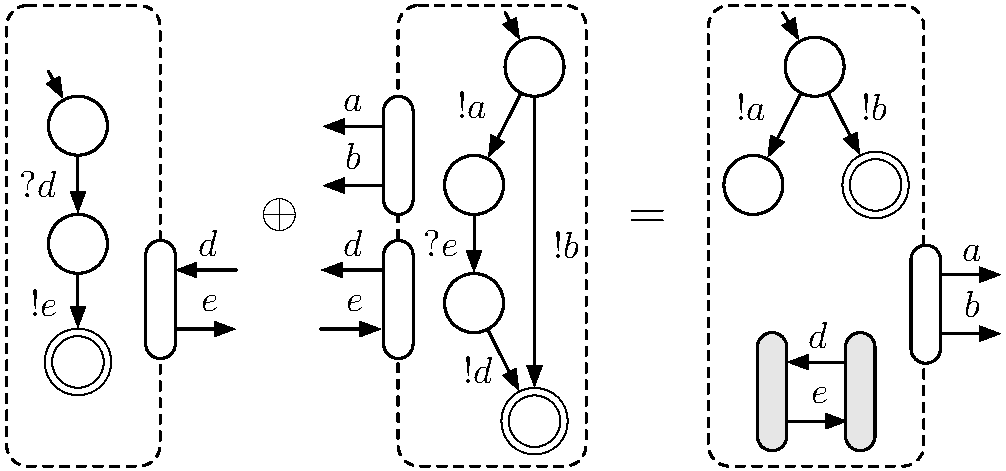
\includegraphics[scale=0.45]{diagnosis/deadlock2}}\hfill${}$
\caption{Uncontrollability caused by internal deadlocks.}
\end{figure}
%%%%%%%%%%%%%%%%%%%%%%%%%%%%%%%%%%%%%%%%%%%%%%%%%%%%%%%%%%%%%%%%%%%%%%%%%%%%%%

\item \emph{Behavioral constraint.} Another reason for internal deadlocks of a service is the consideration of a behavioral constraint $C$, cf.~\autoref{chap:validation}. In particular, final states of $A$ may become internal deadlocks in the product $A\otimes C$. These deadlocks are not design flaws, but model undesired situations. This may render a service uncontrollable as it may be impossible to satisfy the constraint.

\Autoref{validation:fig:product2} depicts a service automaton which contains the deadlocks $[q_{5},c_{2}]$ and $[q_{6},c_{2}]$ which were introduced by the constraint automaton depicted in \autoref{validation:fig:constraint5}. However, this service automaton is still controllable, because the deadlocks can be circumvented by the environment.
\end{niceitemize}


\paragraph{Covered final state.}

A \emph{covered final state} is a situation in which the control flow of $A$ reached a final state without successor state, but an asynchronous message sent to $A$ is still pending on an input channel. This message will never be received from the service. This may be negligible for generic acknowledgment messages, but an unreceived message is typically an undesired situation (\eg, if the message contains private or payment information). In addition, unexpected messages may lead to runtime errors during the execution of a \acronym{WS-BPEL} process. Again, there are many reasons for this problem:

%%%%%%%%%%%%%%%%%%%%%%%%%%%%%%%%%%%%%%%%%%%%%%%%%%%%%%%%%%%%%%%%%%%%%%%%%%%%%%
\begin{figure}
\centering
\subfigure[hidden choice\label{fig:un2}]{\makebox[0.33\textwidth]{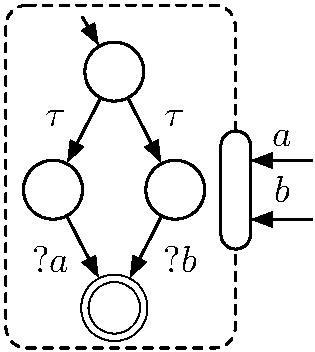
\includegraphics[scale=0.45]{diagnosis/nlc1}}}\hfill
\subfigure[conflicting receives\label{fig:un3}]{\makebox[0.33\textwidth]{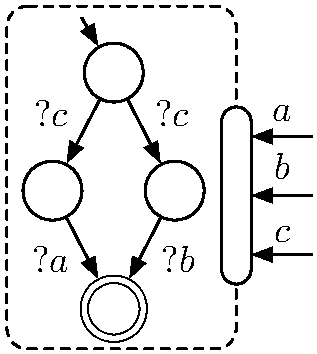
\includegraphics[scale=0.45]{diagnosis/nlc2}}}\hfill
\subfigure[delayed messages\label{fig:un4}]{\makebox[0.33\textwidth]{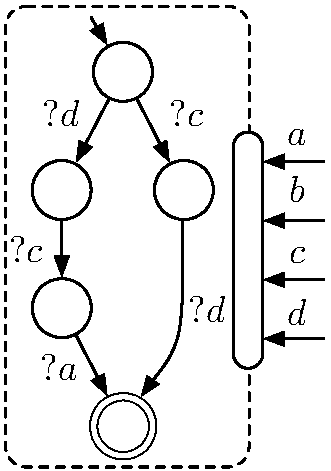
\includegraphics[scale=0.45]{diagnosis/nlc3}}}
\caption{Uncontrollability caused by covered final states.}\label{diagnosis:fig:sound}
\end{figure}
%%%%%%%%%%%%%%%%%%%%%%%%%%%%%%%%%%%%%%%%%%%%%%%%%%%%%%%%%%%%%%%%%%%%%%%%%%%%%%

\begin{niceitemize}
\item \emph{Hidden choice.} In case services implement business processes, data-dependent decisions (\eg, \acronym{WS-BPEL}'s \texttt{<if>} activity or a data-dependent gateway in \acronym{BPMN}) are common. Such a decision may be taken without explicitly informing the communication partner about the outcome. If this \emph{hidden choice} requires different reactions of the partner (\ie, the partner needs to send different messages), it cannot be guaranteed that each of these messages are received. 

Consider for example the service automaton in \autoref{fig:un2}, which nondeterministically chooses the left or the right branch. Depending on this internal choice, a partner has to send either an $a$-message or a $b$-message. The final marking is only reached, if the partner's ``guess'' was right. Otherwise, the ``wrong'' message keeps pending.

\item \emph{Conflicting receives.} If a service can reach a state in which more than one transition can receive the same message from an asynchronous channel or synchronize with the same event, these transitions are \emph{conflicting receives}~\cite{standard_bpel}. The decision which branch to take, can neither be influenced nor observed by a partner yielding a hidden choice situation. Execution languages like \acronym{WS-BPEL} treat conflicting receives as runtime faults, but similar to internal deadlocks, we do not want to forbid such situations in the first place. Instead, we want to investigate whether these problems are the original reason a service is uncontrollable.

The initial state of the service automaton in~\autoref{fig:un3} models a conflicting receive situation. After sending a $c$-message, a partner has to  send either an $a$-message or a $b$-message to the service. If the wrong choice is made, the message keeps pending on the input channel. This eventually yields a covered final state.

\item \emph{Delayed messages.} Service automata support asynchronous message exchange: messages can keep pending on a channel and overtake one other. Therefore, a partner has only limited control over a service, because after sending a message, a partner cannot observe whether this message was already received or whether it is still pending on the channel. Again, this can result in a ``hidden choice'' situation.

An example is given in \autoref{fig:un4}. The order in which the $c$-message and the $d$-message are sent to the service does not determine the order in which these messages are received and, consequently, which branch is taken. However, an $a$-message is only received if the left branch is taken and remains pending otherwise.
\end{niceitemize}

Covered final states can be seen as a ``visible symptom'' of uncontrollability rather than an original fault. For instance, there can be an arbitrary number of transitions leading from a hidden choice to covered final state. This makes the detection of the reasons which actually led to uncontrollability nontrivial.




%%%%%%%%%%%%%%%%%%%%%%%%%%%%%%%%%%%%%%%%%%%%%%%%%%%%%%%%%%%%%%%%%%%%%%%%%%%%%%%
\subsection{Exceeded message bound}

Beside the requirement that the message channels must be empty in a final state, compatibility demands that the message channels never exceed a given bound $k$. Consequently, also this message bound $k$ influences in \autoref{def:synthesis} the removal of states of $\TS^{0}(A)$ when constructing $\TS^{1}_{k}(A)$. There are two situations to consider:

%%%%%%%%%%%%%%%%%%%%%%%%%%%%%%%%%%%%%%%%%%%%%%%%%%%%%%%%%%%%%%%%%%%%%%%%%%%%%%
\begin{figure}
\centering
\subfigure[unbounded channel\label{fig:un6}]{\makebox[0.5\textwidth]{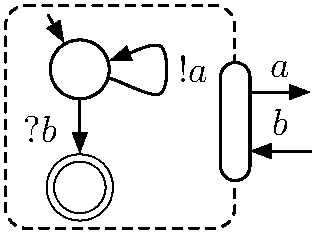
\includegraphics[scale=0.45]{diagnosis/mb1}}}\hfill
\subfigure[channel bound $k>1$\label{fig:un7}]{\makebox[0.5\textwidth]{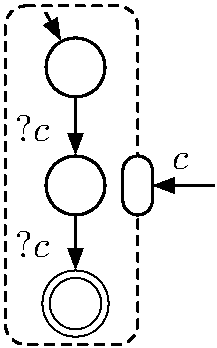
\includegraphics[scale=0.45]{diagnosis/mb2}}}
\caption{Uncontrollability caused by message bound excess ($k=1$).}
\end{figure}
%%%%%%%%%%%%%%%%%%%%%%%%%%%%%%%%%%%%%%%%%%%%%%%%%%%%%%%%%%%%%%%%%%%%%%%%%%%%%%


\paragraph{Unbounded communication.}

If a message channel is unbounded (\eg, caused by a loop of the service in which it sends messages without waiting for acknowledgements), then obviously no partner can exist such that the composition is $k$-bounded. \Autoref{fig:un6} shows an example where the output channel $a$ is unbounded. Even if the environment sends a $b$-message to this service, its receipt can be postponed arbitrarily.


\paragraph{Inadequate message bound.}

If a service is $k$-controllable for a message bound $k\in\mathds{N}^+$, it is also $l$-controllable for any bound $l>k$. The converse does not hold: \Autoref{fig:un7} shows a service which is $2$-controllable, but not $1$-controllable, because the receipt of the first $c$-message cannot be enforced before sending a second $c$-message. This results in a state where two $c$-messages are pending and the message bound is violated. Thus, even if a message bound exists for a service, this service may be considered $k$-uncontrollable if the message bound~$k$ chosen for analysis is too small. Again, we do not want to rely on the underlying infrastructure, which may enforce a message bound by discarding messages, but to treat exceeded message bounds as a design flaw we want to diagnose. Note that the message bound can be violated for output message channels (cf.~\autoref{fig:un6}) and input message channels~(cf.~\autoref{fig:un7}).




%%%%%%%%%%%%%%%%%%%%%%%%%%%%%%%%%%%%%%%%%%%%%%%%%%%%%%%%%%%%%%%%%%%%%%%%%%%%%%%
\subsection{Unresponsiveness}

\Autoref{def:synthesis} was only defined for responsive service automata. Similar to internal deadlocks, unresponsive behavior does not necessarily result in uncontrollability. Instead of restricting diagnosis to responsive services, it should be investigated whether it is the original reason of uncontrollability of a service.

%%%%%%%%%%%%%%%%%%%%%%%%%%%%%%%%%%%%%%%%%%%%%%%%%%%%%%%%%%%%%%%%%%%%%%%%%%%%%%
\begin{figure}
\centering
\subfigure[internal livelock\label{diagnosis:fig:livelock1}]{\makebox[0.5\textwidth]{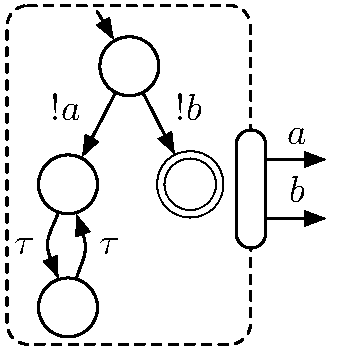
\includegraphics[scale=0.45]{diagnosis/livelock}}}\hfill
\subfigure[unresponsive communication\label{diagnosis:fig:livelock2}]{\makebox[0.5\textwidth]{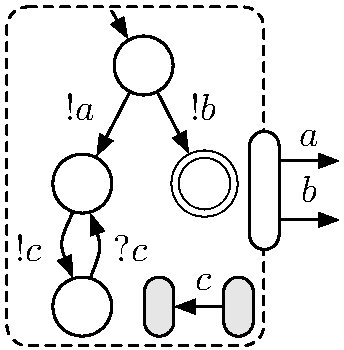
\includegraphics[scale=0.45]{diagnosis/livelock2}}}
\caption{Uncontrollability caused by unresponsive behavior.}
\end{figure}
%%%%%%%%%%%%%%%%%%%%%%%%%%%%%%%%%%%%%%%%%%%%%%%%%%%%%%%%%%%%%%%%%%%%%%%%%%%%%%


\paragraph{Internal livelock.}

A service can make a service composition unresponsive if it continuously changes its state without interaction with all ports environment and without reaching a final state. Such diverging behavior is an \emph{internal livelock} and can be checked locally similar to internal deadlocks. \Autoref{diagnosis:fig:livelock1} shows an example. An internal livelock can also model the closed communication between two implemented ports. Consider the service automaton \autoref{diagnosis:fig:livelock2}. Once this service sends an $a$-message, the port $[\emptyset,\{a,b\}]$ is excluded from further communication.

\medskip

The issues presented in this section are the original problems which can make a service uncontrollable. Deadlocks and message bound violations\,---\,\autoref{def:synthesis} only takes responsive service automata into account\,---\, yield to the deletion of such states. This deletion can introduce other deadlocks. These states usually give no further information on the original reasons which make a service uncontrollable. To this end, we focus on the detection of internal deadlocks, covered final states, and message bound violations. In addition, we have to consider unresponsive services; that is, we need to detect internal livelocks as reasons for uncontrollability.





%%%%%%%%%%%%%%%%%%%%%%%%%%%%%%%%%%%%%%%%%%%%%%%%%%%%%%%%%%%%%%%%%%%%%%%%%%%%%%%
\section{Counterexamples for controllability}
\label{sect:diagnosis:counterexamples}
%%%%%%%%%%%%%%%%%%%%%%%%%%%%%%%%%%%%%%%%%%%%%%%%%%%%%%%%%%%%%%%%%%%%%%%%%%%%%%%

As motivated the synthesis algorithm gives no information on the reasons which make a service uncontrollable. Before we elaborate on how diagnosis information could be presented, we study a related diagnosis approach.




%%%%%%%%%%%%%%%%%%%%%%%%%%%%%%%%%%%%%%%%%%%%%%%%%%%%%%%%%%%%%%%%%%%%%%%%%%%%%%
\subsection*{Relationship to soundness}

Controllability of a service model has a close relationship to soundness in the area of workflow models~\cite{Aalst_1998_jcsc}. However, existing diagnosis techniques for unsound workflow models~\cite{VerbeekBA_2001_tcj} are not applicable to diagnose uncontrollability, because the service's interaction with the environment has to be taken into account.

For a controllable service $A$ there exists service $B$ such that $A\oplus B$ are compatible. Compatibility is closely related to \emph{soundness}~\cite{Aalst_1998_jcsc}. In fact, soundness is more strict because it rules out activities which are never executed as well as livelocks. For soundness, an elaborate diagnosis algorithm exists~\cite{VerbeekBA_2001_tcj}, which exploits several properties of the soundness criterion to avoid a complex state space exploration whenever possible. For example, soundness can be expressed in terms of two simpler Petri net properties, namely \emph{liveness} and \emph{boundedness}. An unsound workflow net fails one of these tests. This result can be used to give detailed diagnosis information. In addition, several simple necessary or sufficient criteria for soundness can be checked before liveness and boundedness checks. For example, certain net classes such as \emph{free choice Petri nets}~\cite{DeselE_1995} allow for efficient analysis algorithms. However, this diagnosis approach cannot be adapted to diagnose the reasons of why a service automaton is uncontrollable.

First, a sound control flow does not imply controllability, and vice versa. For example, the control flow of the controllable service automaton in \autoref{validation:fig:product2} is not sound (due to internal deadlocks), and the uncontrollable service automata in \autoref{diagnosis:fig:sound} all have a sound control flow. Similarly, weaker criteria such as \emph{relaxed soundness} or \emph{non-controllable choice robustness}~\cite{DehnertA_2004_ijcis} are not applicable. The latter, for example, assumes that the environment can completely observe the service's state, whereas the internal state of a service can only be guessed from observations on the interface (to this end, a state of the synthesized strategy contains of a \emph{set} of states of the service together with its asynchronous interface).

Second, controllability is not a local, but a global criterion: only under restricted preconditions controllability can be decomposed~\cite{Lohmann_2008_awpn}. The previous section shows that there are multiple reasons that can make a service uncontrollable. Unfortunately, these examples cannot serve as antipatterns. Intuitively, every service that contains a bad scenario such as a hidden choice or an internal deadlock, can be extended such that the problem is either resolved or avoided in the first place (cf.~\autoref{fig:diagnosis:antipatterns}). To this end, it is impossible to consider only a fraction of the states of a service and make a statement about the correctness of the service. Therefore, only limited necessary or sufficient structural criteria for (un)controllability exist~\cite{Richter_2001_sa,Martens_2003_phd}. Finally, structural results like the invariant calculus~\cite{LautenbachR_1994_atpn} for Petri nets are not applicable, because these techniques do not take the interface into account.

%%%%%%%%%%%%%%%%%%%%%%%%%%%%%%%%%%%%%%%%%%%%%%%%%%%%%%%%%%%%%%%%%%%%%%%%%%%%%%
\begin{figure}
\centering
\subfigure[resolve problem\label{fig:diagnosis:resolve}]{\makebox[0.5\textwidth]{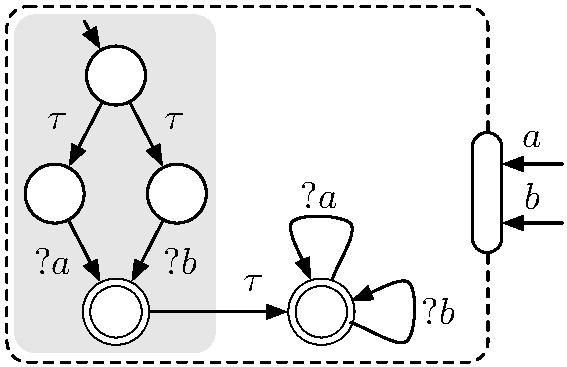
\includegraphics[scale=0.45]{diagnosis/nonlocal2}}}\hfill
\subfigure[avoid problem\label{fig:diagnosis:avoid}]{\makebox[0.5\textwidth]{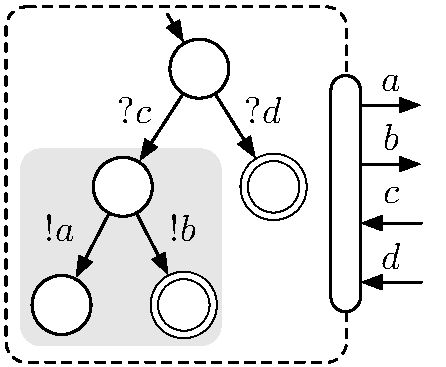
\includegraphics[scale=0.45]{diagnosis/nonlocal1}}}
\caption{Uncontrollability cannot be checked locally using antipatterns (shaded gray): pending messages can be received later~(a) and internal deadlocks can be avoided (b).}
\label{fig:diagnosis:antipatterns}
\end{figure}
%%%%%%%%%%%%%%%%%%%%%%%%%%%%%%%%%%%%%%%%%%%%%%%%%%%%%%%%%%%%%%%%%%%%%%%%%%%%%%




%%%%%%%%%%%%%%%%%%%%%%%%%%%%%%%%%%%%%%%%%%%%%%%%%%%%%%%%%%%%%%%%%%%%%%%%%%%%%%
\subsection*{Counterexamples}

In case structural methods are not applicable or can only give partial information on the correctness of a system, the \emph{behavior} of the system (\ie, its state space) needs to be analyzed. The ability to generate \emph{counterexamples} greatly boosted the acceptance of model checking~\cite{ClarkeGD_1999_book} in the field of computer-aided verification. If a model does not meet a given specification, model checking techniques automatically provide such a counterexample. For the modeler, this is a useful artifact (\eg, a deadlock trace) to understand the reasons \emph{why} the model contains an error, how it is reached, and how to fix the model. Likewise, \emph{witnesses} are useful means to prove that a system satisfies certain properties.

To find a counterexample for controllability is a nontrivial task because of the criterion's nature. Controllability is ``proved'' by constructing a witness: $A$ is $k$-controllable iff there \emph{exists} some service $B$ such that the composition $A\oplus B$ is $k$-compatible. In other words, $B$ can be seen as a counterexample for $A$'s \emph{un}controllability. If $A$ is not controllable, we can only conclude that \emph{no} such service exists, and hence cannot provide a counterexample which can be used to find out, which of the various problems we described in the previous section rendered the service uncontrollable.

The algorithm to decide controllability (cf. \autoref{def:synthesis}) overapproximates a strategy for $A$ and then iteratively removes states of this overapproximation which will not be part of any strategy of $A$. If $A$ is uncontrollable, all states will be eventually deleted. In the remainder of this section, we elaborate how a counterexample for $A$'s controllability (or a witness for $A$'s uncontrollability) should be shaped to support to locate and to understand the problems that lead to uncontrollability. In the next two sections, we then define an algorithm to use information why states are deleted from $\TS^{0}(A)$ and $\TS_{k}^{j}(A)$ to give diagnosis information for an uncontrollable service $A$.

As a motivation for the desired style of diagnosis information, consider again the service in \autoref{fig:un3}. We already described informally why this service is uncontrollable: 
\begin{quote}
After sending a $c$-message, a partner has to send either an $a$-message or a $b$-message to the service. If the wrong choice is made, the message keeps pending on the input channel. This eventually yields a covered final state.
\end{quote}

Let us analyze this informal description of why the service is uncontrollable. It contains:
\begin{labeling}{(\acronym{C})}
\item[(\acronym{I})] an indisputable initial part (``after sending a $c$-message'') which describes the communication between the service and a possible interaction partner,
\item[(\acronym{C})] a description of possible continuations (``a partner has to  send either an $a$-message or a $b$-message'') which are derived from the service's control flow, and
\item[(\acronym{P})] the problem which ultimately hinders a partner achieve compatibility of the composition (``If the wrong choice is made, the message keeps pending on the input channel. This eventually yields a covered final marking.'').
\end{labeling}

Before we explain the parts, we need to introduce \emph{waitstates}, which model situations in $\TS_0$ which can only be left with the help of the environment.

%%%%%%%%%%%%%%%%%%%%%%%%%%%%%%%%%%%%%%%%%%%%%%%%%%%%%%%%%%%%%%%%%%%%%%%%%%%%%%
\begin{definition}{Waitstate}
Let $A$ be a service automaton. The pair $[q,\mathcal{B}]\in Q_A\times\Bags(\M_a)$ is a \define{waitstate} if, for all $q\in Q_{A}$ and $e\in\E$, \smash{$q\xrightarrow{e}_A q'$} implies (1) $e\in {?\E}$ and $\mathcal{B}(\M(e))=0$ or (2) $e\in{\sync\E}$. This waitstate can be \define{resolved} by (1)~sending an asynchronous message $e$ to $A$ or by (2) synchronizing with $A$ via channel $e$, respectively.
\end{definition}
%%%%%%%%%%%%%%%%%%%%%%%%%%%%%%%%%%%%%%%%%%%%%%%%%%%%%%%%%%%%%%%%%%%%%%%%%%%%%%

A waitstate is a situation the service automaton $A$ cannot leave without communication with the environment; that is, an asynchronous message needs to be received or a synchronization with the environment is required. The notion of waitstates will be used to define the (\acronym{I}), (\acronym{C}), and (\acronym{P}) parts of the previous description. The initial part (\acronym{I}) consists of communication steps which are necessary to resolve a waitstate and which would also be taken by partners who \emph{know} the outcome of the service's decision in advance. Sending a $c$-message is not source of the problem, because this message \emph{will} be received by the service. In contrast, after sending an $a$-message, any continuation~(\acronym{C}) \emph{can} lead to a situation where reaching a final marking is not any more guaranteed. Finally, the possible problem which can occur after sending either message is described (\acronym{P}). This subtle distinction between indisputable ``safe'' interactions and problematic ``unsafe'' interactions is crucial to construct an artifact that can serve as counterexample.

In the following, we generalize this approach and elaborate the required information to define an algorithm which automatically derives such diagnosis results for an uncontrollable service $A$ consisting of these three parts:
\begin{labeling}{(\acronym{C})}
\item[(\acronym{I})] From the strategy overapproximation $\TS^{0}(A)$, we define a maximal subgraph $\TS^{0*}_{k}(A)$ such that the composition $A\oplus \TS^{0*}_{k}(A)$ is free of \emph{bad states}. A state is considered bad if it contains an internal deadlock, a covered final state, an exceeded message bound, or an internal livelock.

\item[(\acronym{C})] The subgraph $\TS^{0*}_{k}(A)$ is not a strategy of $A$, because its nodes contain waitstates which are not resolved in $\TS^{0*}_{k}(A)$, because the respective edge to a successor is missing. When these waitstates are resolved by sending messages to or by synchronizing with $A$, the composition may reach a state from which a bad state cannot be avoided any more. Therefore, in the second part of the diagnosis result, each unresolved waitstate is described including a communication trace from the initial state to the state containing this waitstate.

\item[(\acronym{P})] Finally, we give detailed information how the resolution of the waitstate can reach a bad state. For each problem, witness paths to the problematic situation or pointers to the structure of $A$ are given to locate the problem.
\end{labeling}

\Autoref{fig:diagnosis:counterexample} illustrates the overall shape of a counterexample for controllability. It is a subgraph of $\TS^{0}$ from which all blacklisted bad states~(\acronym{P}) are removed. The actual diagnosis information can then derived from those waitstates from which a transition to blacklisted states is inevitable~(\acronym{C}). The initial part~(\acronym{I}) may be empty in case a bad situation (\ie, an internal deadlock, etc.) can be reached from the initial state without interaction, cf.~\autoref{diagnosis:fig:deadlock1}. The final diagnosis algorithm will treat this case separately.

%%%%%%%%%%%%%%%%%%%%%%%%%%%%%%%%%%%%%%%%%%%%%%%%%%%%%%%%%%%%%%%%%%%%%%%%%%%%%%
\begin{figure}
\centering
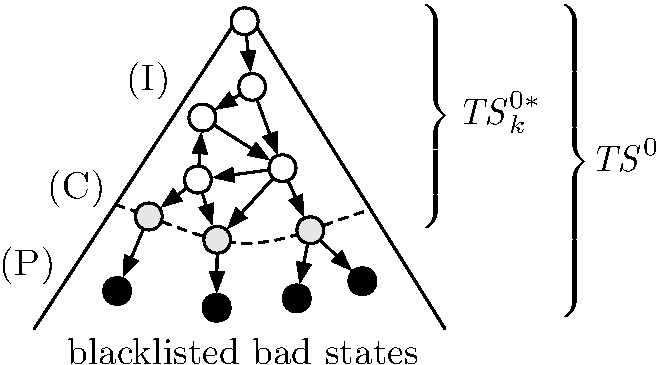
\includegraphics[scale=0.45]{diagnosis/counterexample}
\caption{A counterexample for controllability consists of an initial part (\acronym{I}), possible continuations (\acronym{C}), and resulting problems~(\acronym{P}). The subgraph $\TS^{0*}_k$ is defined using blacklists.}
\label{fig:diagnosis:counterexample}
\end{figure}
%%%%%%%%%%%%%%%%%%%%%%%%%%%%%%%%%%%%%%%%%%%%%%%%%%%%%%%%%%%%%%%%%%%%%%%%%%%%%%





%%%%%%%%%%%%%%%%%%%%%%%%%%%%%%%%%%%%%%%%%%%%%%%%%%%%%%%%%%%%%%%%%%%%%%%%%%%%%%%
\section{An overapproximation of a counterexample}
\label{sect:diagnosis:reduction}
%%%%%%%%%%%%%%%%%%%%%%%%%%%%%%%%%%%%%%%%%%%%%%%%%%%%%%%%%%%%%%%%%%%%%%%%%%%%%%%

The counterexample we sketched in the previous section is based on a subgraph of the strategy overapproximation $\TS^{0}(A)$ from \autoref{def:synthesis}. Before we go into details on how to derive this subgraph, we have to make sure that the counterexample we construct does not contain unnecessary parts.

\Autoref{def:synthesis} aims at synthesizing a most-permissive strategy for a service $A$. The algorithm achieves this by first generating the behavior of \emph{any} service communicating with $A$. This leads to several bad states in the composition $\TS^{0}(A)\oplus A$, which are iteratively removed. Only by starting out with a maximal overapproximation, most-permissiveness is guaranteed.

In case a service is uncontrollable, every state is eventually considered bad. However, not every bad state can be used to derive diagnosis information. To explain the reasons which lead to uncontrollability, the overapproximation should contain as few states as possible. In particular, messages should be only sent if they can resolve a waitstate. Likewise, receive and synchronization events should only occur if they are really possible. If we construct an overapproximation in this fashion (\ie, the construction of every state has a reason), we can derive concrete diagnosis information from bad states.

Although a smaller overapproximation is not suitable to construct a most-permissive strategy, it can dramatically speed up the synthesis of an arbitrary strategy. \citet{Weinberg_2008_wsfm} defined several on-the-fly reduction rules to find compact strategies. These strategies can be used in case only the \emph{existence} of a strategy is of interest rather than a complete characterization of all strategies satisfying the constraint.

We use two reduction rules from~\cite{Weinberg_2008_wsfm}: The first rule (called ``activated events'') avoids synthesizing unreachable behavior and only sends messages to resolve waitstates. The second rule (called ``receive before send'') prioritizes receiving events before sending events. The result is a smaller overapproximation. We adjust \autoref{def:synthesis} as follows.


%%%%%%%%%%%%%%%%%%%%%%%%%%%%%%%%%%%%%%%%%%%%%%%%%%%%%%%%%%%%%%%%%%%%%%%%%%%%%%
\begin{definition}{Reduced strategy synthesis}
\label{def:synthesisreduced}%
Let $A=[Q_{A},q_{0_{A}},{\shortrightarrow}_{A},\Omega_{A},\mathcal{P}_{A}]$ be an open finite state service automaton with $\mathcal{P}_{A}=\{[I_{1},O_{1}],\ldots,[I_{n},O_{n}]\}$. We define the open service automaton $\TS^{0}_{\textit{red}}(A)=[Q,q_{0},{\shortrightarrow},\Omega,\mathcal{P}]$ with $\mathcal{P}=\{[O,I]\mid [I,O]�\in \mathcal{P}_{A} \cap ( \M_{\mathcal{P}_{A}}^\open\times \M_{\mathcal{P}_{A}}^\open )\}$ and $Q$, $q_{0}$, ${\shortrightarrow}$, and $\Omega$ inductively as follows:
\begin{myitemize}
\item Base: Let $q_{0}:=\closure_{A}(\{[q_{0_{A}},\emptymset]\})$. Then $q_{0}\in Q$.
\item Step: For all $q\in Q$ and $m\in\M$:
\begin{enumerate}
\item If ${!m}\in \E_{\mathcal{P}}$ and $[q_{1},\mathcal{B}]\in q$ with (i) $q_{1}\xrightarrow{?m}_{A}q_{2}$, (ii) $\mathcal{B}(m)=0$, and (iii) $\mathcal{B}(m')=0$ for all $m'\in \bigcup_{j=1}^{n} I_{j}$, let $q':=\closure_{A}(\{ [q_{A},\mathcal{B}+[m]] \mid [q_{A},\mathcal{B}] \in q \})$.
Then $q'\in Q$ and \smash{$q\xrightarrow{!m}q'$}.
\item If ${?m}\in \E_{\mathcal{P}}$, let $q':=\closure_{A}(\{ [q_{A},\mathcal{B}] \mid [q_{A},\mathcal{B}+[m]] \in q \})$.\\ If $q'\neq\emptyset$, then $q'\in Q$ and $q\xrightarrow{?m}q'$.
\item If $\sync m\in \E_{\mathcal{P}}$, let $q':=\closure_{A}(\{ [q_{A}',\mathcal{B}] \mid [q_{A},\mathcal{B}] \in q$ $\wedge$ \mbox{$q_{A}\xrightarrow{\sync m}_{A}q_{A}'$}$\})$. If $q'\neq\emptyset$, then $q'\in Q$ and $q\xrightarrow{\sync m}q'$.
\end{enumerate}
\item We define $\Omega:=\{ q \in Q�\mid q \cap (\Omega_{A}\times\{\emptymset\}) \neq \emptyset \}$.
\end{myitemize}
\end{definition}
%%%%%%%%%%%%%%%%%%%%%%%%%%%%%%%%%%%%%%%%%%%%%%%%%%%%%%%%%%%%%%%%%%%%%%%%%%%%%%

From $\TS^{0}_\mathit{red}(A)$, we proceed as in \autoref{def:synthesis} by iteratively removing states where the message bound is violated or which contain deadlocks, yielding $\TS_{k_\mathit{red}}(A)$. Compared to \autoref{def:synthesis}, the following adjustments have been made:
\begin{niceitemize}
\item An asynchronous message $m$ is only sent if it resolves a waitstate and if no receiving event is possible. This is expressed by adding to (1.) the requirement that the state $q$ must contain a state $[q_{1},\mathcal{B}]$ in which (i) message $m$ can be received by $A$, (ii) that no message is pending on the input channel $m$, and that (iii) also all output channels are empty in state~$[q_{1},\mathcal{B}]$.
\item Asynchronous receive events and synchronization events are only added if they are actually possible. In \autoref{def:synthesis}, state $q'$ and transition \smash{$q\xrightarrow{?m}q'$} were added even if there exists no state $[q^{*},\mathcal{B}]\in q$ with $\mathcal{B}(m)>0$. In this case, $q'=\emptyset$ (cf.~\autoref{fig:mpp}). The same effect can occur if a synchronization event is not possible. Hence, the reduced strategy only contains states~$q$ with $q\neq\emptyset$.
\item Finally, responsiveness of $A$ is not required. If $A$ is uncontrollable, because it is unresponsive, the diagnosis algorithm should report this.
\end{niceitemize}

The first adjustment ensures that every sending event has a ``reason'', namely the resolution of a waitstate. The second adjustment rules out unreachable behavior in the overapproximation, which does not help to diagnose reasons for uncontrollability. As discussed earlier, the application of the reduction rules do not synthesize a most-permissive strategy and is therefore not applicable during the calculation of an operating guideline. However, \autoref{def:synthesisreduced} does synthesize a strategy if and only if the service is controllable~\cite{Weinberg_2008_wsfm}.

%%%%%%%%%%%%%%%%%%%%%%%%%%%%%%%%%%%%%%%%%%%%%%%%%%%%%%%%%%%%%%%%%%%%%%%%%%%%%%
\begin{proposition}{Reduced strategy proves controllability~\cite{Weinberg_2008_wsfm}}
$A$ is $k$-controllable iff \smash{$Q_{\TS_{k_\mathit{red}}(A)}\neq\emptyset$}.
\end{proposition}
%%%%%%%%%%%%%%%%%%%%%%%%%%%%%%%%%%%%%%%%%%%%%%%%%%%%%%%%%%%%%%%%%%%%%%%%%%%%%%

To put it differently: \Autoref{def:synthesisreduced} preserves the reasons for uncontrollability and $\TS^{0}_\mathit{red}(A)$ can be used as an overapproximation for a counterexample rather than $\TS^{0}(A)$.


\paragraph{Example.}

\autoref{fig:diagnosis:reduced} depicts a comparison between a most-permissive strategy and a reduced synthesized strategy. In the reduced strategy, the invoice ($i$) is only sent to resolve the waitstate $[q_{4},\emptymset]$.

%%%%%%%%%%%%%%%%%%%%%%%%%%%%%%%%%%%%%%%%%%%%%%%%%%%%%%%%%%%%%%%%%%%%%%%%%%%%%%
\begin{figure}[t]
\centering
\subfigure[$\TS_{1}(A_{Buy})$]{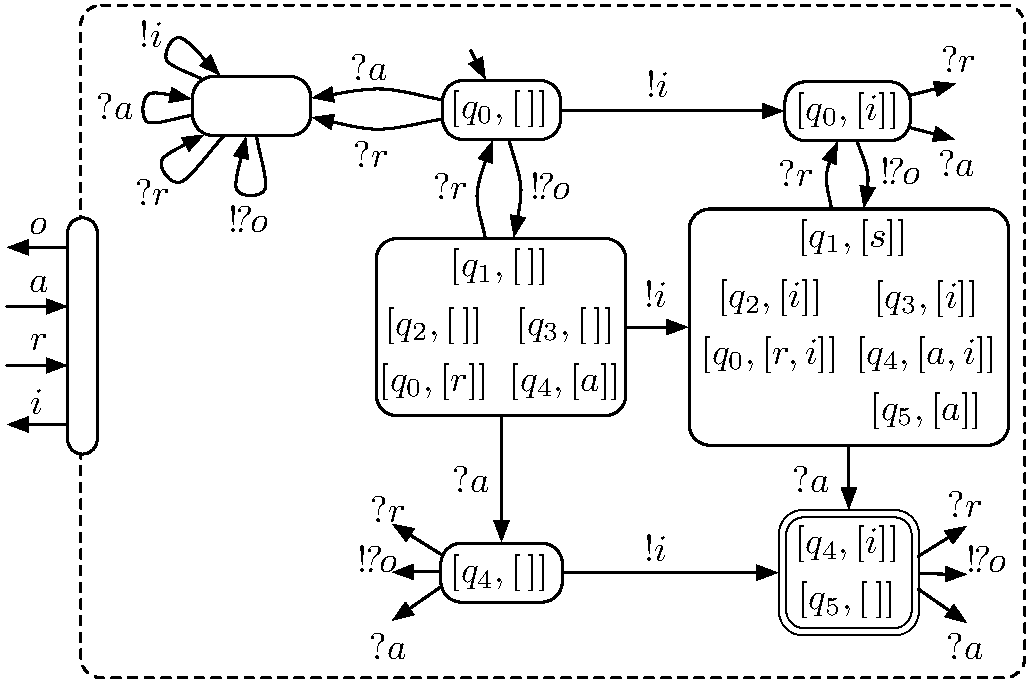
\includegraphics[scale=0.45]{background/running_mpp}}\hfill
\subfigure[$\TS_{1_\mathit{red}}(A_{Buy})$]{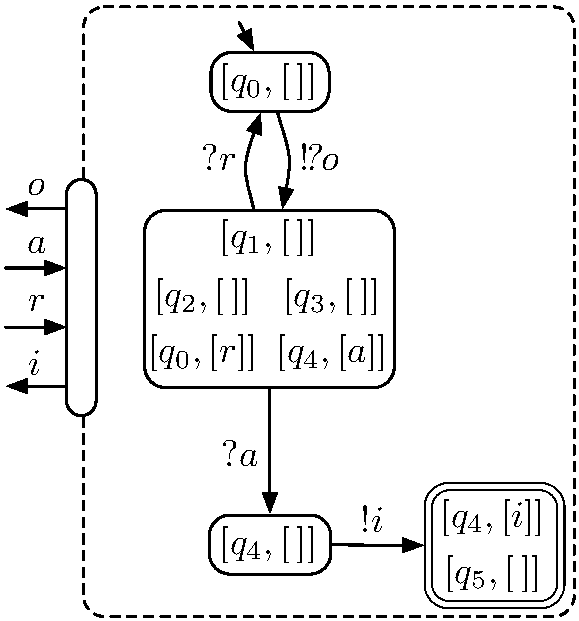
\includegraphics[scale=0.45]{diagnosis/reduced}}\caption{A most-permissive strategy (a) and the reduced synthesized strategy (b) for the buyer service from Fig.~\ref{fig:Asell}.}
\label{fig:diagnosis:reduced}
\end{figure}
%%%%%%%%%%%%%%%%%%%%%%%%%%%%%%%%%%%%%%%%%%%%%%%%%%%%%%%%%%%%%%%%%%%%%%%%%%%%%%





%%%%%%%%%%%%%%%%%%%%%%%%%%%%%%%%%%%%%%%%%%%%%%%%%%%%%%%%%%%%%%%%%%%%%%%%%%%%%%%
\section{Blacklist-based diagnosis}\label{diagnosis:sect:blacklists}
%%%%%%%%%%%%%%%%%%%%%%%%%%%%%%%%%%%%%%%%%%%%%%%%%%%%%%%%%%%%%%%%%%%%%%%%%%%%%%%

To derive diagnosis information\,---\,our counterexample demonstrating uncontrollability\,---\,, we first need a criterion to decide for each state of $\TS^{0}_\mathit{red}(A)$ whether it is a state of the subgraph $\TS^{0*}_{k}(A)$, too. We already motivated that $\TS^{0*}_{k}(A)$ should not contain bad states. Thus, for each problem, we define a \emph{blacklist} which contains such bad states. With these blacklists, we then can define the subgraph $\TS^{0*}_{k}(A)$.

For some bad states, it is also possible to characterize states which eventually \emph{will} be bad. For instance, a state whose successors are all internal deadlocks can likewise be considered bad, because once this state is reached, the service will eventually deadlock. This not only reduces the size of $\TS^{0*}_{k}(A)$, but also the length of the witness paths. Whereas the \emph{early detection} of internal deadlocks is straightforward and already exploited in the setting of behavioral constraints (cf.~\autoref{sect:validation_implementation}), the early detection of covered final states is more challenging. In particular, a covered final marking does not need to occur immediately after a hidden choice, but can occur many communication steps later.

In addition, we define a witness for each problem. A witness is an artifact which can help to locate the parts of the uncontrollable service that cause the problem (\eg, the transitions modeling a hidden choice or an internal deadlock state).




%%%%%%%%%%%%%%%%%%%%%%%%%%%%%%%%%%%%%%%%%%%%%%%%%%%%%%%%%%%%%%%%%%%%%%%%%%%%%%%
\subsection*{Blacklist for deadlocking and livelocking control flow}

Internal deadlocks and internal livelocks (\ie, unresponsive behavior) are problems that can be detected by analyzing the service in isolation. An internal livelock is a nonempty terminal strongly connected set of states of $A$, which neither contains a final state nor an open communication event. Because every internal deadlock is a (trivial) internal livelock, we can define a combined blacklist for internal deadlocks and internal livelocks as follows.

%%%%%%%%%%%%%%%%%%%%%%%%%%%%%%%%%%%%%%%%%%%%%%%%%%%%%%%%%%%%%%%%%%%%%%%%%%%%%%
\begin{definition}{Blacklist for internal deadlocks and livelocks}
We define the set of inevitable internal deadlocks of $A$, $Q_{DL}\subseteq Q_{A}$, to be the smallest set fulfilling:
\begin{myitemize}
\item If $q\not\xrightarrow{}_{A}$ and $q\notin\Omega_{A}$, then $q\in Q_{DL}$.
\item If $q\notin\Omega_{A}$ and, for all $x\in\E$, $q\xrightarrow{x}_{A} q'$ implies $q'\in Q_{DL}$, then $q\in Q_{DL}$.
\end{myitemize}

A set of states $Q_{LL}\subseteq Q_A$ is a livelock iff $Q_{LL}$ is a terminal strongly connected component of $A$ and $q\notin\Omega_{A}$ and $\lab(q)=\emptyset$, for all $q\in Q_{LL}$. Let $\mathcal{LL}$ be the set of all internal livelocks of $A$.

From these sets, define the \define{blacklist for internal deadlocks and internal livelocks} as $\bl_\mathit{DLL}:=\{q\in Q_{\TS^{0}_\mathit{red}(A)}�\mid q \cap ((Q_{DL}\cup \bigcup \mathcal{LL}) �\times \Bags(\M))�\neq \emptyset\}$. For each blacklisted state $q\in\bl_\mathit{DLL}$, define the witness $W_{DLL}(q):=\{q_d\in (Q_{DL} \cup\bigcup
\mathcal{LL})\mid [q_d,\mathcal{B}]\in q\}$.
\end{definition}
%%%%%%%%%%%%%%%%%%%%%%%%%%%%%%%%%%%%%%%%%%%%%%%%%%%%%%%%%%%%%%%%%%%%%%%%%%%%%%

We not only blacklist states which contain an internal deadlock, but also states which contain a state from which an internal deadlock will be eventually reached. For a blacklisted state $q$, the witness $W_{DLL}(q)$ is the set of all (inevitable) internal deadlocks and the internal livelocks in~$q$.




%%%%%%%%%%%%%%%%%%%%%%%%%%%%%%%%%%%%%%%%%%%%%%%%%%%%%%%%%%%%%%%%%%%%%%%%%%%%%%%
\subsection*{Blacklist for exceeded message bound}

States of the composition which exceed the message bound $k$ can be easily detected by analyzing the states occurring in nodes of $\TS^{0}_\mathit{red}$. The blacklist can be defined straightforwardly:

%%%%%%%%%%%%%%%%%%%%%%%%%%%%%%%%%%%%%%%%%%%%%%%%%%%%%%%%%%%%%%%%%%%%%%%%%%%%%%
\begin{definition}{Blacklist for exceeded message bound}
We define the \define{blacklist for exceeded message bound} as $\bl_\mathit{MB}:=\{q\in Q_{\TS^{0}_\mathit{red}(A)}\mid \exists [q^{*},\mathcal{B}]\in q : \exists m\in\M_{a}: \mathcal{B}(m)>k\}$. For each blacklisted state $q\in\bl_{MB}$, define the witness $W_{MB}(q):=\{m\in\M_a \mid \exists [q^*,\mathcal{B}]\in q : \mathcal{B}(m)>k\}$.
\end{definition}
%%%%%%%%%%%%%%%%%%%%%%%%%%%%%%%%%%%%%%%%%%%%%%%%%%%%%%%%%%%%%%%%%%%%%%%%%%%%%%

Note that the message bound may be exceeded for \emph{both} input and output channels, because the receiving of asynchronous messages may be delayed as \autoref{fig:un7} illustrates.




%%%%%%%%%%%%%%%%%%%%%%%%%%%%%%%%%%%%%%%%%%%%%%%%%%%%%%%%%%%%%%%%%%%%%%%%%%%%%%%
\subsection*{Blacklist for covered final states}

In a covered final state $q_{c}$ reachable in $A\oplus \TS^{0}_\mathit{red}(A)$, the control flow of $A$ has reached a final state which cannot be left, but a message is pending on an input channel, which cannot be received from $A$. By construction of $\TS^{0}_\mathit{red}(A)$, this message was originally sent to $A$ to resolve a waitstate (cf.~\autoref{def:synthesisreduced}). The following observation is needed to justify the later definition of a blacklist for covered final states.

%%%%%%%%%%%%%%%%%%%%%%%%%%%%%%%%%%%%%%%%%%%%%%%%%%%%%%%%%%%%%%%%%%%%%%%%%%%%%%
\begin{lemma}{Covered final states also exist uncovered}
Let $A$ be service automaton with the interface $\mathcal{P}_{A}=\{[I_{1},O_{1}],\ldots,[I_{n},O_{n}]\}$ and $\TS^{0}_\mathit{red}(A)$ as defined in \autoref{def:synthesisreduced}. Let~$q_{1}$ be a state of $\TS^{0}_\mathit{red}(A)$ and $[q_{f},\mathcal{B}+[x]]\in q_{1}$ a covered final state with $q_{f}\in\Omega_{A}$ and $x\in \bigcup_{j=1}^{n}I_{j}$.\\ Then exists a state $q_{2}$ of $\TS^{0}_\mathit{red}(A)$ with $[q_{f},\mathcal{B}]\in q_{2}$.\label{lem:covered}
\end{lemma}
%%%%%%%%%%%%%%%%%%%%%%%%%%%%%%%%%%%%%%%%%%%%%%%%%%%%%%%%%%%%%%%%%%%%%%%%%%%%%%

\Autoref{lem:covered} states that, for each covered final state with a pending $x$-message occurring in a state of $\TS^{0}_\mathit{red}(A)$, there exists a state which contains a covered final state (or a final state if $\mathcal{B}=\emptymset$) \emph{without} that pending $x$-message. \Autoref{fig:covered1} illustrates the lemma and visualizes the interrelations of the states mentions in the following proof.

%%%%%%%%%%%%%%%%%%%%%%%%%%%%%%%%%%%%%%%%%%%%%%%%%%%%%%%%%%%%%%%%%%%%%%%%%%%%%%
\begin{proof}
Let $q_{1}$ be as above. Then there exist states $q$ and $q_{x}$ of $\TS^{0}_\mathit{red}(A)$ with \smash{$q\xrightarrow{!x} q_{x}$}, and there exists a path $\sigma$  from $q_{x}$ to $q_{1}$ which does not contain an $!x$-labeled edge. Let $[q_{f},\mathcal{B}+[x]]\in q_{1}$ be as above. The pending $x$-message was only sent to $A$ to resolve a waitstate (cf.~\autoref{def:synthesisreduced}). Let $[q_{w},\mathcal{B}_{w}]\in q$ be such a waitstate.

Let $[q_{e},\mathcal{B}_{e}]\in q$ be a state of $q$. From \smash{$q\xrightarrow{!x} q_x$} we can conclude that there exists a state $[q_{e},\mathcal{B}_{e}+[x]]\in q_{x}$. Let the path $\sigma^*$ be an extension of the path $\sigma$ such that \smash{$[[q_{e},\mathcal{B}_{e}+[x]],q_{x}]\xrightarrow{\sigma^*} [[q_{f},\mathcal{B}+[x]], q_{1}]$} in the composition \smash{$A\oplus \TS^{0}_\mathit{red}(A)$.} This path~$\sigma^*$ does not contain a transition labeled with $!x$, because \smash{$\sigma^*|_{\TS^{0}_\mathit{red}(A)}=\sigma$} does not contain an $!x$-labeled transition. Therefore, $\sigma^*$ is realizable independently of (\ie, without) the pending $x$-message. In particular, there exists a state $q_{2}$ of $\TS^{0}_\mathit{red}(A)$ such that \smash{$[[q_{e},\mathcal{B}_{e}],q]\xrightarrow{\sigma^*} [[q_{f},\mathcal{B}]],q_{2}]$}.
\end{proof}
%%%%%%%%%%%%%%%%%%%%%%%%%%%%%%%%%%%%%%%%%%%%%%%%%%%%%%%%%%%%%%%%%%%%%%%%%%%%%%

After iteratively applying \autoref{lem:covered}, we can conclude that with each covered final state occurring in $\TS^{0}_\mathit{red}(A)$, also a respective ``uncovered'' final marking is present in a state of $\TS^{0}_\mathit{red}(A)$.

%%%%%%%%%%%%%%%%%%%%%%%%%%%%%%%%%%%%%%%%%%%%%%%%%%%%%%%%%%%%%%%%%%%%%%%%%%%%%%
\begin{figure}
\centering
\subfigure[illustration for \autoref{lem:covered}\label{fig:covered1}]{\makebox[0.49\textwidth]{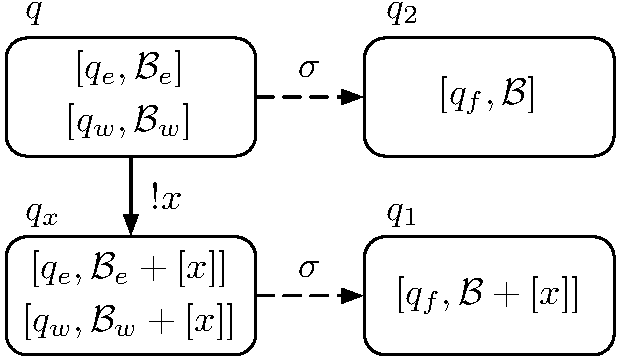
\includegraphics[scale=0.45]{diagnosis/covered}}}
\subfigure[hidden choice transition of \autoref{def:cfm}\label{fig:covered2}]{\makebox[0.49\textwidth]{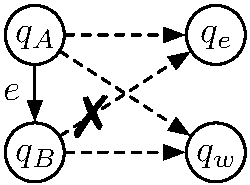
\includegraphics[scale=0.45]{diagnosis/covered2}}}
\caption{Illustrations for \autoref{lem:covered} and \autoref{def:cfm}.}
\label{fig:covered}
\end{figure}
%%%%%%%%%%%%%%%%%%%%%%%%%%%%%%%%%%%%%%%%%%%%%%%%%%%%%%%%%%%%%%%%%%%%%%%%%%%%%%

Each application of \autoref{lem:covered} identifies an $!x$-labeled transition from~$q$ to state $q_{x}$ from which a state $q_{1}$ is reached which contains a covered final state with a pending $x$-message, which is never received. For state~$q$, an alternative continuation to $q_{2}$ without an $!x$-transition is possible.

Hence, such a state $q_{x}$ should be considered critical, which yields the following definition of a blacklist for covered final states.




%%%%%%%%%%%%%%%%%%%%%%%%%%%%%%%%%%%%%%%%%%%%%%%%%%%%%%%%%%%%%%%%%%%%%%%%%%%%%%
\begin{definition}{Blacklist for covered final states}\label{def:cfm}%
Let, $q$, $q_x$, $q_1$, $q_2$, $q_e$, and $q_w$ as defined to be as in \autoref{lem:covered} and its proof (cf.~\autoref{fig:covered1}). We define the \define{blacklist for covered final states}, $\bl_{CFS}$, to contain exactly those states~$q_x$. Define the witness for a blacklisted state $q_x$, $W_{CFS}(q_x):=\{ q_A\xrightarrow{e}_{A} q_B \mid q_A\xrightarrow{*}q_w \wedge q_B\xrightarrow{*}q_w \wedge q_A\xrightarrow{*}q_e \wedge q_B\not\xrightarrow{*}q_e \}$, to contain all \define{hidden choice transitions} of $A$.
\end{definition}
%%%%%%%%%%%%%%%%%%%%%%%%%%%%%%%%%%%%%%%%%%%%%%%%%%%%%%%%%%%%%%%%%%%%%%%%%%%%%%

A covered final state is a situation which occurs in case a service automaton $A$ is composed to a partner. With the help of \autoref{lem:covered}, the blacklist for covered final states can be defined only by checking the states of $\TS^{0}_\mathit{red}(A)$ and paths in $\TS^{0}_\mathit{red}(A)$ and $A$. This can be realized during the construction $\TS^{0}_\mathit{red}(A)$ instead of analyzing paths in $A\oplus\TS^{0}_\mathit{red}(A)$. \Autoref{lem:covered} also allows for finding a set of \emph{hidden choice transitions} (see \autoref{fig:covered2}), which model a hidden decision as described in \autoref{sect:diagnosis:reasons}. These transitions can be the starting point to repair the service to avoid the covered final state.





%%%%%%%%%%%%%%%%%%%%%%%%%%%%%%%%%%%%%%%%%%%%%%%%%%%%%%%%%%%%%%%%%%%%%%%%%%%%%%%
\section{Diagnosis algorithm}\label{diagnosis:sect:algorithm}
%%%%%%%%%%%%%%%%%%%%%%%%%%%%%%%%%%%%%%%%%%%%%%%%%%%%%%%%%%%%%%%%%%%%%%%%%%%%%%%

With the definitions of the blacklists, we are finally able to define the subgraph $\TS^{0*}_k(A)$ (i.\,e., the counterexample for controllability of $A$) of $\TS_{k_\mathit{red}}(A)$ which only contains states which are not contained in any of the blacklists. Thereby, we ignore states which have become unreachable from the initial state.

%%%%%%%%%%%%%%%%%%%%%%%%%%%%%%%%%%%%%%%%%%%%%%%%%%%%%%%%%%%%%%%%%%%%%%%%%%%%%%
\begin{algorithm}[t!]
\restylealgo{boxed}
\SetVline
\caption{Blacklist-based diagnosis for uncontrollable services}
\label{alg:diagnosis}\footnotesize
\BlankLine
\KwIn{uncontrollable finite state service automaton $A$, message bound $k$}
\KwOut{diagnosis information, $\TS^{0*}_k(A)$}
\BlankLine
{calculate $\TS^{0}_\mathit{red}(A)$}

{derive $\bl_\mathit{DLL}$} from $\TS^{0}_\mathit{red}(A)$

{derive $\bl_\mathit{EMB}$} from $\TS^{0}_\mathit{red}(A)$

{derive $\bl_\mathit{CFS}$} from $\TS^{0}_\mathit{red}(A)$
\BlankLine
\eIf{$q_{0}$ is blacklisted}{
\If{$q_{0}\in\bl_\mathit{DLL}$}{
\ForEach{witness $q^*\in W_{DLL}(q_0)$}{
{\textbf{print} ``internal deadlock/livelock $q^*$ reachable without interaction''}
}
}
\If{$q_{0}\in\bl_\mathit{EMB}$}{
\ForEach{witness $m^*\in W_{EMB}(q_0)$}{
{\textbf{print} ``message bound of channel $m^*$ exceeded without interaction''}
}
}} {
\ForEach{nonblacklisted state $q$ reachable from $q_{0}$}{
\ForEach{waitstate $[q',\mathcal{B}]\in q$ with \smash{$q'\xrightarrow{e}_A q''$} and $q_e$ with \smash{$q\xrightarrow{e} q_e$}}{
\If{$q_e$ is blacklisted}{
\textbf{print} ``resolving waitstate $[q',\mathcal{B}]$ may reach a bad state''

\If{$q_{e}\in\bl_\mathit{DLL}$}{
\ForEach{witness $q^*\in W_{DLL}(q_e)$}{
\textbf{print} ``in $q_e$: internal deadlock/livelock $q^*$ reachable''
}
}
\If{$q_{e}\in\bl_\mathit{EMB}$}{
\ForEach{witness $m^*\in W_{EMB}(q_e)$}{
\textbf{print} ``in $q_e$: message bound of channel $m^*$ violated''
}
}
\If{$q_{e}\in\bl_\mathit{CFS}$}{
\textbf{print} ``in $q_e$: message $e$ may be left unreceived''

\ForEach{witness $[q_1,x,q_2]\in W_{CFS}(q_e)$}{
\textbf{print} ``hidden choice transition: $[q_1,x,q_2]$``
}
}
}
}
}
\textbf{print} subgraph $\TS^{0*}_k$ of $\TS_\mathit{red}^0(A)$ without blacklisted states
}
\end{algorithm}
%%%%%%%%%%%%%%%%%%%%%%%%%%%%%%%%%%%%%%%%%%%%%%%%%%%%%%%%%%%%%%%%%%%%%%%%%%%%%%

Algorithm~\ref{alg:diagnosis} combines the defined blacklists together with their witnesses and gives information for each detected problem. After a preprocessing phase (line 1--4) in which $\TS^{0}_\mathit{red}$ as well as the blacklists are calculated, the states of $\TS^{0}_\mathit{red}$ are analyzed. Thereby, two cases are differentiated: If already the initial state of $q_{0}$ is blacklisted, then the service can reach a bad state independently of a partner. Covered final states cannot occur in this setting. As a diagnosis information, the initial state $q_{0}$ and the respective problems are printed (line 5--11). The remainder of the algorithm (line~12--27) treats situations in which $\TS^{0*}_k$ is nonempty.

The diagnosis messages can be classified into the three categories (initial part~\acronym({I}), possible continuation~(\acronym{C}), and occurring problem~(\acronym{P})) as follows:
\begin{labeling}{(\acronym{C})}
\item[(\acronym{I})] line 27 prints the nonblacklisted subgraph $\TS^{0*}_k$,
\item[(\acronym{C})] line 16 prints a nonblacklisted waitstate whose resolution may reach a bad state,
\item[(\acronym{P})] line 8, 11, 19, 22, 24, and 26 print information about the problem which may be unavoidable after resolving the respective waitstate, including witnesses.
\end{labeling}

\enlargethispage*{\baselineskip}

The algorithm lists all problems which can occur if $\TS^{0*}_k$ is ``left'' by resolving a waitstate. If, for example, sending an $x$-message can result in a message bound violation \emph{and} yield an internal deadlock, then both problems are reported.




%%%%%%%%%%%%%%%%%%%%%%%%%%%%%%%%%%%%%%%%%%%%%%%%%%%%%%%%%%%%%%%%%%%%%%%%%%%%%%%
\subsection*{Implementation and experimental results}

The diagnosis has been implemented into the tool Wendy~\cite{LohmannW_2009_wendy}. In a special diagnosis mode, it constructs the reduced strategy from which the blacklists are generated.

The practical applicability of the diagnosis information is hard to measure and needs further investigation. To give an impression on the runtime and the sizes of the counterexamples, \autoref{tab:redsynthesis} lists results on synthesizing reduced strategies for the services we described in~\autoref{sect:background:experiment}. The reduced strategies consist only of a fraction of states and all can be calculated in less than a second. The nonblacklisted subgraph which is used as counterexample for controllability is a subgraph of the reduced synthesized strategy, so the numbers of \autoref{tab:redsynthesis} can be seen as an upper bound for the size of the counterexample.

%%%%%%%%%%%%%%%%%%%%%%%%%%%%%%%%%%%%%%%%%%%%%%%%%%%%%%%%%%%%%%%%%%%%%%%%%%%%%%
\begin{table}[tb]
\centering
\caption{Experimental results for reduced strategy synthesis using Wendy.}\medskip
\label{tab:redsynthesis}
\footnotesize
\begin{tabular*}{\textwidth}{@{\extracolsep{\fill}}lrrrrrr}
\toprule
& \multicolumn{3}{c}{most-permissive strategy} & \multicolumn{3}{c}{reduced strategy} \\ 
service & \multicolumn{1}{c}{$|Q_{\TS}|$} & \multicolumn{1}{c}{$|{\shortrightarrow}_{\TS}|$} & \multicolumn{1}{c}{time (sec)} & \multicolumn{1}{c}{$|Q_{\TS_\mathit{red}}|$} & \multicolumn{1}{c}{$|{\shortrightarrow}_{\TS_\mathit{red}}|$} & \multicolumn{1}{c}{time (sec)} \\ \midrule
Quotation &             $11{,}264$ & $145{,}811$ &   $3$ & $62$ & $77$ & $0$ \\
Deliver goods &          $1{,}376$ &  $13{,}838$ &   $2$ & $53$ & $82$ & $0$ \\ %daniela
{\scriptsize SMTP} protocol  & $20{,}818$ & $144{,}940$ &  $29$ & $62$  & $78$ & $0$ \\ %-m3
Car analysis &    $1{,}448$ &  $13{,}863$ &  $52$ & $108$ & $183$ & $1$ \\ %daniela
Identity card &      $1{,}536$ &  $15{,}115$ & $83$ & $259$ & $1{,}027$ & $1$ \\
Product order &    $57{,}996$ & $691{,}414$ & $303$ & $461$ & $938$ & $0$ \\ %-m2
\bottomrule
\end{tabular*}
\end{table}
%%%%%%%%%%%%%%%%%%%%%%%%%%%%%%%%%%%%%%%%%%%%%%%%%%%%%%%%%%%%%%%%%%%%%%%%%%%%%%


\Autoref{fig:diagnosis:example} depicts an uncontrollable service automaton and the diagnosis output of the tool Wendy. It consists of a graphical representation of the subgraph as well as a textual description of the problems and recommendations how to fix these issues. For instance, if the violation of a given message bound is the only detected problem, then the user is advised to restart the analysis with an increased message bound. The visualization of the counterexample generated by the diagnosis algorithm is in a very early state and needs to be tightly integrated to a service modeling tool. This integration is subject to future work and out of scope of this thesis.

%%%%%%%%%%%%%%%%%%%%%%%%%%%%%%%%%%%%%%%%%%%%%%%%%%%%%%%%%%%%%%%%%%%%%%%%%%%%%%
\begin{figure}[tb]
\centering
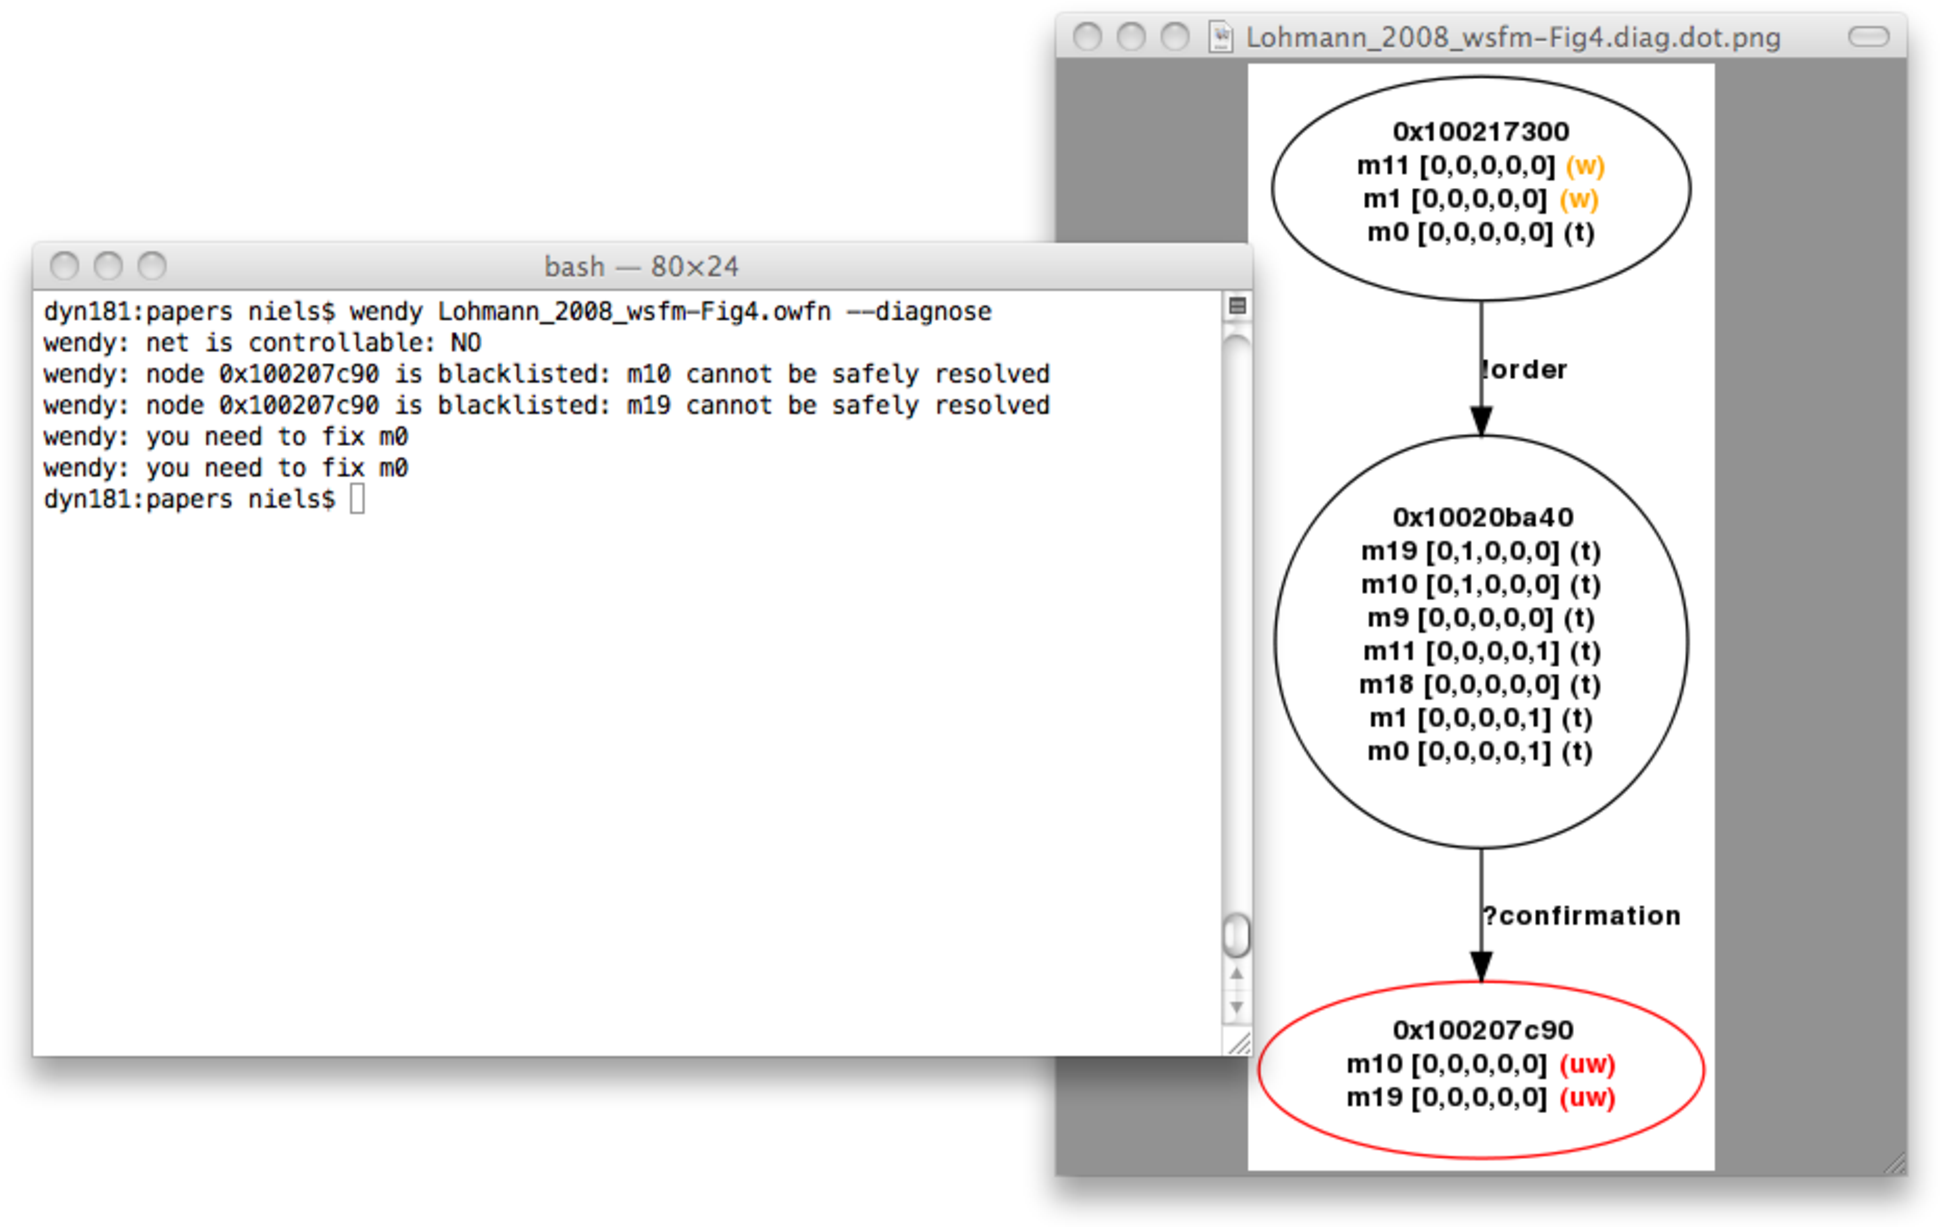
\includegraphics[width=0.8\textwidth]{diagnosis/wendydiag}
\caption{Diagnosis output of the tool Wendy.}
\label{fig:diagnosis:example}
\end{figure}
%%%%%%%%%%%%%%%%%%%%%%%%%%%%%%%%%%%%%%%%%%%%%%%%%%%%%%%%%%%%%%%%%%%%%%%%%%%%%%





%\enlargethispage*{\baselineskip}

%%%%%%%%%%%%%%%%%%%%%%%%%%%%%%%%%%%%%%%%%%%%%%%%%%%%%%%%%%%%%%%%%%%%%%%%%%%%%%%
\section{Conclusion}\label{sect:diagnosis:conclusion}
%%%%%%%%%%%%%%%%%%%%%%%%%%%%%%%%%%%%%%%%%%%%%%%%%%%%%%%%%%%%%%%%%%%%%%%%%%%%%%%

The generation of counterexamples greatly boosted the acceptance of model checking~\cite{ClarkeGD_1999_book} in the field of computer-aided verification. They present the reasons which make a model incorrect and therefore are as important as the verification procedure itself. However, the decision algorithm for controllability (cf.~\autoref{def:synthesis}) does not provide such counterexamples. In this chapter, we investigated uncontrollable service models and presented a variety of reasons why a service does not have any partners which interact in a compatible manner. We elaborated how a counterexample for controllability should be shaped to help the modeler understand the reasons which make a service uncontrollable. An algorithm to construct such a counterexample has been defined in terms of blacklists and has been prototypically implemented. The returned diagnosis information can be the starting point for corrections of the service toward controllability. We shall come back to this in \autoref{chap:correction}. The diagnosis algorithm can be directly used for refinements of controllability, for instance behavioral constraints (cf.~\autoref{chap:validation}), and is likely to be applicable to further extensions.

\medskip

Several aspects of diagnosing uncontrollable services remain subject of future work. First, service models usually stem from industrial specification languages, such as \acronym{WS-BPEL}. Hence, the retranslation of (automaton-related) diagnosis information back into \acronym{WS-BPEL} is a prerequisite to correlate the problems to the original model. Existing translations between service automata and \acronym{WS-BPEL}~\cite{Lohmann_2007_wsfm,LohmannK_2008_mod} could be extended to translate the necessary diagnosis information. In particular, a mapping between diagnosed bad states and activities in the original process could be challenging.

Second, the acceptance of the counterexamples needs to be further investigated. First experiments showed that especially hidden choices are often overlooked even by experienced service modelers. Nonlocality, asynchronous message exchange, and the absence of a concrete interaction partner are only a few of the reasons which make uncontrollable services hard to detect during modeling time.

Finally, further reduction techniques from \citet{Weinberg_2008_wsfm} may help to define a more compact counterexample for controllability. Reducing the size of the counterexample not only increases the understandability, but allows for faster calculation. This is crucial to be able to integrate the diagnosis algorithm into modeling tools. A constant analysis of a service model (\eg, each time the model is stored) helps to quickly correlate diagnosed problems to recent changes. For the soundness criterion, it is already possible to integrate verification techniques into industrial modeling tools~\cite{FahlandWJKLVW_2009_bpm} and verify the model constantly.


\part{Correctness of \mbox{Service Compositions}}\label{part2}
\chapter{Verification and Completion}\label{chap:verification}
\chapintro{This chapter is based on results published in~\cite{LohmannKLR_2007_wsfm}.}
%%%%%%%%%%%%%%%%%%%%%%%%%%%%%%%%%%%%%%%%%%%%%%%%%%%%%%%%%%%%%%%%%%%%%%%%%%%%%


\lettrine[findent=.2em,lines=2,nindent=0pt]{I}{n} the previous two chapters, we investigated the correctness of services in isolation; that is, services embedded in arbitrary environments. With the notion of controllability and behavioral constraints, we could reason about the correctness of \emph{one} service with respect to \emph{any} possible service composition. In this chapter, we go one step further and study the correctness of a \emph{concrete} composition of \emph{several} services.

As in the previous chapters, we focus on the behavior of service compositions and employ compatibility as correctness criterion. For this reason, we do not consider other aspects of composing services, such as wiring (\ie, addressing and syntactical issues), instance lifecycles (\ie, how new instances are created, who triggers instantiations, and how many ``copies'' of each service are needed), or nonfunctional properties (\eg, an agreement on encryption, policies, or quality of service). 

In the literature~\cite{Peltz_2003_ieee,DijkmanD_2004_ijcis}, two viewpoints on a service composition are distinguished: \emph{service orchestrations} and \emph{service choreographies}. They are typically considered to be complementary paradigms, whereas other authors (\eg,~\cite{PapazoglouTDL_2007_ieee}) criticize a too strict distinction. We shall come back to this discussion in \autoref{chap:realizability}.

A service orchestration (cf.~\autoref{fig:orchestration}) takes the \emph{viewpoint of a single participant}. It focuses on this \emph{orchestrator} and abstracts from the internal behavior of other participants. The service orchestrator only considers the ports to the other participants rather than their concrete behavior or their interaction between third parties. Service orchestrations are well-suited to describe a business process whose activities are executed by other services. For the execution of service orchestrations, the language \acronym{WS-BPEL}~\cite{standard_bpel} emerged as a de-facto standard. A \acronym{WS-BPEL} process specifies how other services are invoked and includes all information that are required to execute it on an engine.

A service choreography (cf.~\autoref{fig:choreography}) takes the \emph{global viewpoint} on a service composition and does not focus on individual participants. From a modeling perspective, choreographies can be used as a bottom-up approach (called \emph{interconnected models}) or as a top-down approach (called \emph{interaction models}).

%%%%%%%%%%%%%%%%%%%%%%%%%%%%%%%%%%%%%%%%%%%%%%%%%%%%%%%%%%%%%%%%%%%%%%%%%%%%%%
\begin{figure}[t!]
\centering
\includegraphics[scale=0.45]{verification/orchestrator}\caption{Service orchestration.}\label{fig:orchestration}
%\end{figure}
%\begin{figure}
%\centering
%\vspace{1em}
\subfigure[interconnected model\label{fig:interconnected}]{\hspace{14em}}\hfill
\subfigure[interaction model\label{fig:interaction}]{\hspace{14em}}
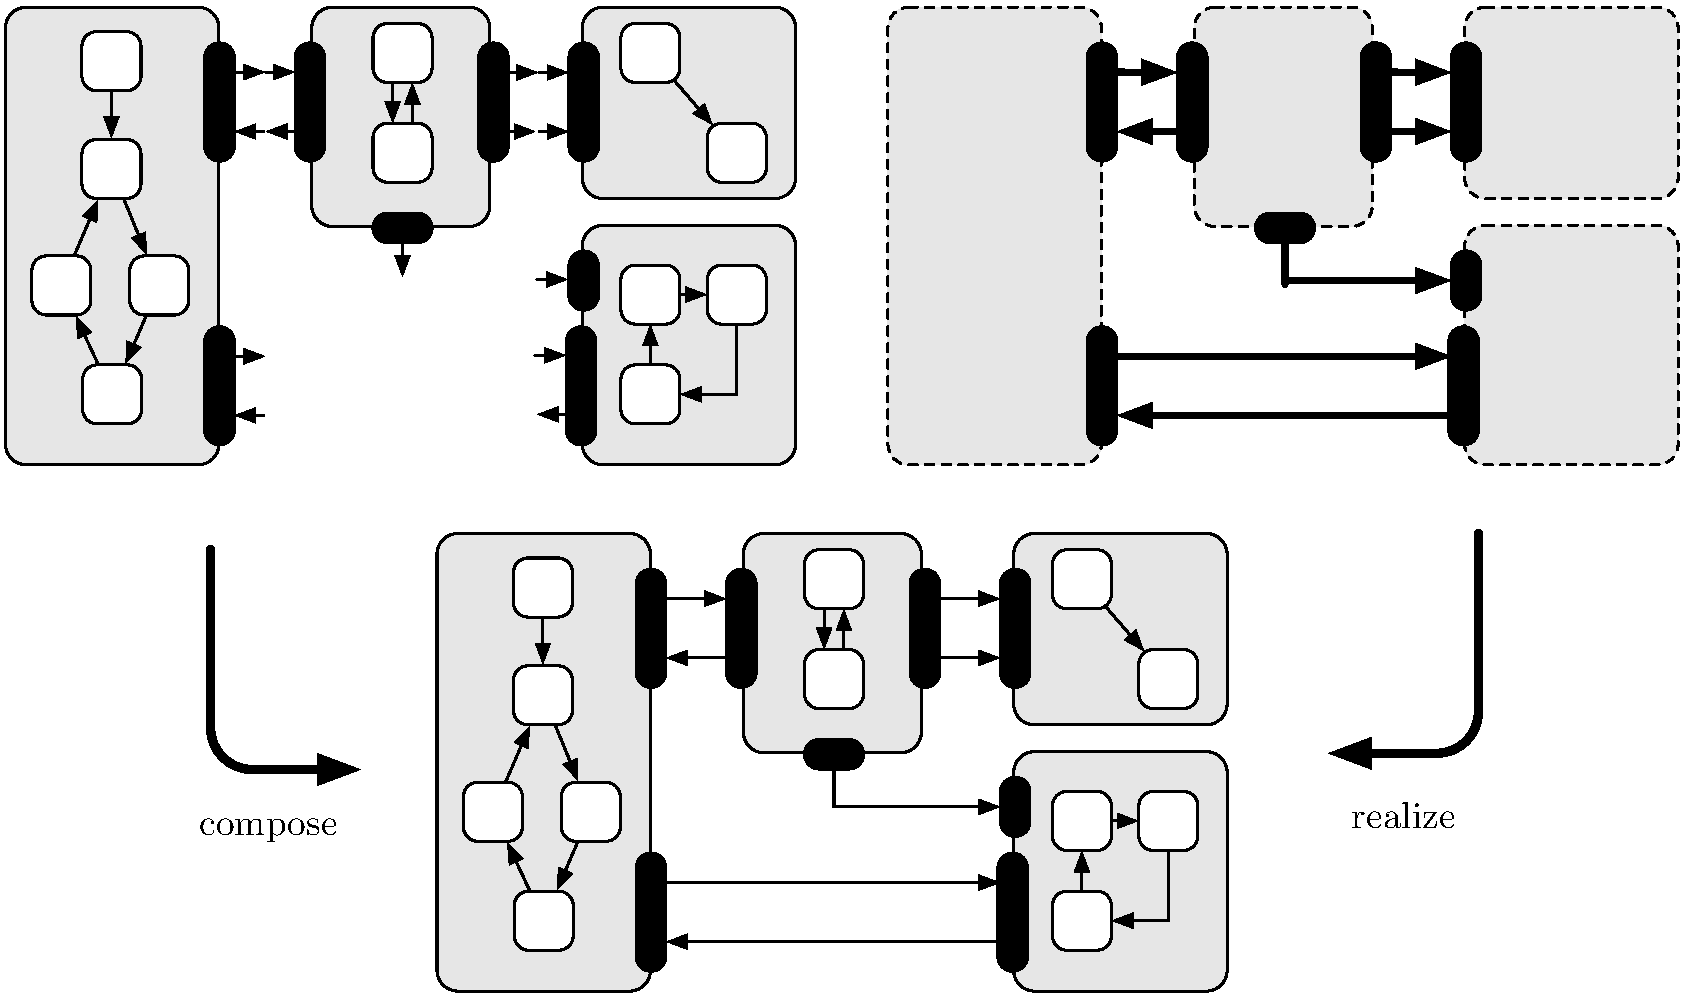
\includegraphics[width=\textwidth]{verification/overview}
\caption{Service choreography.}\label{fig:choreography}
\end{figure}
%%%%%%%%%%%%%%%%%%%%%%%%%%%%%%%%%%%%%%%%%%%%%%%%%%%%%%%%%%%%%%%%%%%%%%%%%%%%%%

In the paradigm of interconnected models (cf.\ \autoref{fig:interconnected}), several local service models are merged into a service choreography; that is, services are composed. This can be seen as bottom-up approach, because the global behavior of the choreography is determined by wiring already specified services. It is the classical scenario of \acronym{SOC} (also called \emph{programming in the large}~\cite{DeRemerK_1976_tse}) facilitating the design of large systems by composing smaller building blocks. The language \bpelchor~\cite{DeckerKLW_2007_icws} has been introduced to specify global interactions by reusing \acronym{WS-BPEL} processes.

\enlargethispage*{\baselineskip}

In contrast, the top-down approach, used by the interaction model paradigm (cf. \autoref{fig:interaction}), starts with a specification of the desired global behavior of a service composition which is yet to be realized. This interaction model is then projected to the participating services and refined toward execution. Interaction modeling aims at early design stages of service compositions and is typically used to model novel interorganizational business processes rather than already established compositions. We shall investigate interaction models in \autoref{chap:realizability}.

\medskip

In this chapter, we investigate the correctness of interconnected models (\ie, service compositions) specified in the language \bpelchor. To this end, we continue as follows. The next section briefly introduces the languages \acronym{WS-BPEL} and \bpelchor. In \autoref{sec:Translation}, we give a formalization of these languages in terms service automata. To facilitate this translation, we employ Petri nets as intermediate formalism, because they offer a compact representation of service automata. \Autoref{sec:Analysis} is devoted to the compatibility analysis of \bpelchor\ choreographies. Experimental results show that the verification techniques scale to choreographies with up to a thousand participants. In \autoref{sec:ver:syn}, the completion of partially specified choreographies is studied. By applying results from previous chapters, we can automatically synthesize stub processes for incomplete choreographies. Finally, \autoref{sec:ver:related} presents related work and \autoref{sec:ver:conclusion} concludes the chapter.





%%%%%%%%%%%%%%%%%%%%%%%%%%%%%%%%%%%%%%%%%%%%%%%%%%%%%%%%%%%%%%%%%%%%%%%%%%%%%%%
\section[WS-BPEL and BPEL4Chor]{WS-BPEL and BPEL{\footnotesize 4}Chor}




%%%%%%%%%%%%%%%%%%%%%%%%%%%%%%%%%%%%%%%%%%%%%%%%%%%%%%%%%%%%%%%%%%%%%%%%%%%%%%
\subsection*{WS-BPEL}

The \emph{Web Services Business Process Execution Language} (\acronym{WS-BPEL}) \cite{standard_bpel}, is a domain-specific language for describing the behavior of business processes based on Web services. This makes \acronym{WS-BPEL} a language for the \emph{programming in the large} paradigm~\cite{DeRemerK_1976_tse}. Its focus is\,---\,unlike modifying variable values in classical programming languages such as C or Java\,---\,the message exchange and interaction with other Web services. Advanced concepts such as instantiation, complex exception handling, and compensation of long running transactions are further features which are needed to implement business processes. These features are first-class citizens in \acronym{WS-BPEL}. In this section, we shall only give a brief overview of those concepts of the language which are relevant in this thesis. The interested reader is referred to detailed introductions \cite{wsbpelprimer,wsbook,AlonsoCKM_2003}.

For the specification of a business process, \acronym{WS-BPEL} provides \emph{activities} and distinguishes between basic and structured activities. A~basic activity can exchange messages with other services (\bpel{invoke}, \bpel{receive}, \bpel{reply}), manipulate and validate data, wait for a period of time or just do nothing (\bpel{empty}), signal faults, invoke a compensation handler, or end the entire process instance.

A structured activity defines a causal execution order on basic activities and can be nested in another structured activity itself. The structured activities include sequential execution (\bpel{sequence}), parallel execution (\bpel{flow}), data-dependent branching (\bpel{if}), timeout- or message-dependent branching (\bpel{pick}), and repeated execution (\bpel{repeatUntil}, \bpel{while}, and \bpel{forEach}). Within activities executed in parallel, the execution order can further be controlled by the usage of \emph{control links}. A control link has a source and a target activity. With Boolean conditions, the splitting and joining behavior can be controlled. If a target activity has to be skipped due to negative evaluation of its join condition, all outgoing control links are set to false, which may cause other activities to be skipped, which is called \emph{dead-path elimination}~\cite{LeymannR_1999_dpe}.

In addition, the structured activity \bpel{scope} links fault, compensation, termination, and event handling to an activity. The \bpel{process} is the outmost scope of the described business process. A \bpel{faultHandler} provides methods to react to faults, which may occur during execution, whereas a \bpel{compensationHandler} can be used to reverse the effects of successfully executed scopes. With the help of an \bpel{eventHandler}, external message events and specified timeouts can be handled. The forced termination of running scopes is controlled by a \bpel{terminationHandler}.

\acronym{WS-BPEL} supports two kind of process specifications. On the one hand, an \emph{executable process} contains all information required to be deployed and executed on a \acronym{WS-BPEL} engine. On the other hand, \acronym{WS-BPEL} further allows to leave parts of the process unspecified. In such \emph{abstract processes}, a placeholder such as an \bpel{opaqueActivity} can be used which is later replaced by concrete activities or branching conditions. An abstract process implicitly specifies a set of executable completions.

Although \acronym{WS-BPEL} is intended as exchange and documentation format, it is based on \acronym{XML} and provides no graphical representation. This makes visualization and specification cumbersome. Hence, every vendor of \acronym{WS-BPEL} development tools introduced proprietary graphical notations. In this thesis, we employ \acronym{BPMN}~\cite{standard_bpmn} as graphical representation. \Autoref{fig:verfication:bpmn} provides an overview of the \acronym{BPMN} constructs used in this thesis. The level of abstraction of \acronym{BPMN} is similar to that of service automata. In particular, the order in which messages are sent and received, the initial state, and final states can be easily derived from a \acronym{BPMN} diagram. In addition, the upcoming \acronym{BPMN} standard~\cite{standard_bpmn2} provides a basic mapping between \acronym{BPMN} and \acronym{WS-BPEL}.

%%%%%%%%%%%%%%%%%%%%%%%%%%%%%%%%%%%%%%%%%%%%%%%%%%%%%%%%%%%%%%%%%%%%%%%%%%%%%%
\begin{figure}[tb]
\centering
{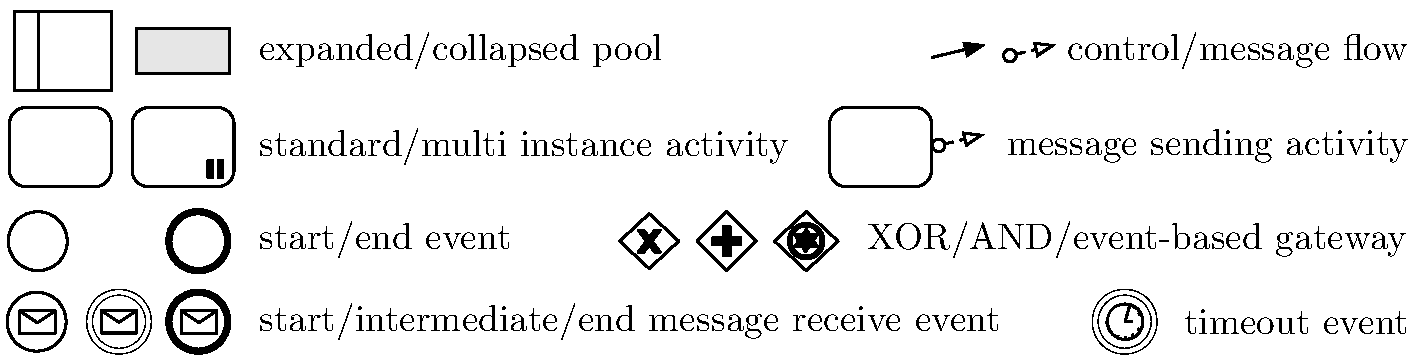
\includegraphics[scale=0.45]{verification/bpmn}}
\caption{\acronym{BPMN} in a nutshell.}\label{fig:verfication:bpmn}
\end{figure}
%%%%%%%%%%%%%%%%%%%%%%%%%%%%%%%%%%%%%%%%%%%%%%%%%%%%%%%%%%%%%%%%%%%%%%%%%%%%%%

%%%%%%%%%%%%%%%%%%%%%%%%%%%%%%%%%%%%%%%%%%%%%%%%%%%%%%%%%%%%%%%%%%%%%%%%%%%%%%
\begin{figure}[tb]
\centering
\subfigure[abstract WS-BPEL process\label{fig:verification:traveler:bpel}]{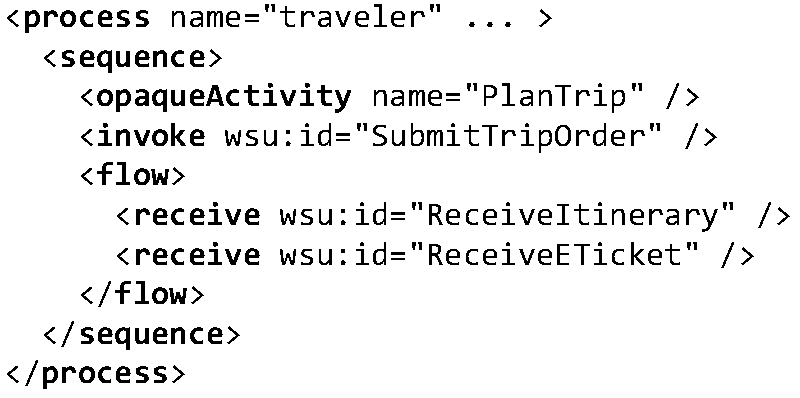
\includegraphics[scale=0.45]{verification/traveler_bpel}}
\subfigure[BPMN visualization\label{fig:verification:traveler:bpmn}]{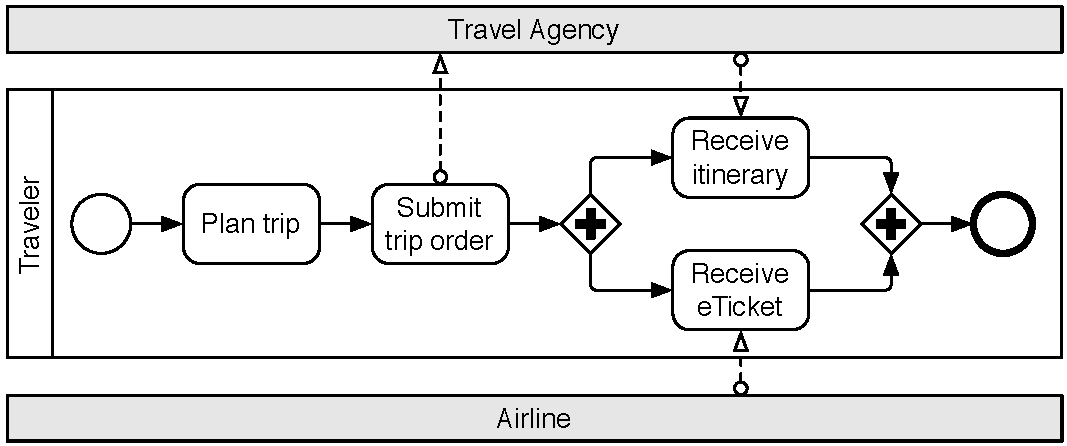
\includegraphics[scale=0.45]{verification/traveler_bpmn}}
\caption{Traveler service.}\label{fig:verification:traveler}
\end{figure}
%%%%%%%%%%%%%%%%%%%%%%%%%%%%%%%%%%%%%%%%%%%%%%%%%%%%%%%%%%%%%%%%%%%%%%%%%%%%%%



\paragraph{Example.}

In this chapter, we investigate a choreography modeling a ticket booking scenario taken from~\cite{DeckerKLW_2007_icws}. It consists of several participants: a \emph{traveler} who sends a trip order (\ie, a request to book a particular trip) to a \emph{travel agency}, which in turn queries several \emph{airline services} for prices and chooses the cheapest offer. Finally, the traveler receives an itinerary from the travel agency and an e-ticket from the chosen airline. \Autoref{fig:verification:traveler:bpel} depicts the traveler's perspective modeled as an abstract \acronym{WS-BPEL} process. In this service orchestration, only the behavior of the traveler is explicitly specified inside an expanded pool, whereas the behavior of the travel agency and the airline services is left unspecified. In \acronym{BPMN} notation, this is modeled by collapsed pools (depicted gray in \autoref{fig:verification:traveler:bpmn}).




%%%%%%%%%%%%%%%%%%%%%%%%%%%%%%%%%%%%%%%%%%%%%%%%%%%%%%%%%%%%%%%%%%%%%%%%%%%%%%
\subsection*{BPEL{\footnotesize 4}Chor}

%%%%%%%%%%%%%%%%%%%%%%%%%%%%%%%%%%%%%%%%%%%%%%%%%%%%%%%%%%%%%%%%%%%%%%%%%%%%%%
\begin{figure}[tb]
\centering
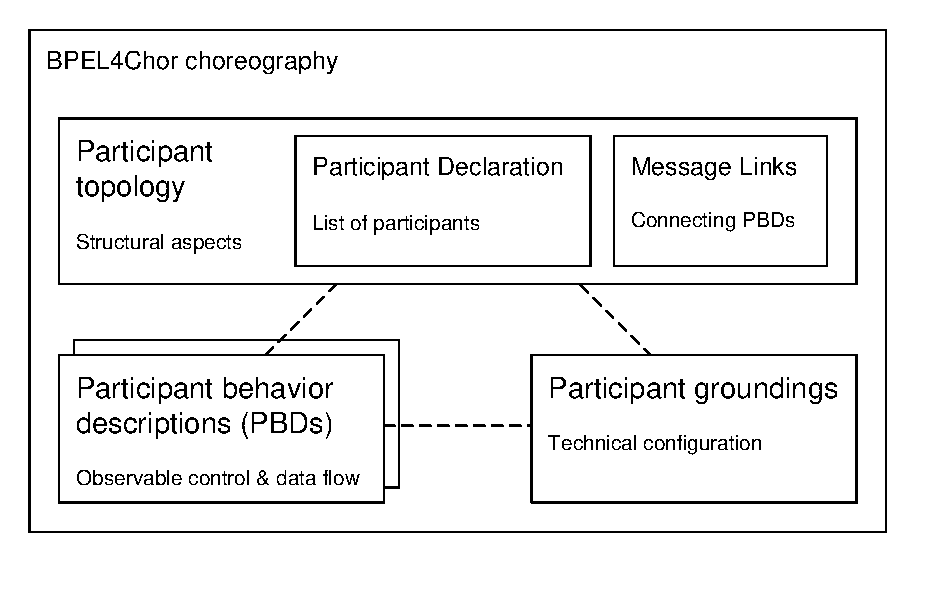
\includegraphics[width=0.7\textwidth]{verification/artifacttypes}
\caption{Artifacts of a \bpelchor{} choreography~\cite{DeckerKLW_2007_icws,DeckerKLW_2009_dke}.}\label{fig:artifacts}
\end{figure}
%%%%%%%%%%%%%%%%%%%%%%%%%%%%%%%%%%%%%%%%%%%%%%%%%%%%%%%%%%%%%%%%%%%%%%%%%%%%%%

%%%%%%%%%%%%%%%%%%%%%%%%%%%%%%%%%%%%%%%%%%%%%%%%%%%%%%%%%%%%%%%%%%%%%%%%%%%%%%
\begin{figure}[tb]
\centering
\includegraphics[width=\textwidth]{verification/translate}
\caption{Workflow from a \bpelchor{} choreography description to executable \acronym{WS-BPEL} processes~\cite{DeckerKLW_2009_dke}.}\label{fig:bpelchortrans}
\end{figure}
%%%%%%%%%%%%%%%%%%%%%%%%%%%%%%%%%%%%%%%%%%%%%%%%%%%%%%%%%%%%%%%%%%%%%%%%%%%%%%

Similar to the traveler service, the other participants' behavior can be specified using \acronym{WS-BPEL}. To describe the interaction of several \acronym{WS-BPEL} processes from a global perspective, \bpelchor{}~\cite{DeckerKLW_2007_icws} has been introduced as a choreography description language based on \acronym{WS-BPEL}. \bpelchor{} is not an execution language, but a means to specify all aspects which are required to execute several \acronym{WS-BPEL} processes as a choreography. This approach aims at reducing complexity by reusing services and execution infrastructure. A choreography described by \bpelchor{} consists of (1)~the \emph{participant topology}, (2) the \emph{participant behavior descriptions} (\acronym{PBD}s), and (3) the \emph{participant groundings} (cf.\ \autoref{fig:artifacts} and \cite{DeckerKLW_2007_icws,DeckerKLW_2009_dke}). The participant topology lists all participants taking part in the choreography and all message links connecting activities of different participants. \bpelchor{} allows for the specification of \emph{participant sets} to group several instances of a participant type. These sets can be (sequentially or parallely) traversed using \acronym{WS-BPEL}'s \bpel{forEach} activity. A \emph{message link} states that a message is sent from the source of the message link to its target. A \bpelchor\ choreography always describes the behavior of all participants. Thus, a \emph{closed world} is assumed.

Every participant has a certain type. For each participant type, a participant behavior description defined in \acronym{WS-BPEL} is given. In this description, port types and operations are omitted and thus the dependency on interface specifications such as \acronym{WSDL}~\cite{standard_wsdl} is removed; that is, the \acronym{PBD}s are abstract \acronym{WS-BPEL} processes. To execute the choreography, every target of a message link has to be grounded to a \acronym{WSDL} operation so that the other participants can use the offered operation. This grounding is done after the choreography design itself, which enables choreography specification reuse. As \acronym{WS-BPEL} is used to specify the behavior of every participant, the development of executable \acronym{WS-BPEL} processes implementing this behavior can be done by using the \acronym{PBD} of a participant as a basis and adding missing details. \citet{ReimannKDL_2008_tr0807} elaborate this process. \Autoref{fig:bpelchortrans} diagrams the overall workflow from a \bpelchor{} choreography to executable \acronym{WS-BPEL} processes. Even though other languages can be used to provide implementations of local behavior, using \acronym{WS-BPEL} is a seamless choice using \bpelchor{}.

\enlargethispage*{2\baselineskip}

\paragraph{Example.}

\Autoref{fig:broken} shows the complete ticket booking scenario from \cite{DeckerKLW_2007_icws}. It specifies the behavior of all participants; that is, all pools are expanded and there is no message exchange with any undefined participants. The multiple airline instances are modeled as follows. The airline pools are stacked and the ``request price'' activity is executed in a multiple instances activity modeling a parallel \bpel{forEach} activity. After receiving a quote from each of the airline instances, a choice is made. Activity ``order tickets'' sends a confirmation message to the selected instance. Finally, a timer event is used to terminate unchosen airline instances.

%%%%%%%%%%%%%%%%%%%%%%%%%%%%%%%%%%%%%%%%%%%%%%%%%%%%%%%%%%%%%%%%%%%%%%%%%%%%%%
\begin{figure}
\centering
\includegraphics[scale=0.45]{verification/choreo}
\caption{Choreography of a ticket booking scenario, taken from~\cite{DeckerKLW_2007_icws}.}\label{fig:broken}
\end{figure}
%%%%%%%%%%%%%%%%%%%%%%%%%%%%%%%%%%%%%%%%%%%%%%%%%%%%%%%%%%%%%%%%%%%%%%%%%%%%%%





%%%%%%%%%%%%%%%%%%%%%%%%%%%%%%%%%%%%%%%%%%%%%%%%%%%%%%%%%%%%%%%%%%%%%%%%%%%%%%%
\section[Formalizing WS-BPEL and BPEL4Chor]{Formalizing WS-BPEL and BPEL{\footnotesize 4}Chor}
\label{sec:Translation}
%%%%%%%%%%%%%%%%%%%%%%%%%%%%%%%%%%%%%%%%%%%%%%%%%%%%%%%%%%%%%%%%%%%%%%%%%%%%%%%

The \acronym{WS-BPEL} language specification~\cite{standard_bpel} describes the operational semantics of \acronym{WS-BPEL} in natural language. This might be sufficient to understand \acronym{WS-BPEL}, but leaves room for ambiguities, contradictions, or unspecified behavior. A formalization~\cite{HinzSS_2005_bpm} of a predecessor specification~\cite{bpel4ws} revealed such unspecified situations which were resolved in the current specification. To \emph{formally} reason about \acronym{WS-BPEL} processes (\ie, to proof or to verify properties), \emph{formal semantics} are needed. Therefore, a lot of work has been conducted to give formal semantics for the behavior of \acronym{WS-BPEL} processes. The approaches cover many formalisms such as Petri nets, automata, abstract state machines, process algebras, and so on~\cite{BreugelK2006,LohmannVOSA_2009_ijbpim,LohmannVD_2008_topnoc}. A few  approaches are feature-complete and try to formalize every aspect of \acronym{WS-BPEL}. These approaches usually aim at a deeper understanding the language. Usually, however, only a subset of a language is formalized to investigate a certain aspect.

In the setting of this thesis, we focus on the \emph{behavior} of a \acronym{WS-BPEL} process. We abstract from other aspects such as time, instantiation, or data. In~\cite{Lohmann_2007_wsfm,Lohmann_2007_hubtr212}, we presented a translation from \acronym{WS-BPEL} to a class of Petri nets. Petri net-based formalisms have the advantage that they are closely related to automata, but can natively express concurrency which facilitates the specification of distributed systems. This make Petri nets an ideal intermediate formalism between \acronym{WS-BPEL} in which concurrency is very common and service automata, the basic formalism of this thesis.




%%%%%%%%%%%%%%%%%%%%%%%%%%%%%%%%%%%%%%%%%%%%%%%%%%%%%%%%%%%%%%%%%%%%%%%%%%%%%%
\subsection*{Petri nets}

\emph{Petri nets}~\cite{Reisig_1985,Murata_1989_pieee} are a formalism which was introduced to model and reason about distributed systems. Locality of the cause and effect of actions are realized consequently. This is reflected by the absence of a global notion of a state in favor of a distribution of resources throughout the system. In addition, Petri nets have a natural graphical representation, which was used as inspiration for later graphical notations such as \acronym{UML} activity diagrams or \acronym{BPMN}.

As already discussed in \autoref{chap:background:discussion}, the algorithm for controllability relies on global states and does not exploit concurrency. To this end, we use service automata as formal model in this thesis. However, Petri nets can be used to compactly represent larger service automata. At the same time, the ability to model distributed systems makes Petri nets a convenient intermediate formalism to translate industrial languages such as \acronym{WS-BPEL} into service automata. 

As Petri nets are not the main topic of this thesis, but just an intermediate formalism, we do not further discuss the specifics of the model, but continue with defining \emph{service nets}, a class of Petri nets, which is tailored to the needs of this chapter. The interested reader is referred to detailed introductions by~\citet{Reisig_1985}, \citet{Murata_1989_pieee}, and \citet{DeselR_1996_pn}.

%%%%%%%%%%%%%%%%%%%%%%%%%%%%%%%%%%%%%%%%%%%%%%%%%%%%%%%%%%%%%%%%%%%%%%%%%%%%%%
\begin{definition}{Service net}%
\label{def:servicenet}%
\nomenclature[N]{$N$}{a service net}%
A \emph{service net} is a tuple $N=[P,T,F,m_0,\Omega,\mathcal{P},\ell]$ such that
\begin{myitemize}
\item $P$ is a finite set of places,
\item $T$ is a finite set of transitions ($P\cap T=\emptyset$),
\item $F\subseteq (P\times T) \cup (T\times P)$ is a flow relation,
\item $m_0\in \Bags(P)$ is an initial marking,
\item $\Omega\subseteq \Bags(P)$ is a set of final markings,
\item $\mathcal{P}$ is an interface, and
\item $\ell: T\rightarrow (\E_\mathcal{P}\cup\{\tau\})$ a labeling function.
\end{myitemize}
\end{definition}
%%%%%%%%%%%%%%%%%%%%%%%%%%%%%%%%%%%%%%%%%%%%%%%%%%%%%%%%%%%%%%%%%%%%%%%%%%%%%%

A service net consists of a classical place/transition net $[P,T,F,m_0]$, a set of final markings, which model desired final states, an interface, and a labeling function that labels each transition with $\tau$ or an event that is derived from the interface.

%%%%%%%%%%%%%%%%%%%%%%%%%%%%%%%%%%%%%%%%%%%%%%%%%%%%%%%%%%%%%%%%%%%%%%%%%%%%%%
\begin{figure}
\centering
\subfigure[$N_1$\label{fig:verification:servicenet}]{\includegraphics[scale=0.45]{verification/n1}}\hfill
\subfigure[$N_1$ after firing $t_{1}$\label{fig:verification:servicenet1}]{\includegraphics[scale=0.45]{verification/n1-1}}\hfill
\subfigure[$A_{N_1}$\label{fig:verification:servicenetsa}]{\includegraphics[scale=0.45]{verification/san1}}
\caption{A service net with $\Omega=\{\mset{p_{4},p_{5},p_{5}}\}$ (a) whose initial marking $m_{0}=[p_{1}]$ enables transition $t_{1}$. Firing~$t_{1}$ yields the marking $[p_{2},p_{3}]$~(b). The net can be translated into a service automaton~(c).}
\end{figure}
%%%%%%%%%%%%%%%%%%%%%%%%%%%%%%%%%%%%%%%%%%%%%%%%%%%%%%%%%%%%%%%%%%%%%%%%%%%%%%

We use the standard graphical notation for Petri nets and depict places by circles, transitions by rectangles, and the flow relation by directed arcs. A marking $m$ is represented by a distribution of $m(p)$ black dots (called ``tokens'') to each place $p$. Transition labels are written inside the transitions. Final markings have no graphical representation and are annotated to the net. We depict ports in the same way as for service automata. \Autoref{fig:verification:servicenet} shows an example.

\Autoref{def:servicenet} already suggests a close syntactical relationship to service automata. To give a mapping from a service net to a service automaton, we need to define the operational semantics of a service net; that is, we define a concept of states and state transitions. We do this by applying definitions known from place/transition nets.

%%%%%%%%%%%%%%%%%%%%%%%%%%%%%%%%%%%%%%%%%%%%%%%%%%%%%%%%%%%%%%%%%%%%%%%%%%%%%%
\begin{definition}{Firing rule}
\nomenclature[mtm]{$m \mathrel{[t\rangle}_N m'$}{firing transition $t$ in marking $m$ resulting marking $m'$}%
Let $N=[P,T,F,m_0,\Omega,\mathcal{P},\ell]$ be a service net. For a node $x\in P\cup T$, define the preset of $x$ as ${}^\bullet x:=\{y\mid [y,x]\in F\}$ and the postset of $x$ as $x^\bullet:=\{y\mid [x,y]\in F\}$.

A transition $t$ is \define{enabled} at marking $m\in\Bags(P)$ iff $m(p)>0$ holds for all places $p \in {}^\bullet x$. An enabled transition $t$ can \define{fire} in $m$, denoted $m \mathrel{[t\rangle}_N m'$, yielding the successor marking $m'$ with\vspace{-0.5em}
$$m'(p):=\begin{cases}
m(p)-1,&\text{iff $p\in {}^\bullet t \setminus t^\bullet$,}\\
m(p)+1,&\text{iff $p\in t^\bullet \setminus {}^\bullet t$,}\\
m(p),&\text{otherwise.}\end{cases}$$\vspace{-1em}
\end{definition}
%%%%%%%%%%%%%%%%%%%%%%%%%%%%%%%%%%%%%%%%%%%%%%%%%%%%%%%%%%%%%%%%%%%%%%%%%%%%%%

In the net of \autoref{fig:verification:servicenet}, transition $t_{1}$ is enabled in the initial marking. Firing $t_{1}$ yields a successor marking depicted in \autoref{fig:verification:servicenet1}. Now we can use markings of a service net as states of a service automaton. Likewise, the labeling of the service net's transitions can be used to derive a labeled transition relation.

%%%%%%%%%%%%%%%%%%%%%%%%%%%%%%%%%%%%%%%%%%%%%%%%%%%%%%%%%%%%%%%%%%%%%%%%%%%%%%
\begin{definition}{Service net translation into service automaton}
\nomenclature[AN]{$A_{N}$}{the translation of service net $N$ to a service automaton}%
Let $N=[P,T,F,m_0,\Omega,\mathcal{P},\ell]$ be a service net. Define the service automaton for $N$ as $A_N:=[Q,q_0,{\shortrightarrow},\Omega,\mathcal{P}]$ with
\begin{myitemize}
\item $Q:=\Bags(P)$,
\item $q_0 := m_0$, and
\item ${\shortrightarrow} := \{ [m,\ell(t),m'] \mid m \mathrel{[t\rangle}_N m' \}$.
\end{myitemize}
\end{definition}
%%%%%%%%%%%%%%%%%%%%%%%%%%%%%%%%%%%%%%%%%%%%%%%%%%%%%%%%%%%%%%%%%%%%%%%%%%%%%%

As always, we only consider reachable states of $A_N$. \Autoref{fig:verification:servicenetsa} depicts the service automaton for the service net of \autoref{fig:verification:servicenet}. Even though the transitions $t_{2}$ and $t_{3}$ can fire concurrently in $N_1$, they are explicitly ordered in $A_{N_1}$ which results in several intermediate states. This potential exponential growth of intermediate states in the size of the net is referred to as the \emph{state explosion problem}~\cite{Valmari_1996_pn}.




%%%%%%%%%%%%%%%%%%%%%%%%%%%%%%%%%%%%%%%%%%%%%%%%%%%%%%%%%%%%%%%%%%%%%%%%%%%%%%
\subsection*{Formal Semantics for WS-BPEL}

In the following, we use service nets to define formal semantics for \acronym{WS-BPEL}. The translation of a \acronym{WS-BPEL} process into a service net model is guided by the syntax of \acronym{WS-BPEL}. In \acronym{WS-BPEL}, a process is built by plugging instances of language constructs together. Accordingly, each construct of the language is translated separately into a service net. Such a net forms a \emph{pattern} of the respective \acronym{WS-BPEL} construct. Each pattern has an interface for joining it with other patterns as is done with \acronym{WS-BPEL} constructs. Patterns capturing \acronym{WS-BPEL}'s structured activities may carry any number of inner patterns as its equivalent in \acronym{WS-BPEL} can do. The collection of patterns forms the \emph{service net semantics} for \acronym{WS-BPEL}.

%%%%%%%%%%%%%%%%%%%%%%%%%%%%%%%%%%%%%%%%%%%%%%%%%%%%%%%%%%%%%%%%%%%%%%%%%%%%%%
\begin{figure}
\centering
\includegraphics[scale=0.45]{verification/bpel}
\caption{Petri net patterns to formalize \acronym{WS-BPEL}.}\label{fig:bpel}
\end{figure}
%%%%%%%%%%%%%%%%%%%%%%%%%%%%%%%%%%%%%%%%%%%%%%%%%%%%%%%%%%%%%%%%%%%%%%%%%%%%%%

Whereas the original semantics~\cite{Lohmann_2007_wsfm,Lohmann_2007_hubtr212} captures the standard as well as the exceptional behavior of a \acronym{WS-BPEL} process, we only consider the standard behavior in this thesis to ease the presentation. We also do not present the formalization of control links and dead-path elimination. \Autoref{fig:bpel} gives an overview of the used patterns. These patterns can, however, be canonically enhanced to model fault, compensation, and exception handling of the participating \acronym{WS-BPEL} processes. The translation is guided by the structure of \acronym{WS-BPEL} and first translates the basic activities into the respective Petri net patterns. These nets are then embedded into those patterns structured activities. The interested reader is referred to a report~\cite{Lohmann_2007_hubtr212} which discusses the complete semantics as it is implemented in the tool \bpelowfn.

%%%%%%%%%%%%%%%%%%%%%%%%%%%%%%%%%%%%%%%%%%%%%%%%%%%%%%%%%%%%%%%%%%%%%%%%%%%%%%
\begin{figure}[tb]
\centering
\subfigure[service net with $\Omega=\{\mset{p_{\omega}}\}$\label{fig:verification:travelerpn}]{\makebox[0.49\textwidth]{\includegraphics[scale=0.45]{verification/travelerpn}}}\hfill
\subfigure[corresponding service automaton\label{fig:verification:travelersa}]{\makebox[0.49\textwidth]{\includegraphics[scale=0.45]{verification/travelersa}}}
%\includegraphics[scale=0.45]{verification/bpel}
\caption{Translation of the \acronym{WS-BPEL} traveler service.}\label{fig:verification:travelerpnsa}
\end{figure}
%%%%%%%%%%%%%%%%%%%%%%%%%%%%%%%%%%%%%%%%%%%%%%%%%%%%%%%%%%%%%%%%%%%%%%%%%%%%%%


\paragraph{Example.}

\Autoref{fig:verification:travelerpn} depicts the traveler service from \autoref{fig:verification:traveler} translated into a service net. From this net, a service automaton (cf.\ \autoref{fig:verification:travelersa}) can be canonically derived.




%%%%%%%%%%%%%%%%%%%%%%%%%%%%%%%%%%%%%%%%%%%%%%%%%%%%%%%%%%%%%%%%%%%%%%%%%%%%%%
\subsection*{Petri Net Semantics for BPEL{\footnotesize 4}Chor}

To translate a \bpelchor{} choreography, two steps are involved: (1) translate each participant's \acronym{WS-BPEL} process into a service automaton and (2) compose the resulting models. All required information can be derived from the \bpelchor{} choreography, cf.~\autoref{fig:artifacts}. In the ticket booking scenario we use as running example, however, there are several \emph{instances} of the airline service involved. To this end, the translation described in \cite{Lohmann_2007_wsfm,Lohmann_2007_hubtr212} needs to be extended to support multiple \emph{instantiation} of participants.

With ``instantiation'' we do not refer to the lifecycle of a service instance. This lifecycle includes the analysis of incoming messages to decide whether a new instance needs to be created or messages need to be forwarded to existing instances (called \emph{correlation} in \acronym{WS-BPEL}) and the removal of terminated instances from the execution engine. These steps are realized transparently by execution languages such as \acronym{WS-BPEL} and should not influence the behavior of a service composition. In the translation, ``instantiation'' means  creating several copies of a participants and adjusting the wiring of interfaces.

We realized the instantiation of a choreography participant by providing several identical copies of the service net of the participant description. By choosing unique place and transition names (\eg, using prefixes) the behavior of each instance is distinctively modeled. To be able to later compose these models, also the message channel names need to be adjusted to ensure bilateral and unidirectional communication. Therefore, we need to adjust the participant's behavior according to the following scenarios:

\begin{niceenumerate}
\item A message is exchanged between two uninstantiated participants (\eg, the trip order sent by the traveler to the agency): no adjustment is needed.

\item A message is exchanged between an uninstantiated participant and one particular instantiated participant (\eg, the price request sent by the agency to each airline instance): The behavior of the uninstantiated participant needs to be duplicated and executed for each instance, either concurrently or sequentially depending on the \bpel{forEach} activity used to traverse the instances. In addition, the message channel names need to be adjusted.

\item A message is exchanged between an uninstantiated participant and an arbitrary chosen instantiated participant (\eg, the e-ticket sent by the selected airline to the traveler): The behavior of the uninstantiated participant needs to be duplicated for each instance and executed mutually exclusively. In addition, the message channel names need to be adjusted.

\item A message is exchanged between two instantiated participants (not pre\-sent in our example choreography): Similar to the second scenario.
\end{niceenumerate}

As stated earlier, the participant topology holds the necessary information about which process and which message channel has to be instantiated. Admittedly, the topology does not provide the number of instances of each participant. \emph{We therefore demand an upper bound of instances to be specified for each participant set.} Whereas this upper bound may not be necessary if \bpelchor{} is just a means to \emph{describe} choreographies, its definition is reasonable if such a choreography should be \emph{analyzed} or \emph{executed}.

%%%%%%%%%%%%%%%%%%%%%%%%%%%%%%%%%%%%%%%%%%%%%%%%%%%%%%%%%%%%%%%%%%%%%%%%%%%%%%
\begin{figure}%[t!]
\centering
\subfigure[\label{fig:code} code snippet of the agency process]{\makebox[6cm]{\includegraphics[scale=0.45]{verification/code}}}
\hfill
\subfigure[\label{fig:agency} resulting subnet of the agency]{\makebox[0.49\textwidth]{\includegraphics[scale=0.45]{verification/snippet_net}}}\subfigure[\label{fig:agencysa} resulting part as service automaton]{\makebox[0.49\textwidth]{\includegraphics[scale=0.45]{verification/snippet_sa}}}
\caption{Example for the instantiation for two airline instances. The \acronym{WS-BPEL} process of the agency (a) translated into a Petri net (b) and a service automaton (c). }
\label{fig:instantiation}
\end{figure}
%%%%%%%%%%%%%%%%%%%%%%%%%%%%%%%%%%%%%%%%%%%%%%%%%%%%%%%%%%%%%%%%%%%%%%%%%%%%%%


\paragraph{Example.}

For an example of these scenarios, consider the \acronym{WS-BPEL} code snippet of the agency process depicted in \autoref{fig:code}. For two airline instances, \Autoref{fig:agency} depicts the resulting subnet. The trip order message ($o$) sent by the traveler to the agency is an example of the first scenario, as both services (traveler and agency) are uninstantiated. Therefore, the receipt of the trip order message is modeled by a single transition. The price request ($p_{1}$ and $p_{2}$) sent to and the corresponding price quotes ($q_{1}$ and $q_{2}$) received from the airline instances are examples for the second scenario. Therefore, the communicating transitions are instantiated, resulting in renamed message channel names. As specified by the parallel \bpel{forEach} activity, the agency communicates concurrently with each airline. The ticket order sent to only one airline instance ($t_{1}$ and $t_{2}$) is an example for the third scenario.




%%%%%%%%%%%%%%%%%%%%%%%%%%%%%%%%%%%%%%%%%%%%%%%%%%%%%%%%%%%%%%%%%%%%%%%%%%%%%%
\subsection*{Translating the example choreography}

The presented translation approach is implemented in our compiler \bpelowfn{} \cite{Lohmann_2007_hubtr212}. \bpelowfn\ enables us to automatically translate \acronym{WS-BPEL} choreographies into service net models. We translated the example choreography with 10 airline instances into a Petri net, cf.~\autoref{fig:choreography10}. The resulting net has 188 places and 151 transitions. Standard structural reduction techniques~\cite{Murata_1989_pieee} simplified the net to 113 places and 76 transitions while preserving compatibility.

%%%%%%%%%%%%%%%%%%%%%%%%%%%%%%%%%%%%%%%%%%%%%%%%%%%%%%%%%%%%%%%%%%%%%%%%%%%%%%
\begin{figure}[tb]
\centering
\includegraphics[width=0.9\textwidth]{verification/choreography10}
\caption{Service composition with 10 airline instances translated into a service net using the compiler \bpelowfn.}\label{fig:choreography10}%
\end{figure}
%%%%%%%%%%%%%%%%%%%%%%%%%%%%%%%%%%%%%%%%%%%%%%%%%%%%%%%%%%%%%%%%%%%%%%%%%%%%%%

In practice, we do not translate the intermediate \acronym{WS-BPEL} services into service automata, but compose the intermediate service nets. The definition of this service net composition operator is a straightforward adaption of \autoref{def:composition}; \citet{Wolf_2007_sa} provides a formal definition.





%%%%%%%%%%%%%%%%%%%%%%%%%%%%%%%%%%%%%%%%%%%%%%%%%%%%%%%%%%%%%%%%%%%%%%%%%%%%%%%
\section{Analyzing closed choreographies}\label{sec:Analysis}
%%%%%%%%%%%%%%%%%%%%%%%%%%%%%%%%%%%%%%%%%%%%%%%%%%%%%%%%%%%%%%%%%%%%%%%%%%%%%%%

A \bpelchor{} choreography description specifies not only the behavior of each participant, but also their interaction. In addition, the \mbox{closed-world} assumption ensures that there is no further entity influencing the behavior of the participants. As a result, a complete \bpelchor{} choreography description can be translated into a closed service automaton (\ie, a service automaton with closed interface). Such a closed system can be analyzed without the necessity of taking an environment into account.

The correctness of a \bpelchor{} choreography is crucial, because it is the basis for technical groundings as well as manual refinement (cf.~\autoref{fig:bpelchortrans}). By checking this \bpelchor{} choreography, we can rule out errors well before refinement, implementation, and deployment.

As motivated in \autoref{chap:formal}, we employ compatibility as central correctness criterion for closed service compositions. It allows us to derive more elaborate concepts such as controllability, behavioral constraints, or operating guidelines. Beside compatibility, temporal logics allow to express several other properties of closed systems which can be investigated using standard model checking tools~\cite{ClarkeGD_1999_book,BaierK_2008_book}. Interesting questions include:

\begin{niceitemize}
\item Will a certain activity of a participant be executed?

\item Does there exist a state in which more than one message is pending on a communication channel? 

\item What is the minimal/maximal number of messages to be sent to reach a final state of the choreography?

\item Will a participant always receive an answer? Can a participant enforce the receipt of a certain message?
\end{niceitemize}

These properties focus on closed systems and are not applicable to open systems in which an environment has to be taken into account. In this situation, the application of behavioral constraints (cf.~\autoref{chap:validation}) may help to investigate and validate the participants' behavior, but the results cannot be straightforwardly mapped back to the original \acronym{WS-BPEL} or \bpelchor{} model.




%%%%%%%%%%%%%%%%%%%%%%%%%%%%%%%%%%%%%%%%%%%%%%%%%%%%%%%%%%%%%%%%%%%%%%%%%%%%%%
\subsection*{Analyzing the example choreography}

We analyzed the Petri net model of Sect.~\ref{sec:Translation} with the Petri net verification tool LoLA~\cite{Schmidt_2000_icatpn,Wolf_2007_icatpn}, a state-of-the-art model checker which implements several state space reduction techniques. The unreduced state space consists of 9{,}806{,}583 states. Using LoLA, we detected a deadlock in the model. We could map this deadlocking state of the model back to the participating services with the help of a \emph{witness path}. The deadlock occurs, if the agency's choice for an airline takes too much time or if the message sent to the chosen airline is delayed. In this case, the timeout (\ie, the \bpel{onAlarm} branch) of \emph{all} participating airlines ends their instances and the agency deadlocks waiting for a confirmation message from the chosen airline.

Even though the presented example does not have the complexity of industrial service choreographies, the design flaw is very subtle and was not detected by the authors of the paper~\cite{DeckerKLW_2007_icws}, where the example was taken from. Admittedly, our formalization abstracted from time and models timer-based decisions by nondeterminism. Nevertheless, the detected deadlock models a situation in which all airline instances time out, which may happen independently of a concretely chosen timeout interval. In addition, the latency of messages is hard to predict when asynchronous message transfer over the Internet is used to interact.




%%%%%%%%%%%%%%%%%%%%%%%%%%%%%%%%%%%%%%%%%%%%%%%%%%%%%%%%%%%%%%%%%%%%%%%%%%%%%%
\subsection*{Correcting the example choreography}

There are many ways to correct the deadlocking choreography. A straightforward attempt would be to replace the airline service's timeout by a message sent by the agency, which explicitly informs all but one airline that their price quote was not chosen. This would, however, add an unrealistic dependency between the agency and all running airline instances. To this end, we decided to keep the timeout, but at the same time ensure a response of the airline service even if a ticket order is received after the timeout.

%%%%%%%%%%%%%%%%%%%%%%%%%%%%%%%%%%%%%%%%%%%%%%%%%%%%%%%%%%%%%%%%%%%%%%%%%%%%%%
\begin{figure}
\centering
\includegraphics[scale=0.45]{verification/choreo-fix}
\caption{Fixed choreography of the ticket booking scenario. The two start events at the airline process denote a \acronym{WS-BPEL} \bpel{pick} activity.} \label{fig:fixed}
\end{figure}
%%%%%%%%%%%%%%%%%%%%%%%%%%%%%%%%%%%%%%%%%%%%%%%%%%%%%%%%%%%%%%%%%%%%%%%%%%%%%%

Hence, we changed the choreography as follows (cf.~gray shapes in \autoref{fig:fixed}). The airline's behavior does not change if the agency's ticket order is received before the timeout occurred and if the timeout occurs, the airline service's instance still terminates. However, a new branch was added to the airline: \emph{this branch models the situation in which the agency's ticket order is received after the timeout. In this case, the airline service is restarted and the ticket order is rejected.} In addition, the services of the agency and the traveler are adjusted to handle the case in which all airlines time out and no ticket could be booked.

Note that \acronym{BPMN} can only specify message flow between exactly two activities and does not support the concept of message channels. In the fixed choreography however, the ticket order sent by the agency can be received by two message events of the airline. We denote this in \autoref{fig:fixed} by a branching message flow originating in the ``order tickets'' activity of the travel agency.




%%%%%%%%%%%%%%%%%%%%%%%%%%%%%%%%%%%%%%%%%%%%%%%%%%%%%%%%%%%%%%%%%%%%%%%%%%%%%%
\subsection*{Analyzing the fixed example choreography}

We translated the fixed choreography with five airline instances into a Petri net model. Because of the newly introduced activities, its structure and its state space have grown. The resulting (structurally reduced) net has 113 places and 97 transitions. The model has 9{,}805{,}560 states and is now compatible.

\medskip

The correction is nontrivial and possibly error-prone. To ensure compatibility, an additional check is needed. In the next chapter, we shall provide an algorithm to automatically suggest corrections for incorrect choreographies.



%%%%%%%%%%%%%%%%%%%%%%%%%%%%%%%%%%%%%%%%%%%%%%%%%%%%%%%%%%%%%%%%%%%%%%%%%%%%%%%
\subsection*{Experimental results}

In the previous sections, we analyzed the first and the second choreography (cf.~\autoref{fig:broken} and \autoref{fig:fixed}, resp.) with five airline instances. For these five airlines, the resulting models already had more than 3{,}000 states. The states space grows dramatically when the number of airlines is further increased (cf.~\autoref{tab:verification_sizes}). For ten airlines, the model has over nine million states, and for larger numbers, the full state space could not be constructed due to memory overflow (denoted by ``---'' in \autoref{tab:verification_sizes}). The experiments conducted using a computer with 2 gigabytes of memory.

%%%%%%%%%%%%%%%%%%%%%%%%%%%%%%%%%%%%%%%%%%%%%%%%%%%%%%%%%%%%%%%%%%%%%%%%%%%%%%
\begin{table}
\centering
\caption{Experimental results for compatibility check using LoLA.}
\medskip
\label{tab:verification_sizes}
first example, cf.~\autoref{fig:broken} \footnotesize
\begin{tabular*}{\textwidth}{@{\extracolsep{\fill}}lrrrrr}
\toprule
airline instances & $1$ & $5$ & $10$ & $100$ & $1{,}000$\\ \midrule
net places & $20$ & $63$ & $113$ & $1{,}013$ & $10{,}013$ \\
net transitions & $10$ & $41$ & $76$ & $706$ & $7.006$ \\ \midrule
states (unreduced) & $14$ & $3{,}483$ & $9{,}806{,}583$ & --- & ---  \\
states (symmetry) & $14$ & $561$ & $378{,}096$ & --- & ---  \\
states (POR) & $11$ & $86$ & $261$ & $18{,}061$ & $1{,}752{,}867$  \\
states (POR + symmetry) & $11$ & $30$ & $50$ & $410$ & $4{,}010$  \\
\bottomrule
\end{tabular*}
\medskip\\
\normalsize second example, cf.~\autoref{fig:fixed}\\ \footnotesize
\begin{tabular*}{\textwidth}{@{\extracolsep{\fill}}lrrrrr}
\toprule
airline instances & $1$ & $5$ & $10$ & $100$ & $1{,}000$ \\ \midrule
net places & $19$ & $63$ & $113$ & $1{,}013$ & $10{,}113$ \\
net transitions & $12$ & $52$ & $97$ & $907$ & $9{,}007$ \\ \midrule
states (unreduced) & $13$ & $3{,}812$ & $9{,}805{,}560$ & --- & --- \\
states (symmetry) & $13$ & $704$ & $329{,}996$ & --- & --- \\
states (POR) & $12$ & $88$ & $228$ & $8{,}361$ & $734{,}049$ \\
states (POR + symmetry) & $12$ & $28$ & $43$ & $314$ & $3{,}014$ \\
\bottomrule
\end{tabular*}
\end{table}
%%%%%%%%%%%%%%%%%%%%%%%%%%%%%%%%%%%%%%%%%%%%%%%%%%%%%%%%%%%%%%%%%%%%%%%%%%%%%%

However, several state space reduction techniques can be applied to reduce the size of the state space while still being able to analyze desired properties such as deadlock-freedom. In our particular example, we applied \emph{symmetry reduction} and \emph{partial order reduction}, both implemented in LoLA (\citet{Wolf_2007_icatpn} provides further references). The symmetry reduction exploits  that all airline instances have the same structure. This regular structure induces symmetries on the net structure itself, but also on the state space of the choreography. Intuitively, the instances of the airline service act ``similar'' or ``symmetric''. During the state space construction, symmetric states are merged. The partial order reduction follows a different approach: As all instances run concurrently, any order of transitions of the airline instances are represented in the state space. These transition sequences introduce an exponential number of intermediate states, resulting in state space explosion. However, the actual order of independent actions is not relevant to detect deadlocks, for instance. To this end, partial order reduction tries to only construct a single transition sequence of transitions of different airline instances to ease the state space explosion.

\enlargethispage*{\baselineskip}

In case each of the reduction technique is applied in isolation, the number of states grows more slowly, yet still exponentially in the number of airline instances. The combination of both techniques, however, yields a linear increase of states (cf.~\autoref{tab:verification_sizes}). Hence, we are able to verify properties of \acronym{WS-BPEL} choreographies with thousands of participating services. This shows that the presented approach should be likewise suitable to analyze real-life examples. The numbers show that the correction of the model only yields few additional states.





%%%%%%%%%%%%%%%%%%%%%%%%%%%%%%%%%%%%%%%%%%%%%%%%%%%%%%%%%%%%%%%%%%%%%%%%%%%%%%%
\section{Completing Choreographies}\label{sec:ver:syn}
%%%%%%%%%%%%%%%%%%%%%%%%%%%%%%%%%%%%%%%%%%%%%%%%%%%%%%%%%%%%%%%%%%%%%%%%%%%%%%%

While the analysis of closed choreographies may help to find errors such as deadlocks in the interaction between the participating services, service automata may also support the \emph{design} of choreographies. A choreography in which one participating service is missing can, for instance, be \emph{completed} by automatically synthesizing the missing participant service. This synthesized service is then guaranteed to communicate compatibly with the other participants. To this end, controllability is an important property. In~\autoref{chap:formal}, we presented an algorithm to constructively decide controllability of an open service automaton. This algorithm is implemented in the tool Wendy~\cite{LohmannW_2009_wendy}. If a partner exists such that the composition is compatible, it is automatically generated.




%%%%%%%%%%%%%%%%%%%%%%%%%%%%%%%%%%%%%%%%%%%%%%%%%%%%%%%%%%%%%%%%%%%%%%%%%%%%%%
\subsection*{Synthesizing a traveler participant}

Consider again the fixed choreography of \autoref{fig:fixed}. If, for example, only the services of the agency and the airlines were specified, the blueprint of a traveler participant could be synthesized. If such a service exists (\ie, the composition of the existing services is controllable), it completes the choreography which is then compatible by construction. To this end, the incomplete choreography is translated into a service net using \bpelowfn. This service automaton is then analyzed by Wendy. If the service automaton is controllable, a service automaton modeling the behavior of a partner service is synthesized.

%%%%%%%%%%%%%%%%%%%%%%%%%%%%%%%%%%%%%%%%%%%%%%%%%%%%%%%%%%%%%%%%%%%%%%%%%%%%%%
\begin{figure}[tb]
\centering
\subfigure[synthesized traveler\label{fig:synthesized_traveler}]{\makebox[0.45\textwidth]{\includegraphics[scale=0.45]{verification/syn_traveler}}}\hfill
\subfigure[two synthesized airline instances\label{fig:synthesized_airlines}]{\makebox[0.45\textwidth]{\includegraphics[scale=0.45]{verification/syn_airline}}}
\caption{Participant services synthesized to complete the example choreography.}
\end{figure}
%%%%%%%%%%%%%%%%%%%%%%%%%%%%%%%%%%%%%%%%%%%%%%%%%%%%%%%%%%%%%%%%%%%%%%%%%%%%%%


\paragraph{Example.}

\Autoref{fig:synthesized_traveler} depicts the synthesized service automaton of a traveler participant which completes the choreography. This traveler participant slightly differs from the traveler participant in the repaired choreography (cf.~\autoref{fig:fixed}). First, there exists no transition modeling the planning of the trip, because such a transition is internal (\ie, not communicating), but the participant was synthesized based on the external behavior; that is, only the interaction of the service was taken into account. Second, the itinerary and the e-ticket can be received in any order. For example, it would be possible to swap the two receive events in~\autoref{fig:fixed}. This is because of the asynchronous communication model: messages can keep pending on the interface, so there is no order in which they have to be received. From this service automaton, an abstract \acronym{WS-BPEL} process can be derived using existing approaches~\cite{LassenA_2006_otm,AalstL_2008_ist,LohmannK_2008_mod}. As this translation is out of scope of this thesis, we do not present it here.




%%%%%%%%%%%%%%%%%%%%%%%%%%%%%%%%%%%%%%%%%%%%%%%%%%%%%%%%%%%%%%%%%%%%%%%%%%%%%%
\subsection*{Experimental results}

To investigate the applicability of the synthesis algorithm in this scenario, we conducted the following experiment. We fixed the travel agency and synthesized the traveler service for different numbers of airline instances.

\Autoref{tab:syn} summarizes the results. The first two lines list the size of the structurally reduced service net modeling the composition of the airline instances and the travel agency. The next line lists the number of states of this open composition; that is, the size of the service automaton that is checked for controllability. The next two lines give information on the size of the synthesized traveler service. Finally, the time consumption of the synthesis is listed. With our test setup of 2 gigabytes of memory and a 3 \acronym{GH}z processor, we were able to synthesize a traveler service for up to 14 airline instances. For this number, the service automaton modeling the composition of the travel agency and the airline instances has already more than five million states and the synthesis took more than six minutes.

%%%%%%%%%%%%%%%%%%%%%%%%%%%%%%%%%%%%%%%%%%%%%%%%%%%%%%%%%%%%%%%%%%%%%%%%%%%%%%
\begin{table}
\centering
\caption{Experimental results for participant synthesis using Wendy.}
\medskip
\label{tab:syn}
\footnotesize
\begin{tabular*}{\textwidth}{@{\extracolsep{\fill}}lrrrrrr}
\toprule
airline instances  & $4$ & $6$ & $8$ & $10$ & $12$ & $14$ \\ \midrule
net places       & $35$ & $49$ & $63$ & $77$ & $91$ & $105$ \\
net transitions  &$18$ & $26$ & $34$& $42$& $50$& $58$  \\
states  & $176$ & $1{,}240$ & $9{,}120$ & $71{,}366$ & $588{,}784$ & $5{,}045{,}112$ \\ \midrule
synthesized states  & $11$ & $15$ & $19$ & $23$ & $27$ & $31$\\
synthesized transitions  & $56$ & $106$ & $172$ & $254$ & $352$ & $466$ \\
synthesis time [s] & $0$& $0$ & $0$ & $3$ & $36$ & $378$ \\
\bottomrule
\end{tabular*}
\end{table}
%%%%%%%%%%%%%%%%%%%%%%%%%%%%%%%%%%%%%%%%%%%%%%%%%%%%%%%%%%%%%%%%%%%%%%%%%%%%%%

Compared with the compatibility analysis (cf.~\autoref{tab:verification_sizes}), the synthesis problem does not scale well with respect to the number of airline instances that can be processed (14 vs.\ 1{,}000). This is because we currently do not apply state space reduction techniques. Hence, the size of the service automaton to be considered suffers from state explosion and grows exponentially in the number of the airline instances. However, without these techniques, also the compatibility analysis becomes unfeasible if the size of the state space exceeds about 10 million states.

The experiment also shows that just a small number of asynchronously communicating participants are enough to result in an open system which has much more states than industrial Web services (cf.~\autoref{tab:synthesis}). For the ticket booking scenario, the composition of a travel agency and ten airline instances has already four times more states than the largest service automaton we considered in~\autoref{tab:synthesis}.




%%%%%%%%%%%%%%%%%%%%%%%%%%%%%%%%%%%%%%%%%%%%%%%%%%%%%%%%%%%%%%%%%%%%%%%%%%%%%%
\subsection*{Limits of the participant synthesis}

The approach presented allows us to synthesize a participant that interacts in a compatible manner with the other participating services of the choreography. This is, of course, only possible if the open choreography is controllable and thus such a service exists. Currently, it is, however, not possible to synthesize a \emph{set} of services which complete a choreography: \autoref{def:synthesis} synthesizes a single strategy. First ideas toward and extension of the synthesis algorithm to multiple services are described by \citet{Wolf_2008_topnoc}. We shall come back to this in \autoref{chap:realizability}.

As an example, consider again the first (deadlocking) choreography in \autoref{fig:broken}. The choreography deadlocks because of the airline service's timeout mechanism. If we synthesize a strategy for the composition of the traveler and the travel agency, the result will be a \emph{single} service automaton modeling the behavior of \emph{all} airline service's instances. \Autoref{fig:synthesized_airlines} depicts this service automaton modeling two airline instances. It receives two price requests from the agency addressed to the different instances ($p_{1}$ and $p_{2}$) which reply with two price quotes ($q_{1}$ and $q_{2}$). Then, it waits to receive a ticket order (either $o_{1}$ or $o_{2}$) and answers it accordingly (either $c_{1}$ or $c_{2}$). The resulting choreography would be compatible. However, the airline's instances are not independent of each other. They are implicitly synchronized in state $q_{s}$ (depicted gray in \autoref{fig:synthesized_airlines}): after this state, only one of the airlines continues the interaction. If this service had to be split into two services (one for each instance), this synchronization would have to be made  explicit by adding coordination messages to maintain compatibility. Still, the synthesized airline model can be seen as a starting point for further refinement. In the next chapter, we shall use synthesized strategies as a starting point to automatically propose correction for incompatible compositions. We shall again consider the resolution of dependencies between different choreography participants in \autoref{chap:realizability} when we study interaction models.

\medskip

\enlargethispage*{\baselineskip}

Another aspect of the participant synthesis is the \emph{causality} between messages. As sketched in the description of the generated traveler participant (cf.~\autoref{fig:synthesized_traveler}), a generated participant may send and receive messages in different\,--- \,typically less constrained\,---\,orders. This may yield synthesized services which send acknowledgment messages before actually receiving the corresponding request. In such cases, the causality between the request and the acknowledgment is ignored. Such causal effects have been studied by \citet{Wolf_2008_topnoc} who further considers semantics of messages~\cite{Wolf_2008_awpn}. In \autoref{chap:validation}, we introduced behavioral constraints to rule out such implausible behavior.





%%%%%%%%%%%%%%%%%%%%%%%%%%%%%%%%%%%%%%%%%%%%%%%%%%%%%%%%%%%%%%%%%%%%%%%%%%%%%%%
\section{Related Work}\label{sec:ver:related}
%%%%%%%%%%%%%%%%%%%%%%%%%%%%%%%%%%%%%%%%%%%%%%%%%%%%%%%%%%%%%%%%%%%%%%%%%%%%%%%

As described in the introduction, choreography models can be grouped into interconnected models and interaction models. In this chapter, we only considered the former. We shall consider interaction models in \autoref{chap:realizability}.


\paragraph{WS-BPEL and BPEL{\footnotesize 4}Chor.}

There exists a large number of formalizations of\break \acronym{WS-BPEL} (see \cite{BreugelK2006,LohmannVOSA_2009_ijbpim,LohmannVD_2008_topnoc} for surveys) which can all be similarly adjusted to model \bpelchor{} as long as they formalize the exchange of messages. \citet{DeckerKLW_2009_dke} give a detailed evaluation of existing choreography languages and an assessment of the features of \bpelchor{}. Whereas we use \acronym{BPMN} for visualization purposes only, \citet{DeckerKLPW_2008_caise} provide an extension to \acronym{BPMN} to specify complete \bpelchor{} choreography using \acronym{BPMN}.


\paragraph{Analysis.}

Compatibility of service compositions and service choreographies has already received much attention in the early days of Web services~\cite{YellinS_1997_toplas,NarayananM_2002_www,Rachid-Hamadi_2003_adc,BultanFHS_2003_www,Foster_UMK04_icws,Martens_2005_fase, PuhlmannW_2006_icsoc,DeckerW_2007_caise}. Compatibility of a closed composition is closely related to\,---\,and motivated by\,---\,the \emph{soundness} property of workflows~\cite{Aalst_1998_jcsc,VerbeekBA_2001_tcj}. For soundness, a case study~\cite{FahlandWJKLVW_2009_bpm} shows that industrial process models can already be checked in few milliseconds using the tool LoLA. Beside verification, \citet{Mendling_2008_phd} applied empirical studies to \emph{predict} errors in process models from the structure and the used language constructs.

\citet{MoserMHM06} show how to synthesize a \acronym{WS-BPEL} process which properly interacts with a given \acronym{WS-BPEL} process.
\citet{DeckerKP_2007_yrsoc} present a formalization of \bpelchor{}, focusing on \emph{service referrals} (also called link passing). They provide a mapping to the $\pi$-calculus, but give no details on possible verification.


\paragraph{Refinement.}

The refinement from a grounded \bpelchor{} choreography to executable \acronym{WS-BPEL} processes has two aspects. On the one hand, technical details such as \acronym{WSDL} port types or data types have to be added to the participant descriptions. This process is described in \citet{ReimannKDL_2008_tr0807} and \citet{DeckerKLW_2009_dke}. On the other hand, a refinement of a participant description should additionally allow a reorganization of the \acronym{WS-BPEL} process as long as compatibility of the overall choreography is preserved. This refinement of \emph{public views} to \emph{private views} is an important aspect in the design of interorganizational business processes and has been studied in~\citet{AalstLMSW_2007_wsfm,AalstLMSW_2008_compj}. \citet{KoenigLMSW_2008_www} define compatibility-preserving transformation rules in terms of \acronym{WS-BPEL}.




%%%%%%%%%%%%%%%%%%%%%%%%%%%%%%%%%%%%%%%%%%%%%%%%%%%%%%%%%%%%%%%%%%%%%%%%%%%%%%%
\section{Conclusion}\label{sec:ver:conclusion}
%%%%%%%%%%%%%%%%%%%%%%%%%%%%%%%%%%%%%%%%%%%%%%%%%%%%%%%%%%%%%%%%%%%%%%%%%%%%%%%

In this chapter, we focused on the correctness of service compositions specified in \bpelchor. To formally reason about the correctness, we translated a \bpelchor{} choreography into service automata using Petri nets as an intermediate formalism. We thereby applied an existing formalization of \acronym{WS-BPEL} in terms of Petri nets and extended it to model \bpelchor{} choreographies.

A small example choreography demonstrated how subtle errors of choreographies can be. It motivated that the design and verification of compatible choreographies with a larger number of participants or more complex participant services are even more challenging if not impossible to do manually. The example further showed that controllability of each participant does not guarantee compatibility of the composition. As a result, the correctness of a composition of services which are correct (\ie, controllable) by itself needs to verified. In case a participant is uncontrollable, we can diagnose the reasons using the approach described in \autoref{chap:diagnosis}.

This chapter presented two contributions to the overall goal of this thesis: On the one hand, we illustrated how \emph{correctness by verification} (\ie, a compatibility check) can be realized for choreographies specified in an industrial service language. On the other hand, we showed how choreographies can be completed using strategy synthesis to achieve \emph{correctness by design}.

The experiments on the compatibility check show that a combination of state space reduction techniques known from Petri net theory can effectively tackle the problem of the state space explosion. In the concrete example, the technique scaled to up to a thousand participants. The experimental results might not be directly applicable to real-world choreographies which usually consist of much less participants which in turn have a more complex behavior. Nevertheless, it gives an idea on the suitability of the tool LoLA as compatibility checker.

By using strategy synthesis to complete choreography models, we use a verification technique to support the modeling of choreographies. Even though the synthesized participant for an incomplete choreography is only a ``stub'' or ``communication skeleton'', it is correct by design and avoids an error-prone manual specification. The synthesis technique does not scale as good as the compatibility check, because currently no state space reduction techniques are used. Notwithstanding, we see high potential in this technique to support the design of correct choreographies in early stages.

Finally, the analysis and synthesis approach presented in this chapter are independent of \acronym{WS-BPEL} as input language as the approaches are based on the formal model of Petri nets and service automata. Therefore, the presented techniques can be easily adapted to future service description languages.

\bigskip

A long-term goal is to tightly integrate verification into a modeling tool such that the model can be constantly checked in the background to provide feedback as early as possible. This helps the modeler to relate errors to recent edit actions and to quickly correct these errors. For the soundness criterion, this goal is more or less achieved~\cite{FahlandWJKLVW_2009_bpm}. For the compatibility check, the experiments of \autoref{sec:Analysis} provided promising results, which need to be validated using a case study with industrial service compositions.

Beside scalability and runtime, the presentation of detected errors is an important topic for compatibility checks. This is in particular challenging, as a \acronym{WS-BPEL} has no concept of states or state transitions. To this end, a counterexample needs to be mapped on the participating \acronym{WS-BPEL} processes or their \acronym{BPMN} visualizations to help the modeler locate the error, for instance by coloring executed or blocked activities.

The completion of choreographies requires a retranslation of synthesized service automata into the original input language, for instance \acronym{WS-BPEL}. First approaches in this area \cite{LassenA_2006_otm,AalstL_2008_ist,LohmannK_2008_mod} focus on the translation of a single Petri net model into an abstract \acronym{WS-BPEL} process. This translation can be improved by incorporating information about the participant topology into the translation process to refine the resulting \acronym{WS-BPEL} process.

Finally, our experiments showed that the synthesis algorithm is\,--- compared with the compatibility check\,---\,still in its infancy. To be able to process larger models, it is crucial to integrate state space reduction techniques into the synthesis tool Wendy. These techniques are orthogonal to the reduction techniques presented by \citet{Weinberg_2008_wsfm} (cf.~\autoref{def:synthesisreduced} and \autoref{tab:redsynthesis}), which aim at reducing the size the synthesized strategy. These techniques do not avoid the exploration of the full state space of a given service net or service automaton.

\addtocontents{toc}{\vspace{1em}}
\chapter{Correction}\label{chap:correction}
\chapintro{This chapter is based on results published in~\cite{Lohmann_2008_bpm}.}


\lettrine[findent=.2em,lines=2,nindent=0pt]{I}{n} the previous chapter, we focused on the verification of service compositions. Experimental results showed that it is possible to detect errors in service compositions with millions of states. In case an error was found, a counterexample is returned which shows how compatibility is violated.

Whereas errors can be \emph{detected} automatically (\ie, with tool support), the \emph{correction} of defective services is usually done manually. Correction steps include investigating the counterexample, determining which participant contains a design flaw, locating the error in the participant model, and finally fixing it. In addition, a subsequent verification is required to prove that the modification really corrected the service composition.

These correction steps are tedious, error-prone, and expensive, because they involve manual interference with the service composition. Hence, it would be desirable to automate the correction of incorrect service compositions to some extent. This is especially crucial, because fixing incorrect services is usually cheaper and takes less time than redesigning and implementing a correct service from scratch. In addition, information on how to adjust an existing service can help the designer \emph{understand} the error more easily compared to confronting him with an entirely newly synthesized service. We shall introduce a graph-based approach to calculate the minimal edit distance between a given defective service and synthesized correct services. This edit distance may help to automatically fix found errors while keeping as much of the service as possible untouched.

\medskip

In this chapter, we formalize, systematize, and to some extent automate the correction of service compositions. We thereby combine existing work on operating guidelines to characterize all strategies of a service (cf.~\autoref{chap:formal}) with similarity measures and edit distances known in the field of graph correction. We give a motivating example in \autoref{sect:corr:mot} and briefly sketch the correction approach in \autoref{sec:corr:concept}, before graph similarities are reviewed in \autoref{sect:graph}. In \autoref{sect:combine}, we define an edit distance which aims at finding the \emph{most similar} service from the set of all fitting services. To support the modeler, we further derive the required edit actions needed to correct the originally incorrect service. In \autoref{sect:experimental}, we present experimental results conducted with an implementation of the approach that serves as a proof of concept. \Autoref{sect:related} discusses related work. Finally, \autoref{sect:conclusion} is dedicated to a conclusion and gives directions for future research.





%%%%%%%%%%%%%%%%%%%%%%%%%%%%%%%%%%%%%%%%%%%%%%%%%%%%%%%%%%%%%%%%%%%%%%%%%%%%%%%
\section{Motivating example}
\label{sect:corr:mot}
%%%%%%%%%%%%%%%%%%%%%%%%%%%%%%%%%%%%%%%%%%%%%%%%%%%%%%%%%%%%%%%%%%%%%%%%%%%%%%%

%%%%%%%%%%%%%%%%%%%%%%%%%%%%%%%%%%%%%%%%%%%%%%%%%%%%%%%%%%%%%%%%%%%%%%%%%%%%%%
\begin{figure}%[t]
\centering
\includegraphics[scale=0.45]{correction/chor}
\caption{Incompatible choreography.}
\vspace{3em}
\label{fig:chor}
\subfigure[add branch to receive the decline message\label{fig:fix2}]{\includegraphics[scale=0.45]{correction/fix1}}\\
\subfigure[delete the booking branch\label{fig:fix1}]{\makebox[0.9\textwidth]{\includegraphics[scale=0.45]{correction/fix2}}}
\caption{Possible corrections of the customer service to achieve compatibility.}
\label{fig:fix}
\end{figure}
%%%%%%%%%%%%%%%%%%%%%%%%%%%%%%%%%%%%%%%%%%%%%%%%%%%%%%%%%%%%%%%%%%%%%%%%%%%%%%

As the running example for this chapter, consider an example choreography in \autoref{fig:chor}, which is similar to the example of the previous chapter and again visualized in \acronym{BPMN}~\cite{standard_bpmn}. It describes the interplay between a travel agency, a customer service, and an airline reservation system. The travel agency sends an offer to the client which either rejects it or books a trip. In the latter case, the travel agency orders a ticket at the airline service which either sends a confirmation or a decline message to the customer. The choreography contains a design flaw as the customer service does not receive the decline message. This leads to a deadlock in case the airline declines the ticket order, because the customer is not able to receive a decline message from the airline, but waits for a confirmation instead.

This incompatibility can be detected using state-of-the-art model checking tools which provide a trace to the deadlocking state, cf.~\autoref{chap:verification}. A concrete counterexample depends on the name of the states and transitions of the service automata modeling the choreography. At the level of detail of the depicted \acronym{BPMN} model, it could be
\begin{quote}
1.\ {send offer}, 2.\ {receive offer}, 3.\ {send booking}, 4.\ {send payment}, 5.\ {receive booking}, 6.\ {receive payment}, 7.\ {send ticket order}, 8.\ {receive ticket order}, 9.\ {send decline}.
\end{quote}
This trace, however, gives no insight \emph{which service} has to be changed in \emph{which manner} to avoid the deadlock. Thus, an iteration of manual corrections followed by further checks is necessary to finally remove the deadlock. Even though it is obvious how to correct the flawed example, the manual correction of choreographies of a larger number of more complex services is complex and error-prone, if not impossible.

Moreover, even for this simple choreography there exists a variety of possibilities to correct the customer's service. \Autoref{fig:fix} depicts two possible corrections to achieve compatibility. Although either service would guarantee compatibility, the service in \autoref{fig:fix2} is to be preferred over the one in \autoref{fig:fix1} as it is ``more similar'' to the original service. Albeit this preference is psychological and is unlikely to be rigorously formalizable, the usage of similarities is accepted in the area of error explanation~\cite{GroceCKS_2006_sttt}. The tool chain presented in the previous chapter synthesizes a participant service independently of an existing incorrect service which is either most-permissive (cf.~\autoref{def:synthesis}) or reduced (cf.~\autoref{def:synthesisreduced} and~\cite{Weinberg_2008_wsfm}). Whereas the former most-permissive strategy is usually much larger than a manually specified service, the latter result may be a correct, yet unintuitive result such as the service in \autoref{fig:fix1}. Hence, the remainder of this chapter is dedicated to the synthesis of a service which not only ensures compatibility of the overall composition, but also is as close to the (incorrect) original service as possible.





%%%%%%%%%%%%%%%%%%%%%%%%%%%%%%%%%%%%%%%%%%%%%%%%%%%%%%%%%%%%%%%%%%%%%%%%%%%%%%%
\section{Correcting incompatible choreographies}\label{sec:corr:concept}
%%%%%%%%%%%%%%%%%%%%%%%%%%%%%%%%%%%%%%%%%%%%%%%%%%%%%%%%%%%%%%%%%%%%%%%%%%%%%%%

In the remainder of this chapter, we show how the correction procedure of an incompatible service choreography can be supported by automatically providing recommendations for the modeler. This procedure includes the calculation of the candidates for the correction on the one hand and the choice which candidate to take can be automated on the other hand. To provide some intuition, we show how the choreography \emph{completion} described in \autoref{chap:verification} can also used to \emph{correct} choreographies.

Consider an incompatible choreography of $n$ participants, $A_{1}\oplus\cdots\oplus A_{n}$. As mentioned before, a counterexample (\eg, a deadlock trace) usually does not give enough information \emph{how} to fix \emph{which} service to achieve compatibility. To find a candidate service which can be changed such that the entire choreography is compatible, we propose the following steps:

\begin{niceenumerate}
\item We check for each service the necessary correctness criterion: If a service taken for itself is not controllable, then there exists no environment in which this service runs correctly\,---\,in particular not the choreography under consideration. In that case, that service has to be radically overworked toward controllability using the diagnosis algorithm of \autoref{chap:diagnosis}.

\item We remove one participant, say $A_{i}$. The resulting choreography $\mathit{Chor_{i}}:=A_{1}\oplus\cdots\oplus A_{i-1}\oplus A_{i+1}\oplus\cdots\oplus A_{n}$ can be considered as one large service with an interface to $A_i$. If this large service is controllable, then there exists a service $A_{i}'$ which interacts in a compatible manner with the other participants of the choreography; that is, $\mathit{Chor_{i}}\oplus A_{i}'$ is compatible. In \autoref{chap:verification}, we presented a complete tool chain for this participant synthesis for \acronym{WS-BPEL}-based choreographies. We shall discuss the case in which $\mathit{Chor_{i}}$ is uncontrollable later.
\end{niceenumerate}

As motivated in the introduction, the mere replacement of $A_{i}$ by $A_{i}'$ is not desirable, because $A_{i}'$ is synthesized independently of the faulty service $A_i$ and totally ignores its structure. Hence, it may be very different to the original, yet incorrect service $A_{i}$. Instead of synthesizing \emph{any} fitting service (such as the service in \autoref{fig:fix1}), we are interested in a corrected service which is most similar to $A_{i}$. To this end, we can use the operating guideline of $\mathit{Chor_{i}}$, because it characterizes the set of \emph{all} fitting partners. \Autoref{fig:space} illustrates this.

It is important to stress that any automated method can only provide \emph{suggestions} to change a model, and these suggestions always need to be evaluated manually. To this end, the suggestions should be as local as possible.

%%%%%%%%%%%%%%%%%%%%%%%%%%%%%%%%%%%%%%%%%%%%%%%%%%%%%%%%%%%%%%%%%%%%%%%%%%%%%%
\begin{figure}[t]
\centering
\includegraphics[scale=0.45]{correction/space}
\caption{The operating guideline as characterization of all correct services can be used to find the most similar correct service.}
\label{fig:space}
\end{figure}
%%%%%%%%%%%%%%%%%%%%%%%%%%%%%%%%%%%%%%%%%%%%%%%%%%%%%%%%%%%%%%%%%%%%%%%%%%%%%%

%%%%%%%%%%%%%%%%%%%%%%%%%%%%%%%%%%%%%%%%%%%%%%%%%%%%%%%%%%%%%%%%%%%%%%%%%%%%%%
\begin{figure}[t]
\centering
\includegraphics[scale=0.45]{correction/counter}
\caption{An incompatible composition of controllable services.}
\label{fig:corr:counter}
\end{figure}
%%%%%%%%%%%%%%%%%%%%%%%%%%%%%%%%%%%%%%%%%%%%%%%%%%%%%%%%%%%%%%%%%%%%%%%%%%%%%%

The problem statement of this chapter is as follows: Given an incompatible service composition $A_1\oplus\cdots\oplus A_n$ (\eg, the choreography in \autoref{fig:chor}) and a fault service $A_{i}$ (\ie, a ``scapegoat'' such as the customer service in \autoref{fig:chor}) such that $\mathit{Chor_{i}}$ is controllable, what are minimal edit actions to change $A_{i}$ to $A_{i}^{*}$ such that $A_{1}\oplus\cdots\oplus A_{i-1}\oplus A_{i}^{*}\oplus A_{i+1}\oplus\cdots\oplus A_{n}$ is compatible?

Unfortunately, controllability of each participating services $A_1,\ldots,A_n$ does not guarantee controllability of $\mathit{Chor_{i}}$. \Autoref{fig:corr:counter} shows an incompatible composition of three controllable services in which the removal of any single service yields an uncontrollable service. This is because of a cyclic dependency between any pair of participants. As any pair of remaining services is uncontrollable, no suggestion can be derived from the composition which service needs to be repaired. In such a situation, we need to diagnose the reasons which lead to uncontrollability of $\mathit{Chor_{i}}$, choose a different service to repair, or remove a second service. In the remainder of this chapter, \emph{we assume that we can identify a single service for correction}.


\paragraph{Example.}

\Autoref{fig:corrog} depicts an operating guideline of the composition of the travel agency and the airline. The service automaton of \autoref{fig:corsa} is structurally matched by the operating guideline and satisfies all but one formula: It does not satisfy the formula $\varphi(q_2)={?c}\wedge{?d}$ of the operating guidelines's state $q_2$, because the service automaton does not receive a decline message ($d$) in the matched state $q_1$.

%%%%%%%%%%%%%%%%%%%%%%%%%%%%%%%%%%%%%%%%%%%%%%%%%%%%%%%%%%%%%%%%%%%%%%%%%%%%%%
\begin{figure}
\centering
\subfigure[$A_\textit{cust}$\label{fig:corsa}]{\makebox[0.2\textwidth]{\includegraphics[scale=0.45]{correction/sa}}}\hspace{6em}%\hfill
\subfigure[$OG_{A_\text{agency}\oplus A_\text{airline}}^1$\label{fig:corrog}]{\makebox[0.4\textwidth]{\includegraphics[scale=0.45]{correction/og}}}
\caption{The service automaton (a) modeling the customer from \autoref{fig:chor} and an operating guideline (b) of the composition of the travel agency and the airline service from \autoref{fig:chor}.}\label{fig:saog}
\end{figure}
%%%%%%%%%%%%%%%%%%%%%%%%%%%%%%%%%%%%%%%%%%%%%%%%%%%%%%%%%%%%%%%%%%%%%%%%%%%%%%

Beside the two corrected services in \autoref{fig:fix}, the operating guideline characterizes 2{,}302 additional (acyclic, deterministic, and $\tau$-free) strategies (up to isomorphism). This number can be derived from the connected subgraphs of the operating guideline and the labels which satisfy the annotated formulae. We use this number as an approximation, because the set of cyclic or nondeterministic partner services is usually infinite. Alhough each of these services is correct, we are interested in the service which is most similar to the incorrect customer service; that is, instead of iteratively checking an unreasonably high number of candidates, we shall define a similarity measure which exploits the operating guideline's compact representation to efficiently find the desired service of \autoref{fig:fix2}.





%%%%%%%%%%%%%%%%%%%%%%%%%%%%%%%%%%%%%%%%%%%%%%%%%%%%%%%%%%%%%%%%%%%%%%%%%%%%%%%
\section{Graph similarities}
\label{sect:graph}
%%%%%%%%%%%%%%%%%%%%%%%%%%%%%%%%%%%%%%%%%%%%%%%%%%%%%%%%%%%%%%%%%%%%%%%%%%%%%%%

Graph similarities are widely used in many fields of computer science, for example for pattern recognition~\cite{SanfeliuF_1983_smc}, semantic Web, document retrieval, or in bio informatics. Graph similarities are \emph{quantitative} measures and express the similarity of two graphs in a single value. To gain more insight in the reasons of (un)similarity, cost-based distance measures adapt the \emph{edit distance} known from string comparison~\cite{Levenshtein_1966_spd,WagnerF_1975_jacm} to compare labeled graphs~\cite{TsaiF_1979_smc,Bunke_1998_prl,Bunke_1997_prl}. They aim at finding the minimal number of modifications (\ie, adding, deleting, and modifying nodes or edges) needed to achieve a graph isomorphism.

Distance measures aiming at graph isomorphism have the drawback that they are solely rely on the \emph{structure} of the graphs. That is, they focus on the syntax of the graphs rather than their semantics. In case a graph (\eg, a service automaton) models the \emph{behavior} of a system, similarity of graphs should focus on similar behavior rather than on similar  structure. \Autoref{fig:edit} illustrates that structural and behavioral similarity are not related.

%%%%%%%%%%%%%%%%%%%%%%%%%%%%%%%%%%%%%%%%%%%%%%%%%%%%%%%%%%%%%%%%%%%%%%%%%%%%%%
\begin{figure}
\centering
\subfigure[$A_r$]{\makebox[0.3\textwidth]{\includegraphics[scale=0.45]{correction/a2}}}
\subfigure[$A_s$]{\makebox[0.3\textwidth]{\includegraphics[scale=0.45]{correction/a1}}}
\subfigure[$A_t$]{\makebox[0.3\textwidth]{\includegraphics[scale=0.45]{correction/a3}}}
\caption{Service automata $A_r$ and $A_s$ simulate each other, but have an unsimilar structure. Service automata $A_s$ and $A_t$ have a  similar structure, but very different behaviors.}
\label{fig:edit}
\end{figure}
%%%%%%%%%%%%%%%%%%%%%%%%%%%%%%%%%%%%%%%%%%%%%%%%%%%%%%%%%%%%%%%%%%%%%%%%%%%%%%

\nomenclature[p]{$p$}{discount factor ($p\in [0,1]$)}%
\nomenclature[L]{$L(a,b)$}{label similarity ($a,b\in \E\cup\{\tau,\varepsilon\}$)}%
\nomenclature[e]{$\varepsilon$}{stuttering step}%
\citet{SokolskyKL_2006_tacas} address this problem (a similar approach is presented by~\citet{NejatiSCEZ_2007_icse}), motivated by finding computer viruses in a program. The idea is to compare the control flow graph of the program with a library of control flow graphs of known computer viruses and to warn if a certain threshold is exceeded. In that setting, a classical simulation relation as comparison between behavior is too strict, because two systems which are equal in all but one edge label \emph{behave} very similarly, but there exists no simulation relation between them. To this end, \citeauthor{SokolskyKL_2006_tacas} introduce a \emph{weighted quantitative simulation} function to compare states of two graphs. Whenever the two graphs cannot perform a transition with the same label, one graph performs a special stuttering step $\varepsilon$, which is similar to $\tau$-steps in stuttering bisimulation~\cite{Namjoshi_1997_fsttcs}. To ``penalize'' stuttering, a label similarity function assigns low similarity between $\varepsilon$ and any other label.

%%%%%%%%%%%%%%%%%%%%%%%%%%%%%%%%%%%%%%%%%%%%%%%%%%%%%%%%%%%%%%%%%%%%%%%%%%%%%%
\begin{definition}{Similarity function, discount factor}
For a set of message events $\E$ and a \define{stuttering event} $\varepsilon\notin\E$, a \define{similarity function} is a function $L:(\E\cup\{\tau,\varepsilon\})\times (\E\cup\{\tau,\varepsilon\})\rightarrow[0,1]$. A \define{discount factor} is a value $p\in [0,1]$.
\end{definition}
%%%%%%%%%%%%%%%%%%%%%%%%%%%%%%%%%%%%%%%%%%%%%%%%%%%%%%%%%%%%%%%%%%%%%%%%%%%%%%

A label similarity function assigns a value that expresses the similarity between the labels of the service automata under consideration. For example, $L({?a},{?b})$ describes the similarity of an ${?a}$-labeled transition of service automaton $A_{1}$ and a ${?b}$-labeled transition of service automaton $A_{2}$. Furthermore, a discount factor $p\in [0,1]$ describes the local importance of similarity compared with the similarity of successor states. This discount ``smoothens'' the simulation results by not only considering local similarity (\eg, by comparing the similarity of labels of outgoing edges), but also the future similarity (\ie, the similarity of successor states). Both $L$ and $p$ will influence the upcoming definitions to calculate similarities and edit distances. Their values can be chosen freely to adjust the result of the similarity algorithm. The concrete choice of the parameters needs further empirical investigation and is therefore not considered here.

The following definition determines the similarity of two states of $A_1$ and $A_2$ by choosing which labels should synchronize. This evaluation is influenced by the label similarity function $L$ and the recursive similarity of the successor states. The label $\varepsilon$ further allows one service automaton to stutter rather than to synchronize.

%%%%%%%%%%%%%%%%%%%%%%%%%%%%%%%%%%%%%%%%%%%%%%%%%%%%%%%%%%%%%%%%%%%%%%%%%%%%%%%
\begin{definition}{Weighted quantitative simulation, \cite{SokolskyKL_2006_tacas}}\label{def:wwqs}%
For $i\in\{1,2\}$, let $A_{i}=[Q_{i},q_{0_{i}},{\shortrightarrow}_{i},\Omega_{i},\mathcal{P}_{i}]$ be service automata.
A \define{weighted quantitative simulation} is a function $S:Q_{1}\times Q_{2}\rightarrow [0,1]$, such that:
\begin{equation*}
S(q_{1},q_{2}) := \begin{cases}
1, & \text{if $q_{1}\not\xrightarrow{}_{1}{}$}, \\
(1-p)+p \cdot\max\Bigl(W_{1}(q_{1},q_{2}),\displaystyle\frac{1}{n}\cdot W_{2}(q_{1},q_{2})\Bigr), & \text{otherwise,}
\end{cases}\\
\end{equation*}
\begin{equation*}
W_{1}(q_{1},q_{2}):=\max_{q_{2}\xrightarrow{b}_2 q_{2}'} \Bigl( L(\varepsilon,b)\cdot S(q_{1},q_{2}') \Bigr),
\end{equation*}
\begin{equation*}
W_{2}(q_{1},q_{2}):=\!\!\sum_{q_{1}\xrightarrow{a}_1 q_{1}'}\!\!\max\left(L(a,\varepsilon)\cdot S(q_{1}',q_{2}), \max_{q_{2}\xrightarrow{b}_2 q_{2}'} \Bigl(L(a,b)\cdot S(q_{1}',q_{2}')\Bigr) \right),
\end{equation*}
and $n$ is the number of edges leaving $q_{1}$. The weighted quantitative simulation between $A_{1}$ and $A_{2}$ is defined as $S(q_{0_{1}},q_{0_{2}})$.
\end{definition}
%%%%%%%%%%%%%%%%%%%%%%%%%%%%%%%%%%%%%%%%%%%%%%%%%%%%%%%%%%%%%%%%%%%%%%%%%%%%%%%

The weighted quantitative simulation function $S$ recursively compares the states from the two service automata and finds the maximal similar edges. Thereby, $W_{1}$ describes the similarity gain by stuttering of service automaton~$A_{1}$ on the one hand, and $W_{2}$ the tradeoff between simultaneous transitions of~$A_{1}$ and $A_{2}$ and stuttering of service automaton $A_{2}$ on the other hand. A sink state of $A_{1}$ (\ie, a state without successors) has a maximal similarity with any state of $A_{2}$, because there are no obligations for $A_{2}$ to simulate this state.

\citet{SokolskyKL_2006_tacas} proved that a unique fixed point for $S$ exists and that $S$ generalizes classical simulation: If $A_{1}$ is simulated by $A_{2}$, then $S(q_{0_{1}},q_{0_{2}})=1$, and if $A_{1}$ is not simulated by $A_{2}$, then $S(q_{0_{1}},q_{0_{2}})<1$. In addition the authors provided a linear programming algorithm to calculate the weighted quantitative simulation for arbitrary finite state automata. We adjusted the definitions of \cite{SokolskyKL_2006_tacas} to service automata. The original definitions are based on labeled directed graphs and additionally take node labels and similarities between node labels into account. This is not required in the context of this chapter, but may be exploited in the future to further refine the results.


\paragraph{Example.}

Consider the service automata in \autoref{fig:edit} and assume a discount factor $p=0.7$ and a label similarity function $L$, which assigns $1.0$ to equal labels and $0.5$ to any other label pair. Then $S({r_{0}},{s_{0}})=1.0$ (the weighted quantitative simulation is a generalization of the classical simulation) and $S({s_{0}},{t_{0}})= 0.589975$ which indicates the differences in the behaviors of $A_s$ and $A_t$. This latter result can be calculated as follows (only the local maxima are shown):
\begin{flalign*}
\qquad S(s_0,t_0) &= (1-p)�+ p\cdot L({\varepsilon},{?d})\cdot S(s_0,t_1)= 0.589975 \\
S(s_0,t_1) &= (1-p) + p\cdot L({?a},{?a}) \cdot S(s_1,t_1)= 0.8285 \\
S(s_1,t_1) &= (1-p) + \smash{\textstyle\frac{p}{2}}\cdot \bigl( L({!b},{!b})\cdot S(s_2,t_4) + L({!c},{!c})\cdot S(s_3,t_4) \bigr) = 0.755 \\
S(s_2,t_3) &= (1-p) + p\cdot L({?d},{\sync e})\cdot S(s_4,t_5) =  0.65\\
S(s_3,t_4) &= (1-p) + p\cdot L({?d},{\varepsilon})\cdot S(s_5,t_4) =  0.65�\\
S(s_4,t_5) &= 1& \\
S(s_5,t_4) &= 1&
\end{flalign*}
Intuitively, \autoref{def:wwqs} can be seen as a system of equations, having the values of $S$ as variables. Some variables (\eg, $S(s_0,t_0)$) depend on other variables, whereas other variables (\eg, $S(s_5,t_4)$) do not. As illustration, consider the definition of $S(s_{0},t_{0})$:
\begin{flalign*}
\text{\fbox{$S(s_0,t_0)$}} =\, &(1-p)+p\cdot\max \bigl( \overbrace{L(\varepsilon,{?d})\cdot \text{\fbox{$S(s_0,t_1)$}}}^{W_{1}(s_{0},t_{0})},\\
&\frac{1}{n}\cdot (\underbrace{\max( L({?a},\varepsilon)\cdot \text{\fbox{$S(s_1,t_0)$}},\; L({?a},{?d})\cdot \text{\fbox{$S(s_1,t_1)$}} )}_{W_{2}(s_{0},t_{0})}\bigr)
\end{flalign*}
The framed values represent variables of the equation system: the value of $S(s_0,t_0)$ depends on the values of $S(s_0,t_1)$, $S(s_1,t_0)$, and $S(s_1,t_1)$.





%%%%%%%%%%%%%%%%%%%%%%%%%%%%%%%%%%%%%%%%%%%%%%%%%%%%%%%%%%%%%%%%%%%%%%%%%%%%%%%
\section{A matching-based edit distance}\label{sect:combine}
%%%%%%%%%%%%%%%%%%%%%%%%%%%%%%%%%%%%%%%%%%%%%%%%%%%%%%%%%%%%%%%%%%%%%%%%%%%%%%%

The weighted quantitative simulation of \autoref{def:wwqs} can be used as a similarity measure for service automata or operating guidelines, but has two drawbacks: First, it is not an edit distance. It calculates a single value which expresses the similarity between the service automata, but gives no information about the modification actions needed to \emph{achieve} simulation. Second, it does not take formulae of the operating guideline into account. Therefore, even a perfect similarity (which is closely related to structural matching) between a service automaton and an operating guideline would not guarantee compatibility as the example of \autoref{fig:saog} demonstrates: The service automaton of the customer is structurally matched by the operating guideline but the overall choreography deadlocks.




%%%%%%%%%%%%%%%%%%%%%%%%%%%%%%%%%%%%%%%%%%%%%%%%%%%%%%%%%%%%%%%%%%%%%%%%%%%%%%%
\subsection*{Simulation-based edit distance}

Before we consider the operating guideline's formulae, we show how the similarity metric of \autoref{def:wwqs} (\ie, the result of the algorithm of~\cite{SokolskyKL_2006_tacas}) can be transformed into an edit distance.

Given two states $q_{1}$ and $q_{2}$ of two service automata $A_1$ and $A_2$, \autoref{def:wwqs} determines the similarity $S(q_1,q_2)$ by choosing pairs of labels of transitions leaving $q_1$ and $q_2$, respectively. Each pair of labels $[a,b]$ with \smash{$q_1\xrightarrow{a}_1 q_1'$} and \smash{$q_2\xrightarrow{b}_2 q_2'$} determines successor states whose similarity is then recursively determined by $S(q_1',q_2')$. The similarity of $q_1$ and $q_2$ is then calculated by locally maximizing the successor state's similarity. From \autoref{def:wwqs}, we can derive a graph consisting of the state pairs as nodes and the chosen label pairs as transitions:

%\enlargethispage*{2\baselineskip}

%%%%%%%%%%%%%%%%%%%%%%%%%%%%%%%%%%%%%%%%%%%%%%%%%%%%%%%%%%%%%%%%%%%%%%%%%%%%%%%
\begin{definition}{Synchronization graph}\label{corr:def:sync}%
\nomenclature{$\odot$}{synchronization of service automata}%
Let $A=[Q_{A},q_{0_{A}},{\shortrightarrow}_{A},\Omega_{A},\mathcal{P}_A]$ and $B=[Q_{B},q_{0_{B}},{\shortrightarrow}_{B},\Omega_{B},\mathcal{P}_B]$ be service automata. The \define{synchronization graph} of $A$ and~$B$ is the tuple $A\odot B=[Q,q_0,{\shortrightarrow}]$ consisting of
\begin{myitemize}
\item $Q:=Q_A\times Q_B$,
\item $q_0 := [q_{0_A}, q_{0_B}]$,
\item ${\shortrightarrow}$, containing exactly the following elements:
\begin{myitemize}
\item $[q_A,q_B]\xrightarrow{[x,y]}�[q_A',q_B']$ iff $q_A\xrightarrow{x}_A q_A'$ and $q_B\xrightarrow{y}_B q_B'$, 
\item $[q_A,q_B]\xrightarrow{[x,\varepsilon]}�[q_A',q_B]$ iff $q_A\xrightarrow{x}_A q_A'$, and 
\item $[q_A,q_B]\xrightarrow{[\varepsilon,y]}�[q_A,q_B']$ iff $q_B\xrightarrow{y}_B q_B'$.
\end{myitemize}
\end{myitemize}
\end{definition}
%%%%%%%%%%%%%%%%%%%%%%%%%%%%%%%%%%%%%%%%%%%%%%%%%%%%%%%%%%%%%%%%%%%%%%%%%%%%%%%

Intuitively, this graph has the variables of the previously motivated equation systems as nodes. A transition \smash{$[q_{A},q_{B}] \xrightarrow{[x,y]} [q_{A}',q_{B}']$} states that the value of $S(q_{A},q_{B})$ depends on the value of $L(x,y)\cdot S(q_{A}',q_{B}')$.

%%%%%%%%%%%%%%%%%%%%%%%%%%%%%%%%%%%%%%%%%%%%%%%%%%%%%%%%%%%%%%%%%%%%%%%%%%%%%%
\begin{figure}
\centering
\includegraphics[scale=0.4]{correction/sg}
\caption{Part of the synchronization graph $A_s \odot A_t$.}\label{fig:correction:sg}
\end{figure}
%%%%%%%%%%%%%%%%%%%%%%%%%%%%%%%%%%%%%%%%%%%%%%%%%%%%%%%%%%%%%%%%%%%%%%%%%%%%%%


\paragraph{Example.}

\Autoref{fig:correction:sg} depicts the synchronization graph of the service automata $A_s$ and $A_t$ (cf.~\autoref{fig:edit}) to the depth of 2. That is, we do not depict all successor states of the shaded states.

\medskip

The synchronization graph can be seen as the search space for the optimal result  calculated by \autoref{def:wwqs}. As stated before, we are not just interested in a single value expressing the similarity of two service automata, but in instructions how to change a service automaton to achieve a structural matching. As intermediate result, we restrict the labels of the synchronization graph as follows: from the determined label pairs $[x,y]$ only the second part, $y$, is kept. Thereby, $\varepsilon$-labels are replaced by $\tau$.

%%%%%%%%%%%%%%%%%%%%%%%%%%%%%%%%%%%%%%%%%%%%%%%%%%%%%%%%%%%%%%%%%%%%%%%%%%%%%%%
\begin{definition}{Synchronization graph restriction}\label{corr:def:res}%
Let $A=[Q_{A},q_{0_{A}},{\shortrightarrow}_{A},\Omega_{A},\mathcal{P}_A]$ and $B=[Q_{B},q_{0_{B}},{\shortrightarrow}_{B},\Omega_{B},\mathcal{P}_B]$ be service automata and $A\odot B=[Q_{AB},q_{0_{AB}},{\shortrightarrow}_{AB}]$ their synchronization graph. We define the \define{restriction} of $A\odot B$ to $B$ as the service automaton $(A\odot B)_{|B}:=[Q_{AB},q_{0_{AB}},{\shortrightarrow},\Omega,\mathcal{P}_B]$ with:
\begin{myitemize}
\item $\Omega:= \Omega_A\times Q_B$ and
\item ${\shortrightarrow}$ containing exactly the following elements:
\begin{myitemize}
\item $[q,y,q']\in {\shortrightarrow}$ iff $[q,[x,y],q']\in {\shortrightarrow}_{AB}$ and $y\neq\varepsilon$ and
\item $[q,\tau,q']\in {\shortrightarrow}$ iff $[q,[x,y],q']\in {\shortrightarrow}_{AB}$ and $y=\varepsilon$.
\end{myitemize}
\end{myitemize}
\end{definition}
%%%%%%%%%%%%%%%%%%%%%%%%%%%%%%%%%%%%%%%%%%%%%%%%%%%%%%%%%%%%%%%%%%%%%%%%%%%%%%%

The restriction of the synchronization graph $A\odot B$ to the labels of the interface of service automaton $B$ yields a service automaton \mbox{$(A\odot B)_{|B}$}, which structurally matches $B$. Additionally, $[q_A,q_B]$ is a final state of $(A\odot B)_{|B}$ iff $q_A$ is a final state of $A$. Although final states are not considered by structural matching, they are later required to evaluate the operating guideline's formulae.

From the definition of structural matching (cf.~\autoref{def:smatching}), \autoref{corr:def:sync}, and \autoref{corr:def:res}, we can derive the following result:

%%%%%%%%%%%%%%%%%%%%%%%%%%%%%%%%%%%%%%%%%%%%%%%%%%%%%%%%%%%%%%%%%%%%%%%%%%%%%%%
\begin{corollary}{Restriction structurally matches.}\label{corr:cor:match}%
Let $A=[Q_{A},q_{0_{A}},{\shortrightarrow}_{A},\Omega_{A},\mathcal{P}_A]$ and $B=[Q_{B},q_{0_{B}},{\shortrightarrow}_{B},\Omega_{B},\mathcal{P}_B]$ be service automata.\\ Then $(A\odot B)_{|B}$ structurally matches $B$.
\end{corollary}
%%%%%%%%%%%%%%%%%%%%%%%%%%%%%%%%%%%%%%%%%%%%%%%%%%%%%%%%%%%%%%%%%%%%%%%%%%%%%%%

%%%%%%%%%%%%%%%%%%%%%%%%%%%%%%%%%%%%%%%%%%%%%%%%%%%%%%%%%%%%%%%%%%%%%%%%%%%%%%
\begin{figure}
\centering
\subfigure[subgraph of $A_s\odot A_t$\label{fig:synca}]{\makebox[0.45\textwidth]{\includegraphics[scale=0.45]{correction/sync}}}
\subfigure[restriction $(A_s\odot A_t)_{|A_t}$\label{fig:syncb}]{\makebox[0.45\textwidth]{\includegraphics[scale=0.45]{correction/rsync}}}
\caption{Subgraph of the synchronization graph $A_s\odot A_t$ (a) and  its restriction to $(A_s\odot A_t)_{|A_t}$ (b).}
\label{fig:sync}\bigskip
\end{figure}
%%%%%%%%%%%%%%%%%%%%%%%%%%%%%%%%%%%%%%%%%%%%%%%%%%%%%%%%%%%%%%%%%%%%%%%%%%%%%%

\Autoref{def:wwqs} choses for each pair of states $[q_a,q_b]$\,---\,or, for each state of the synchronization graph\,---\,those successors states where the local similarity is maximal with respect to the label similarity function $L$. This choice implicitly defines a subgraph of the synchronization graph, because not every state and label pair is part of an optimal solution.


\paragraph{Example.}

The application of \autoref{def:wwqs} to calculate $S(s_0,t_0)$,\,---\,the weighted quantitive simulation between the service automata $A_{s}$ and $A_{t}$ of \autoref{fig:edit}\,---\,implicitly defines a subgraph of the synchronization graph $A_s\odot A_t$, which is depicted in \autoref{fig:synca}. Applying \autoref{corr:def:res},  this graph can be restricted to $(A_s\odot A_t)_{|A_t}$ (cf.~\autoref{fig:syncb}), which by \autoref{corr:cor:match} is structurally matched by $A_t$.

\smallskip

The subgraph of $A\odot B$ is implicitly defined by \autoref{def:wwqs} and can be used as an edit distance as follows: Each transition is labeled by a pair of a label of $A$ and a label $B$. In addition, $\varepsilon$ can occur to model stuttering. A pair $[a,b]$ can then be interpreted as an \emph{edit action}; that is, as instructions to change the label $a$ to $b$. Additionally, a pair $[\varepsilon,b]$ demands adding a $b$-labeled transition, whereas $[a,\varepsilon]$ demands the removal of the $a$-label and replacing it by $\tau$. The latter would correspond to the deletion of a letter in the setting of string manipulation. \Autoref{tab:edit} lists these edit actions.

%%%%%%%%%%%%%%%%%%%%%%%%%%%%%%%%%%%%%%%%%%%%%%%%%%%%%%%%%%%%%%%%%%%%%%%%%%%%%%
\begin{table}
\caption{Deriving edit actions from transition pairs of Def.~\ref{def:wwqs}.}
\centering \footnotesize%\small
\begin{tabular*}{\textwidth}{@{\extracolsep{\fill}}cccc}
\toprule
transition of $A_{1}$ & transition of $A_{2}$ & resulting edit action & similarity \\ \midrule
${a}$ & ${a}$ & keep label ${a}$ & $L({a},{a})$ \\
${a}$ & ${b}$ & modify label from ${a}$ to ${b}$ & $L({a},{b})$ \\
${a}$ & $\varepsilon$ (stutter) & change transition label ${a}$ to $\tau$ & $L({a},{\varepsilon})$ \\
$\varepsilon$ (stutter) & ${a}$ & insert transition with label ${a}$ & $L({\varepsilon},{a})$ \\ \bottomrule
\end{tabular*}
\label{tab:edit}
\end{table}
%%%%%%%%%%%%%%%%%%%%%%%%%%%%%%%%%%%%%%%%%%%%%%%%%%%%%%%%%%%%%%%%%%%%%%%%%%%%%%

These edit actions define \emph{basic edit actions} whose similarity is determined by the edge similarity function $L$. To simplify the representation of a large number of edit actions, the basic edit actions may be grouped to macros to express more complex operations such as swapping or moving of edges and nodes, duplicating of subgraphs, or partial unfolding of loops.

%%%%%%%%%%%%%%%%%%%%%%%%%%%%%%%%%%%%%%%%%%%%%%%%%%%%%%%%%%%%%%%%%%%%%%%%%%%%%%
\begin{figure}
\centering
\includegraphics[scale=0.45]{correction/fix}
\caption{Simulation-based edit distance between $A_s$ and $A_t$.}
\label{fig:corrfix}
\end{figure}
%%%%%%%%%%%%%%%%%%%%%%%%%%%%%%%%%%%%%%%%%%%%%%%%%%%%%%%%%%%%%%%%%%%%%%%%%%%%%%


\paragraph{Example.}

With \autoref{tab:edit}, we can derive from \autoref{fig:synca} edit actions how to change $A_{s}$ to $(A_s\odot A_t)_{|A_t}$. \Autoref{fig:corrfix} depicts these edit actions. They show how the service automaton $A_s$ needs to be changed to be structurally matched by $A_t$. We thereby do not explicitly annotate the keeping of edge labels.




%%%%%%%%%%%%%%%%%%%%%%%%%%%%%%%%%%%%%%%%%%%%%%%%%%%%%%%%%%%%%%%%%%%%%%%%%%%%%%%
\subsection*{Combining formula satisfaction and graph similarity}

So far, we defined a simulation-based edit distance which, given two service automata $A_{1}$ and $A_{2}$, provides minimal editing steps to change $A_{1}$ such that it is simulated by $A_{2}$. Coming back to the correction scenario motivated in \autoref{sect:corr:mot}, $A_{1}$ has the role of an incorrect service and $A_{2}$ the role of a correct service. However, we are interested in the similarity to \emph{all} possible correct services characterized by an operating guideline $B^{\varphi}$. In the remainder of this section, we shall extend the simulation-based edit distance accordingly.

\medskip

The simulation-based edit distance does not respect the formulae of operating guidelines. One possibility to achieve a matching would be to first calculate the most similar simulating service using the edit distance for \autoref{def:wwqs} and then to add and remove all nodes and edges necessary in a second step. However, the insertion of nodes would not determine the most similar partner service, because this may result in suboptimal solutions as \autoref{fig:sim} illustrates. The service automaton (a) is structurally matched by the operating guideline (b), but the formula ${?c}\wedge {?d}\wedge {?e}$ is not satisfied. Adding two states and transitions to (a) fixes this (c). However, changing the edge label of (a) from ${!a}$ to ${!b}$ also achieves matching, but only requires a single edit action~(d).

%%%%%%%%%%%%%%%%%%%%%%%%%%%%%%%%%%%%%%%%%%%%%%%%%%%%%%%%%%%%%%%%%%%%%%%%%%%%%%
\begin{figure}
\centering
{}\hfill\subfigure[service automaton\label{fig:corr:sasub}]{\makebox[0.4\textwidth]{\includegraphics[scale=0.45]{correction/sim1}}}\hfill
\subfigure[operating guideline\label{fig:corr:ogsub}]{\makebox[0.4\textwidth]{\includegraphics[scale=0.45]{correction/sim2}}}\hfill\\\vspace{-0.5em}
{}\hfill\subfigure[suboptimal edit distance]{\makebox[0.4\textwidth]{\hspace{4em}\includegraphics[scale=0.45]{correction/sim3}}} \hfill
\subfigure[optimal edit distance]{\makebox[0.4\textwidth]{\includegraphics[scale=0.45]{correction/sim4}}}\hfill
\caption{Adding states to a simulating service automaton may yield suboptimal results.}
\label{fig:sim}
\end{figure}
%%%%%%%%%%%%%%%%%%%%%%%%%%%%%%%%%%%%%%%%%%%%%%%%%%%%%%%%%%%%%%%%%%%%%%%%%%%%%%

Because of the suboptimal results achieved through a-posteriori formula satisfaction by node insertion, we need to modify the algorithm of~\cite{SokolskyKL_2006_tacas} to check any formula-fulfilling \emph{subset} of outgoing transitions. For the remainder of this chapter, we pose the following restrictions on the service automaton and the operating guideline under consideration and assume $A=[Q_{A},q_{0_{A}},{\shortrightarrow}_{A},\Omega_{A},\mathcal{P}_{A}]$ is a service automaton and $B^\varphi=[Q_{B},q_{0_{B}},{\shortrightarrow}_{B},\mathcal{P}_{B},\varphi]$ is an operating guideline following these restrictions that we shall discuss in \autoref{sect:conclusion}.

\begin{niceenumerate}
\item The service automaton $A$ is \emph{deterministic}. Hence, we can treat the transition relation~$\shortrightarrow_A$ as a function and can write \smash{${\shortrightarrow_A}(q_A,x)=q_A'$} instead of \smash{$q_{A}\xrightarrow{x}q_{A}'$}.
\item Both the service automaton $A$ and the operating guideline $B^{\varphi}$ are \emph{acyclic}. For the operating guideline, we do not consider the empty node $q=\emptyset$ as this node models unreachable behavior which should not be taken into account when correcting a service with respect to a concrete service composition.
\item The final states of the service automaton $A$ must be \emph{sink states}; that is, $q\xrightarrow{x}_{A}q'$ implies $q\notin\Omega_{A}$ for all $q\in Q_{A}$. Furthermore, $\mathit{final}$ is assumed to only occur in sink states of the operating guideline.
\end{niceenumerate}

We need to define additional concepts to include formula satisfaction and to cover the implicit characterization of multiple services by a single operating guideline. We first define label permutations as means to enumerate all the possibilities of changes of the service automaton's labels that are required to satisfy an operating guideline's annotated formula.

%%%%%%%%%%%%%%%%%%%%%%%%%%%%%%%%%%%%%%%%%%%%%%%%%%%%%%%%%%%%%%%%%%%%%%%%%%%%%%%
\begin{definition}{Satisfying label set}\label{def:corrsat}%
Let $B^\varphi$ be as above and let $q_{B}\in Q_{B}$. We define the assignment $\beta':Q_B\times(\E\cup\{\final\})\rightarrow\{\mathit{true},\mathit{false}\}$ as follows:
$$\beta'(q_{B},p):=\begin{cases}
\mathit{true}\text{,}&\text{if $p\in \lab(q_{B})$,}\\
\mathit{true}\text{,}&\text{if $p=\final$,}\\
\mathit{false}\text{,}&\text{otherwise}.
\end{cases}$$
A state $q_{B}\in Q_{B}$ \define{models} a formula $\varphi$ (denoted $q_{B}\models'\varphi$) iff $\varphi$ evaluates to $\mathit{true}$ under the assignment $\beta'(q_{B},\varphi)$. We thereby assume the standard semantics for the Boolean operators $\wedge$, $\vee$, and $\neg$.

Let \smash{$\mathop{Sat}(\varphi(q_{B})):=\{l \in \lab(q_{B}) \mid l\models'\varphi(q_B) \}$} be the set of all sets of labels of transitions leaving $q_{B}$ that satisfy formula $\varphi$ of state~$q_{B}$.
\end{definition}
%%%%%%%%%%%%%%%%%%%%%%%%%%%%%%%%%%%%%%%%%%%%%%%%%%%%%%%%%%%%%%%%%%%%%%%%%%%%%%%

Compared with \autoref{def:assignment}, we evaluate the operating guideline's formulae independent of a service automaton. Thereby, we only take the operating guideline's structure into account. The intuition is that the operating guideline characterizes by itself all correct candidates for the correction (cf.\ \autoref{fig:space}). Final states and the $\mathit{final}$ predicate do not need to be considered, because we assumed final states to be sink states. The set $\mathop{Sat}$ consists of all sets of labels which satisfy a state's formula. To match with this state, a service automaton's state must have outgoing edges with exactly these labels.


\paragraph{Example.}

Consider the operating guideline in \autoref{fig:corrog}: It holds: $\mathop{Sat}(\varphi({q_{2}}))=\{ \{{?c},{?d}\} \}$, because the formula ${?c}\wedge{?d}$ has only this satisfying assignment;\break $\mathop{Sat}(\varphi({q_{3}}))=\{ \{{?o}\},  \{{!p}\},$ $ \{{?o},{!p}\} \}$, because the formula ${?o}\vee{!p}$ has these three satisfying assignments; and $\mathop{Sat}(\varphi({q_{4}}))=\emptyset$, because $q_{4}$ is a sink state (\ie, has no outgoing transitions) and is annotated with $\mathit{final}$.

\smallskip

The calculation of the weighted quantitative simulation (cf.\ \autoref{def:wwqs}) between two service automata $A_{1}$ and $A_{2}$ is based on pairs of transition labels (one for each service automaton). These pairs of labels are then used to derive the simulation-based edit distance (cf.\ \autoref{tab:edit}). The pairs were determined by the transition relation of the service automata. To determine the similarity between a service automaton $A$ and an operating guideline $B^{\varphi}$, this is not sufficient. Instead, we need to consider the transition relation of $A$ and the satisfying label sets of~$B^{\varphi}$.\pagebreak

%%%%%%%%%%%%%%%%%%%%%%%%%%%%%%%%%%%%%%%%%%%%%%%%%%%%%%%%%%%%%%%%%%%%%%%%%%%%%%%
\begin{definition}{Label permutation}\label{def:corrsat2}%
Let $A$ and $B^\varphi$ be as above, and let $q_{A}\in Q_{A}$ and $q_{B}\in Q_{B}$. For $\beta\in\mathop{Sat}(\varphi(q_{B}))$, define $\mathop{perm}(q_{A},q_{B},\beta)\subset \bigl((\E \cup\{\varepsilon\}) \times (\E \cup\{\varepsilon\})\bigr)$ to be a \define{label permutation} of $q_{A}$, $q_{B}$ and $\beta$ such that:
\begin{enumerate}%[(a)]
\item if \smash{$q_{A}\xrightarrow{a}_Aq_{A}'$}, then $(a,c)\in\mathop{perm}(q_{A},q_{B},\beta)$ for some label $c\in\beta\cup\{\varepsilon\}$,
\item if \smash{$q_{B}\xrightarrow{b}_Bq_{B}'$} and $b\in\beta$, then $(d,b)\in\mathop{perm}(q_{A},q_{B},\beta)$ for some label $d\in \E\cup\{\varepsilon\}$,
\item $(\varepsilon,\varepsilon)\notin \mathop{perm}(q_{A},q_{B},\beta)$, and
\item if $(a,b)\in \mathop{perm}(q_{A},q_{B},\beta)$, then $(a,c)$, $(d,b)\notin \mathop{perm}(q_{A},q_{B},\beta)$ for all labels $c\neq b$ and $d\neq a$. % $c\in\beta\cup\{\varepsilon\}$ and all labels $d\in \E\cup\{\varepsilon\}$.
\end{enumerate}
Define \smash{$\mathop{Perms}(q_{A},q_{B},\beta)\subseteq 2^{(\E \cup\{\varepsilon\}) \times (\E \cup\{\varepsilon\})}$} to be the set of all label permutations of $q_{A}$, $q_{B}$, and~$\beta$.
\end{definition}
%%%%%%%%%%%%%%%%%%%%%%%%%%%%%%%%%%%%%%%%%%%%%%%%%%%%%%%%%%%%%%%%%%%%%%%%%%%%%%%

Intuitively, each outgoing edge of $q_{A}$ is mapped onto at most one outgoing edge of $q_{B}$ such that we can derive edit actions from this mapping to achieve a structural matching between $q_{A}$ and $q_{B}$. Specifically, the set $\mathop{Perms}$ consists of all permutations of outgoing edges of two states. In a permutation, each outgoing edge of a state of the service automaton has to be present as first element of a pair~(1), each outgoing edge of a state of the operating guideline that is part of the label set~$\beta$ has to be present as second element of a pair~(2). As the number of outgoing edges of the states may differ, $\varepsilon$-labels can occur in the pairs, but no pair $(\varepsilon,\varepsilon)$ is allowed~(3), because we want to exclude simultaneous stuttering. Finally, each edge is only allowed to occur once in a pair~(4). This definition exploits the assumption that $A$ is deterministic.

\paragraph{Example.}

For state ${q_{1}}$ of the service automaton in \autoref{fig:corsa}, state $q_{2}$ of the operating guideline in \autoref{fig:corrog}, and $\beta=\{{?c},{?d}\}$, one of the permutations in $\mathop{Perms}({q_{1}},{q_{2}},\beta)$ is $\{({?c},{?c}), (\varepsilon,{?d})\}$. Two other permutation are $\{({?c},{?d}), (\varepsilon,{?c})\}$ and $\{({?c},\varepsilon), (\varepsilon,{?c}), (\varepsilon,{?d})\}$. The permutations can be interpreted just like the label pairs of the simulation edit distance: $({?c},{?c})$ describes keeping the label ${?c}$, $({?c},{?d})$ describes changing label ${?c}$ to ${?d}$, and $(\varepsilon,{?d})$ the insertion of a ${?d}$-labeled transition.

\smallskip

The insertion and deletion has to be adapted to avoid incorrect or suboptimal results (cf.~\autoref{fig:sim}). This is achieved by taking the structure as well as the formulae into account. The following definition relies on the fact that both $A$ and $B^{\varphi}$ are acyclic and deterministic, and that their final states are sink states.

%%%%%%%%%%%%%%%%%%%%%%%%%%%%%%%%%%%%%%%%%%%%%%%%%%%%%%%%%%%%%%%%%%%%%%%%%%%%%%%
\begin{definition}{Subgraph insertion, subgraph deletion}
Let $A$ and $B^\varphi$ be as above, $q_A\in Q_A$, and $q_B\in Q_B$. We define
\begin{align*}
\mathop{ins}(q_{B})&=
\begin{cases}
1,&\text{if $q_{B}\not\xrightarrow{}_B$,}\\
\displaystyle (1-p)+\max_{\beta\in\mathop{Sat}(\varphi(q_{B}))}\frac{p}{|\beta|}\cdot\sum_{b\in\beta}L(\varepsilon,b)\cdot\mathop{ins}({\shortrightarrow_B}(q_{B},b)),&\text{otherwise,}
\end{cases}\\
%\end{equation*}
%\begin{equation*}
\mathop{del}(q_{A})&=
\begin{cases}
1,&\text{if $q_{A}\in \Omega_{A}$,}\\
\displaystyle (1-p)+\frac{p}{n}\cdot\sum_{q_{A}\xrightarrow{a}_A q_{A}'}L(a,\varepsilon)\cdot\mathop{del}(q_{A}'),&\text{otherwise,}
\end{cases}
\end{align*}
where $n$ is the number of outgoing edges of $q_{A}$.
\label{def:insdel}
\end{definition}
%%%%%%%%%%%%%%%%%%%%%%%%%%%%%%%%%%%%%%%%%%%%%%%%%%%%%%%%%%%%%%%%%%%%%%%%%%%%%%%

Function $\mathop{ins}(q_{B})$ calculates the insertion cost of the optimal (acyclic) subgraph of the operating guideline $B^\varphi$ starting at $q_{B}$ which fulfills the formulae. Likewise, $\mathop{del}(q_{A})$ calculates the cost of deleting of the entire (acyclic) subgraph of the service automaton $A$ from state $q_{A}$. Both functions only depend on one of the graphs; that is, $\mathop{ins}$ and $\mathop{del}$ can be calculated independently from the service automaton and the operating guideline, respectively. \Autoref{def:insdel} does not insert or delete nodes, but only calculates the similarity value of the resulting subgraphs. Only this similarity is needed to find the most similar partner service and the actual edit actions can be easily derived from the state from which nodes are inserted or deleted (cf. \autoref{tab:edit}).

With \autoref{def:corrsat} and \autoref{def:corrsat2} describing the means to respect the operating guideline's formulae and \autoref{def:insdel} coping with insertion and deletion, we can finally define the weighted quantitative matching function:

\enlargethispage*{\baselineskip}

%%%%%%%%%%%%%%%%%%%%%%%%%%%%%%%%%%%%%%%%%%%%%%%%%%%%%%%%%%%%%%%%%%%%%%%%%%%%%%%
\begin{definition}{Weighted quantitative matching}%
\label{def:wqmatching}%
Let $A$ and $B^\varphi$ be as above. A \define{weighted quantitative matching} is a function $M:Q_{A}\times Q_{B}\rightarrow [0,1]$, such that:
\begin{align*}
M(q_{A},q_{B}) &= \begin{cases}
1, & \text{if $(q_{A}\in \Omega_{A} \wedge q_{B}\not\xrightarrow{}_B)$}, \\
(1-p)+ W_{1}(q_{A},q_{B}), & \text{otherwise,}
\end{cases}\\
%\end{equation*}
%\begin{equation*}
W_{1}(q_{A},q_{B})&=\max_{\beta\in\mathop{Sat}(\varphi(q_{B}))}\max_{P\in{\mathop{Perms}}(q_{A},q_{B},\beta)} \frac{p}{|P|} \cdot \sum_{(a,b)\in P} W_{2}(q_{A},q_{B},a,b),\\
%\end{equation*}
%\begin{equation*}
W_{2}(q_{A},q_{B},a,b)&=\begin{cases}
M({\shortrightarrow_A}(q_{A},\tau),q_{B}),& \text{if $a=\tau$,} \\
L(a,b)\cdot M({\shortrightarrow_A}(q_{A},a),{\shortrightarrow_B}(q_{B},b)), &\text{if $(a\neq\tau \wedge a\neq\varepsilon \wedge b\neq\varepsilon)$,} \\
L(\varepsilon,b)\cdot\mathop{ins}({\shortrightarrow_B}(q_{B},b)),
& \text{if $(a\neq\tau \wedge a=\varepsilon)$,} \\ L(a,\varepsilon)\cdot\mathop{del}({\shortrightarrow_A}(q_{A},a)), &\text{otherwise.}%
\end{cases}%
\end{align*}%
\vspace{-1em}
\end{definition}
%%%%%%%%%%%%%%%%%%%%%%%%%%%%%%%%%%%%%%%%%%%%%%%%%%%%%%%%%%%%%%%%%%%%%%%%%%%%%%%

The weighted quantitative matching function is similar to the weighted quantitative simulation function (\autoref{def:wwqs}). It recursively compares the states of the service automaton and the operating guideline, but instead of statically taking the operating guideline's edges into consideration, it uses the formulae and checks all satisfying subsets ($W_{1}$). Additionally, $W_{2}$ organizes the successor states determined by the labels $a$ and $b$, or the insertion or deletion.




%%%%%%%%%%%%%%%%%%%%%%%%%%%%%%%%%%%%%%%%%%%%%%%%%%%%%%%%%%%%%%%%%%%%%%%%%%%%%%%
\subsection*{Matching-based edit distance}

Again, we can extend the weighted quantitative matching function toward an edit distance, because the permutations give information how to modify the graph. We are, however, not able to define a synchronization graph as in \autoref{sect:combine}, because we compare a service automaton with \emph{all possible} service automata characterized by the operating guidelines. Keeping and modifying of transitions is handled as in \autoref{tab:edit}, whereas adding and deletion of nodes can be derived from \autoref{def:insdel}. In fact, the weighted quantitative matching function is not a classical distance. It expresses the similarity between a service automaton and an operating guideline (\ie, a characterization of many service automata) and is hence not symmetric. We still use the term ``edit distance'' to express the concept of a similarity measure from which edit actions can be derived.

\paragraph{Example.} Consider once more the example from \autoref{fig:saog}. During the calculation of $M({q_{1}},{q_{2}})$, the permutation $\{({?c},{?c}), (\varepsilon,{?d})\}$ is considered. The first label pair denotes that the ${?c}$ transition is kept unmodified. The second label pair denotes an insertion of a ${?d}$-labeled transition. The value of this insertion is defined by
$$
L(\varepsilon,{?d})\cdot \mathop{ins}({\shortrightarrow_{OG_{{\mathit{agency}\oplus\mathit{airline}}}}}({q_{2}},{?d}))=L(\varepsilon,{?d})\cdot \mathop{ins}({q_{4}}) =L(\varepsilon,{?d})
$$
and depends only on the similarity function $L$.

%%%%%%%%%%%%%%%%%%%%%%%%%%%%%%%%%%%%%%%%%%%%%%%%%%%%%%%%%%%%%%%%%%%%%%%%%%%%%%
\begin{figure}
\centering
\includegraphics[scale=0.45]{correction/fixedsa}
\caption{Matching-based edit distance applied to the customer's service.}
\label{fig:fixedsa}
\end{figure}
%%%%%%%%%%%%%%%%%%%%%%%%%%%%%%%%%%%%%%%%%%%%%%%%%%%%%%%%%%%%%%%%%%%%%%%%%%%%%%

\Autoref{fig:fixedsa} shows the result of the application of the matching-based edit distance to the service automaton of \autoref{fig:corsa} assuming a discount factor $p=0.7$ and a label similarity function $L$, which assigns $1.0$ to equal labels and $0.5$ to any other label pair. The states are annotated with edit actions. Interestingly, the values of $p$ and $L$ had little impact on the correction of the example. Only for extreme values (\eg, $p=1.0$ or $L(x,x)=1.0$ for all labels $x$), the result changed. The traveler service automaton was automatically generated from a \acronym{WS-BPEL} process and the state in which a modification has to be made can be mapped back to the original \acronym{WS-BPEL} activity. In the example, a \bpel{receive} activity has to be replaced by a \bpel{pick} activity with an additional \bpel{onMessage} branch to receive the decline message. The result would then coincide with the desired result of \autoref{fig:fix2}.





%%%%%%%%%%%%%%%%%%%%%%%%%%%%%%%%%%%%%%%%%%%%%%%%%%%%%%%%%%%%%%%%%%%%%%%%%%%%%%%
\section{Experimental results}\label{sect:experimental}
%%%%%%%%%%%%%%%%%%%%%%%%%%%%%%%%%%%%%%%%%%%%%%%%%%%%%%%%%%%%%%%%%%%%%%%%%%%%%%%

The original simulation algorithm of~\cite{SokolskyKL_2006_tacas} to calculate a weighted quantitative simulation between two service automata $A_{1}$ and $A_{2}$ (cf.~\autoref{def:wwqs}) needs to check at most $|Q_{A_{1}}|\cdot |Q_{A_{2}}|$ state pairs. The extension to calculate the matching between a service automaton $A$ and an operating guideline~$B^\varphi$ (cf.~\autoref{def:wqmatching}) takes the operating guideline's formulae and the resulting label permutations into consideration. The length of the operating guideline's formulae is limited by the maximal degree of the nodes which again is limited by the number of open message channels, because operating guidelines are by definition $\tau$-free and  deterministic. Let~$\M^\open$ be the set of open message channels of $B^\varphi$. Then, for each state pair, at most $2^{|\M^\open|}$ satisfying assignments have to be considered. The number of permutations is again limited by the maximal node degree such that at most $|\M^\open|!$ permutations have to be considered for each state pair and assignment. This results in at most $|Q_{A}|\cdot |Q_{B}| \cdot 2^{|\M^\open|} \cdot |\M^\open|!$ comparisons.

Although the extension toward a formula-checking edit distance has a discouraging worst-case complexity, operating guidelines of real-life services tend to have simple formulae, a relatively small interface compared to the number of states, and a low node degree. As a proof of concept, we implemented the edit distance in a software prototype Rachel~\cite{rachel}. It takes an acyclic deterministic service automaton and an acyclic operating guideline as input and calculates the edit actions necessary to achieve a matching with the operating guideline. We evaluated the prototype again using service automata generated for \acronym{WS-BPEL} services. In this experiment, we restricted ourselves to acyclic services and translated only the positive control flow (\ie, no exceptional behavior). The edit distance usually could be calculated within few seconds. The prototype exploits that a lot of subproblems overlap and uses dynamic programming techniques~\cite{Bellman_1957} to cache and reuse intermediate results which significantly accelerates the runtime. For the examples of the experiment, we observed a cache hit ratio of about 97\,\%. However, no example used more than 5 \acronym{MB} of memory. The experiments were conducted using a computer with a 3~\acronym{GH}z processor. \Autoref{tab:exp} summarizes the results.

%%%%%%%%%%%%%%%%%%%%%%%%%%%%%%%%%%%%%%%%%%%%%%%%%%%%%%%%%%%%%%%%%%%%%%%%%%%%%%
\begin{table}
\caption{Experimental results on service correction using Rachel.}
\centering\footnotesize
\begin{tabular*}{\textwidth}{@{\extracolsep{\fill}}lcccrlr}
\toprule
service & $|\E_{\mathcal{P}}|$ & $|Q_{A}|$ (SA) & $|Q_{B}|$ (OG) & \multicolumn{2}{c}{search space} & time (sec) \\  \midrule
Online Shop		& $16$ & $222$ & $153$ && $10^{2033}$ & $2$ \\ %&& 238616 & 195783 & 4 \\ % DKE 3
Supply Order		& $7$  &   $7$ &  $96$ && $10^{733}$ & $1$ \\ %&& 19056 & 114 & 1 \\ %MEGA Bestellung Hauslieferung
Customer Service	& $9$  & $104$ &  $59$ && $10^{108}$ & $2$ \\ %&& 114702 & 1000 & 3 \\ %MEGA
Internal Order	& $9$ &  $14$ & $512$ & $\quad>\hspace{-0.8em}$&$10^{4932}$ & $100$ \\ % 101508518 & 227473 & 602 & 211 \\ %MEGA (Normale Bestellung)
Credit Preparation&  $5$ &  $63$ &  $32$ && $10^{36}$ & $1$ \\ %101508522 & 68191 & 489 & 2 \\ %MEGA
Register Request	&  $6$ &  $19$ &  $24$ && $10^{25}$ & $0$ \\ %1393722303 & 4086 & 85 & 0\\ %Gedilan (Melderegister)
Car Rental		&  $7$ &  $50$ &  $50$ && $10^{144}$ & $3$ \\ \midrule[0.1ex] %& 165430 & 492 & 6 \\ %MEGA (Car Return)
Order Process	& $8$  &  $27$ &  $44$ && $10^{222}$ & $0$ \\ % && 4796 & 133 & 0 \\ %\acronym{BPEL}-Spec
Auction Service	& $6$	 &  $13$ & $395$ && $10^{12}$ & $0$ \\ %&& 395 & 33 & 0 \\ %\acronym{BPEL}-Spec
Loan	 Approval	& $6$  &  $15$ &  $20$ && $10^{17}$ & $0$ \\ %&& 758 & 50 & 0 \\ %\acronym{BPEL}-Spec
Purchase Order	& $10$ & $137$ & $168$ & $>\hspace{-0.8em}$&$10^{4932}$ & $193$ \\ %&& 5754625 & 3341 & 391\\ %\acronym{BPEL}-Spec
\bottomrule
\end{tabular*}
\label{tab:exp}
\end{table}
%%%%%%%%%%%%%%%%%%%%%%%%%%%%%%%%%%%%%%%%%%%%%%%%%%%%%%%%%%%%%%%%%%%%%%%%%%%%%%

As we had no access to real-life service compositions, we could only evaluate our approach in the case of service compositions consisting of two services. The first seven services of \autoref{tab:exp} are \acronym{WS-BPEL} processes of a consulting company; the last four services were taken from the \acronym{WS-BPEL} specification~\cite{standard_bpel}. The services were first translated into service automata using the compiler \bpelowfn~\cite{Lohmann_2007_hubtr212}. For these service automata, the operating guidelines were calculated using the tool Wendy~\cite{LohmannW_2009_wendy}. Note that the complexity of the calculation of the edit distance is independent of the fact whether the service automaton matches the operating guideline or not. In case no partner service was available, we synthesized a strategy with Wendy and manually added a few mistakes that lead to incompatibility. As we can see from \autoref{tab:exp}, the services' interfaces are rather small compared to their number of states.

Column ``search space'' of \autoref{tab:exp} lists the number of acyclic deterministic services characterized by the operating guideline. This number is calculated by Rachel and is bounded by $10^{4932}$ due to technical reasons\,---\,this is the maximal number that can be represented by an 80 bit floating point data type. All these services are correct partner services and have to be considered during the search for the most similar service. The presented algorithm exploits the compact representation of the operating guideline and allows to efficiently find the most similar service from more than $10^{2000}$ candidates.

For most services, the calculation only takes a few seconds. The ``Internal Order'' and ``Purchase Order'' services are exceptions. The operating guidelines of these services have long formulae with a large number of satisfying assignments (about ten times larger than those of the other services) yielding a significantly larger search space. Notwithstanding the larger calculation time, the service fixed by the calculated edit actions is correct by design, and the calculation time is surely an improvement compared to iterative manual correction.

\Autoref{fig:correction:rachel} depicts the output of the tool Rachel. It consists of a graphical representation of the incorrect service automaton whose edges are annotated with edit actions. Different colors (green for insertion, yellow for modification, and red for removal) symbolize the respective edit actions. The proposed edit actions are additionally given as textual output.

%%%%%%%%%%%%%%%%%%%%%%%%%%%%%%%%%%%%%%%%%%%%%%%%%%%%%%%%%%%%%%%%%%%%%%%%%%%%%%
\begin{figure}
\centering
\includegraphics[width=\textwidth]{correction/rachel}
\caption{Correction output of the tool Rachel for the credit preparation example.}
\label{fig:correction:rachel}
\end{figure}
%%%%%%%%%%%%%%%%%%%%%%%%%%%%%%%%%%%%%%%%%%%%%%%%%%%%%%%%%%%%%%%%%%%%%%%%%%%%%%





%%%%%%%%%%%%%%%%%%%%%%%%%%%%%%%%%%%%%%%%%%%%%%%%%%%%%%%%%%%%%%%%%%%%%%%%%%%%%%%
\section{Related work}\label{sect:related}
%%%%%%%%%%%%%%%%%%%%%%%%%%%%%%%%%%%%%%%%%%%%%%%%%%%%%%%%%%%%%%%%%%%%%%%%%%%%%%%

The presented matching edit distance is related to several aspects of current research in many areas of computer science:


\paragraph{Automated debugging.}

In the field of model checking, the explanation of errors by using distance metrics~\cite{GroceCKS_2006_sttt} has received much attention. Compared to the approach presented in this paper, these works focus on the explanation and location of single errors in classical~C (\ie, low-level) programs. The derived information is used to support the debugging of an erroneous program.


\paragraph{Service matching.}

Many approaches exist to discover a similar partner service. \citet{CorralesGB_2006_otm} and \citet{GrigoriCB_2008_is} investigate the matching of \acronym{WS-BPEL} processes and Web service conversations, respectively. Both approaches rely on graph isomorphisms and do not consider service behavior. \citet{DijkmanDG_2009_bpm} compare several heuristic approaches to speed up matching between business processes and report promising runtimes even for larger sets of processes. Compared to our approach, they focus only on the structure of a process rather than on its behavior. Other approaches~\cite{WuW_2005_scc,BianchiniAM_2006_emoi} use ontologies and take the semantics of activities into account, but do not focus much on the behavior or message exchange. \citet{GunayY_2007_ecweb} represent the behavior of a service as a language of traces and apply string edit distances to compare services. This approach, however, cannot be used in the setting of asynchronously communicating services where the moment of branching is crucial to avoid deadlocks.


\paragraph{Service similarity and versioning.}

The change management of business processes and services is subject of many recent works. An overview of what can differ between otherwise similar services is given by \citet{Dijkman_2007_edoc,Dijkman_2008_bpm}. The reported differences go beyond the behavioral level and take authorization aspects under consideration. \citet{WeberRR_2007_caise} give an overview of frequent change patterns occurring in the evolution of a business process model. Beside the already mentioned basic operations (adding, changing, and removing of edges or nodes), complex operations such as extracting    subprocesses are presented. With a \emph{version preserving graph}, a technique to represent different versions of a process model is introduced by~\citet{ZhaoL_2007_bpm}. This technique was made independent of a change log by~\citet{KuesterGFE_2008_bpm}. Again, versioning relies on the structure of the model rather than on its behavior. \citet{Ait-BachirDF_2008_icsoc} investigate behavioral differences in terms of simulation.  They compare behavioral incompatibilities between two services and elaborate an edit distance to overcome these incompatibilities. Their result is much related to our simulation-based edit distance, but only consider synchronous communication.

\citet{LiRW_2009_bpm} apply an edit distance to find, given several process variants, a reference process model which is most similar to all variants with respect to structural change operations. This approach could be applied to our correction setting by treating each strategy that is characterized by an operating guideline as variant model and the most similar correct participant as a reference model. However, experimental results are only reported for up to 100 processes.


\paragraph{Service mediation.}

An alternative to changing a service to a\-chieve compatibility in a choreography offer \emph{service mediators} (sometimes called adapters)~\cite{BrogiP_2006_icsoc,DumasSW_2006_bpm,GierdsMW_2010_tcs}. Service mediation is rather suited to fit existing services, whereas our approach aims at supporting the design and modeling phase of a service choreography. Still, a mediator between the customer service on the one hand and the travel agency and the airline service on the other hand (cf.~\autoref{fig:chor}) would have to receive the airline's decline message and create a confirmation message for the customer which is surely unintended. Furthermore, several service mediation approaches assume total perception of the participants' internal states during runtime~\cite{NezhadBMCC_2007_www}.

\medskip

The difference between all mentioned related approaches and the setting of this paper is that these approaches either focus on low-level programs or mainly aim at finding \emph{structural} (and certainly not simulation-based) differences between \emph{two} given services and are therefore not applicable to find the most similar service from a large set (cf.~\autoref{tab:exp}) of candidates. 





%%%%%%%%%%%%%%%%%%%%%%%%%%%%%%%%%%%%%%%%%%%%%%%%%%%%%%%%%%%%%%%%%%%%%%%%%%%%%%%
\section{Conclusion and Future Work}\label{sect:conclusion}
%%%%%%%%%%%%%%%%%%%%%%%%%%%%%%%%%%%%%%%%%%%%%%%%%%%%%%%%%%%%%%%%%%%%%%%%%%%%%%%

We presented an edit distance to compute the edit actions necessary to correct a faulty service to interact in a choreography in a compatible manner. We defined this edit distance in two steps. First, we defined an edit distance based on existing work on a quantitative similarity measure, which was originally defined to compare behavior with respect to a simulation relation. Second, we adjusted this approach to suite our setting of comparing a service automaton with a set of service automata, implicitly characterized as operating guideline. The edit distance (\ie, the actions needed to correct the service) can be automatically calculated using a prototypic implementation. Together with translations from~\cite{Lohmann_2007_wsfm} and to~\cite{LohmannK_2008_mod} \acronym{WS-BPEL} processes and the calculation of the characterization of all correct partner services (the operating guideline)~\cite{LohmannMSW_2006_bpm,LohmannMW_2007_atpn}, an integrated tool chain to analyze and correct \acronym{WS-BPEL}-based choreographies is available. As the edit distance itself is based on service automata, it can be easily adapted to other modeling languages such as \acronym{UML} activity diagrams~\cite{standard_uml} or \acronym{BPMN}~\cite{standard_bpmn} using Petri net or automaton-based formalizations.

The edit distance is an important tool to support the development of correct service compositions. With its help, we are not just able to detect and diagnose incompatibilities, but also to \emph{propose} corrections. The corrected services try to reuse as much behavior of the original faulty service, yet is still guaranteed to be \emph{correct by design}. Although the approach presented in this chapter is still in its infancy and is subject to many restrictions (the structure must be acyclic and deterministic, and final states must be sink states), it is likely to be applicable in several application scenarios. For instance, \citet{ParnjaiSW_2009_zeus} use the presented edit distance to correct a service $A$ such that it can substitute another service $B$; that is, the corrected service must not exclude strategies of $B$. Another application could be the organization of services in a service registry (cf.~\autoref{fig:soatriangle}): This registry could be partitioned using the similarity of services with respect to certain typical ``key services''. This partition then could narrow down the search space for a provider service by only searching in these partitions that are sufficiently similar to the query service. Likewise, the edit distance can be used to rank results as reported by~\citet{DijkmanDG_2009_bpm}.

\medskip

However, several questions still remain open. First, the choice \emph{which} service causes the incompatibility and hence needs to be fixed is not always obvious and needs further investigation. For instance, the choreography in \autoref{fig:chor} could also have been corrected by adjusting the airline service. Even worse, the composition depicted in \autoref{fig:corr:counter} shows that for some compositions, the behavior of more than one service needs to be corrected.

A further aspect to be considered in future research is the choice of the \emph{cost function} used in the algorithm, because it is possible to set different values for any transition pairs. This could be, for instance, achieved with questionnaires such as reported by \citet{Wombacher_2006_otm}. Semantic information on message contents (\eg, derived from an ontology) and relationships between messages can be incorporated to refine the correction. For example, the insertion of the receipt of a confirmation message can be penalized less than the insertion of sending an additional payment message.

The similarity function could also be adjusted by taking the \emph{execution frequencies} of activities into account: \citet{MedeirosAW_2008_dke} present a novel process mining algorithm that not only considers execution traces, but also distinguished frequently executed activities (``highways'') from rarely used activities (``dirt roads''). They report how this information can be used to improve the quality of mined process models.

Another important field of research is to further increase the performance of the implementation by an early omission of suboptimal edit actions. For instance, heuristic guidance metrics such as used in the $\mbox{A}\!^\ast$~algorithm~\cite{HartNR_1968_ssc} may greatly improve runtime performance.

Finally, a translation of the matching edit distance of \autoref{def:wqmatching} into a linear optimization problem~\cite{Schrijver_1998} may also help to cope with cyclic and nondeterministic services.


\part{Correctness of \mbox{Service Choreographies}}\label{part3}
\chapter{Realizability}
\label{chap:realizability}%
\chapintro{This chapter is based on results published in~\cite{LohmannW_2009_wsfm}.}


\lettrine[findent=.2em,lines=2,nindent=0pt]{C}{horeographies} which were modeled in a bottom-up approach by composing existing services (also called interconnected models) were investigated in Part~\acronym{II}. In chapters~\ref{chap:verification} and \ref{chap:correction}, we demonstrated how the composition of locally correct (\ie, controllable) services can introduce subtle errors such as deadlocks. Using model checking and strategy synthesis techniques, these errors can be automatically detected and\,---\,to some extent\,---\,corrected.

The converse of the bottom-up approach is the top-down approach which tries to avoid these problems in the first place by creating a service composition out of a choreography specification, called interaction model. This service composition is then \emph{compatible by design}. A choreography specification describes the interaction from a global point of view without specifying unnecessary details about the internal control flow of the involved parties. In any case, there is no distinguished coordinator as it is the case in an orchestration setting.

Several languages have been proposed for specifying choreographies (\citet{SuBFZ_2007_wsfm} provide a survey). They all have in common that they permit to specify unreasonable interactions. An example for a potentially unreasonable interaction is to require that a message from participant~$A$ to participant~$B$ must be exchanged before another message from~$C$ to~$D$. As long as no other messages are passed between~$A$ and~$C$ or~$B$ and~$C$ this requirement cannot be satisfied. For distinguishing between reasonable and unreasonable interaction, the concept of \emph{realizability}~\cite{FuBS_2004_tcs,AlurEY_2003_tse} was introduced. Intuitively, realizability describes the dilemma of balancing compliance with the global specification on the one hand and flexibility and autonomy of the participating services on the other hand.

In this chapter, we address the following \emph{issues} in existing approaches to choreographies and realizability notions. \emph{First}, several approaches only focus on synchronous interaction: asynchronous interaction is either not considered at all, or is brought into the approach as a derivative of the synchronous approach. For instance, several approaches specify only the order in which messages are sent, but leave the order in which they should be received open. Consequently, we employ service automata for modeling choreographies where \emph{synchronous and asynchronous communications are both first-class citizens}. In our setting, causality between the receipt of a message and sending another one can be specified.

\emph{Second}, there appear to be several proposals for defining realizability. Consequently, we propose a \emph{hierarchy} of realizability notions which includes and extends existing concepts.

Controllability asks whether a given service has compatible partners. Existing techniques for answering the controllability problem are capable of synthesizing a compatible partner if it exists. Hence, {\em third}, we suggest techniques to synthesize internals of realizing partners. By relating the realizability problem to controllability, we, {\em fourth}, get the opportunity to study specifications which involve both a choreography and the specification of the internal behavior of some of the participants. This way, we marry the choreography approach with the orchestration approach as well as interaction models with interconnected models. Both approaches have so far been conceived as complementary paradigms for building up complex processes from services~\cite{Peltz_2003_ieee,DijkmanD_2004_ijcis}.

\medskip

The remainder of this chapter is organized as follows. In the next section, we show how service automata can be used to model choreographies. In \autoref{sect:realizability_realizability}, we recall different realizability notions and introduce the novel concept of \emph{distributed realizability}, which is more liberal than complete realizability, yet stricter than partial realizability and hence complements the existing notions. The main contribution is presented in \autoref{sect:realizing_choreographies}: the realizability problem can be approached with algorithms from controllability. \Autoref{sect:realizability_asynchron} is dedicated to issues arising in case asynchronous communication is considered. In \autoref{sect:realizability_application}, we show how the relationship between controllability and realizability can be used to combine aspects from interaction modeling and interconnected models. \Autoref{sect:realizability_related} discusses related work, and \autoref{sect:realizability_conclusion} concludes and gives directions for future research.





%%%%%%%%%%%%%%%%%%%%%%%%%%%%%%%%%%%%%%%%%%%%%%%%%%%%%%%%%%%%%%%%%%%%%%%%%%%%%%%
\section{Modeling choreographies}
\label{sect:realizability_framework}
%%%%%%%%%%%%%%%%%%%%%%%%%%%%%%%%%%%%%%%%%%%%%%%%%%%%%%%%%%%%%%%%%%%%%%%%%%%%%%%

A choreography specification usually consists of two parts: First, a description of the participants and the message channels between them (\ie, the structure or syntax of the choreography, called \emph{collaboration}); and second, a specification of the desired interactions between these participants (\ie, the semantics of the choreography). The former, structural, aspects of a choreography can be expressed by sets of ports.

%%%%%%%%%%%%%%%%%%%%%%%%%%%%%%%%%%%%%%%%%%%%%%%%%%%%%%%%%%%%%%%%%%%%%%%%%%%%%%
\begin{definition}{Peer, collaboration}
A \emph{peer} is a set $\mathcal{P}=\{[I_{1},O_{1}],\ldots,[I_{n},O_{n}]\}$ of ports such that (1) $I_{i}\cap O_{i}=\emptyset$ for all $i$ and (2) $(I_{i}\cup O_{i})\cap (I_{j}\cup O_{j})=\emptyset$ for all $i\neq j$. A \emph{collaboration} is a set $\{\mathcal{P}_{1},\ldots,\mathcal{P}_{m}\}$ of peers such that $\bigcup_{i=1}^{m} \mathcal{P}_{i}$ is a closed interface.
\end{definition}
%%%%%%%%%%%%%%%%%%%%%%%%%%%%%%%%%%%%%%%%%%%%%%%%%%%%%%%%%%%%%%%%%%%%%%%%%%%%%%

A \emph{peer} consists of a set of ports whose message channels are pairwise disjoint. These shall be later implemented by a service automaton. We need to employ \emph{sets} of ports to express situations in which one participant communicates with \emph{several} other services using several ports. \Autoref{fig:peerport} illustrates this.

%%%%%%%%%%%%%%%%%%%%%%%%%%%%%%%%%%%%%%%%%%%%%%%%%%%%%%%%%%%%%%%%%%%%%%%%%%%%%%
\begin{figure}
\centering
\subfigure[collaboration]{\makebox[0.49\textwidth]{\includegraphics[scale=0.4]{realizability/peerport1}}}
\subfigure[collaboration (shorthand notation)]{\makebox[0.49\textwidth]{\includegraphics[scale=0.4]{realizability/peerport2}}}
\caption{Illustration of the role of peers and ports in a collaboration.}\label{fig:peerport}
\end{figure}
%%%%%%%%%%%%%%%%%%%%%%%%%%%%%%%%%%%%%%%%%%%%%%%%%%%%%%%%%%%%%%%%%%%%%%%%%%%%%%

As the union of the peers form a closed interface, a closed multiport service automaton can be used as a formal model for the behavior of a choreography. This ensures a closed world (cf.\ \autoref{def:interface}) and bilateral communication between the participants (\ie, each message has exactly one sender and one receiver). At the same time, a closed service automaton implicitly defines a set of runs.

%%%%%%%%%%%%%%%%%%%%%%%%%%%%%%%%%%%%%%%%%%%%%%%%%%%%%%%%%%%%%%%%%%%%%%%%%%%%%%
\begin{definition}{Conversation, choreography}%
\nomenclature[s1]{$\sigma$}{a run of a closed service automaton}%
\nomenclature[s11]{$\sigma_{\mid\E}$}{a run of a closed service automaton without $\tau$-steps}%
\nomenclature[LA]{$\mathcal{L}(A)$}{the language of the closed service automaton $A$}%
\nomenclature[#]{$\#_{x}(\sigma)$}{the number of occurrences $x$ in the run $\sigma$}%
Let $\mathcal{C}=\{\mathcal{P}_{1},\ldots,\mathcal{P}_{n}\}$ be a collaboration and $A=[Q,q_{0},{\shortrightarrow},\Omega,\bigcup \mathcal{C}]$ be a closed service automaton. A maximal terminating run $\sigma$ of $A$ is a \define{conversation} if no $\tau$-transition occurs in $\sigma$ and, for all $x\in \M_{a}$,
$\#_{!x}(\sigma)=\#_{?x}(\sigma)$ and for every prefix $\sigma'$ of $\sigma $ holds: $\#_{!x}(\sigma')\geq\#_{?x}(\sigma')$. Thereby, $\#_{x}(\sigma)$ denotes the number of occurrences of the message event $x$ in the run $\sigma$. A \define{choreography} is a set of conversations.

For a run $\sigma$, define the \define{event sequence} of $\sigma$ as $\sigma|_{\E}$ (\ie, $\sigma$ without $\tau$-steps). The \define{language} of $A$, denoted $\mathcal{L}(A)$, is the union of the event sequences of all runs of~$A$. $A$~is a \define{choreography automaton}, if $A$ is deterministic and $\tau$-free, and $\mathcal{L}(A)$ is a choreography.\label{def:realizability_choreography}
\end{definition}
%%%%%%%%%%%%%%%%%%%%%%%%%%%%%%%%%%%%%%%%%%%%%%%%%%%%%%%%%%%%%%%%%%%%%%%%%%%%%%

The requirements for a conversation state that asynchronous events are always paired (messages do not get lost), and a send event always occurs before the respective receive event. Synchronous communication is not restricted. Conversations are defined in terms of terminating runs (cf.\ \autoref{def:run}) which is similar to \emph{well-behaved} runs defined by \citet{BultanFF_2009_icws}.

In this thesis, we define choreographies as a set of \emph{message event sequences}, which complies with the common understanding of choreographies~\cite{Peltz_2003_ieee,BultanFHS_2003_www,w3c_2003_glossary}. We are aware of proposals to additionally model \emph{local} choices~\cite{DeckerW_2007_bpm} or \emph{internal} behavior in a choreography~\cite{KoppL_2009_zeus}. This, however, contradicts our understanding that a choreography is a \emph{global} specification of the \emph{interaction behavior} of a service composition. Keeping internals secret may have several reasons. On one hand, trade secrets may be involved as the parties may be competitors. On the other hand, an internal control flow may not exist in case the choreography is specified in a design-by-contract scenario.

A mapping from existing interaction modeling languages such as interaction Petri nets~\cite{DeckerW_2007_bpm}, Let's Dance~\cite{ZahaBDH_2006_otm}, message sequence charts~\cite{AlurEY_2003_tse}, collaboration diagrams~\cite{BultanF_2008_soca}, i\acronym{BPMN}~\cite{DeckerB_2007_bpmw}, or \acronym{BPMN} 2.0 choreographies~\cite{standard_bpmn2} to choreography automata is straightforward. Whereas these languages differ in syntax and semantics, concepts such as an underlying collaboration (\ie, the set of ports), the choreography (\ie, the intended global behavior) can be easily derived from these languages. \Autoref{fig:realizability_example} depicts different models specifying the same choreography.

%%%%%%%%%%%%%%%%%%%%%%%%%%%%%%%%%%%%%%%%%%%%%%%%%%%%%%%%%%%%%%%%%%%%%%%%%%%%%%
\begin{figure}[tb]
\centering
\subfigure[choreography automaton\label{fig:realizability_automaton}]{\makebox[0.49\textwidth]{\includegraphics[scale=0.4]{realizability/newchor1}}}
\subfigure[message sequence charts]{\makebox[0.49\textwidth]{\includegraphics[scale=0.4]{realizability/example-msc}}}\hfill
\subfigure[UML collaboration diagram]{\makebox[0.49\textwidth]{\includegraphics[scale=0.4]{realizability/example-collab}}}
\subfigure[Let's Dance model]{\makebox[0.49\textwidth]{\includegraphics[scale=0.4]{realizability/example-letsdance}}}\hfill
\subfigure[iBPMN model]{\makebox[0.49\textwidth]{\includegraphics[scale=0.4]{realizability/example-ibpmn}}}\hfill
\subfigure[BPMN 2.0 choreography]{\makebox[0.49\textwidth]{\includegraphics[scale=0.4]{realizability/example-bpmn2}}}
\caption{Different interaction modeling languages specifying the choreography $\{{\sync x\,\sync z}, {\sync y\,\sync x\,\sync z}\}$.}
\label{fig:realizability_example}
\end{figure}
%%%%%%%%%%%%%%%%%%%%%%%%%%%%%%%%%%%%%%%%%%%%%%%%%%%%%%%%%%%%%%%%%%%%%%%%%%%%%%

%%%%%%%%%%%%%%%%%%%%%%%%%%%%%%%%%%%%%%%%%%%%%%%%%%%%%%%%%%%%%%%%%%%%%%%%%%%%%%
\begin{figure}
\centering
\subfigure[dependency violation\label{fig:realizability_violation}]{\makebox[0.49\textwidth]{\includegraphics[scale=0.4]{realizability/newchor2}}}\hfill
\subfigure[unbounded message buffer\label{fig:realizability_unbounded}]{\makebox[0.49\textwidth]{\includegraphics[scale=0.4]{realizability/newchor3}}}
\caption{The multiport service automata (a) and (b) do not specify a choreography.}
\label{fig:realizability_nochor}
\end{figure}
%%%%%%%%%%%%%%%%%%%%%%%%%%%%%%%%%%%%%%%%%%%%%%%%%%%%%%%%%%%%%%%%%%%%%%%%%%%%%%

However, not every $\tau$-free multiport service automaton specifies a choreography. \Autoref{fig:realizability_violation} depicts a service automaton that violates the causal dependency between an asynchronous send and the respective receive event. Another problem arises in settings such as shown in \autoref{fig:realizability_unbounded} in which an arbitrary number of $x$-messages needs to be buffered. In \autoref{sect:realizability_asynchron}, we show how bounded message buffers can be enforced and all runs that are not conversations can be removed from a service automaton.

Finally, not every choreography can be expressed by a multiport service automaton, for example the context-free choreography$$\{({\sync d})^i({\sync e})^i\mid i\in\mathds{N}^{+}\}  = \{{\sync d}\,{\sync e},{\sync d}\,{\sync d}\,{\sync e}\,{\sync e},\dots\}$$ (an example for a Dyck language) cannot be expressed. In this thesis, we only consider regular choreographies, because language equivalence and language containment is undecidable for context-free languages, and hence realizability is undecidable for context-free choreographies.





%%%%%%%%%%%%%%%%%%%%%%%%%%%%%%%%%%%%%%%%%%%%%%%%%%%%%%%%%%%%%%%%%%%%%%%%%%%%%%%
\section{Realizability notions}
\label{sect:realizability_realizability}
%%%%%%%%%%%%%%%%%%%%%%%%%%%%%%%%%%%%%%%%%%%%%%%%%%%%%%%%%%%%%%%%%%%%%%%%%%%%%%%

A choreography specifies the desired global behavior of a service composition. This specification can be interpreted as safety properties (no unspecified conversations are allowed) and liveness properties (every interaction sequence can be completed to a conversation). The composition of service automata, each implementing one peer, can be related to a specified choreography, which leads to the concept of \emph{complete realizability}~\cite{SuBFZ_2007_wsfm,FuBS_2004_tcs,AlurEY_2003_tse,DeckerW_2007_bpm,BultanF_2008_soca,Decker_2009_zeus,Decker_2009_phd} (sometimes called ``full realizability'' or just ``realizability'').

%%%%%%%%%%%%%%%%%%%%%%%%%%%%%%%%%%%%%%%%%%%%%%%%%%%%%%%%%%%%%%%%%%%%%%%%%%%%%%
\begin{definition}{Complete realizability}%
Let $\mathcal{C}=\{\mathcal{P}_{1},\ldots,\mathcal{P}_{n}\}$ be a collaboration and $A$ a choreography automaton implementing the set of ports $\bigcup \mathcal{C}$. The composable service automata $A_{1},\ldots,A_{n}$ \define{completely realize}~$A$ if, for all $i$, $A_{i}$ implements the set of ports $\mathcal{P}_{i}$ and $\mathcal{L}(A_{1}\oplus\cdots\oplus A_{n})=\mathcal{L}(A)$.%
\label{def:realizability_completerealizability}%
\end{definition}
%%%%%%%%%%%%%%%%%%%%%%%%%%%%%%%%%%%%%%%%%%%%%%%%%%%%%%%%%%%%%%%%%%%%%%%%%%%%%%

Complete realizability is a strong requirement, because it demands that the observable behavior of the participants exactly matches the choreography. That is, all safety and liveness properties must be satisfied. In practice, it is often the case that not all aspects of a choreography can be implemented. To this end, \citet{ZahaDHBD_2006_edoc} introduce the  notion \emph{local enforceability} (also called \emph{partial realizability} or \emph{weak realizability}), which only demands that a subset of the choreography is realized by the participants:

%%%%%%%%%%%%%%%%%%%%%%%%%%%%%%%%%%%%%%%%%%%%%%%%%%%%%%%%%%%%%%%%%%%%%%%%%%%%%%
\begin{definition}{Partial realizability}%
Let $\mathcal{C}=\{\mathcal{P}_{1},\ldots,\mathcal{P}_{n}\}$ be a collaboration and $A$ a choreography automaton implementing the set of ports $\bigcup \mathcal{C}$. The composable service automata $A_{1},\ldots,A_{n}$ \define{partially realize} $A$ if, for all $i$, $A_{i}$ implements the set of ports $\mathcal{P}_{i}$ and $\emptyset\neq\mathcal{L}(A_{1}\oplus\cdots\oplus A_{n})\subseteq\mathcal{L}(A)$.
\end{definition}
%%%%%%%%%%%%%%%%%%%%%%%%%%%%%%%%%%%%%%%%%%%%%%%%%%%%%%%%%%%%%%%%%%%%%%%%%%%%%%

Partial realizability requires all safety properties to hold, but makes no assumption on liveness properties other than demanding the set of realized conversations is not empty. Obviously, complete realizability implies partial realizability. Though this weaker notion ensures that all constraints of the choreography are satisfied, it still only considers a single tuple of service automata. If there does not exist such a tuple of automata that realizes the \emph{complete} choreography, there may still exist a \emph{set} of tuples\,---\,each partially realizing the choreography\,---\,which \emph{distributedly} realizes the complete choreography:

%%%%%%%%%%%%%%%%%%%%%%%%%%%%%%%%%%%%%%%%%%%%%%%%%%%%%%%%%%%%%%%%%%%%%%%%%%%%%%
\begin{definition}{Distributed realizability}%
Let $\mathcal{C}=\{\mathcal{P}_{1},\ldots,\mathcal{P}_{n}\}$ be a collaboration and $A$ a choreography automaton implementing the set of ports $\bigcup \mathcal{C}$. The tuples of service automata $[A_{1}^{1},\ldots,A_{n}^{1}],\ldots,$ $[A_{1}^{m},\ldots,A_{n}^{m}]$ \define{distributedly realize} $A$ if, for $i=1,\ldots,n$ and $j=1,\ldots,m$,
\begin{myenumerate}
\item $A_{i}^{j}$ implements the set of ports $\mathcal{P}_{i}$,
\item $A_{1}^{j},\ldots, A_{n}^{j}$ are composable,
\item $\emptyset\neq\mathcal{L}(A_{1}^{j}\oplus\cdots\oplus A_{n}^{j})\subseteq \mathcal{L}(A)$, and
\item $\bigcup_{j=1}^m \mathcal{L}(A_{1}^{j}\oplus\cdots\oplus A_{n}^{j}) = \mathcal{L}(A)$.
\end{myenumerate}
\end{definition}
%%%%%%%%%%%%%%%%%%%%%%%%%%%%%%%%%%%%%%%%%%%%%%%%%%%%%%%%%%%%%%%%%%%%%%%%%%%%%%

Distributed realizability allows for design-time coordination between participants: From a set of different possible implementations, we can choose a specific tuple of implementations which are coordinated in the sense that each participant can rely on the other participant's behavior. In addition, every conversation specified by the choreography can be realized by at least one tuple of implementing service automata; that is, the choreography does not contain ``dead code'' which would be unusable by any partner set. Although it is a stronger notion than partial realizability (\ie, more of the choreography's behavior is implemented), it is still a weaker notion than complete realizability. \Autoref{fig:realizability:visualization} illustrates the different notions.

%%%%%%%%%%%%%%%%%%%%%%%%%%%%%%%%%%%%%%%%%%%%%%%%%%%%%%%%%%%%%%%%%%%%%%%%%%%%%%
\begin{figure}
\centering
\includegraphics[scale=0.4]{realizability/boxes}\vspace{-1em}\\
\hfill
\subfigure[complete realizability]{\makebox[0.3\textwidth]{}}\hfill
\subfigure[distributed realizability]{\makebox[0.35\textwidth]{}}\hfill
\subfigure[partial realizability]{\makebox[0.3\textwidth]{}}\hfill{$\empty$}
\caption{Visualization of realizability notions.}\label{fig:realizability:visualization}
\end{figure}
%%%%%%%%%%%%%%%%%%%%%%%%%%%%%%%%%%%%%%%%%%%%%%%%%%%%%%%%%%%%%%%%%%%%%%%%%%%%%%

%%%%%%%%%%%%%%%%%%%%%%%%%%%%%%%%%%%%%%%%%%%%%%%%%%%%%%%%%%%%%%%%%%%%%%%%%%%%%%
\begin{figure}[tb]
\centering
\subfigure[completely realizable choreography]{\makebox[0.49\textwidth]{\includegraphics[scale=0.4]{realizability/newchor4}}}\hfill
\subfigure[a pair of realizing participants]{\makebox[0.49\textwidth]{\includegraphics[scale=0.4]{realizability/real1}}}\\
\subfigure[distributedly realizable choreography]{\makebox[0.49\textwidth]{\includegraphics[scale=0.4]{realizability/newchor5}}}\hfill
\subfigure[two tuples of realizing participants]{\makebox[0.49\textwidth]{\includegraphics[scale=0.4]{realizability/real23}}}\\
\subfigure[partially realizable choreography]{\makebox[0.49\textwidth]{\includegraphics[scale=0.4]{realizability/newchor6}}}\hfill
\subfigure[a pair of realizing participants]{\makebox[0.49\textwidth]{\includegraphics[scale=0.4]{realizability/real4}}}
\caption{The choreography (a) is completely realizable, (c) is distributedly realizable, and (e) is partially realizable.}
\label{fig:realizability_hierarchy}
\end{figure}
%%%%%%%%%%%%%%%%%%%%%%%%%%%%%%%%%%%%%%%%%%%%%%%%%%%%%%%%%%%%%%%%%%%%%%%%%%%%%%


\paragraph{Example.}

Consider the choreographies in \autoref{fig:realizability_hierarchy}.
The choreography in which the participants communicate synchronously~(a) is completely realizable by a set of service automata~(b) which synchronize at runtime via message~$x$ or $y$. In case the messages are sent asynchronously~(c), this is no longer possible. This choreography is not completely realizable, because there does not exist a single pair of service automata which implements the specified behavior. However, the implementations can be coordinated at design time: either participant~$A$ sends a message and participant~$B$ is quiet or the other way around~(d). These two pairs distributedly realize the whole choreography. Finally, choreography~(e) can only be partially realized, because the conversation ${!x!y?x?y}$ cannot be implemented by the participants without also producing the unspecified conversations ${!y!x?x?y}$ or ${!y!x?y?x}$. However, the conversation ${!x?x!y?y}$ can be realized~(f).





%%%%%%%%%%%%%%%%%%%%%%%%%%%%%%%%%%%%%%%%%%%%%%%%%%%%%%%%%%%%%%%%%%%%%%%%%%%%%%
\section{Realizing choreographies}
\label{sect:realizing_choreographies}
%%%%%%%%%%%%%%%%%%%%%%%%%%%%%%%%%%%%%%%%%%%%%%%%%%%%%%%%%%%%%%%%%%%%%%%%%%%%%%%

In this section, we show how the different notions of realizability can be checked and how a realizable choreography can be projected to implementing service automata. A close relationship to a controllability notion allows us to use an existing algorithm to remove unrealizable behavior from choreographies.




%%%%%%%%%%%%%%%%%%%%%%%%%%%%%%%%%%%%%%%%%%%%%%%%%%%%%%%%%%%%%%%%%%%%%%%%%%%%%%
\subsection*{Projection and independence}

The tuples of service automata which realize a choreography are existentially quantified in the definitions of the different realizability notions. To this end, realizability can be seen as a synthesis problem: given the choreography specification, we are interested in realizing peer implementations. As the choreography describes the global behavior of all peers, it can be used as a starting point to \emph{project} this global behavior to the different peers.

As discussed earlier, the different realizability notions differ in the amount of conversations which must be realized by the peers. They all have in common that no new conversation must be introduced. Hence, the projected peers need to be \emph{coordinated} at design time such that they do not produce unspecified conversations. The example choreographies in \autoref{fig:realizability_hierarchy} showed that this coordination can already be impossible even if two peers share message channels. To characterized possible and impossible coordination, we first introduce \emph{distant} message events. We call two message events distant if there exists no peer which can observe both:

%%%%%%%%%%%%%%%%%%%%%%%%%%%%%%%%%%%%%%%%%%%%%%%%%%%%%%%%%%%%%%%%%%%%%%%%%%%%%%
\begin{definition}{Distant message events}%
Let $\mathcal{C}=\{\mathcal{P}_{1},\ldots,\mathcal{P}_{n}\}$ be a collaboration. Two message events $a,b\in \E$ are \emph{distant} iff there exist no peer $\mathcal{P}\in \mathcal{C}$ such that $\{a,b\}\subseteq \E_{{}\bigcup \mathcal{P}}$.
\end{definition}
%%%%%%%%%%%%%%%%%%%%%%%%%%%%%%%%%%%%%%%%%%%%%%%%%%%%%%%%%%%%%%%%%%%%%%%%%%%%%%

Distant message events cannot be coordinated by any peer. There only exist two scenarios in which distant message events do not jeopardize realizability: either they can be removed from the choreography without resulting in an empty set of conversations, or they do not need to be coordinated in the first place. Whereas the former setting results in implementations which do not completely realize the choreography, message events enjoying the latter property are called \emph{independent}. Informally, two events are independent if they (1) neither activate (2) nor deactivate each other, and (3) if they occur in one specific order reaching a state $q$, then any other ordering must be possible, possibly reaching a different state $q'$, which, however, must be equivalent to $q$.

%%%%%%%%%%%%%%%%%%%%%%%%%%%%%%%%%%%%%%%%%%%%%%%%%%%%%%%%%%%%%%%%%%%%%%%%%%%%%%
\begin{definition}{Independence~\cite{Wolf_2008_topnoc}}%
Let $\mathcal{C}=\{\mathcal{P}_{1},\ldots,\mathcal{P}_{n}\}$ be a collaboration, $A=[Q,q_{0},{\shortrightarrow},\Omega,\bigcup\mathcal{C}]$ be a $\tau$-free multiport service automaton, and $a,b\in \E$ be distant message events.
\begin{itemize}
\item $a$ \define{activates} $b$ in $q\in Q$, if (1) there exist states $q_{a},q_{ab}\in Q$ with \smash{$q\xrightarrow{a} q_{a}\xrightarrow{b}q_{ab}$}, but there exists no state $q_{b}\in Q$ with \smash{$q\xrightarrow{b} q_{b}$} and (2)~$\M(a)=\M(b)$ implies $a\notin {!\E}$.

\item $a$ \define{disables} $b$ in $q\in Q$, if there exist states $q_{a},q_{b}\in Q$ with \smash{$q\xrightarrow{a} q_{a}$}, \smash{$q\xrightarrow{b}q_{b}$}, but there exists no state $q_{ab}\in Q$ with \smash{$q_{a}\xrightarrow{b} q_{ab}$}.

\item Two states $q_{1},q_{2}\in Q$ are \define{equivalent} iff $\mathcal{L}([Q,\delta,q_{1},F,\mathcal{P}])=\mathcal{L}([Q,\delta,q_{2},F,\mathcal{P}])$.

\item $a$ and $b$ are \define{independent} iff, for all states $q\in Q$ holds: $a$ neither activates nor disables $b$ in $q$ and, if \smash{$q\xrightarrow{a}q_{a}\xrightarrow{b}q_{ab}$} and \smash{$q\xrightarrow{b}q_{b}\xrightarrow{a}q_{ba}$}, then $q_{ab}$ and $q_{ba}$ are equivalent.
\end{itemize}\label{def:independence}%
\end{definition}
%%%%%%%%%%%%%%%%%%%%%%%%%%%%%%%%%%%%%%%%%%%%%%%%%%%%%%%%%%%%%%%%%%%%%%%%%%%%%%

These independence requirements introduced by~\citet{Wolf_2008_topnoc} are weaker than the \emph{lossless-join} property~\cite{FuBS_2004_tcs} and the \emph{well-informed} property~\cite{BultanF_2008_soca} which both aim at complete realizability only. They are, however, similar the \emph{autonomous property}~\cite{FuBS_2004_tcs}.

The second requirement of the definition of activation is an extension of the original definition: \citet{Wolf_2008_topnoc} investigates independence of the states of a most-permissive strategy. There, each state has all possible asynchronous receiving events\,---\,possibly leading to the empty state (see \autoref{sect:strategy}). Hence, an asynchronous send event $!{x}$ would never activate a subsequent asynchronous receive event $?{x}$. The second requirement rules out such scenarios for choreography automata.

If all distant events of a choreography are independent, the choreography can be safely projected to the peers, resulting in a tuple of service automata which realize the choreography.

%%%%%%%%%%%%%%%%%%%%%%%%%%%%%%%%%%%%%%%%%%%%%%%%%%%%%%%%%%%%%%%%%%%%%%%%%%%%%%
\begin{definition}{Participant projection}
\label{def:realizability_projection}%
\nomenclature[AP]{$A{\mid}_{\mathcal{P}}$}{projection of choreography $A$ to port $\mathcal{P}$}%
Let $\mathcal{C}=\{\mathcal{P}_{1},\ldots,\mathcal{P}_{n}\}$ be a collaboration and $A=[Q,q_{0},{\shortrightarrow},\Omega,\bigcup\mathcal{C}]$ be a $\tau$-free multiport service automaton. Define the \define{projection} of $A$ to the peer $\mathcal{P}_{i}$, denoted $A|_{\mathcal{P}_{i}}$, as the service automaton $[Q',q_{0}',{\shortrightarrow}',\Omega',\mathcal{P}_{i}]$ with the initial state $q_{0}':=\project_{\mathcal{P}_{i}}(\{q_{0}\})$ and $Q'$, ${\shortrightarrow}'$, and $\Omega'$ inductively defined as follows:
\begin{itemize}
\item $q_{0}'\in Q'$.
\item If $q\in Q'$ with $q_{1}\in q$, \smash{$q_{1}\xrightarrow{x}q_{2}$}, and $x\in \bigcup \mathcal{P}_{i}$, then $q'\in Q'$ with $q':=\project_{\mathcal{P}_{i}}(\{q_{2}\})\in Q'$ and $[q,x,q']\in{\shortrightarrow}'$. $q'\in \Omega'$ iff $q'\cap \Omega\neq\emptyset$.
\end{itemize}
Thereby, define $\project_{\mathcal{P}_{i}}(S):=\{q'\mid q\in S, \smash{q\xrightarrow{x_{1}}\cdots \xrightarrow{x_{n}} q'}, x_{i}\notin \bigcup \mathcal{P}_{i}\}$ for a set of states $S\subseteq Q$.
\end{definition}
%%%%%%%%%%%%%%%%%%%%%%%%%%%%%%%%%%%%%%%%%%%%%%%%%%%%%%%%%%%%%%%%%%%%%%%%%%%%%%

The set $\project_{\mathcal{P}_{i}}(S)$ contains all states reachable with a (possibly empty) sequence from a state of $S$ which does not contain an event from $\bigcup \mathcal{P}_{i}$. The definition an adaption of the $\closure$ operation (cf.\ \autoref{def:closure}) and was first proposed to be used as a projection algorithm by \citet{Decker_2009_zeus,Decker_2009_phd}.

From \autoref{def:independence} and \autoref{def:realizability_projection} we can conclude:

%%%%%%%%%%%%%%%%%%%%%%%%%%%%%%%%%%%%%%%%%%%%%%%%%%%%%%%%%%%%%%%%%%%%%%%%%%%%%%
\begin{corollary}{Projection of independent choreographies}
Let $\mathcal{C}=\{\mathcal{P}_{1},\ldots,\mathcal{P}_{n}\}$ be a collaboration, $A=[Q,q_{0},{\shortrightarrow},\Omega,\bigcup\mathcal{C}]$ be a choreography automaton such that all distant events are independent.\\ Then $\mathcal{L}(A)=\mathcal{L}(A|_{\mathcal{P}_{1}}\oplus\cdots\oplus A|_{\mathcal{P}_{n}})$.
\end{corollary}
%%%%%%%%%%%%%%%%%%%%%%%%%%%%%%%%%%%%%%%%%%%%%%%%%%%%%%%%%%%%%%%%%%%%%%%%%%%%%%


\paragraph{Example.}

The choreography of \autoref{fig:realizability_automaton}  does not contain distant message events and is completely realizable. \Autoref{fig:real:project} depicts its projection to the peers $A$, $B$, and~$C$.

%%%%%%%%%%%%%%%%%%%%%%%%%%%%%%%%%%%%%%%%%%%%%%%%%%%%%%%%%%%%%%%%%%%%%%%%%%%%%%
\begin{figure}
\centering
\subfigure[peer $A$]{\makebox[0.25\textwidth]{\includegraphics[scale=0.4]{realizability/newproja}}}\hfill
\subfigure[peer $B$]{\makebox[0.49\textwidth]{\includegraphics[scale=0.4]{realizability/newprojb}}}\hfill
\subfigure[peer $C$]{\makebox[0.25\textwidth]{\includegraphics[scale=0.4]{realizability/newprojc}}}
\caption{Choreography projection to service automata.}\label{fig:real:project}
\end{figure}
%%%%%%%%%%%%%%%%%%%%%%%%%%%%%%%%%%%%%%%%%%%%%%%%%%%%%%%%%%%%%%%%%%%%%%%%%%%%%%




%%%%%%%%%%%%%%%%%%%%%%%%%%%%%%%%%%%%%%%%%%%%%%%%%%%%%%%%%%%%%%%%%%%%%%%%%%%%%%
\subsection*{Link to controllability}

\Autoref{def:independence} describes independence in a declarative way. It can be used to \emph{check} whether the events of a choreography are independent. If this is the case, the choreography is completely realizable and \autoref{def:realizability_projection} provides realizing service automata. In case there exist distant events which are not independent, we can only conclude that the choreography is not completely realizable, but we can neither make a statement on the weaker notions of realizability nor can we apply \autoref{def:realizability_projection}.

However, \citet{Wolf_2008_topnoc} not only provides a definition of independence, but also an algorithm to systematically restrict behavior to enforce independence. This algorithm was originally introduced to check a related controllability notion, \emph{decentralized controllability}. Decentralized controllability is an extension of controllability to respect the ports of a service automaton.

%%%%%%%%%%%%%%%%%%%%%%%%%%%%%%%%%%%%%%%%%%%%%%%%%%%%%%%%%%%%%%%%%%%%%%%%%%%%%%
\begin{definition}{Decentralized \boldmath$k$-controllability~\cite{Schmidt_2005_emisa,Wolf_2008_topnoc}}%
Let $A$ be an open multiport service automaton implementing the ports $\{[I_{1},O_{1}],\ldots,[I_{n},O_{n}]\}$. Then $A$ is \define{decentralized $k$-controllable} iff there exists a tuple of single-port service automata $[B_{1},\ldots,B_{n}]$ such that $B_{i}$ implements the port $\{[O_{i},I_{i}]\}$ and $A\oplus B_{1}\oplus\cdots\oplus B_{n}$ is $k$-compatible.
\end{definition}
%%%%%%%%%%%%%%%%%%%%%%%%%%%%%%%%%%%%%%%%%%%%%%%%%%%%%%%%%%%%%%%%%%%%%%%%%%%%%%

In contrast to \autoref{def:controllability}, decentralized controllability takes the ports of~$A$ into account and requires each port to be implemented by a distinct service automaton $B_{i}$. The multiport service automaton $A$ can be seen as an orchestrator for the other service automata. We call $[B_{1},\ldots,B_{n}]$ a \emph{decentralized $k$-strategy} of $A$. Thereby, the single-port service automata $B_{1},\ldots,B_{n}$ only communicate with $A$ and do not share message channels. Hence, they cannot communicate directly with each other during runtime. Only during design time of $B_{1},\ldots,B_{n}$ it is possible to coordinate their behavior.

This setting is similar to the realizability scenario and is related to independence as follows. To synthesize a decentralized strategy, first a ``centralized'' strategy (\ie, a strategy as constructed by \autoref{def:synthesis}) is synthesized. This strategy is an overapproximation of any decentralized strategy, because it serves all ports at once does not require any coordination. This strategy is then ``massaged'' to enforce independency.

To apply the algorithm from~\citet{Wolf_2008_topnoc}, the choreography automaton needs to be made \emph{deterministic}. This is a standard operation for regular automata~\cite{HopcroftMU_1979} and does not restrict generality. It ensures that in every state $q$ and for each event $x$ there is exactly one $x$-labeled edge leaving~$q$. In case such a transition was not specified, the new introduced edge leads to a nonfinal sink state.

\nomenclature[chi]{$\chi$}{global decision event}%

Independency can be achieved by removing those edges and states from the automaton which are dependent. In the case of disabling of events, this removal contains nondeterminism: If, for instance, an event $a$ disables an event $b$ in a state $q$, we can decide to either remove the $a$-successor or the $b$-successor of $q$. This nondeterminism seems to be necessary, as nondeterminism (or backtracking) is one of the few tools to break symmetry~\cite{Schmidt_2005_emisa}. This mutually exclusive deletion yields two different tuples of implementing peers. To avoid restricting the set of local service implementations, we introduce a \emph{global decision event}~$\chi$ in the following definition to express the different outcomes of this nondeterminism. These decision events allow us to postpone the decision which event to remove after the dependency resolution.

%%%%%%%%%%%%%%%%%%%%%%%%%%%%%%%%%%%%%%%%%%%%%%%%%%%%%%%%%%%%%%%%%%%%%%%%%%%%%%
\begin{definition}{Resolution of dependency}
\label{def:realizability_resolution}%
Let $\mathcal{C}=\{\mathcal{P}_{1},\ldots,\mathcal{P}_{n}\}$ be a collaboration, $A=[Q,q_{0},{\shortrightarrow},\Omega,\bigcup\mathcal{C}]$ be a $\tau$-free multiport service automaton, and $a,b\in \E$ be distant message events.
\begin{enumerate}
\item If $a$ disables $b$ in a state $q\in Q$, then introduce two new states $q_{a}$ and $q_{b}$ with \smash{$q\xrightarrow{\chi}q_{a}$}, \smash{$q\xrightarrow{\chi}q_{b}$} such that $q_{a}$ has all outgoing edges of $q$ that are not labeled with $b$ and $q_{b}$ has all outgoing edges of $q$ that are not labeled with $a$. Then remove all outgoing edges of $q$ that are not labeled with $\chi$.
\item If $a$ enables $b$ in a state $q\in Q$, then delete the state $q_{ab}$ with \smash{$q\xrightarrow{a}q_{a}\xrightarrow{b}q_{ab}$}.
\item If the states $q_{ab},q_{ba}\in Q$ with \smash{$q\xrightarrow{a}q_{a}\xrightarrow{b}q_{ab}$} and \smash{$q\xrightarrow{b}q_{b}\xrightarrow{a}q_{ba}$} are not equivalent, then delete $q_{ab}, q_{ba}$ and unite $A$ with the deterministic $\tau$-free multiport service automaton $A'$ with $\mathcal{L}(A')=\mathcal{L}([Q,q_{ab},{\shortrightarrow},\Omega,\mathcal{P}])\cap\mathcal{L}([Q,q_{ba},{\shortrightarrow},\Omega,\mathcal{P}])$ and add the edges \smash{$q_{a}\xrightarrow{b}q_{0}'$} and \smash{$q_{b}\xrightarrow{a}q_{0}'$}.
\end{enumerate}
\end{definition}
%%%%%%%%%%%%%%%%%%%%%%%%%%%%%%%%%%%%%%%%%%%%%%%%%%%%%%%%%%%%%%%%%%%%%%%%%%%%%%

The first step introduces the global decision events if an event is disabled. The second step removes states to avoid the enabling of an event. In the third step, equivalence of states that are reached by different interleavings of events is enforced by intersecting the runs reachable from these states. As we consider regular languages, the automaton having this intersection as language can be constructed easily~\cite{HopcroftMU_1979}.

The original definition of Wolf~\cite{Schmidt_2005_emisa,Wolf_2008_topnoc} is based on acyclic service models. \emph{The algorithm is sound, but not complete: When applied to cyclic models, correctness is guaranteed, but the dependency resolution might not terminate.} A sound and complete algorithm is still subject to future work. We are, however, currently not aware of an example for that \autoref{def:realizability_resolution} does not terminate.

%%%%%%%%%%%%%%%%%%%%%%%%%%%%%%%%%%%%%%%%%%%%%%%%%%%%%%%%%%%%%%%%%%%%%%%%%%%%%%
\begin{figure}
\centering
\subfigure[collaboration]{\makebox[0.3\textwidth]{\includegraphics[scale=0.4]{realizability/collaboration5}}}\hfill
\subfigure[the gray states are not equivalent\label{fig:realizability_resolveb}]{\makebox[0.69\textwidth]{\includegraphics[scale=0.4]{realizability/equivalent}}}
\subfigure[${\sync z}$ enables ${\sync x}$ in the gray state\label{fig:realizability_resolvec}]{\makebox[0.49\textwidth]{\includegraphics[scale=0.4]{realizability/enable}}}
\subfigure[${\sync x}$ disables ${\sync z}$ in the gray state]{\makebox[0.49\textwidth]{\includegraphics[scale=0.4]{realizability/disable}}}
\caption{Examples for the resolution of dependencies.}
\label{fig:realizability_resolve}
\end{figure}
%%%%%%%%%%%%%%%%%%%%%%%%%%%%%%%%%%%%%%%%%%%%%%%%%%%%%%%%%%%%%%%%%%%%%%%%%%%%%%


\paragraph{Example.}

\Autoref{fig:realizability_resolve}(b)--(d) depict examples for each step. The removal of states and edges can introduce new deadlocks and make other states unreachable from the initial state. Such states need to be removed before projection. A multiport service automaton is\,---\,similar to \autoref{thm:strategy}\,---\,not decentralized controllable iff all states are removed.

\medskip

A multiport service automaton with global decision events such as the example in \autoref{fig:realizability_resolvec} implicitly characterizes a set of multiport service automata in which these decisions have been resolved. Each resolution of these decisions results in a tuple of implementing peers which can be derived using the projection defined in \autoref{def:realizability_projection}. For the example of \autoref{fig:realizability_resolvec}, the global decision is resolved independently each time the initial state is reached. \Autoref{fig:realizability_resolve2} depicts the different resolutions of the global decisions. Each resolution represents a design-time coordination between the peers ${A}$ and ${C}$ on how often the ${\sync x}{\sync y}$ loop should be traversed. As the peers ${A}$ and ${C}$ cannot communicate with each other, this coordination cannot be done during runtime. The set of all possible implementations distributedly realize the choreography.

%%%%%%%%%%%%%%%%%%%%%%%%%%%%%%%%%%%%%%%%%%%%%%%%%%%%%%%%%%%%%%%%%%%%%%%%%%%%%%
\begin{figure}
\centering
\subfigure{\includegraphics[scale=0.4]{realizability/decide}}
$\qquad\cdots$
\caption{Resolutions of the global decisions in the automaton of \autoref{fig:realizability_resolveb}.}
\label{fig:realizability_resolve2}
\end{figure}
%%%%%%%%%%%%%%%%%%%%%%%%%%%%%%%%%%%%%%%%%%%%%%%%%%%%%%%%%%%%%%%%%%%%%%%%%%%%%%

\medskip

The approach aims at finding the strongest applicable realizability notion. If a state needs to be deleted due to dependencies, we can derive diagnosis information:

\begin{niceitemize}
\item If a state is deleted by step (2) or (3) in~\autoref{def:realizability_resolution}, the choreography is neither completely realizable nor distributedly realizable.

\item If a global decision (\ie, a $\chi$-event) is introduced by step (1), the choreography is not completely realizable, because the considered events are mutually exclusive.

\item If the initial state is removed, the choreography is not partially realizable.
\end{niceitemize}

In any case, the respective state and the events that require state deletion can be used to diagnose the choreography and to introduce messages that restore independency.




%%%%%%%%%%%%%%%%%%%%%%%%%%%%%%%%%%%%%%%%%%%%%%%%%%%%%%%%%%%%%%%%%%%%%%%%%%%%%%
\subsection*{Implementation}

%%%%%%%%%%%%%%%%%%%%%%%%%%%%%%%%%%%%%%%%%%%%%%%%%%%%%%%%%%%%%%%%%%%%%%%%%%%%%%
\begin{figure}
\centering
\includegraphics[width=0.8\textwidth]{realizability/rebecca}
\caption{Screenshot of the tool Rebecca analyzing a choreography.}
\end{figure}
%%%%%%%%%%%%%%%%%%%%%%%%%%%%%%%%%%%%%%%%%%%%%%%%%%%%%%%%%%%%%%%%%%%%%%%%%%%%%%



The dependency resolution algorithm and the participant projection has been implemented in a software prototype \emph{Rebecca}~\cite{rebecca}. It analyzes a given choreography specification, resolves dependencies, returns the strongest possible realizability notion, and outputs realizing service automata. We checked various choreography models from literature and it turns out that a lot of models that were unrealizable in a classical sense (\ie, not completely realizable) are in fact distributedly realizable.





%%%%%%%%%%%%%%%%%%%%%%%%%%%%%%%%%%%%%%%%%%%%%%%%%%%%%%%%%%%%%%%%%%%%%%%%%%%%%%%
\section{Realizing asynchronous communication}
\label{sect:realizability_asynchron}
%%%%%%%%%%%%%%%%%%%%%%%%%%%%%%%%%%%%%%%%%%%%%%%%%%%%%%%%%%%%%%%%%%%%%%%%%%%%%%%

Many interaction modeling languages (\eg, \acronym{WS-CDL} or interaction Petri nets) assume atomic and hence synchronous message exchange; that is, the sending and receiving of a message is specified to occur at the same time. Participants realizing such a choreography model inherit this synchronous message model. In implementations, however, asynchronous communication is often preferred over synchronous communication as a ``fire and forget'' send action is more efficient than a blocking handshaking.

To this end, we studied how synchronous peers that realize a choreography can be ``desynchronized''~\cite{DeckerBKL_2008_icsoc}; that is, atomic message exchange is decoupled to a pair of asynchronous send and receive actions. This desynchronization in turn might introduce deadlocks, and the correction toward compatibility results in refinements of the choreography which require domain information and can hardly be automatized. Though the correction approach of \autoref{chap:correction} remains applicable, this would contradict the correctness by construction idea of interaction modeling. \citet{FuBS_2005_tse} propose a reverse approach and study \emph{synchronizability} of choreographies\,---\,a property under which asynchronous communication can be safely abstracted to synchronous communication. Synchronizability can help to detect problems introduced by asynchronous communication, but is only a sufficient criterion and offers only limited support in resolving these issues.

To avoid both restrictions during the design time of a choreography and a later change of the communication model, we used service automata which allow to individually define, for each message, whether it should be transferred in an asynchronous or synchronous manner. We claim that the nature of the message transfer is usually known in an early design phase and helps to refine the choreography model. 

Unlike related work on collaboration diagrams or conversation protocols, we thereby do not just specify the order in which \emph{send} events occur, but also describe the moment of the respective \emph{receive} events. This is crucial to be able to specify dependencies between asynchronous messages. For instance, one is able to express that a customer must not send an order message to a shop before he \emph{received} the terms of payment. If modeled synchronously, the shop would be blocked as long as the customer reads the terms of payment.

In addition, the precise specification of message receipts ensures that the message exchange between the peers can be realized with bounded message buffers. This is  motivated by implementation issues. In addition, unbounded queues would result in an infinite state automaton for which controllability and realizability would be undecidable~\cite{MassutheSSW_2008_ipl}.

In \autoref{def:realizability_choreography}, we restricted choreographies to only consist of conversations. This does not constrain synchronous message events, but only the asynchronous message events. The following definition manipulates an arbitrary closed service automaton such that every terminating run is a conversation; that is, its collaboration language is a choreography. Furthermore, no run will exceed a given message bound $k$. This is done by explicitly taking count of the asynchronous messages on the message channels, and is very similar to the composition of service automata (see \autoref{def:composition}).

%%%%%%%%%%%%%%%%%%%%%%%%%%%%%%%%%%%%%%%%%%%%%%%%%%%%%%%%%%%%%%%%%%%%%%%%%%%%%%
\begin{definition}{\boldmath$k$-bounded service automaton}\label{def:kboundedsa}%
Let $A=[Q,q_{0},{\shortrightarrow},\Omega,\mathcal{P}]$ be a closed $\tau$-free service automaton and $k\in\mathds{N}$. Define the \define{$k$-bounded service automaton} $A_{k}:=[Q',q_{0}',{\shortrightarrow}',\Omega',\mathcal{P}]$ with $Q':=Q\times\mathit{Bags}_{k}(M_{A})$, $q_{0}':=[q_{0},[\,]]$, $\Omega':=\Omega\times\{[\,]\}$ and ${\shortrightarrow}'$ contains exactly the following elements ($\mathcal{B}\in\Bags_{k}(\M_{a})$):
\begin{itemize}
\item $\bigl[[q,\mathcal{B}],\sync x,[q',\mathcal{B}]\bigr]\in{\shortrightarrow}'$ iff \smash{$q\xrightarrow{\sync x}q'$},
\item $\bigl[[q,\mathcal{B}],!x,[q',\mathcal{B}+[x]]\bigr]\in{\shortrightarrow}'$ iff \smash{$q\xrightarrow{!x}q'$} and $\mathcal{B}(x)<k$, and
\item $\bigl[[q,\mathcal{B}+[x]],?x,[q',\mathcal{B}]\bigr]\in{\shortrightarrow}'$ iff \smash{$q\xrightarrow{?x}q'$}.
\end{itemize}
\end{definition}
%%%%%%%%%%%%%%%%%%%%%%%%%%%%%%%%%%%%%%%%%%%%%%%%%%%%%%%%%%%%%%%%%%%%%%%%%%%%%%

The bound $k$ can also be used as a parameter for realizability:

%%%%%%%%%%%%%%%%%%%%%%%%%%%%%%%%%%%%%%%%%%%%%%%%%%%%%%%%%%%%%%%%%%%%%%%%%%%%%%
\begin{definition}{\boldmath$k$-realizability}
Let $C$ be a choreography automaton and $k\in\mathds{N}$. $C$ is (completely/distributedly/partially) \define{$k$-realizable} iff $C_{k}$ is (completely/distributedly/partially) realizable.
\end{definition}
%%%%%%%%%%%%%%%%%%%%%%%%%%%%%%%%%%%%%%%%%%%%%%%%%%%%%%%%%%%%%%%%%%%%%%%%%%%%%%


\paragraph{Example.}

The multiport service automaton of \autoref{fig:realizability_unbounded} did not specify a choreography, because the message buffer for message $x$ is unbounded. Applying \autoref{def:kboundedsa}, we can derive the 2-bounded choreography automaton in \autoref{fig:realizability_boundeda}. The resulting choreography is partially 2-realizable by the service automata in \autoref{fig:realizability_boundedb}.

%%%%%%%%%%%%%%%%%%%%%%%%%%%%%%%%%%%%%%%%%%%%%%%%%%%%%%%%%%%%%%%%%%%%%%%%%%%%%%
\begin{figure}
\centering
\subfigure[2-bounded choreography\label{fig:realizability_boundeda}]{\makebox[0.49\textwidth]{\includegraphics[scale=0.4]{realizability/2chor}}}
\subfigure[partially 2-realizing peers\label{fig:realizability_boundedb}]{\makebox[0.49\textwidth]{\includegraphics[scale=0.4]{realizability/2peers}}}
\caption{Enforcing a message bound in the choreography of \autoref{fig:realizability_unbounded} to achieve (partial) 2-realizability.}
\label{fig:realizability_bounded}
\end{figure}
%%%%%%%%%%%%%%%%%%%%%%%%%%%%%%%%%%%%%%%%%%%%%%%%%%%%%%%%%%%%%%%%%%%%%%%%%%%%%%





%%%%%%%%%%%%%%%%%%%%%%%%%%%%%%%%%%%%%%%%%%%%%%%%%%%%%%%%%%%%%%%%%%%%%%%%%%%%%%%
\section{Combining interaction models and interconnected models}
\label{sect:realizability_application}
%%%%%%%%%%%%%%%%%%%%%%%%%%%%%%%%%%%%%%%%%%%%%%%%%%%%%%%%%%%%%%%%%%%%%%%%%%%%%%%

We already described the two approaches to model a choreography: The first approach focuses on the interaction between services and uses message exchange events as basic building blocks. These \emph{interaction models} and the corresponding languages such as Let's Dance, \acronym{MSC}s, i\acronym{BPMN} have already been discussed in~\autoref{sect:realizability_framework}. Interaction models are a means to quickly specify a choreography by only modeling the desired observable behavior instead of the local control flow of each participant. With the notion of realizability, these missing local behaviors can then be derived from the choreography. To this end, interaction models are best suited if all peer implementations are unknown. Interaction modeling follows a top-down approach from an abstract global model to concrete participant implementations.

In contrast, the second approach is to specify the choreography implicitly by providing a set of peer implementations and information on their interconnection. As these \emph{interconnected models} specify both the local behavior of the participating services and their interaction, they are close to implementation. Examples of specification languages that follow this modeling style are \acronym{BPMN} and \bpelchor~\cite{DeckerKLW_2007_icws}. Interconnected models aim at reusing existing services in new settings. Though first approaches exist to synthesize individual peers, this modeling style can only be used in a late stage of development, see \autoref{chap:verification}.

However, a setting in which the local behaviors of some peers are completely specified whereas other peers are not specified at all is not supported by any of the  modeling style mentioned. In such a scenario, the completely specified peers can be seen as a constraint of the choreography: The set of all realizing peers is constrained to the set of those peers that not only realize the choreography, but are also compatible to the completely specified peers. By using service automata as uniform formalism to model both choreographies and peer implementations, we can support this mixed scenario as follows.

The choreography specifies the global interaction of all peers, whereas a completely specified peer only specifies its local communication protocol. The service automaton describing this protocol can be transformed into a constraint automaton (see \autoref{def:constraint}) be replacing each $x$-labeled transition with a transition that is labeled with the set of all $x$-labeled transition of the choreography automaton. The product of the choreography automaton and this constraint automaton is then a multiport automaton whose terminating runs are conversations of the choreography and than can be projected to terminating runs of the service automaton. This multiport automaton can then be transformed into a choreography automaton by removing all deadlocking states and by collapsing all $\tau$-transitions. The latter operation is standard for finite automata~\cite{HopcroftMU_1979} and preserves the language of the automaton. The resulting choreography automaton can then be analyzed as before.

A combination of classical \acronym{BPMN} constructs together with i\acronym{BPMN} extensions~\cite{DeckerB_2007_bpmw} (\ie, modeling processes both inside and and outside pools) could be used to present this mixed choreography modeling approach to modelers with a unique graphical representation. The combination of both modeling approaches is also supported the recent standard of \acronym{BPMN}~2.0~\cite{standard_bpmn2}.

%%%%%%%%%%%%%%%%%%%%%%%%%%%%%%%%%%%%%%%%%%%%%%%%%%%%%%%%%%%%%%%%%%%%%%%%%%%%%%
\begin{figure}[t!]
\centering
\subfigure[choreography]{\includegraphics[scale=0.4]{realizability/bigex1}}
\subfigure[completely realizing service automata]{\includegraphics[scale=0.4]{realizability/bigex2}}\\
\subfigure[implemented service]{\makebox[0.3\textwidth]{\includegraphics[scale=0.4]{realizability/bigex3}}}\hfill
\subfigure[constrained choreography]{\includegraphics[scale=0.4]{realizability/bigex4}}
\caption{Combination of choreography models.}\label{fig:realization:combination}
\end{figure}
%%%%%%%%%%%%%%%%%%%%%%%%%%%%%%%%%%%%%%%%%%%%%%%%%%%%%%%%%%%%%%%%%%%%%%%%%%%%%%


\paragraph{Example.}

\Autoref{fig:realization:combination} sketches an example for the proposed combination of choreography models. The observable behavior of a simplified version of the traveler example (cf.\ \autoref{fig:fixed}) is given as choreography automaton (a). It specifies the interplay between a traveler that sends an order ($o$) to a travel agency which quotes a price ($p$) from an airline. The airline can either accept ($a$) or declines ($d$) the booking. In the former case, the traveler receives an itinerary ($i$) from the travel agency and a ticket ($t$) from the airline. In the latter case, only a rejection ($r$) message is sent. This choreography can be completely realized (b). The realizing service automaton of the traveler can receive the itinerary and the ticket in any order. 

Now assume that instead of the realized service automaton, an already implemented traveler service~(c) with more restricted behavior should be used in the service composition under design. This service automaton can be used as a constraint to the choreography specification, yielding a constrained choreography~(d) in which the invoice is always received before the ticket.





%%%%%%%%%%%%%%%%%%%%%%%%%%%%%%%%%%%%%%%%%%%%%%%%%%%%%%%%%%%%%%%%%%%%%%%%%%%%%%%
\section{Related Work}\label{sect:realizability_related}
%%%%%%%%%%%%%%%%%%%%%%%%%%%%%%%%%%%%%%%%%%%%%%%%%%%%%%%%%%%%%%%%%%%%%%%%%%%%%%%

Realizability received much attention in recent literature, and was studied for most of the aforementioned interaction modeling languages, see \cite{SuBFZ_2007_wsfm} for a survey. Note that the term realizability as used in this thesis focuses on service choreographies. The classical notion of realizability is tightly linked to program/process synthesis from logical specification, see, for instance,~\cite{Vardi_2008_25mc}. Beside the different specification languages, the approaches differ in (1)~the expressiveness of the specification language (the main differences concern the support of arbitrary looping) and (2)~the nature of the message exchange (synchronous vs.\ asynchronous) of the realizing peers. In the following, we classify related approaches into these two groups.


\paragraph{Structural restrictions.}

\citet{AlurEY_2003_tse} present necessary and sufficient criteria to realize a choreography specified by a set of message sequence charts (\acronym{MSC}s) with a set of concurrent automata. Both synchronous and asynchronous forms of communication are supported. Their proposed algorithms are very efficient, but are limited to acyclic choreography specifications, because the \acronym{MSC} model used in the paper does not support arbitrary iteration which excludes models such as \autoref{fig:realizability_resolvec}.

\citet{SalaunB_2009_ifm} investigate complete and partial realizability of choreographies specified by collaboration diagrams. The authors express the realizability problem in terms of \acronym{LOTOS} and present a case study conducted with a \acronym{LOTOS} verification tool. Their approach tackles both synchronous and asynchronous communication (using bounded \acronym{FIFO} queues). Collaboration diagrams, however, provide only limited support for repetitive behavior (only single events can be iterated and cycles such as in \autoref{fig:realizability_resolvec} cannot be expressed) and choices (events can be skipped, but complex decisions cannot be modeled). These restrictions also apply to~\cite{BultanF_2008_soca} in which sufficient conditions for complete realizability of collaboration diagrams are elaborated. A tool to check the sufficient criteria of~\cite{BultanF_2008_soca,FuBS_2004_tcs,FuBS_2005_tse} is presented by~\citet{BultanFF_2009_icws}. Using this tool, the authors showed that many collaboration diagrams in literature are unrealizable.


\paragraph{Communication models.}

Realizability of conversation protocols by asynchro\-nously communicating B\"uchi automata is examined by \citet{FuBS_2004_tcs}. The authors show decidability of the problem and define a sufficient condition for complete realizability. One of the prerequisites, \emph{synchronous compatibility}, heavily restricts asynchronous communication.

Algorithms to check choreographies for partial realizability are discussed by \citet{ZahaDHBD_2006_edoc}. Both the global and local model are specified in Let's Dance and only atomic message exchanges considered. \citet{DeckerW_2007_bpm} study realizability of interaction Petri nets. To the best of our knowledge, it is the only approach in which (complete and partial) realizability is not defined in terms of complete trace equivalence (cf.\ \autoref{def:realizability_completerealizability}). Instead, the authors require the participant implementations and the choreography to be branching bisimilar. Message exchange specified by interaction Petri nets is, however, inherently synchronous.

\citet{KazhamiakinP_2006_forte} study a variety of communication models and their impact on realizability. They provide an algorithm that finds the ``simplest'' communication model under which a given choreography can be completely realized. Their approach is limited to complete realizability and gives no diagnosis information in case the choreography cannot be implemented by participants. Furthermore, they fix the communication model for all messages instead of allowing different communication models for each message.


\paragraph{Other aspects.}

For other issues of choreographies such as instantiation, reference passing, or compliance checking, verification techniques are available for Let's Dance~\cite{DeckerZD_2006_wsfm}) and \acronym{WS-CDL}~\cite{BusiGGLZ_2006_coordination,Angelis_2007_yrsoc}. \citet{AlurEY_2005_tcs} report decidability results in context of \acronym{MSC} graphs.

\citet{McIlvennaDW_2009_apccm} describes an approach to derive an orchestrator service from a service choreography given as interconnected model. This orchestrator is motivated by possible added value and flexibility for the participating services rather than by choreography verification.

Declarative modeling of choreographies is studied by~\citet{MontaliPACMS_2009_tweb}. The authors compare declarative models with interconnected models and report several advantages of the former modeling style. In particular, a declarative model does not necessarily be closed, but additionally constraints can be easily added. Furthermore, such a model is guaranteed to specify maximal behavior. However, the question how to realize a declarative choreography model by local service implementation is not addressed yet.

\bigskip

The original contribution is an automaton framework to specify arbitrary regular choreographies, check for various realizability notations, and to synthesize participants services that implement as much behavior as possible. There\-by, it is possible to define the message model individually for each message. Additionally, the defined synthesis algorithm provides diagnosis information that can help to fix choreographies toward complete realizability.





%%%%%%%%%%%%%%%%%%%%%%%%%%%%%%%%%%%%%%%%%%%%%%%%%%%%%%%%%%%%%%%%%%%%%%%%%%%%%%%
\section{Conclusion}\label{sect:realizability_conclusion}
%%%%%%%%%%%%%%%%%%%%%%%%%%%%%%%%%%%%%%%%%%%%%%%%%%%%%%%%%%%%%%%%%%%%%%%%%%%%%%%

In this chapter, we linked the realizability problem of choreographies to the controllability problem of orchestrations. The close relationship between orchestrations and choreographies on the one hand and controllability and realizability on the other hand has been anticipated before: \citet{PapazoglouTDL_2007_ieee} sketch a research road map for service-oriented computing. On service orchestrations and service choreographies, they comment:
\begin{quote}
This sharp distinction between orchestration and choreography is rather artificial, and the consensus is that they should coalesce in a single language and environment.
\end{quote}
\citet{DumasBN_2008_deb} review related notions for services such as realizability, substitutability and controllability. Substitutability can be realized with operating guidelines and is hence naturally related to controllability. However:
\begin{quote}
The problem of controllability is intuitively related to that of realizability\,---\,as that they both result when internal choices are not externalized as messages. However, a formal relation between controllability and realizability is yet to be established.
\end{quote}

The close relationship between these problems offers a uniform way to analyze and model arbitrary interacting services.  Hence, we were able to reuse techniques that were originally proposed to check for controllability. These techniques resulted in a formal framework that allows to specify and analyze choreographies with both synchronous and asynchronous communication. Realizing choreographies offers a \emph{correctness-by-construction} alternative to the composition of existing services: Compatibility of the realized peers follows from the realizability algorithm rather than from an a posteriori check. In addition, we refined the existing hierarchy of realizability notions by defining the novel notion of distributed realizability. Finally, we proposed to combine interaction models and interconnected models.

\medskip

By reducing realizability to decentralized controllability, we also inherited the limitations of the synthesis algorithm. That is, we currently cannot guarantee that the algorithm sketched in \autoref{def:realizability_resolution} always terminates for cyclic choreography models. This is subject of future work. The introduction of $\chi$-arcs allows us to resolve dependencies without deleting states. The resulting service automaton can be seen as a most-permissive strategy for decentralized controllability. In future work, we need to study the step toward a finite representation of decentralized strategies; that is, a decentralized operating guideline.

Finally, further consequences of the relationship between controllability and realizability need to be examined. For instance, controllability is used in several other applications such as test case generation~\cite{KaschnerL_2008_wesoa} or service mediation~\cite{GierdsMW_2010_tcs}. We expect these techniques to be similarly applicable to choreographies.


\addtocontents{toc}{\vspace{1em}}
\chapter{Conclusions}\label{chap:conclusion}

\lettrine[findent=.3em,lines=2,nindent=-0.4em]{T}{he} central research topic of this thesis was the correctness of services and their compositions. We investigated several scenarios of service-oriented computing (\acronym{SOC}) and defined formalizations, correctness notions, and verification algorithms. In this chapter, we provide a summary of the contributions and discuss the theoretical and practical limitations of the results presented. We conclude the thesis by sketching directions for future extensions of the contributions of this thesis.





%%%%%%%%%%%%%%%%%%%%%%%%%%%%%%%%%%%%%%%%%%%%%%%%%%%%%%%%%%%%%%%%%%%%%%%%%%%%%%
\section{Summary of contributions}
%%%%%%%%%%%%%%%%%%%%%%%%%%%%%%%%%%%%%%%%%%%%%%%%%%%%%%%%%%%%%%%%%%%%%%%%%%%%%%

We approached correctness of \acronym{SOC} from three different directions, each investigated in a separate part of this thesis. In the following, we briefly summarize the contributions of this thesis.




%%%%%%%%%%%%%%%%%%%%%%%%%%%%%%%%%%%%%%%%%%%%%%%%%%%%%%%%%%%%%%%%%%%%%%%%%%%%%%
\subsection*{Correctness of services}

A fundamental correctness criterion for services is controllability. The presence of interaction partners is a necessary requirement for a service to be used in any service composition. In this thesis, we extended controllability in two aspects.

\enlargethispage*{\baselineskip}

\begin{niceitemize}
\item In \autoref{chap:validation}, we presented a refinement of controllability. Using behavioral constraints, the set of all potential interaction partners can be restricted to only those partners which additionally satisfy specified properties. We formalized behavioral constraints with constraint automata and product operators and extended the respective tools. As behavioral constraints are very flexible, they can be used in a variety of scenarios, ranging from service validation to service construction.

\item \Autoref{chap:diagnosis} extended the controllability analysis algorithm with the ability to generate counterexamples in case a service is uncontrollable. We first discussed various design flaws which can render a service uncontrollable and showed that it is not possible to derive antipatterns to check and diagnose uncontrollability on the structure of a service. Consequently, we presented several modifications of the controllability algorithm and introduced a diagnosis approach to construct a counterexample.
\end{niceitemize}




%%%%%%%%%%%%%%%%%%%%%%%%%%%%%%%%%%%%%%%%%%%%%%%%%%%%%%%%%%%%%%%%%%%%%%%%%%%%%%
\subsection*{Correctness of service compositions}

A service composition should behave similar to a monolithic system; that is, distribution aspects should not change the functionality in an undesirable manner. To this end, correctness of service compositions can be expressed with classical requirements such as absence of deadlocks and boundedness of the system. Conceptually, correctness of service compositions can be verified using existing state-of-the-art checking techniques. To support the \emph{design} of correct service compositions, this thesis makes three contributions in this area.

\begin{niceitemize}
\item In \autoref{chap:verification}, we formalized with \acronym{WS-BPEL} and \bpelchor{} industrial service specification languages to make the verification techniques directly applicable to industrial service models. We showed that compatibility can be verified for large service compositions, because existing state space reduction techniques are effective in the setting of complete service compositions; that is, closed systems.

\item We applied verification techniques presented in the first part of this thesis to support the design of service compositions. By treating an incomplete service composition as a single service with an interface to missing participants, we can check controllability of this service to synthesize a ``communication skeleton'' of the missing participants which is by construction compatible to the other participants.

\item In \autoref{chap:correction}, we presented techniques to automatically derive recommendations on how to correct incompatible service choreographies. Unlike the previous completion approach, the correction algorithm additionally takes the incorrect service model into account to derive minimal invasive edit actions.
\end{niceitemize}




%%%%%%%%%%%%%%%%%%%%%%%%%%%%%%%%%%%%%%%%%%%%%%%%%%%%%%%%%%%%%%%%%%%%%%%%%%%%%%
\subsection*{Correctness of service choreographies}

As an alternative to create large systems by composing existing services, service choreographies have been introduced to specify the behavior of a service composition from a global perspective. Realizability of such specifications has already been studied in terms of various formalisms. In this thesis, we presented three contributions to realizability of choreographies.

\begin{niceitemize}
\item We defined a hierarchy of realizability notions. The novel concept of \emph{distributed realizability} complements existing notions, and it turns out that many examples from literature, which are not realizable in the classical sense, are in fact distributedly realizable.

\item We linked choreography realization to decentralized controllability~\cite{Wolf_2008_topnoc}. This relationship not only allows us to reuse an existing algorithm to remove unrealizable conversations from a choreography specification, but it also facilitates the application of other techniques of this thesis, for instance behavioral constraints to refine choreography models.

\item By defining choreographies with service automata, both synchronous and asynchro\-nous communication are first-class citizens. This allows us to study choreography realization in the context of both communication paradigms.
\end{niceitemize}





%%%%%%%%%%%%%%%%%%%%%%%%%%%%%%%%%%%%%%%%%%%%%%%%%%%%%%%%%%%%%%%%%%%%%%%%%%%%%%
\section{Classification of contributions}
%%%%%%%%%%%%%%%%%%%%%%%%%%%%%%%%%%%%%%%%%%%%%%%%%%%%%%%%%%%%%%%%%%%%%%%%%%%%%%

The previous section summarized the contributions with respect to the point of view on a service-oriented system. For each scenario, we made contributions toward the ultimate goal of correct systems which are composed of interacting services. In this section, we classify the contributions alongside with the topics which we discussed in the introduction of this thesis, see \autoref{fig:classificationresults}. {\em This classification is not specific to \acronymit{SOC}, but can be seen as a general roadmap to achieve correctness in other domains.}

%%%%%%%%%%%%%%%%%%%%%%%%%%%%%%%%%%%%%%%%%%%%%%%%%%%%%%%%%%%%%%%%%%%%%%%%%%%%%%
\begin{figure}
\centering
\includegraphics[scale=0.4]{conclusion/results}
\caption{Classification of the thesis' contributions.}\label{fig:classificationresults}
\end{figure}
%%%%%%%%%%%%%%%%%%%%%%%%%%%%%%%%%%%%%%%%%%%%%%%%%%%%%%%%%%%%%%%%%%%%%%%%%%%%%%




%%%%%%%%%%%%%%%%%%%%%%%%%%%%%%%%%%%%%%%%%%%%%%%%%%%%%%%%%%%%%%%%%%%%%%%%%%%%%%
\subsection*{Formalization}

We formalized the relevant aspects of services with a \emph{single mathematical formalism}: service automata. The formalization is not only a prerequisite to formally reason about services and to apply verification techniques, but also makes the results independent of specific service description languages. Using a simple formalism consisting only of states, transitions, and an interface, upcoming and existing languages are likely to be canonically translated into service automata. We only briefly sketched the translation of \acronym{WS-BPEL} and \bpelchor{} in this thesis, but also more complex features of such languages can be translated in a straightforward manner~\cite{LohmannVD_2008_topnoc}.

\emph{The choice of a single formalism can not be stressed enough.} We used service automata to model single services, incomplete and complete service compositions, and service choreographies; that is, all aspects of \acronym{SOC} we studied in this thesis. This allowed us to naturally apply advanced techniques without the need to refine all results for different questions. Additionally, the choice of only once formalism also simplified the development of software tools.




%%%%%%%%%%%%%%%%%%%%%%%%%%%%%%%%%%%%%%%%%%%%%%%%%%%%%%%%%%%%%%%%%%%%%%%%%%%%%%
\subsection*{Correctness by verification}

Once a system can be described by a single formal model, verification techniques, such as model checking, are applicable. This became apparent in \autoref{chap:verification} in which we could apply a standard model checking tool to verify large service compositions. In this setting, also the generation of counterexamples (\ie, witness paths) was straightforward.

The verification of open systems (\ie, single services or incomplete service compositions) was considerably more complex. On the one hand, parts of the overall system were unknown and needed to be synthesized. Consequently, we needed to include the specification (\ie, a behavioral constraint) into the synthesis algorithm to realize the validation scenario in \autoref{chap:validation}. On the other hand, the generation of counterexamples for open systems is a challenging task, because we need to explain the absence of communication partners in terms of the given open system. In \autoref{chap:diagnosis}, we elaborated counterexamples for controllability which do not consist of witness paths to erroneous states, but rather of a summary of reasons which make compatible communication impossible.

\enlargethispage*{\baselineskip}


%%%%%%%%%%%%%%%%%%%%%%%%%%%%%%%%%%%%%%%%%%%%%%%%%%%%%%%%%%%%%%%%%%%%%%%%%%%%%%
\subsection*{Correctness by construction}

Decades of research and tool development allow to investigate certain properties with such an efficiency~\cite{FahlandWJKLVW_2009_bpm} that verification techniques can be integrated into modeling tools where the model can be constantly checked and errors are\,---\,similar to a spell-checker in text editors\,---\,im\-me\-di\-ately displayed. Whereas such techniques are certainly effective in \emph{detecting} errors as soon as possible, they do not constructively support the \emph{design} of correct systems. To this end, we studied several correctness-by-\break construction scenarios for \acronym{SOC}:
\begin{niceitemize}
\item \emph{Partner synthesis.} In \autoref{chap:validation}, we constructed partners of services such that the composition satisfies a given behavioral constraint or restricted given operating guidelines using a behavioral constraint. Similarly, we completed choreographies in \autoref{chap:verification} by synthesizing missing participants. These constructed partners are ``communication skeletons'' which need to be manually refined. They are, however, correct by construction and may reduce the modeler's effort similar to the integration of frequently used patterns during the modeling of business processes~\cite{GschwindKW_2008_bpm}.

\item \emph{Service selection.} Operating guidelines are a finite characterization of potentially infinite sets of compatible services which can be efficiently queried. We exploit this property in three scenarios: In \autoref{chap:validation}, we used behavioral constraints (1) to query a service registry for any service which satisfies a given constraint. The returned services can then be used as building blocks for larger service orchestrations. Furthermore, (2) we used behavioral constraints to refine the ``find'' operation of \acronym{SOA} for a given requestor service. Any returned service is correct by design in the sense that the composition is compatible and satisfies the given constraint. Finally, (3) we further refined the search of a partner within a set of services by using the similarity measure defined in \autoref{chap:correction}.

\item \emph{Choreography realization.} Another instance of a correctness-by-construction scenario was studied in \autoref{chap:realizability}. Here, the actual construction phase (\ie, the projection of the choreography specification to the participants) is a straightforward operation compared with the prior analysis of the choreography to ensure the preservation of the specified global behavior.
\end{niceitemize}




%%%%%%%%%%%%%%%%%%%%%%%%%%%%%%%%%%%%%%%%%%%%%%%%%%%%%%%%%%%%%%%%%%%%%%%%%%%%%%
\subsection*{Tool support}

All algorithms of this thesis have been prototypically implemented in several open source software free tools which can be downloaded at \href{http://service-technology.org/tools}{http:/\!/service-technology.org/ tools}. In this thesis, we used the following tools:

\begin{niceitemize}
\item \emph{Wendy}~\cite{LohmannW_2009_wendy} is a tool to synthesize partners for services (see~\autoref{chap:verification}) and is used to check controllability and the satisfaction of behavioral constraints (see~\autoref{chap:validation}), generate diagnostic information (see~\autoref{chap:diagnosis}) for uncontrollable services, and to calculate operating guidelines for services (see~\autoref{chap:validation} and \autoref{chap:correction}).
\item \emph{Rachel}~\cite{rachel} implements the correction algorithm described in \autoref{chap:correction}. It takes a service automaton and an operating guideline as input and calculates minimal edit actions to correct the service automaton such that it matches the operating guideline.
\item \emph{Rebecca}~\cite{rebecca} analyzes choreography specifications and projects realizable choreographies to a set of realizing service automata as described in \autoref{chap:realizability}. 
\item \emph{Fiona}~\cite{MassutheW_2008_awpn} implements (among other features) the product operation for operating guidelines as described in \autoref{chap:validation}.
\item \emph{LoLA}~\cite{Wolf_2007_icatpn} is a general-purpose Petri net model checking tool and is used to verify compatibility in \autoref{chap:verification}.
\item \emph{BPEL$\mathit{2}$oWFN}~\cite{Lohmann_2007_hubtr212} is a compiler to translate \acronym{WS-BPEL} services and \bpelchor{} choreographies into formal models and is used to derive the service models which are used in the case studies throughout this thesis. The implemented formal semantics are described in \autoref{chap:verification}.
\end{niceitemize}

The first three tools mentioned (Wendy, Rachel, and Rebecca) were originally developed to conduct the experiments presented in this thesis. These experiments prove basic applicability of the results of this thesis. Whereas some implemented algorithms already scale to industrial service models, other algorithms still need further optimizations.

Unsurprisingly, the compatibility verification of service compositions in \autoref{chap:verification} could efficiently verify even large models. As the analysis of closed system is has been studied well before the advent of \acronym{SOC}, we could use existing techniques. Moreover, the model checking tool LoLA~\cite{Wolf_2007_icatpn} implements a variety of reduction techniques. For service-specific properties, such as controllability, currently only the reduction rules of \citet{Weinberg_2008_wsfm} are known. These rules are, however, not applicable in case operating guidelines are considered.

Each of the described scenarios was approached on a technical level. The presented tools were optimized with respect to performance and memory consumption\,---\,an integration into modeling tools and acceptance tests are out of scope of this thesis.





%%%%%%%%%%%%%%%%%%%%%%%%%%%%%%%%%%%%%%%%%%%%%%%%%%%%%%%%%%%%%%%%%%%%%%%%%%%%%%
\section{Limitations and open problems}
\label{limitations}
%%%%%%%%%%%%%%%%%%%%%%%%%%%%%%%%%%%%%%%%%%%%%%%%%%%%%%%%%%%%%%%%%%%%%%%%%%%%%%

All results of this thesis use compatibility as basic correctness notion for service behavior. Whereas some problems can be straightforwardly be extended to more elaborate correctness notions, other results required several restrictions and are not yet applicable to arbitrary service automata. This section evaluates the core concepts used in this thesis with respect to their limitations and extendability.


\paragraph{Compatibility.}

To check a closed service composition for compatibility is a standard model checking problem. In this realm, not only absence of deadlocks or livelocks, but temporal logics such as \acronym{LTL} or \acronym{CTL} can be automatically checked. To this end, the verification results of \autoref{chap:verification} should easily be adjusted to any refined compatibility criterion. Furthermore, several tools exist to automatically check these more sophisticated compatibility notions.


\paragraph{Controllability.}

The partner synthesis scenarios of \autoref{chap:validation} and \autoref{chap:verification} are based on controllability which has been defined as an extension of compatibility in this thesis. \citet{Wolf_2008_topnoc} already presented an algorithm to extend controllability to \emph{weak termination}; that is, also livelocks are excluded. This algorithm is already implemented in the tool Wendy~\cite{LohmannW_2009_wendy} together with an extension of the diagnosis algorithm~\cite{Lohmann_2008_wsfm} which was originally defined for weak termination.


\paragraph{Operating guidelines.}

Operating guidelines\,---\,as characterization of all compatible partners\,---\,are used in the validation scenario of \autoref{chap:validation} and the correction algorithm of \autoref{chap:correction}. With annotated automata, more elaborate compatibility notions such as weak termination cannot be expressed: \citet{WolfSOD_2009_acsd} employ \emph{state space fragments} to characterize weak terminating strategies. Whereas the application of behavioral constraints is likely to be adjusted to this new characterization, the correction algorithm of \autoref{chap:correction} heavily relies on annotated automata.

Furthermore, the correction algorithm is currently only applicable to acyclic and deterministic services. The former requirement allows to treat the incorrect service and the operating guideline as trees which in turn allows to define local edit actions which do not affect other states. Determinism in turn can be seen as a simplification of the approach rather than a conceptual problem. As both restrictions exclude a large class of practically relevant service models, the extension of the correction approach to arbitrary service automata is subject of future work.


\paragraph{Realizability.}

The algorithm to remove unrealizable conversations from choreography specifications inherits the restrictions of the original algorithm from \citet{WolfSOD_2009_acsd} to synthesize decentralized strategies: the model needs to be acyclic. The current algorithm is sound, but not complete, and the analysis of cyclic choreographies may not terminate. Similar to the correction algorithm, the removal of dependencies must neither exclude choices nor affect other states. Consequently, an extension to cyclic models is subject of future work.

\bigskip

To conclude, we employed our notion of compatibility as a ``least common multiple'' of all techniques in this thesis and decided not to switch the correctness criteria between the chapters. Moreover, for practical applications, more refined correctness notions may be needed.





%%%%%%%%%%%%%%%%%%%%%%%%%%%%%%%%%%%%%%%%%%%%%%%%%%%%%%%%%%%%%%%%%%%%%%%%%%%%%%
\section{Future work}
%%%%%%%%%%%%%%%%%%%%%%%%%%%%%%%%%%%%%%%%%%%%%%%%%%%%%%%%%%%%%%%%%%%%%%%%%%%%%%

In this thesis, we fixed with compatibility a correctness notion and formalized services, service compositions, and service choreographies with service automata and investigated correctness in a variety of scenarios. We already justified our design decisions and listed the limitations of the contributions. This naturally brings us to several directions of future work.


\paragraph{Refined verification.}

The extension of compatibility toward weak termination is a canonic next step. Several approaches are immediately applicable to this refined correctness notion, cf.~\autoref{limitations}. In \autoref{chap:validation}, we discussed \emph{cover constraints}~\cite{StahlW_2008_bpm} as potential extensions to behavioral constraints. This extension only requires little changes to our formal model compared to more expressive constraints such as temporal logics.

Another field of research is to include further aspects to the verification. So far, we entirely focused on the communication protocol of a service and abstracted from other aspects such as data, nonfunctional properties, or instantiation. Consequently, these aspects are not considered during the verification and their integration would broaden applicability of our results. \citet{HeinzeAM_2009_bpm} present such an extension with an algorithm to refine service models to faithfully model data-driven decisions.


\paragraph{Relaxation of restrictions.}

The previous section also listed the current restrictions of the correction and the realization algorithms. The former algorithm is based on work of~\citet{SokolskyKL_2006_tacas}, and the authors present a translation into \emph{linear programming}. This allows to analyze cyclic models and may also be applicable to the edit distance used for correction. For the realization algorithm, its relationship to \emph{region theory}~\cite{BadouelD_1996_acpn} needs to be investigated, because both approaches aim at deriving a distributed model from a global specification.


\paragraph{Improved algorithms.}

For the verification of compatibility, several effective state space reduction techniques are available. For controllability, we applied reduction rules of \citet{Weinberg_2008_wsfm} which aim at reducing the size of synthesized partners. To also fight state space explosion during partner synthesis, reductions such as the \emph{partial order reduction} need to be adjusted to preserve controllability.


\paragraph{Link to Petri nets.}

In this thesis, we only employed Petri nets in \autoref{chap:verification}, because they allowed for the application of effective state space reduction techniques implemented in the tool LoLA. Other approaches use the \emph{state equation}~\cite{Lautenbach_1975_tr} to efficiently decide necessary or sufficient criteria to realize efficient ``quick checks'' for compatibility~\cite{SurmeliW_2009_zeus,OaneaW_2009_zeus}. These checks can be used to restrict the search space in the selection and the correction scenario, and may also be integrated in the diagnosis algorithm. Recently, we presented a compositional calculation of operating guidelines for Petri net models with free choice conflict clusters~\cite{Lohmann_2008_awpn}. Regularities of operating guidelines allow for a compact representation as Petri net~\cite{LohmannW_2009_acsd}. This translation is based on region theory and is currently only applicable a posteriori. Therefore, an investigation of how to realize further algorithms based on Petri nets appears to be a promising direction for future work.


\paragraph{Integration with modeling.}

This thesis focused on the formal verification of service models. As a next step, the presented verification tools need to be integrated into modeling tools to allow for correctness checks in early design phases of services. Currently, we are working on an integration into the modeling tool \emph{Oryx}~\cite{DeckerOW_2008_bpm} and the process mining framework \emph{ProM}~\cite{AalstDGMMRRSVW_2007_icatpn}. Such an integration also requires to visualize the verification results (\eg, counterexamples or synthesized partners) in the original modeling language. First approaches~\cite{LassenA_2006_otm,AalstL_2008_ist,LohmannK_2008_mod} study the translation of formal models to \acronym{WS-BPEL}.


% Zauberei von Dirk
\makeatletter
\renewcommand\toclevel@chapter{-1}%
\makeatother

%\appendix%%%%%%%%%%%%%%%%%%%%%%%%%%%%%%%%%%%%%%%%%%%%%%%%%%%%%%%%%%%%%

%\addtocontents{toc}{\vspace{1em}}

%\backmatter%%%%%%%%%%%%%%%%%%%%%%%%%%%%%%%%%%%%%%%%%%%%%%%%%%%%%%%%%%%

%\listoffigures
%\listoftables

% no headings any more
\pagestyle{myheadings}



%\fontsize{10}{12}
%\selectfont

\chapter*{Theses}
\addtocontents{toc}{\vspace{1em}}
\addcontentsline{toc}{chapter}{Theses}

\begin{niceenumerate}
\item Correctness plays an important role in distributed systems, such as service-oriented architectures. As service compositions often implement interorganizational business processes, a single flawed service can cause unpredictable problems, which in turn may cause legal and financial consequences.



\item The behavior of a service composition should similar to that of a monolithic system; that is, distribution aspects should not change the functionality in an undesirable manner. To this end, correctness of service compositions can be expressed with classical requirements, such as absence of deadlocks and boundedness of the system.



\item Existing correctness criteria of business processes are not suitable to embrace the communicating nature of services. Hence novel correctness criteria are required to examine services. Controllability is a fundamental correctness notion for services. Although introduced to analyze service orchestrations, it is also suitable for investigating service compositions or even service choreographies.



\item Although services are always executed in a composition, it is possible to analyze and validate a service in isolation and still make statements about the correctness of the interaction with any other service. This local check can detect and avoid errors in the early design stages of service compositions.



\item When checking correctness, simple yes-no answers are insufficient during any development phase of a service composition. Only detailed diagnosis information and counterexamples help to understand, avoid, and fix errors.



\item Errors in interorganizational business processes further raise questions with respect to responsibility. If a  participant can be identified as a scapegoat for the error, correction proposals can be automatically calculated.



\item Various artifacts in the area of service-oriented computing (ranging from single services to service compositions and service choreographies) and related correctness notions can be expressed in terms of a single formalism: service automata. This allows (1) to reuse and combine algorithms and techniques to examine the behavior of services, (2) to facilitate the development of software tools, and (3) to elaborate results that are independent of concrete industrial specification languages.



\item Formal methods also offer support for the early design phase of service compositions. Missing participants of a service composition can be synthesized. Service models can also be derived automatically from global behavioral specifications (contracts, choreographies). Such generated models are correct by construction.

 ${}$ 
\end{niceenumerate}


\markleft{\spacedlowsmallcaps{Bibliography}}
\markright{\spacedlowsmallcaps{Bibliography}}
\bibliographystyle{spmpscinat} %spmpscinat unsrtnat
\bibliography{bibs/phd,bibs/fremd}

\markleft{\spacedlowsmallcaps{Glossary}}
\markright{\spacedlowsmallcaps{Glossary}}
\printnomenclature

%\addcontentsline{toc}{chapter}{Summary}

\markleft{}
\markright{}


\begingroup
\let\clearpage\relax
\let\cleardoublepage\relax
\let\cleardoublepage\relax




\selectlanguage{english}
\chapter*{Correctness of services and their composition\vspace{0.1em}\newline Summary}

\lettrine[findent=.1em,lines=2,nindent=0em]{S}{ervice-oriented} computing (\acronym{SOC}) is an emerging paradigm of system design and aims at replacing complex monolithic systems by a composition of interacting systems, called \emph{services}. A service encapsulates self-contained functionality and offers it over a well-defined, standardized interface.

This modularization may reduce both complexity and cost. At the same time, new challenges arise with the distributed execution of services in dynamic compositions. In particular, the \emph{correctness} of a service composition depends not only on the local correctness of each participating service, but also on the correct interaction between them. Unlike in a centralized monolithic system, services may change and are not completely controlled by a single party.

We study correctness of services and their composition and investigate how the design of correct service compositions can be systematically supported. We thereby focus on the communication protocol of the service and approach these questions using formal methods and make contributions to three scenarios of \acronym{SOC}.

The correctness of a service composition depends on the correctness of the participating services. To this end, we (1) study correctness criteria which can be expressed and checked with respect to a single service. We validate services against behavioral specifications and verify their satisfaction in any possible service composition. In case a service is incorrect, we provide diagnostic information to locate and fix the error.

In case every participating service of a service composition is correct, their interaction can still introduce problems. We (2) automatically verify correctness of service compositions. We further support the design phase of service compositions and present algorithms to automatically complete partially specified compositions and to fix incorrect compositions.

A service composition can also be derived from a specification, called \emph{choreography}. A choreography globally specifies the observable behavior of a composition. We (3) present an algorithm to deduce local service descriptions from the choreography which\,---\,by design\,---\,conforms to the specification.

All results have been expressed in terms of a unifying formal model. This not only allows to formally prove correctness, but also makes results independent of the specifics of concrete service description languages. Furthermore, all presented algorithms have been prototypically implemented and validated in experiments based on case studies involving industrial services.





\newpage



\selectlanguage{german}

\chapter*{Correctness of services and their composition\vspace{0.1em}\newline Zusammenfassung}

\lettrine[findent=.1em,lines=2,nindent=0em]{S}{ervice-oriented} Computing (\acronym{SOC}) ist ein Paradigma des Systementwurfes mit dem Ziel, komplexe monolithische Systeme durch eine Komposition von interagierenden Systemen zu ersetzen. Diese interagierenden Systeme werden \emph{Services} genannt und kapseln in sich abgeschlossene Funktionen, die sie \"uber eine wohldefinierte und standardisierte Schnittstelle anbieten.

Diese Modularisierung vermag Komplexit\"at und Kosten zu senken. Gleichzeitig f\"uhrt die verteilte Ausf\"uhrung von Services in dynamischen Kompositionen zu neuen Herausforderungen. Dabei spielt \emph{Korrektheit} eine zentrale Rolle, da sie nicht nur von der lokalen Korrektheit der teilnehmenden Services, sondern auch von der Interaktion zwischen den Services abh\"angt. Weiterhin k\"onnen sich Services im Gegensatz zu monolithischen Systemen ver\"andern und werden nicht von einem einzelnen Teilnehmer kontrolliert.

Wir studieren die Korrektheit von Services und Servicekompositionen und untersuchen, wie der Entwurf von korrekten Servicekompositionen systematisch unterst\"utzt werden kann. Wir legen dabei den Fokus auf das Kommunikationsprotokoll der Services. Mithilfe von formalen Methoden tragen wir zu drei Szenarien von \acronym{SOC} bei.

Die Korrektheit einer Servicekomposition h\"angt von der Korrektheit der teilnehmenden Services ab. Aus diesem Grund (1) studieren wir Korrektheitseigenschaften, die im Bezug auf einen einzelnen Service ausgedr\"uckt und \"uberpr\"uft werden k\"onnen. Wir validieren Services gegen Verhaltensspezifikationen und verifizieren ihre G\"ultigkeit in jeder m\"oglichen Servicekomposition. Falls ein Service inkorrekt ist, erarbeiten wir Diagnoseinformationen mit deren Hilfe Fehler lokalisiert und repariert werden k\"onnen.

Falls alle teilnehmenden Services einer Servicekomposition korrekt sind, kann ihre Interaktion zu Problemen f\"uhren. Wir (2) verifizieren automatisch die Korrektheit von Servicekompositionen. Weiterhin unterst\"utzen wir die Entwurfsphase von Servicekompositionen und stellen Algorithmen vor, mit denen teilweise spezifizierte Kompositionen automatisch vervollst\"andigt und mit denen inkorrekte Kompositionen automatisch korrigiert werden k\"onnen.

Einer Servicekomposition kann weiterhin von einer Spezifikation (\emph{Choreographie} genannt) abgeleitet werden. Eine Choreographie spezifiziert den Nachrichtenaustausch in einer Servicekomposition. Wir (3) erarbeiten einen Algorithmus, mit dem lokale Servicebeschreibungen aus einer Choreographie abgeleitet werden k\"onnen, die per Konstruktion der Spezifikation gen\"ugen.

Alle Resultate wurden in einem einheitlichen formalen Modell ausgedr\"uckt. Dies erm\"oglicht nicht nur formale Beweise, sondern macht die Resultate von konkreten Spezifikationssprachen unabh\"angig. Weiterhin wurden alle vorgestellten Algorithmen prototypisch implementiert und anhand von industriellen Fallstudien validiert.


\endgroup



%\addtocontents{toc}{\vspace{1em}}
\begingroup
\let\clearpage\relax
\let\cleardoublepage\relax
\let\cleardoublepage\relax

\selectlanguage{german}


\chapter*{Selbstst\"andigkeitserkl\"arung}
\addtocontents{toc}{\vspace{1em}}
\addcontentsline{toc}{chapter}{Statement}

Ich erkl\"are, dass ich die eingereichte Dissertation selbstst\"andig und ohne fremde Hilfe verfasst, andere als die von mir angegebenen Quellen und Hilfsmittel nicht benutzt und die den benutzten Werken w\"ortlich oder inhaltlich entnommenen Stellen als solche kenntlich gemacht habe.

\vspace{2em}
\noindent Rostock, den \today\\%4. Mai 2010\\
\vspace{3em}\\\noindent Niels Lohmann

\vfill
\pagebreak

\chapter*{Tabellarischer Lebenslauf}
\addcontentsline{toc}{chapter}{Curriculum vit\ae}

{\small%\footnotesize
\begin{tabularx}{\textwidth}{lX}
\medskip 10.\ Mai 1981 & Geburt in Bonn \\
\medskip 08/1987\,--\,06/1991 & Melanchthon-Gemeinschaftsgrundschule Br\"uhl\\ 
\medskip 08/1991\,--\,06/2000 & Max-Ernst-Gymnasium der Stadt Br\"uhl; Allgemeine Hochschulreife \\
\medskip 07/2000\,--\,08/2000 & Praktikum bei GE CompuNet Information Technology Solutions, K\"oln \\
\medskip 09/2000\,--\,06/2001 & Grundwehrdienst im Fernmeldeaufkl\"arungsregiment 940 in Daun/ Eifel\\
\medskip 10/2001\,--\,09/2005 & Studium der Informatik mit Nebenfach Volkswirtschaftslehre an der Humboldt-Universit\"at zu Berlin; Studienschwerpunkt: Spezifikation und Verifikation verteilter Systeme,  formale Methoden; Abschluss als Diplom-Informatiker\\
\medskip 10/2005\,--\,10/2007 & Wissenschaftlicher Mitarbeiter an der Humboldt-Universit\"at zu Berlin; Leitung des Projektes Tools4BPEL (\glqq Korrektheit und Zuverl\"assigkeit zusammengesetzter Web Services am Beispiel der Gesch\"aftsprozess-Modellierungssprache BPEL\grqq) am Lehrstuhl f\"ur Theorie der Programmierung (Prof.\ Wolfgang Reisig) des Instituts f\"ur Informatik\\
\medskip seit 06/2006 & Mitglied im B.E.S.T-Projekt (Berlin-Rostock-Eindhoven Service Technology) mit regelm\"a{\ss}igen Forschungsaufenthalten bei der \glqq Architecture of Information Systems Group\grqq{} (Prof.\ Kees van Hee/Prof.\ Wil van der Aalst) der Technischen Universit\"at Eindhoven \\
\medskip 11/2007\,--\,10/2009 & Wissenschaftlicher Mitarbeiter an der Universit\"at Rostock; Leitung des Projektes \glqq Automatischen Generierung von Bedienungsanleitungen f\"ur Services\grqq{} am Lehrstuhl f\"ur Theorie der Programmiersprachen und Programmierung (Prof.\ Karsten Wolf) des Instituts f\"ur Informatik\\
\medskip 11/2009\,--\,03/2010 & Forschungsaufenthalt in der \glqq Architecture of Information Systems Group\grqq{} (Prof.\ Kees van Hee/Prof.\ Wil van der Aalst) an der  Technischen Universit\"at Eindhoven (Niederlande).\\
\medskip seit 04/2010 & Wissenschaftlicher Mitarbeiter an der Universit\"at Rostock; Landesstelle am Lehrstuhl f\"ur Theorie der Programmiersprachen und Programmierung (Prof.\ Karsten Wolf) des Instituts f\"ur Informatik\\
\end{tabularx}
}

\selectlanguage{english}
\endgroup

\chapter*{Curriculum vit\ae}

{\small
\begin{tabularx}{\textwidth}{lX}
\medskip May 10, 1981 & Born in Bonn, Germany \\
\medskip 08/1987\,--\,06/1991 & Primary school \emph{Melanchthon-Gemeinschaftsgrundschule Br\"uhl}, Germany\\ 
\medskip 08/1991\,--\,06/2000 & Grammar school \emph{Max-Ernst-Gymnasium der Stadt Br\"uhl}, Germany; university-entrance exam \\
\medskip 07/2000\,--\,08/2000 & Internship at GE CompuNet Information Technology Solutions in Cologne, Germany \\
\medskip 09/2000\,--\,06/2001 & Basic military service at the SIGINT regiment 940 in Daun/Eifel, Germany\\
\medskip 10/2001\,--\,09/2005 & Studies of informatics with minor subject economics at the Humboldt-Universit\"at zu Berlin, Germany; Specialization in specification and verification of distributed systems, formal methods; degree \emph{Diplom-Informatiker}\\
\medskip 10/2005\,--\,10/2007 & Research associate at the Humboldt-Universit\"at zu Berlin; conducting the project Tools4BPEL (``Correctness and reliability of composed Web services modeled in BPEL'') at the Theory of Programming group (Prof.\ Wolfgang Reisig) at the Department of Computer Science\\
\medskip since 06/2006 & Member of the B.E.S.T-project (Berlin-Rostock-Eindhoven Service Technology) with regular research visits at the Architecture of Information Systems Group (Prof.\ Kees van Hee/Prof.\ Wil van der Aalst) of the Technical University of Eindhoven, The Netherlands \\
\medskip 11/2007\,--\,10/2009 & Research associate at the University of Rostock, Germany; conducting the project ``Automatic Generation of Operating Guidelines for Services'' at the Theory of Programming Languages and Programming (Prof.\ Karsten Wolf) at the Department of Computer Science\\
\medskip 11/2009\,--\,03/2010 & Visiting researcher at the Architecture of Information Systems Group (Prof.\ Kees van Hee/Prof.\ Wil van der Aalst) of the Technical University of Eindhoven\\
\medskip since 04/2010 & Research associate at the University of Rostock at the Theory of Programming Languages and Programming (Prof.\ Karsten Wolf) at the Department of Computer Science \\
\end{tabularx}
}


\markleft{\spacedlowsmallcaps{Acknowledgments}}
\markright{\spacedlowsmallcaps{Acknowledgments}}
\chapter*{Acknowledgments}
\addcontentsline{toc}{chapter}{Acknowledgments}

My work on correctness of services started 2005 in Berlin. Three years later, I moved to Rostock. Then earlier this year, I finished my thesis in Eindhoven. Needless to say, there are \emph{many} people to thank\dots\medskip

The only person to start thanking is Karsten Wolf. In Berlin, he introduced me to the world of theoretical computer science, formal methods, and model checking. Some years later, he could offer me a job in Rostock, which really boosted my motivation to work in the area of controllability and operating guidelines. Without him, I never would have thought about an academic career. I thank him for his idea to focus on correctness in my thesis and I am looking forward to continue working with him.

Second, it is my pleasure to thank Wil van der Aalst for being a promotor of my thesis. I am grateful for his thorough feedback, his amazing enthusiasm, and his incomparable motivation. The presentation of this thesis is a result of his feedback. He was always a great guide and I thank him for the time I could spend in Eindhoven.

Third, I am grateful to Wolfgang Reisig to introduce me to Petri nets and the scientific world. He offered me a position in Berlin when I never thought about staying at university after my diploma thesis. In the years in Berlin, he made it possible for me to attend many conferences and to build a network of colleagues and friends.

I thank Mathias Weske, Marlon Dumas, Adelinde Uhrmacher, Natalia Sidorova, and Kees van Hee for their service as committee members and their valuable feedback.

Thank you Christian Stahl for always helping out, reading drafts of papers and this thesis, and taking the time to even discussing the most uncooked ideas; Gero Decker for so many fruitful discussions under Queensland's sun on choreographies and service modeling; Oliver Kopp for a constant reminder that there are people out there actually using \acronym{WS-BPEL}; Peter Massuthe for his scientific rigor; Kathrin Kaschner for giving me a warm welcome in Rostock and being such a great colleague through all these years; Christian Gierds for the many fruitful discussions on our tools and the \acronym{WS-BPEL} semantics; Dirk Fahland for the many nice years of joint research; Daniela Weinberg for her help with Wendy; and all my other colleagues. Carmen Bratosin, Arjan Mooij, Helen Schonenberg, and Marc Voorhoeve. In particular, I thank Eric Verbeek and Boudewijn van Dongen for their tremendous support and patience during integration of our \st{girls} tools into ProM. Despite the weather, it was a great time in Eindhoven!

Many steps toward this thesis were accompanied by coauthors. I really enjoyed the work with you. Thank you Ahmed Awad, Alistair Barros, Jan Bretschneider, C{\'e}dric Favre, Remco Dijkman, Jana Koehler, Dieter K\"onig, Frank Michael Kraft, Marcello La Rosa, Frank Leymann, Nannette Liske, Simon Moser, Chun Ouyang, and Hagen V\"olzer. I learned a lot!

The software tools used in this thesis are the result of solid teamwork. I thank Stephan Mennicke, Dennis Reinert, Georg Straube, Christian Sura, Robert Waltemath, and Martin Znamirowski for their help and timely last-minute support.

In the years of my PhD, there were so many helpful people in the background that made the whole procedure so incredibly smooth that I nearly forgot them. I thank Birgit Heene, Riet van Buul, and Ine van der Ligt.

\vspace{3em}

\noindent Thank you!

\bigskip

\noindent Niels Lohmann\\
Rostock, July 2010


%\printindex


\chapter*{SIKS Dissertations}
\addcontentsline{toc}{chapter}{SIKS Dissertations}

\parindent0pt

\markleft{\spacedlowsmallcaps{SIKS Dissertations}}
\markright{\spacedlowsmallcaps{SIKS Dissertations}}

{%\microtypecontext{expansion=sloppy}


\begin{scriptsize}
    \section*{1998}\vspace{-0.5em}

    1998-1
    Johan van den Akker (CWI)
    DEGAS - An Active, Temporal Database of Autonomous Objects

    1998-2
    Floris Wiesman (UM)
    Information Retrieval by Graphically Browsing Meta-Information

    1998-3
    Ans Steuten (TUD)
    A Contribution to the Linguistic Analysis of Business Conversations within the Language/Action Perspectives

    1998-4
    Dennis Breuker (UM)
    Memory versus Search in Games

    1998-5
    E.W.Oskamp (RUL)
    Computerondersteuning bij Straftoemeting

    \section*{1999}\vspace{-0.5em}

    1999-1
    Mark Sloof (VU)
    Physiology of Quality Change Modelling; Automated modelling of Quality Change of Agricultural Products

    1999-2
    Rob Potharst (EUR)
    Classification using decision trees and neural nets

    1999-3
    Don Beal (UM)
    The Nature of Minimax Search

    1999-4
    Jacques Penders (UM)
    The practical Art of Moving Physical Objects

    1999-5
    Aldo de Moor (KUB)
    Empowering Communities: A Method for the Legitimate User-Driven
    Specification of Network Information Systems

    1999-6
    Niek J.E. Wijngaards (VU)
    Re-design of compositional systems

    1999-7
    David Spelt (UT)
    Verification support for object database design

    1999-8
    Jacques H.J. Lenting (UM)
    Informed Gambling: Conception and Analysis of a Multi-Agent Mechanism for Discrete Reallocation.

    \section*{2000}\vspace{-0.5em}

    2000-1
    Frank Niessink (VU)
    Perspectives on Improving Software Maintenance

    2000-2
    Koen Holtman (TUE)
    Prototyping of CMS Storage Management

    2000-3
    Carolien M.T. Metselaar (UVA)
    Sociaal-organisatorische gevolgen van kennistechnologie; een procesbenadering en actorperspectief.

    2000-4
    Geert de Haan (VU)
    ETAG, A Formal Model of Competence Knowledge for User Interface Design

    2000-5
    Ruud van der Pol (UM)
    Knowledge-based Query Formulation in Information Retrieval.

    2000-6
    Rogier van Eijk (UU)
    Programming Languages for Agent Communication

    2000-7
    Niels Peek (UU)
    Decision-theoretic Planning of Clinical Patient Management

    2000-8
    Veerle Coup� (EUR)
    Sensitivity Analyis of Decision-Theoretic Networks

    2000-9
    Florian Waas (CWI)
    Principles of Probabilistic Query Optimization

    2000-10
    Niels Nes (CWI)
    Image Database Management System Design Considerations, Algorithms and Architecture

    2000-11
    Jonas Karlsson (CWI)
    Scalable Distributed Data Structures for Database Management

    \section*{2001}\vspace{-0.5em}

    2001-1
    Silja Renooij (UU)
    Qualitative Approaches to Quantifying Probabilistic Networks

    2001-2
    Koen Hindriks (UU)
    Agent Programming Languages: Programming with Mental Models

    2001-3
    Maarten van Someren (UvA)
    Learning as problem solving

    2001-4
    Evgueni Smirnov (UM)
    Conjunctive and Disjunctive Version Spaces with Instance-Based Boundary Sets

    2001-5
    Jacco van Ossenbruggen (VU)
    Processing Structured Hypermedia: A Matter of Style

    2001-6
    Martijn van Welie (VU)
    Task-based User Interface Design

    2001-7
    Bastiaan Schonhage (VU)
    Diva: Architectural Perspectives on Information Visualization

    2001-8
    Pascal van Eck (VU)
    A Compositional Semantic Structure for Multi-Agent Systems Dynamics.

    2001-9
    Pieter Jan 't Hoen (RUL)
    Towards Distributed Development of Large Object-Oriented Models, Views of Packages as Classes

    2001-10
    Maarten Sierhuis (UvA)
    Modeling and Simulating Work Practice; BRAHMS: a multiagent modeling and simulation language for work practice analysis and design

    2001-11
    Tom M. van Engers (VUA)
    Knowledge Management: The Role of Mental Models in Business Systems Design

    \section*{2002}\vspace{-0.5em}

    2002-01
    Nico Lassing (VU)
    Architecture-Level Modifiability Analysis

    2002-02
    Roelof van Zwol (UT)
    Modelling and searching web-based document collections

    2002-03
    Henk Ernst Blok (UT)
    Database Optimization Aspects for Information Retrieval

    2002-04
    Juan Roberto Castelo Valdueza (UU)
    The Discrete Acyclic Digraph Markov Model in Data Mining

    2002-05
    Radu Serban (VU)
    The Private Cyberspace Modeling Electronic Environments inhabited by Privacy-concerned Agents

    2002-06
    Laurens Mommers (UL)
    Applied legal epistemology; Building a knowledge-based ontology of the legal domain

    2002-07
    Peter Boncz (CWI)
    Monet: A Next-Generation DBMS Kernel For Query-Intensive Applications

    2002-08
    Jaap Gordijn (VU)
    Value Based Requirements Engineering: Exploring Innovative E-Commerce Ideas

    2002-09
    Willem-Jan van den Heuvel(KUB)
    Integrating Modern Business Applications with Objectified Legacy Systems

    2002-10
    Brian Sheppard (UM)
    Towards Perfect Play of Scrabble

    2002-11
    Wouter C.A. Wijngaards (VU)
    Agent Based Modelling of Dynamics: Biological and Organisational Applications

    2002-12
    Albrecht Schmidt (Uva)
    Processing XML in Database Systems

    2002-13
    Hongjing Wu (TUE)
    A Reference Architecture for Adaptive Hypermedia Applications

    2002-14
    Wieke de Vries (UU)
    Agent Interaction: Abstract Approaches to Modelling, Programming and Verifying Multi-Agent Systems

    2002-15
    Rik Eshuis (UT)
    Semantics and Verification of UML Activity Diagrams for Workflow Modelling

    2002-16
    Pieter van Langen (VU)
    The Anatomy of Design: Foundations, Models and Applications

    2002-17
    Stefan Manegold (UVA)
    Understanding, Modeling, and Improving Main-Memory Database Performance

    \section*{2003}\vspace{-0.5em}

    2003-01
    Heiner Stuckenschmidt (VU)
    Ontology-Based Information Sharing in Weakly Structured Environments

    2003-02
    Jan Broersen (VU)
    Modal Action Logics for Reasoning About Reactive Systems

    2003-03
    Martijn Schuemie (TUD)
    Human-Computer Interaction and Presence in Virtual Reality Exposure Therapy

    2003-04
    Milan Petkovic (UT)
    Content-Based Video Retrieval Supported by Database Technology

    2003-05
    Jos Lehmann (UVA)
    Causation in Artificial Intelligence and Law - A modelling approach

    2003-06
    Boris van Schooten (UT)
    Development and specification of virtual environments

    2003-07
    Machiel Jansen (UvA)
    Formal Explorations of Knowledge Intensive Tasks

    2003-08
    Yongping Ran (UM)
    Repair Based Scheduling

    2003-09
    Rens Kortmann (UM)
    The resolution of visually guided behaviour

    2003-10
    Andreas Lincke (UvT)
    Electronic Business Negotiation: Some experimental studies on the interaction between medium, innovation context and culture

    2003-11
    Simon Keizer (UT)
    Reasoning under Uncertainty in Natural Language Dialogue using Bayesian Networks

    2003-12
    Roeland Ordelman (UT)
    Dutch speech recognition in multimedia information retrieval

    2003-13
    Jeroen Donkers (UM)
    Nosce Hostem - Searching with Opponent Models

    2003-14
    Stijn Hoppenbrouwers (KUN)
    Freezing Language: Conceptualisation Processes across ICT-Supported Organisations

    2003-15
    Mathijs de Weerdt (TUD)
    Plan Merging in Multi-Agent Systems

    2003-16
    Menzo Windhouwer (CWI)
    Feature Grammar Systems - Incremental Maintenance of Indexes to Digital Media Warehouses

    2003-17
    David Jansen (UT)
    Extensions of Statecharts with Probability, Time, and Stochastic Timing

    2003-18
    Levente Kocsis (UM)
    Learning Search Decisions

    \section*{2004}\vspace{-0.5em}

    2004-01
    Virginia Dignum (UU)
    A Model for Organizational Interaction: Based on Agents, Founded in Logic

    2004-02
    Lai Xu (UvT)
    Monitoring Multi-party Contracts for E-business

    2004-03
    Perry Groot (VU)
    A Theoretical and Empirical Analysis of Approximation in Symbolic Problem Solving

    2004-04
    Chris van Aart (UVA)
    Organizational Principles for Multi-Agent Architectures

    2004-05
    Viara Popova (EUR)
    Knowledge discovery and monotonicity

    2004-06
    Bart-Jan Hommes (TUD)
    The Evaluation of Business Process Modeling Techniques

    2004-07
    Elise Boltjes (UM)
    Voorbeeldig onderwijs; voorbeeldgestuurd onderwijs, een opstap naar abstract denken, vooral voor meisjes

    2004-08
    Joop Verbeek(UM)
    Politie en de Nieuwe Internationale Informatiemarkt, Grensregionale politi�le gegevensuitwisseling en digitale expertise

    2004-09
    Martin Caminada (VU)
    For the Sake of the Argument; explorations into argument-based reasoning

    2004-10
    Suzanne Kabel (UVA)
    Knowledge-rich indexing of learning-objects

    2004-11
    Michel Klein (VU)
    Change Management for Distributed Ontologies

    2004-12
    The Duy Bui (UT)
    Creating emotions and facial expressions for embodied agents

    2004-13
    Wojciech Jamroga (UT)
    Using Multiple Models of Reality: On Agents who Know how to Play

    2004-14
    Paul Harrenstein (UU)
    Logic in Conflict. Logical Explorations in Strategic Equilibrium

    2004-15
    Arno Knobbe (UU)
    Multi-Relational Data Mining

    2004-16
    Federico Divina (VU)
    Hybrid Genetic Relational Search for Inductive Learning

    2004-17
    Mark Winands (UM)
    Informed Search in Complex Games

    2004-18
    Vania Bessa Machado (UvA)
    Supporting the Construction of Qualitative Knowledge Models

    2004-19
    Thijs Westerveld (UT)
    Using generative probabilistic models for multimedia retrieval

    2004-20
    Madelon Evers (Nyenrode)
    Learning from Design: facilitating multidisciplinary design teams

    \section*{2005}\vspace{-0.5em}

    2005-01
    Floor Verdenius (UVA)
    Methodological Aspects of Designing Induction-Based Applications

    2005-02
    Erik van der Werf (UM))
    AI techniques for the game of Go

    2005-03
    Franc Grootjen (RUN)
    A Pragmatic Approach to the Conceptualisation of Language

    2005-04
    Nirvana Meratnia (UT)
    Towards Database Support for Moving Object data

    2005-05
    Gabriel Infante-Lopez (UVA)
    Two-Level Probabilistic Grammars for Natural Language Parsing

    2005-06
    Pieter Spronck (UM)
    Adaptive Game AI

    2005-07
    Flavius Frasincar (TUE)
    Hypermedia Presentation Generation for Semantic Web Information Systems

    2005-08
    Richard Vdovjak (TUE)
    A Model-driven Approach for Building Distributed Ontology-based Web Applications

    2005-09
    Jeen Broekstra (VU)
    Storage, Querying and Inferencing for Semantic Web Languages

    2005-10
    Anders Bouwer (UVA)
    Explaining Behaviour: Using Qualitative Simulation in Interactive Learning Environments

    2005-11
    Elth Ogston (VU)
    Agent Based Matchmaking and Clustering - A Decentralized Approach to Search

    2005-12
    Csaba Boer (EUR)
    Distributed Simulation in Industry

    2005-13
    Fred Hamburg (UL)
    Een Computermodel voor het Ondersteunen van Euthanasiebeslissingen

    2005-14
    Borys Omelayenko (VU)
    Web-Service configuration on the Semantic Web; Exploring how semantics meets pragmatics

    2005-15
    Tibor Bosse (VU)
    Analysis of the Dynamics of Cognitive Processes

    2005-16
    Joris Graaumans (UU)
    Usability of XML Query Languages

    2005-17
    Boris Shishkov (TUD)
    Software Specification Based on Re-usable Business Components

    2005-18
    Danielle Sent (UU)
    Test-selection strategies for probabilistic networks

    2005-19
    Michel van Dartel (UM)
    Situated Representation

    2005-20
    Cristina Coteanu (UL)
    Cyber Consumer Law, State of the Art and Perspectives

    2005-21
    Wijnand Derks (UT)
    Improving Concurrency and Recovery in Database Systems by Exploiting Application Semantics

    \section*{2006}\vspace{-0.5em}

    2006-01
    Samuil Angelov (TUE)
    Foundations of B2B Electronic Contracting

    2006-02
    Cristina Chisalita (VU)
    Contextual issues in the design and use of information technology in organizations

    2006-03
    Noor Christoph (UVA)
    The role of metacognitive skills in learning to solve problems

    2006-04
    Marta Sabou (VU)
    Building Web Service Ontologies

    2006-05
    Cees Pierik (UU)
    Validation Techniques for Object-Oriented Proof Outlines

    2006-06
    Ziv Baida (VU)
    Software-aided Service Bundling - Intelligent Methods \& Tools for Graphical Service Modeling

    2006-07
    Marko Smiljanic (UT)
    XML schema matching -- balancing efficiency and effectiveness by means of clustering

    2006-08
    Eelco Herder (UT)
    Forward, Back and Home Again - Analyzing User Behavior on the Web

    2006-09
    Mohamed Wahdan (UM)
    Automatic Formulation of the Auditor's Opinion

    2006-10
    Ronny Siebes (VU)
    Semantic Routing in Peer-to-Peer Systems

    2006-11
    Joeri van Ruth (UT)
    Flattening Queries over Nested Data Types

    2006-12
    Bert Bongers (VU)
    Interactivation - Towards an e-cology of people, our technological environment, and the arts

    2006-13
    Henk-Jan Lebbink (UU)
    Dialogue and Decision Games for Information Exchanging Agents

    2006-14
    Johan Hoorn (VU)
    Software Requirements: Update, Upgrade, Redesign - towards a Theory of Requirements Change

    2006-15
    Rainer Malik (UU)
    CONAN: Text Mining in the Biomedical Domain

    2006-16
    Carsten Riggelsen (UU)
    Approximation Methods for Efficient Learning of Bayesian Networks

    2006-17
    Stacey Nagata (UU)
    User Assistance for Multitasking with Interruptions on a Mobile Device

    2006-18
    Valentin Zhizhkun (UVA)
    Graph transformation for Natural Language Processing

    2006-19
    Birna van Riemsdijk (UU)
    Cognitive Agent Programming: A Semantic Approach

    2006-20
    Marina Velikova (UvT)
    Monotone models for prediction in data mining

    2006-21
    Bas van Gils (RUN)
    Aptness on the Web

    2006-22
    Paul de Vrieze (RUN)
    Fundaments of Adaptive Personalisation

    2006-23
    Ion Juvina (UU)
    Development of Cognitive Model for Navigating on the Web

    2006-24
    Laura Hollink (VU)
    Semantic Annotation for Retrieval of Visual Resources

    2006-25
    Madalina Drugan (UU)
    Conditional log-likelihood MDL and Evolutionary MCMC

    2006-26
    Vojkan Mihajlovic (UT)
    Score Region Algebra: A Flexible Framework for Structured Information Retrieval

    2006-27
    Stefano Bocconi (CWI)
    Vox Populi: generating video documentaries from semantically annotated media repositories

    2006-28
    Borkur Sigurbjornsson (UVA)
    Focused Information Access using XML Element Retrieval

    \section*{2007}\vspace{-0.5em}

    2007-01
    Kees Leune (UvT)
    Access Control and Service-Oriented Architectures

    2007-02
    Wouter Teepe (RUG)
    Reconciling Information Exchange and Confidentiality: A Formal Approach

    2007-03
    Peter Mika (VU)
    Social Networks and the Semantic Web

    2007-04
    Jurriaan van Diggelen (UU)
    Achieving Semantic Interoperability in Multi-agent Systems: a dialogue-based approach

    2007-05
    Bart Schermer (UL)
    Software Agents, Surveillance, and the Right to Privacy: a Legislative Framework for Agent-enabled Surveillance

    2007-06
    Gilad Mishne (UVA)
    Applied Text Analytics for Blogs

    2007-07
    Natasa Jovanovic' (UT)
    To Whom It May Concern - Addressee Identification in Face-to-Face Meetings

    2007-08
    Mark Hoogendoorn (VU)
    Modeling of Change in Multi-Agent Organizations

    2007-09
    David Mobach (VU)
    Agent-Based Mediated Service Negotiation

    2007-10
    Huib Aldewereld (UU)
    Autonomy vs. Conformity: an Institutional Perspective on Norms and Protocols

    2007-11
    Natalia Stash (TUE)
    Incorporating Cognitive/Learning Styles in a General-Purpose Adaptive Hypermedia System

    2007-12
    Marcel van Gerven (RUN)
    Bayesian Networks for Clinical Decision Support: A Rational Approach to Dynamic Decision-Making under Uncertainty

    2007-13
    Rutger Rienks (UT)
    Meetings in Smart Environments; Implications of Progressing Technology

    2007-14
    Niek Bergboer (UM)
    Context-Based Image Analysis

    2007-15
    Joyca Lacroix (UM)
    NIM: a Situated Computational Memory Model

    2007-16
    Davide Grossi (UU)
    Designing Invisible Handcuffs. Formal investigations in Institutions and Organizations for Multi-agent Systems

    2007-17
    Theodore Charitos (UU)
    Reasoning with Dynamic Networks in Practice

    2007-18
    Bart Orriens (UvT)
    On the development an management of adaptive business collaborations

    2007-19
    David Levy (UM)
    Intimate relationships with artificial partners

    2007-20
    Slinger Jansen (UU)
    Customer Configuration Updating in a Software Supply Network

    2007-21
    Karianne Vermaas (UU)
    Fast diffusion and broadening use: A research on residential adoption and usage of broadband internet in the Netherlands between 2001 and 2005

    2007-22
    Zlatko Zlatev (UT)
    Goal-oriented design of value and process models from patterns

    2007-23
    Peter Barna (TUE)
    Specification of Application Logic in Web Information Systems

    2007-24
    Georgina Ram\'{i}rez Camps (CWI)
    Structural Features in XML Retrieval

    2007-25
    Joost Schalken (VU)
    Empirical Investigations in Software Process Improvement

    \section*{2008}\vspace{-0.5em}

    2008-01
    Katalin Boer-Sorb\'{a}n (EUR)
    Agent-Based Simulation of Financial Markets: A modular, continuous-time approach

    2008-02
    Alexei Sharpanskykh (VU)
    On Computer-Aided Methods for Modeling and Analysis of Organizations

    2008-03
    Vera Hollink (UVA)
    Optimizing hierarchical menus: a usage-based approach

    2008-04
    Ander de Keijzer (UT)
    Management of Uncertain Data - towards unattended integration

    2008-05
    Bela Mutschler (UT)
    Modeling and simulating causal dependencies on process-aware information systems from a cost perspective

    2008-06
    Arjen Hommersom (RUN)
    On the Application of Formal Methods to Clinical Guidelines, an Artificial Intelligence Perspective

    2008-07
    Peter van Rosmalen (OU)
    Supporting the tutor in the design and support of adaptive e-learning

    2008-08
    Janneke Bolt (UU)
    Bayesian Networks: Aspects of Approximate Inference

    2008-09
    Christof van Nimwegen (UU)
    The paradox of the guided user: assistance can be counter-effective

    2008-10
    Wauter Bosma (UT)
    Discourse oriented summarization

    2008-11
    Vera Kartseva (VU)
    Designing Controls for Network Organizations: A Value-Based Approach

    2008-12
    Jozsef Farkas (RUN)
    A Semiotically Oriented Cognitive Model of Knowledge Representation

    2008-13
    Caterina Carraciolo (UVA)
    Topic Driven Access to Scientific Handbooks

    2008-14
    Arthur van Bunningen (UT)
    Context-Aware Querying; Better Answers with Less Effort

    2008-15
    Martijn van Otterlo (UT)
    The Logic of Adaptive Behavior: Knowledge Representation and Algorithms for the Markov Decision Process Framework in First-Order Domains.

    2008-16
    Henriette van Vugt (VU)
    Embodied agents from a user's perspective

    2008-17
    Martin Op 't Land (TUD)
    Applying Architecture and Ontology to the Splitting and Allying of Enterprises

    2008-18
    Guido de Croon (UM)
    Adaptive Active Vision

    2008-19
    Henning Rode (UT)
    From Document to Entity Retrieval: Improving Precision and Performance of Focused Text Search

    2008-20
    Rex Arendsen (UVA)
    Geen bericht, goed bericht. Een onderzoek naar de effecten van de introductie van elektronisch berichtenverkeer met de overheid op de administratieve lasten van bedrijven.

    2008-21
    Krisztian Balog (UVA)
    People Search in the Enterprise

    2008-22
    Henk Koning (UU)
    Communication of IT-Architecture

    2008-23
    Stefan Visscher (UU)
    Bayesian network models for the management of ventilator-associated pneumonia

    2008-24
    Zharko Aleksovski (VU)
    Using background knowledge in ontology matching

    2008-25
    Geert Jonker (UU)
    Efficient and Equitable Exchange in Air Traffic Management Plan Repair using Spender-signed Currency

    2008-26
    Marijn Huijbregts (UT)
    Segmentation, Diarization and Speech Transcription: Surprise Data Unraveled

    2008-27
    Hubert Vogten (OU)
    Design and Implementation Strategies for IMS Learning Design

    2008-28
    Ildiko Flesch (RUN)
    On the Use of Independence Relations in Bayesian Networks

    2008-29
    Dennis Reidsma (UT)
    Annotations and Subjective Machines - Of Annotators, Embodied Agents, Users, and Other Humans

    2008-30
    Wouter van Atteveldt (VU)
    Semantic Network Analysis: Techniques for Extracting, Representing and Querying Media Content

    2008-31
    Loes Braun (UM)
    Pro-Active Medical Information Retrieval

    2008-32
    Trung H. Bui (UT)
    Toward Affective Dialogue Management using Partially Observable Markov Decision Processes

    2008-33
    Frank Terpstra (UVA)
    Scientific Workflow Design; theoretical and practical issues

    2008-34
    Jeroen de Knijf (UU)
    Studies in Frequent Tree Mining

    2008-35
    Ben Torben Nielsen (UvT)
    Dendritic morphologies: function shapes structure

    \section*{2009}\vspace{-0.5em}

    2009-01
    Rasa Jurgelenaite (RUN)
    Symmetric Causal Independence Models

    2009-02
    Willem Robert van Hage (VU)
    Evaluating Ontology-Alignment Techniques

    2009-03
    Hans Stol (UvT)
    A Framework for Evidence-based Policy Making Using IT

    2009-04
    Josephine Nabukenya (RUN)
    Improving the Quality of Organisational Policy Making using Collaboration Engineering

    2009-05
    Sietse Overbeek (RUN)
    Bridging Supply and Demand for Knowledge Intensive Tasks - Based on Knowledge, Cognition, and Quality

    2009-06
    Muhammad Subianto (UU)
    Understanding Classification

    2009-07
    Ronald Poppe (UT)
    Discriminative Vision-Based Recovery and Recognition of Human Motion

    2009-08
    Volker Nannen (VU)
    Evolutionary Agent-Based Policy Analysis in Dynamic Environments

    2009-09
    Benjamin Kanagwa (RUN)
    Design, Discovery and Construction of Service-oriented Systems

    2009-10
    Jan Wielemaker (UVA)
    Logic programming for knowledge-intensive interactive applications

    2009-11
    Alexander Boer (UVA)
    Legal Theory, Sources of Law \& the Semantic Web

    2009-12
    Peter Massuthe (TUE, Humboldt-Universit\"at zu Berlin)
    Operating Guidelines for Services

    2009-13
    Steven de Jong (UM)
    Fairness in Multi-Agent Systems

    2009-14
    Maksym Korotkiy (VU)
    From ontology-enabled services to service-enabled ontologies (making ontologies work in e-science with ONTO-SOA)

    2009-15
    Rinke Hoekstra (UVA)
    Ontology Representation - Design Patterns and Ontologies that Make Sense

    2009-16
    Fritz Reul (UvT)
    New Architectures in Computer Chess

    2009-17
    Laurens van der Maaten (UvT)
    Feature Extraction from Visual Data

    2009-18
    Fabian Groffen (CWI)
    Armada, An Evolving Database System

    2009-19
    Valentin Robu (CWI)
    Modeling Preferences, Strategic Reasoning and Collaboration in Agent-Mediated Electronic Markets

    2009-20
    Bob van der Vecht (UU)
    Adjustable Autonomy: Controling Influences on Decision Making

    2009-21
    Stijn Vanderlooy (UM)
    Ranking and Reliable Classification

    2009-22
    Pavel Serdyukov (UT)
    Search For Expertise: Going beyond direct evidence

    2009-23
    Peter Hofgesang (VU)
    Modelling Web Usage in a Changing Environment

    2009-24
    Annerieke Heuvelink (VUA)
    Cognitive Models for Training Simulations

    2009-25
    Alex van Ballegooij (CWI)
    RAM: Array Database Management through Relational Mapping

    2009-26
    Fernando Koch (UU)
    An Agent-Based Model for the Development of Intelligent Mobile Services

    2009-27
    Christian Glahn (OU)
    Contextual Support of social Engagement and Reflection on the Web

    2009-28
    Sander Evers (UT)
    Sensor Data Management with Probabilistic Models

    2009-29
    Stanislav Pokraev (UT)
    Model-Driven Semantic Integration of Service-Oriented Applications

    2009-30
    Marcin Zukowski (CWI)
    Balancing vectorized query execution with bandwidth-optimized storage

    2009-31
    Sofiya Katrenko (UVA)
    A Closer Look at Learning Relations from Text

    2009-32
    Rik Farenhorst (VU) and Remco de Boer (VU)
    Architectural Knowledge Management: Supporting Architects and Auditors

    2009-33
    Khiet Truong (UT)
    How Does Real Affect Affect Affect Recognition In Speech?

    2009-34
    Inge van de Weerd (UU)
    Advancing in Software Product Management: An Incremental Method Engineering Approach

    2009-35
    Wouter Koelewijn (UL)
    Privacy en Politiegegevens; Over geautomatiseerde normatieve informatie-uitwisseling

    2009-36
    Marco Kalz (OUN)
    Placement Support for Learners in Learning Networks

    2009-37
    Hendrik Drachsler (OUN)
    Navigation Support for Learners in Informal Learning Networks

    2009-38
    Riina Vuorikari (OU)
    Tags and self-organisation: a metadata ecology for learning resources in a multilingual context

    2009-39
    Christian Stahl (TUE, Humboldt-Universit\"at zu Berlin)
    Service Substitution -- A Behavioral Approach Based on Petri Nets

    2009-40
    Stephan Raaijmakers (UvT)
    Multinomial Language Learning: Investigations into the Geometry of Language

    2009-41
    Igor Berezhnyy (UvT)
    Digital Analysis of Paintings

    2009-42
    Toine Bogers (UvT)
    Recommender Systems for Social Bookmarking

    2009-43
    Virginia Nunes Leal Franqueira (UT)
    Finding Multi-step Attacks in Computer Networks using Heuristic Search and Mobile Ambients

    2009-44
    Roberto Santana Tapia (UT)
    Assessing Business-IT Alignment in Networked Organizations

    2009-45
    Jilles Vreeken (UU)
    Making Pattern Mining Useful

    2009-46
    Loredana Afanasiev (UvA)
    Querying XML: Benchmarks and Recursion

    \section*{2010}\vspace{-0.5em}

    2010-01
    Matthijs van Leeuwen (UU)
    Patterns that Matter

    2010-02
    Ingo Wassink (UT)
    Work flows in Life Science

    2010-03
    Joost Geurts (CWI)
    A Document Engineering Model and Processing Framework for Multimedia documents

    2010-04
    Olga Kulyk (UT)
    Do You Know What I Know? Situational Awareness of Co-located Teams in Multidisplay Environments

    2010-05
    Claudia Hauff (UT)
    Predicting the Effectiveness of Queries and Retrieval Systems

    2010-06
    Sander Bakkes (UvT)
    Rapid Adaptation of Video Game AI

    2010-07
    Wim Fikkert (UT)
    Gesture interaction at a Distance

    2010-08
    Krzysztof Siewicz (UL)
    Towards an Improved Regulatory Framework of Free Software. Protecting user freedoms in a world of software communities and eGovernments

    2010-09
    Hugo Kielman (UL)
    A Politiele gegevensverwerking en Privacy, Naar een effectieve waarborging

    2010-10
    Rebecca Ong (UL)
    Mobile Communication and Protection of Children

    2010-11
    Adriaan Ter Mors (TUD)
    The world according to MARP: Multi-Agent Route Planning

    2010-12
    Susan van den Braak (UU)
    Sensemaking software for crime analysis

    2010-13
    Gianluigi Folino (RUN)
    High Performance Data Mining using Bio-inspired techniques

    2010-14
    Sander van Splunter (VU)
    Automated Web Service Reconfiguration

    2010-15
    Lianne Bodenstaff (UT)
    Managing Dependency Relations in Inter-Organizational Models

    2010-16
    Sicco Verwer (TUD)
    Efficient Identification of Timed Automata, theory and practice

    2010-17
    Spyros Kotoulas (VU)
    Scalable Discovery of Networked Resources: Algorithms, Infrastructure, Applications

    2010-18
    Charlotte Gerritsen (VU)
    Caught in the Act: Investigating Crime by Agent-Based Simulation

    2010-19
    Henriette Cramer (UvA)
    People's Responses to Autonomous and Adaptive Systems

    2010-20
    Ivo Swartjes (UT)
    Whose Story Is It Anyway? How Improv Informs Agency and Authorship of Emergent Narrative

    2010-21
    Harold van Heerde (UT)
    Privacy-aware data management by means of data degradation

    2010-22
    Michiel Hildebrand (CWI)
    End-user Support for Access to\\ Heterogeneous Linked Data

    2010-23
    Bas Steunebrink (UU)
    The Logical Structure of Emotions

    2010-24
    Dmytro Tykhonov
    Designing Generic and Efficient Negotiation Strategies

    2010-25
    Zulfiqar Ali Memon (VU)
    Modelling Human-Awareness for Ambient Agents: A Human Mindreading Perspective

    2010-26
    Ying Zhang (CWI)
    XRPC: Efficient Distributed Query Processing on Heterogeneous XQuery Engines

    2010-27
    Marten Voulon (UL)
    Automatisch contracteren

    2010-28
    Arne Koopman (UU)
    Characteristic Relational Patterns

    2010-29
    Stratos Idreos(CWI)
    Database Cracking: Towards Auto-tuning Database Kernels

    2010-30
    Marieke van Erp (UvT)
    Accessing Natural History - Discoveries in data cleaning, structuring, and retrieval

    2010-31
    Victor de Boer (UVA)
    Ontology Enrichment from Heterogeneous Sources on the Web

    2010-32
    Marcel Hiel (UvT)
    An Adaptive Service Oriented Architecture: Automatically solving Interoperability Problems

    2010-33
    Robin Aly (UT)
    Modeling Representation Uncertainty in Concept-Based Multimedia Retrieval

    2010-34
    Teduh Dirgahayu (UT)
    Interaction Design in Service Compositions

2010-35
	Dolf Trieschnigg (UT)
	Proof of Concept: Concept-based Biomedical Information Retrieval 

2010-36
	Jose Janssen (OU) 
	Paving the Way for Lifelong Learning; Facilitating competence development through a learning path specification

2010-37
	Niels Lohmann (TUE)
	Correctness of services and their composition

2010-38
	Dirk Fahland (TUE) 
	From Scenarios to components

\end{scriptsize}
}


%%%%%%%%%%%%%%%%%%%%%%%%%%%%%%%%%%%%%%%%%%%%%%%%%%%%%%%%%%%%%%%%%%%%%%

\end{document}
